\documentclass[12pt,twoside,a4paper]{book}

\usepackage[utf8]{inputenc}
\usepackage{a4}
\usepackage{fancyhdr}
\usepackage{nomencl}
\usepackage[usenames,dvipsnames]{color}
\usepackage{t1enc}
\usepackage{latexsym}
\usepackage{wrapfig}
\usepackage{amsthm}
\newtheorem{prop}{Proposition}

\usepackage{amssymb}
\usepackage{amsmath}
\usepackage{bm}
\usepackage[toc,page]{appendix}	

\usepackage{accents}
\newcommand{\ubar}[1]{\underaccent{\bar}{#1}}

\usepackage{graphicx}
\usepackage{pslatex}
\usepackage{ifthen}

\usepackage[T1]{fontenc}
\usepackage{pslatex}

\usepackage{psfrag}
\usepackage[footnotesize,FIGBOTCAP,TABBOTCAP]{subfigure}
\subfigbottomskip=0.3em
%\subfigcapmargin = 0.5em
%\subfigbottomskip = 0em
\subfigcapskip = 0.25em
\usepackage[font=footnotesize]{caption}
\usepackage{sidecap}
% http://www.latex-community.org/forum/viewtopic.php?f=45&t=7247
\usepackage{float}
% http://tex.stackexchange.com/questions/142536/error-too-many-unprocesssed-floats-multiple-figures-single-page
\usepackage{morefloats}

\usepackage[section]{algorithm}
\captionsetup[algorithm]{font=footnotesize}
\usepackage[numbered]{packages/algo}

\usepackage{mathtools}
\DeclarePairedDelimiter\ceil{\lceil}{\rceil}
\DeclarePairedDelimiter\floor{\lfloor}{\rfloor}

\usepackage{tikz}
\usepackage{packages/3dplot}
\usepackage{rotating}
\usetikzlibrary{3d}
\usetikzlibrary{arrows.new}
\usetikzlibrary{matrix}
\usepackage{pgfplots}
\usepackage{pgfplotstable}
\usepackage{multirow}
% using equal sign in column labels
\newcommand{\pgfequalsign}{=}
\newcommand\refbsdnyu[1]{% positions two related legendimages in one cell
  \raisebox{1.5pt}{\ref{plot:#1bsd}}\llap{\raisebox{-1pt}{\ref{plot:#1nyu}}}%
}
% custom marker cycle lists
\pgfplotscreateplotcyclelist{custom mark list 1}{%
	every mark/.append style={solid},mark=*\\%
	mark=o\\%
}
\pgfplotscreateplotcyclelist{custom mark list 2}{%
	every mark/.append style={solid},mark=*\\%
	every mark/.append style={solid},mark=triangle*\\%
	mark=o\\%
	mark=triangle\\%
}
\pgfplotscreateplotcyclelist{custom mark list 3}{%
	every mark/.append style={solid},mark=*,mark options={scale=1}\\%
	every mark/.append style={solid},mark=triangle*,mark options={scale=1}\\%
	every mark/.append style={solid},mark=diamond*,mark options={scale=1}\\%
	mark=o,mark options={scale=1}\\%
	mark=triangle,mark options={scale=1}\\%
	mark=diamond,mark options={scale=1}\\%
}
\pgfplotscreateplotcyclelist{custom mark list 4}{%
	every mark/.append style={solid},mark=*\\%
	every mark/.append style={solid},mark=triangle*\\%
	every mark/.append style={solid},mark=diamond*\\%
	every mark/.append style={solid},mark=pentagon*\\%
	mark=o\\%
	mark=triangle\\%
	mark=diamond\\%
	mark=pentagon\\%
}
\pgfplotscreateplotcyclelist{custom mark list 5}{%
	every mark/.append style={solid},mark=*\\%
	every mark/.append style={solid},mark=triangle*\\%
	every mark/.append style={solid},mark=diamond*\\%
	every mark/.append style={solid},mark=pentagon*\\%
	every mark/.append style={solid},mark=square*,mark options={scale=1}\\%
	mark=o\\%
	mark=triangle\\%
	mark=diamond\\%
	mark=pentagon\\%
	mark=square,mark options={scale=1}\\%
}
\pgfplotscreateplotcyclelist{custom mark list nyu}{%
	mark=o\\%
	mark=triangle\\%
	mark=diamond\\%
	mark=pentagon\\%
	mark=square,mark options={scale=1}\\%
}
\pgfplotscreateplotcyclelist{appendix comparison bsd}{%
	teal,mark=star,solid\\% NC
	%orange,mark=star,solid\\% FH
	%red,mark=star,solid\\% QS
	green!40!black,mark=star,solid\\% TP
	blue,mark=star,solid\\% SLIC
	%black,mark=star,solid\\% SLIC3D
	violet,mark=star,solid\\% CIS
	cyan,mark=star,solid\\% ERS
	brown,mark=star,solid\\% PB
	teal,mark=star,dashed\\% oriSEEDS
	orange,mark=star,dashed\\% reSEEDS
	%red,mark=star,dashed\\% SEEDS3Dn
	%blue,mark=star,dashed\\% DASP
	green!40!black,mark=star,dashed\\% TPS
	violet,mark=star,dashed\\% CRS
	% DCRS
	%brown,mark=star,dashed\\% VCCS
}
\pgfplotscreateplotcyclelist{appendix comparison nyu}{%
	teal,mark=star,solid\\% NC
	%orange,mark=star,solid\\% FH
	%red,mark=star,solid\\% QS
	green!40!black,mark=star,solid\\% TP
	blue,mark=star,solid\\% SLIC
	%black,mark=star,solid\\% SLIC3D
	violet,mark=star,solid\\% CIS
	cyan,mark=star,solid\\% ERS
	brown,mark=star,solid\\% PB
	teal,mark=star,dashed\\% oriSEEDS
	orange,mark=star,dashed\\% reSEEDS
	red,mark=star,dashed\\% SEEDS3Dn
	blue,mark=star,dashed\\% DASP
	green!40!black,mark=star,dashed\\% TPS
	violet,mark=star,dashed\\% CRS
	% DCRS
	brown,mark=star,dashed\\% VCCS
}
\pgfplotscreateplotcyclelist{comparison bsd}{%
	teal,mark=star,solid\\% NC
	orange,mark=star,solid\\% FH
	red,mark=star,solid\\% QS
	green!40!black,mark=star,solid\\% TP
	blue,mark=star,solid\\% SLIC
	%black,mark=star,solid\\% SLIC3D
	violet,mark=star,solid\\% CIS
	cyan,mark=star,solid\\% ERS
	brown,mark=star,solid\\% PB
	teal,mark=star,dashed\\% oriSEEDS
	orange,mark=star,dashed\\% reSEEDS
	%red,mark=star,dashed\\% SEEDS3Dn
	%blue,mark=star,dashed\\% DASP
	green!40!black,mark=star,dashed\\% TPS
	violet,mark=star,dashed\\% CRS
	% DCRS
	%brown,mark=star,dashed\\% VCCS
}
\pgfplotscreateplotcyclelist{comparison nyu}{%
	teal,mark=star,solid\\% NC
	orange,mark=star,solid\\% FH
	red,mark=star,solid\\% QS
	green!40!black,mark=star,solid\\% TP
	blue,mark=star,solid\\% SLIC
	black,mark=star,solid\\% SLIC3D
	violet,mark=star,solid\\% CIS
	cyan,mark=star,solid\\% ERS
	brown,mark=star,solid\\% PB
	teal,mark=star,dashed\\% oriSEEDS
	orange,mark=star,dashed\\% reSEEDS
	red,mark=star,dashed\\% SEEDS3Dn
	blue,mark=star,dashed\\% DASP
	green!40!black,mark=star,dashed\\% TPS
	violet,mark=star,dashed\\% CRS
	% DCRS
	brown,mark=star,dashed\\% VCCS
}
\pgfplotscreateplotcyclelist{without nc cis tps comparison bsd}{%
	%teal,mark=star,solid\\% NC
	orange,mark=star,solid\\% FH
	red,mark=star,solid\\% QS
	green!40!black,mark=star,solid\\% TP
	blue,mark=star,solid\\% SLIC
	%black,mark=star,solid\\% SLIC3D
	%violet,mark=star,solid\\% CIS
	cyan,mark=star,solid\\% ERS
	brown,mark=star,solid\\% PB
	teal,mark=star,dashed\\% oriSEEDS
	orange,mark=star,dashed\\% reSEEDS
	%red,mark=star,dashed\\% SEEDS3Dn
	%blue,mark=star,dashed\\% DASP
	%green!40!black,mark=star,dashed\\% TPS
	violet,mark=star,dashed\\% CRS
	% DCRS
	%brown,mark=star,dashed\\% VCCS
}
\pgfplotscreateplotcyclelist{without nc cis tps comparison nyu}{%
	%teal,mark=star,solid\\% NC
	orange,mark=star,solid\\% FH
	red,mark=star,solid\\% QS
	green!40!black,mark=star,solid\\% TP
	blue,mark=star,solid\\% SLIC
	black,mark=star,solid\\% SLIC3D
	%violet,mark=star,solid\\% CIS
	cyan,mark=star,solid\\% ERS
	brown,mark=star,solid\\% PB
	teal,mark=star,dashed\\% oriSEEDS
	orange,mark=star,dashed\\% reSEEDS
	red,mark=star,dashed\\% SEEDS3Dn
	blue,mark=star,dashed\\% DASP
	%green!40!black,mark=star,dashed\\% TPS
	violet,mark=star,dashed\\% CRS
	% DCRS
	brown,mark=star,dashed\\% VCCS
}
\pgfplotscreateplotcyclelist{runtime bsd low}{%
	%teal,mark=star,solid\\% NC
	orange,mark=star,solid\\% FH
	%red,mark=star,solid\\% QS
	%green!40!black,mark=star,solid\\% TP
	blue,mark=star,solid\\% SLIC
	% SLIC3D
	%violet,mark=star,solid\\% CIS
	%cyan,mark=star,solid\\% ERS
	%brown,mark=star,solid\\% PB
	teal,mark=star,dashed\\% oriSEEDS
	orange,mark=star,dashed\\% reSEEDS
	% SEEDS3Dn
	% DASP
	%green!40!black,mark=star,dashed\\% TPS
	%violet,mark=star,dashed\\% CRS
	% DCRS
	% VCCS
}
\pgfplotscreateplotcyclelist{runtime bsd high}{%
	%teal,mark=star,solid\\% NC
	%orange,mark=star,solid\\% FH
	red,mark=star,solid\\% QS
	green!40!black,mark=star,solid\\% TP
	%blue,mark=star,solid\\% SLIC
	% SLIC3D
	violet,mark=star,solid\\% CIS
	cyan,mark=star,solid\\% ERS
	%brown,mark=star,solid\\% PB
	%teal,mark=star,dashed\\% oriSEEDS
	%orange,mark=star,dashed\\% reSEEDS
	% SEEDS3Dn
	% DASP
	%green!40!black,mark=star,dashed\\% TPS
	%violet,mark=star,dashed\\% CRS
	% DCRS
	% VCCS
}
\pgfplotscreateplotcyclelist{runtime nyu low}{%
	%teal,mark=star,solid\\% NC
	orange,mark=star,solid\\% FH
	%red,mark=star,solid\\% QS
	%green!40!black,mark=star,solid\\% TP
	blue,mark=star,solid\\% SLIC
	black,mark=star,solid\\% SLIC3D
	%violet,mark=star,solid\\% CIS
	%cyan,mark=star,solid\\% ERS
	%brown,mark=star,solid\\% PB
	teal,mark=star,dashed\\% oriSEEDS
	orange,mark=star,dashed\\% reSEEDS
	red,mark=star,dashed\\% SEEDS3Dn
	blue,mark=star,dashed\\% DASP
	%green!40!black,mark=star,dashed\\% TPS
	%violet,mark=star,dashed\\% CRS
	% DCRS
	brown,mark=star,dashed\\% VCCS
}
\pgfplotscreateplotcyclelist{runtime nyu high}{%
	%teal,mark=star,solid\\% NC
	%orange,mark=star,solid\\% FH
	red,mark=star,solid\\% QS
	green!40!black,mark=star,solid\\% TP
	%blue,mark=star,solid\\% SLIC
	% SLIC3D
	violet,mark=star,solid\\% CIS
	cyan,mark=star,solid\\% ERS
	%brown,mark=star,solid\\% PB
	%teal,mark=star,dashed\\% oriSEEDS
	%orange,mark=star,dashed\\% reSEEDS
	%red,mark=star,dashed\\% SEEDS3Dn
	%blue,mark=star,dashed\\% DASP
	%green!40!black,mark=star,dashed\\% TPS
	%violet,mark=star,dashed\\% CRS
	% DCRS
	%brown,mark=star,dashed\\% VCCS
}
\pgfplotscreateplotcyclelist{1it runtime bsd}{%
	orange,mark=star,solid\\% FH
	blue,mark=star,solid\\% SLIC
	teal,mark=star,dashed\\% oriSEEDS
	black,mark=star,dashed\\% reSEEDSmp
	orange,mark=star,dashed\\% reSEEDS
}
\pgfplotscreateplotcyclelist{1it runtime nyu}{%
	orange,mark=star,solid\\% FH
	blue,mark=star,solid\\% SLIC
	teal,mark=star,dashed\\% oriSEEDS
	black,mark=star,dashed\\% reSEEDSmp
	orange,mark=star,dashed\\% reSEEDS
	red,mark=star,dashed\\% SEEDS3D
}

\pgfplotsset{every axis/.append style={tick label style={/pgf/number format/fixed},font=\scriptsize,ylabel near ticks,xlabel near ticks,grid=major}}
\pgfplotstableset{%
    highlightrow/.style={%
        postproc cell content/.append code={%
           \count0=\pgfplotstablerow
            \advance\count0 by1
            \ifnum\count0=#1
            %\pgfkeysalso{@cell content/.add={$\bf}{$}}
            \pgfkeysalso{@cell content=\textbf{##1}}%
            \fi
        },
    },
}
\pgfplotstableset{%
  cignore row/.style={
    row predicate/.append code={
      \ifnum#1=\pgfplotstablerow\relax
        \pgfplotstableuserowfalse
      \fi
    }
  },
}

\usepackage{longtable}

\usepackage{listings}  % Typeset source code listings using LaTeX.
\lstloadlanguages{C++}
\lstset{language=C++}

\usepackage{graphicx}

% scalign factors used to show three images beneath each other for BSDS and NYUDepth
\newcommand{\scaletwothreebsd}{0.16}
\newcommand{\scaletwothreenyu}{0.115}
\newcommand{\scalethreebsd}{0.265}
\newcommand{\scalethreenyu}{0.21}
\newcommand{\scalefiveoriginalnyu}{0.11}
\newcommand{\scalefivebsd}{0.15225}
\newcommand{\scalefivebsdtest}{0.19}
\newcommand{\scalefivenyu}{0.12}
\usepackage{url}

% http://tex.stackexchange.com/questions/3033/forcing-linebreaks-in-url
\expandafter\def\expandafter\UrlBreaks\expandafter{\UrlBreaks%  save the current one
\do\a\do\b\do\c\do\d\do\e\do\f\do\g\do\h\do\i\do\j%
\do\k\do\l\do\m\do\n\do\o\do\p\do\q\do\r\do\s\do\t%
\do\u\do\v\do\w\do\x\do\y\do\z\do\A\do\B\do\C\do\D%
\do\E\do\F\do\G\do\H\do\I\do\J\do\K\do\L\do\M\do\N%
\do\O\do\P\do\Q\do\R\do\S\do\T\do\U\do\V\do\W\do\X%
\do\Y\do\Z}

\setlength{\headheight}{14.5pt}
\addtolength{\headwidth}{0.5\marginparwidth}
\lhead[\fancyplain{}{\thepage}]{\fancyplain{}{\nouppercase{\sffamily\rightmark}}}
\rhead[\fancyplain{}{\nouppercase{\sffamily\leftmark}}]{\fancyplain{}{\thepage}}

\newcommand{\blankpage}
{
  \clearpage{\pagestyle{empty}\cleardoublepage}
}

\graphicspath{
	{pictures/}
}

\setlength{\fboxsep}{0.3cm}
\newlength{\gw}

\newcommand{\graphik}[2][1]{\includegraphics[width=#1\gw]{#2}}

\newcommand{\rahmengraphik}[2][1]
{
	\setlength{\gw}{#1\textwidth}
	\addtolength{\gw}{-2\fboxsep}
	\addtolength{\gw}{-2\fboxrule}
	\centering
        \graphik{#2}
%%	\framebox[#1\textwidth]{\graphik{#2}}
}

\renewcommand{\lstlistlistingname}{List of Listings}
\lstset{ %
language=C++,
basicstyle=\footnotesize,
numbers=left,
numberstyle=\footnotesize,
stepnumber=1,
numbersep=5pt,
backgroundcolor=\color{white},
showspaces=false,
showstringspaces=false,
showtabs=false,
frame=single,
tabsize=2,
captionpos=b,
breaklines=true,
breakatwhitespace=false,
escapeinside={\%*}{*)}
}

\setcounter{secnumdepth}{3}
\setcounter{tocdepth}{3}

\theoremstyle{definition}

\makeglossary
%\makeindex

\usepackage{xspace} % context sensitive space after macros
\makeatletter
\DeclareRobustCommand\onedot{\futurelet\@let@token\@onedot}
\def\@onedot{\ifx\@let@token.\else.\null\fi\xspace}
\def\eg{{e.g}\onedot} \def\Eg{{E.g}\onedot}
\def\ie{{i.e}\onedot} \def\Ie{{I.e}\onedot}
\def\cf{{c.f}\onedot} \def\Cf{{C.f}\onedot}
\def\etc{{etc}\onedot} \def\vs{{vs}\onedot}
\def\wrt{w.r.t\onedot} \def\dof{d.o.f\onedot}
\def\etal{{et al}\onedot}
\def\zB{z.B\onedot} \def\ZB{Z.B\onedot}
\def\dh{d.h\onedot} \def\Dh{D.h\onedot}

\begin{document}

\frontmatter
\begin{titlepage}

\begin{center}

\vspace*{1.5cm}

\textsf
{
Fakultät für Mathematik, Informatik und Naturwissenschaften\\
Lehr- und Forschungsgebiet für Informatik VIII (Computer Vision)\\
Prof. Dr. Bastian Leibe
}

\rule{\linewidth}{1pt}

\vspace{1.75cm}
\LARGE
\textbf{Bachelor Thesis}

\vspace{1.7cm}
\huge
Superpixel Segmentation Using Depth Information

\vspace{3.0cm}
\Large
David Stutz\\

\vspace{0.25cm}
September 2014

\vspace{1.05cm}
\rule{\linewidth}{1pt}

\vspace{0.5cm}
\textsf{\textbf{
\normalsize
\begin{tabular}{ll}
Primary reviewer:  & Prof. Dr. Bastian Leibe\\
Secondary reviewer: & Prof. Dr. Thomas Seidl\\
\end{tabular}
}}
\end{center}

\end{titlepage}

\blankpage

{ % changing "parskip" only here
% \setlength{\parskip}{0.2ex plus0.1ex minus0.1ex}

\pagestyle{fancyplain}
\tableofcontents
\newpage

\listoffigures
\addcontentsline{toc}{chapter}{List of Figures}

\listoftables
\addcontentsline{toc}{chapter}{List of Tables}

\listofalgorithms
\addcontentsline{toc}{chapter}{List of Algorithms}

%\lstlistoflistings
%\addcontentsline{toc}{chapter}{List of Listings}
%\newpage

\blankpage
}

\mainmatter

\chapter{Introduction}
\label{chapter:introduction}

% adapted widely: \cite{ResoJachalskyRosenhahnOstermann:2013, LiuTuzelRamalingamChellappa:2011, LevinshteinStereKutulakosFleetDickinsonSiddiqi:2009, AchantaShajiSmithLucchiFuaSuesstrunk:2010}
The term superpixel was introduced by Ren and Malik in 2003 \cite{RenMalik:2003} and is used to describe a group of pixels similar in color or other low-level features. The concept of superpixels is motivated by two important aspects, which have been adapted widely. Firstly, pixels do not represent natural entities but are merely a result of discretization~\cite{RenMalik:2003}. And secondly, the number of pixels prevents many algorithms from being feasible \cite{RenMalik:2003}. At this point, Ren and Malik introduce superpixels as more natural entities -- grouping pixels which perceptually belong together\footnote{Of course, ``perceptually belong[ing] together'', or ``perceptually meaningful'' as Veksler \etal~\cite{VekslerBoykovMehrani:2010} put it, cannot be used as mathematical definition. Mostly this refers to similarity in color and spatial consistency \cite{VekslerBoykovMehrani:2010}.}.
% TODO: maybe mention superpixel as atomic region

% superpixel segmentation = oversegmentation:  \cite{HuazhuFuXiaochunCaoDaiTangYahongHanDongXu:2014, DaiTangHuazhaFuXiaochunCao:2012, MoorePrinceWarrellMohammedJones:2008, VanDenBerghBoixRoigCapitaniVanGool:2012, RenMalik:2003, WeikersdorferGossowBeetz:2012}
% recent algorithms: \cite{HuazhuFuXiaochunCaoDaiTangYahongHanDongXu:2014, DaiTangHuazhaFuXiaochunCao:2012, MoorePrinceWarrellMohammedJones:2008, VanDenBerghBoixRoigCapitaniVanGool:2012, AchantaShajiSmithLucchiFuaSuesstrunk:2010, LiuTuzelRamalingamChellappa:2011, LevinshteinStereKutulakosFleetDickinsonSiddiqi:2009, VekslerBoykovMehrani:2010, ZhangHartleyMashfordBurn:2011, ConradMertzMester:2013, DaiTangHuazhaFuXiaochunCao:2012, PerbetStengerMaki:2012, WeikersdorferGossowBeetz:2012}
% not intended for superpixel segmentation: \cite{FelzenswalbHuttenlocher:2004, ShiMalik:2000, VedaldiSoatto:2008}
The task of segmenting an image into superpixels is widely referred to as oversegmentation or superpixel segmentation. While recent algorithms are explicitly designed to generate superpixel segmentations, others were initially intended for classical image segmentation or clustering. Overall, superpixels may have different properties which first of all impose a visual difference. Figure \ref{fig:introduction-running-examples} presents the running examples of this thesis, each image oversegmented using a different superpixel algorithm.
\begin{figure}
	\centering
	\subfigure{
		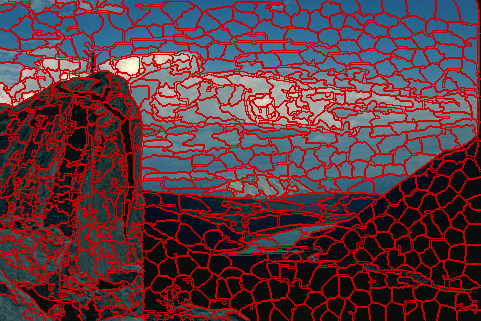
\includegraphics[scale=\scalefivebsd]{pictures/bsd-1-seeds-revised-spatial-mean-pixels}
	}
	\subfigure{
		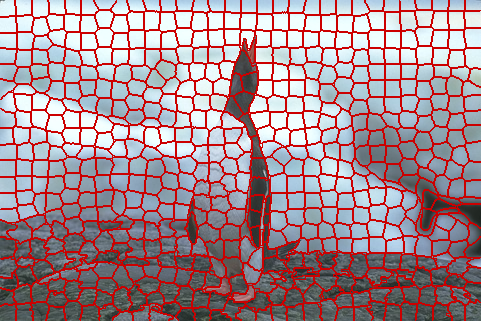
\includegraphics[scale=\scalefivebsd]{pictures/bsd-2-slic}
	}
	\subfigure{
		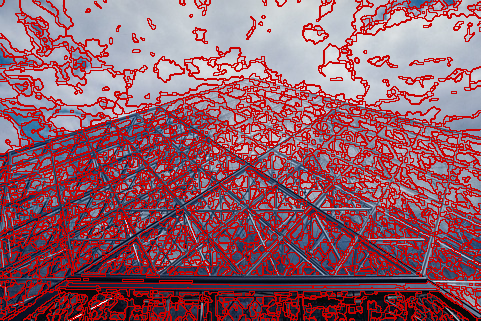
\includegraphics[scale=\scalefivebsd]{pictures/bsd-3-fh}
	}
	\subfigure{
		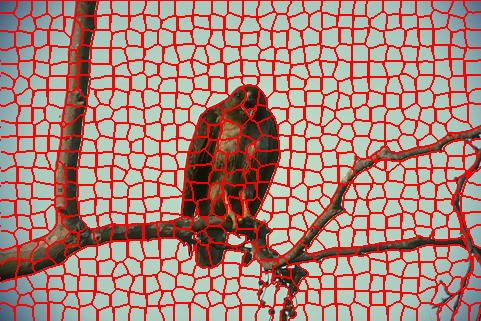
\includegraphics[scale=\scalefivebsd]{pictures/bsd-4-tp}
	}
	\subfigure{
		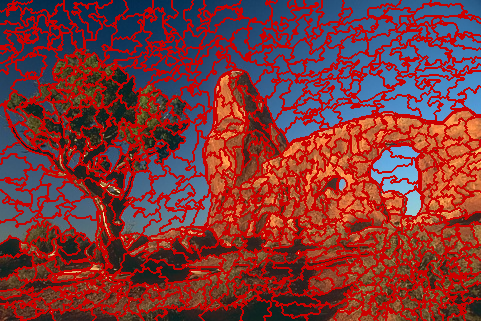
\includegraphics[scale=\scalefivebsd]{pictures/bsd-5-ers}
	}
	\subfigure{
		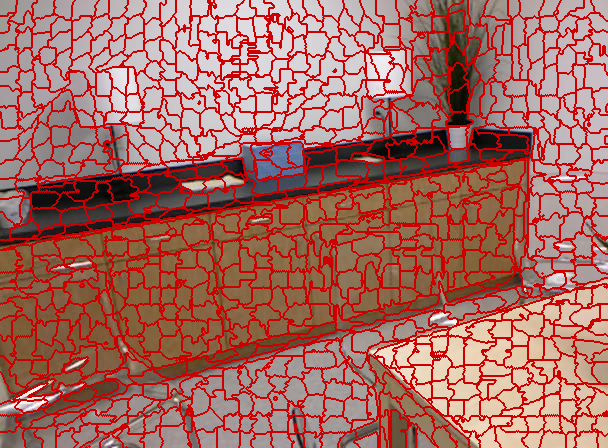
\includegraphics[scale=\scalefivenyu]{pictures/nyu-1-crs}
	}
	\subfigure{
		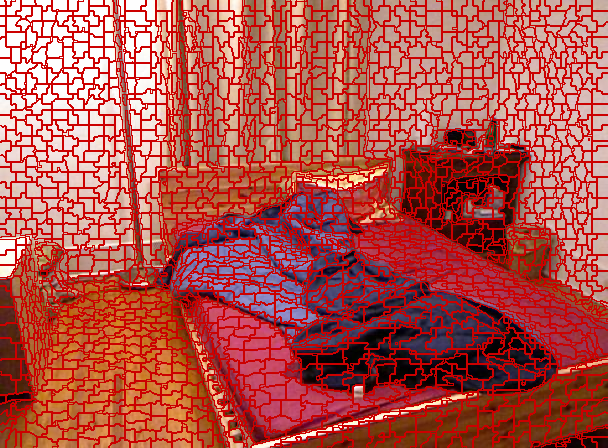
\includegraphics[scale=\scalefivenyu]{pictures/nyu-2-vccs}
	}
	\subfigure{
		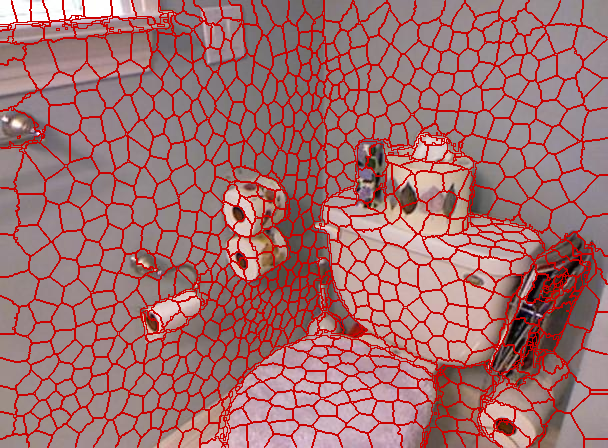
\includegraphics[scale=\scalefivenyu]{pictures/nyu-3-dasp}
	}
	\subfigure{
		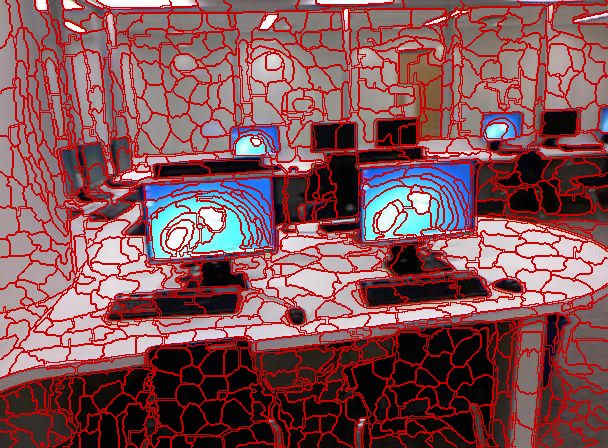
\includegraphics[scale=\scalefivenyu]{pictures/nyu-4-seeds3d}
	}
	\subfigure{
		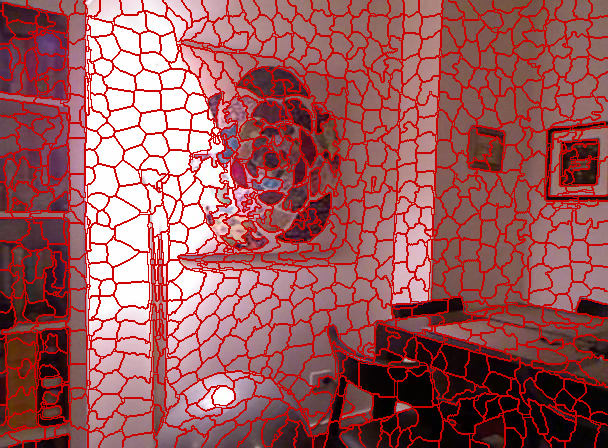
\includegraphics[scale=\scalefivenyu]{pictures/nyu-5-slic3d}
	}
	\caption[The running examples of this thesis taken from the Berkeley Segmentation Dataset \cite{ArbelaezMaireFowlkesMalik:2011} and the NYU Depth Dataset \cite{SilbermanHoiemKohliFergus:2012}.]{The running examples of this thesis will be used to introduce and evaluate several superpixel algorithms. Top: images taken from the Berkeley Segmentation Dataset \cite{ArbelaezMaireFowlkesMalik:2011} oversegmented into roughly $600$ superpixels. Bottom: images taken from the NYU Depth Dataset \cite{SilbermanHoiemKohliFergus:2012} oversegmented into roughly $840$ superpixels.}
	\label{fig:introduction-running-examples}
\end{figure}

% applications: \cite{ShuWangHuchuanLuFanYangMingHsuanYang:2011, FanYangHuchuanLuMingHsuanYang:2014, YuhangZhangHartleyMashfordBurn:2011, JainTuragaBriggmanHelmstadterDenkSeung:2011, GuptaArbelaezMalik:2013, RenMalik:2003, TigheLazebnik:2010, VanDenBerghRoigBoixManenVanGool:2013}
% algorithms: \cite{AchantaShajiSmithLucchiFuaSuesstrunk:2010, LiuTuzelRamalingamChellappa:2011, LevinshteinStereKutulakosFleetDickinsonSiddiqi:2009, MoorePrinceWarrellMohammedJones:2008, MoorePrinceWarrell:2010, VekslerBoykovMehrani:2010, ZengWangWangGanZha:2011, ZhangHartleyMashfordBurn:2011, VanDenBerghBoixRoigCapitaniVanGool:2012, WeikersdorferGossowBeetz:2012, PaponAbramovSchoelerWoergoetter:2013, ConradMertzMester:2013, DaiTangHuazhaFuXiaochunCao:2012, PerbetStengerMaki:2012, SivaWong:2014, RohkohlEngel:2007, DruckerMacCormick:2009}
Since their introduction, superpixels have actively been used for a wide range of applications: for example as pre-processing step for classical segmentation \cite{RenMalik:2003,RohkohlEngel:2007}, as mid-level cues used for tracking \cite{ShuWangHuchuanLuFanYangMingHsuanYang:2011}, as pre-processing step for graph-based stereo matching \cite{YuhangZhangHartleyMashfordBurn:2011}, or for semantic segmentation \cite{GuptaArbelaezMalik:2013}. In addition, numerous superpixel algorithms have been proposed. Although it may depend on the application which of these algorithms is preferable, most authors agree on the following basic requirements for superpixels \cite{LevinshteinStereKutulakosFleetDickinsonSiddiqi:2009,AchantaShajiSmithLucchiFuaSuesstrunk:2010,LiuTuzelRamalingamChellappa:2011}:
\begin{itemize}
	\item Superpixels should respect object boundaries;
	\item Superpixels should be generated as efficiently as possible;
	\item Superpixels should not lower the achievable performance\footnote{Here and in the following, performance refers to the quality of a superpixel segmentation rather than its runtime.} of subsequent processing steps.
\end{itemize}
Additional requirements may include compactness, especially in regions where no object boundaries are present \cite{LevinshteinStereKutulakosFleetDickinsonSiddiqi:2009,SchickFischerStiefelhagen:2012}, as well as connectivity \cite{LevinshteinStereKutulakosFleetDickinsonSiddiqi:2009}.

% video superpixels: \cite{AchantaShajiSmithLucchiFuaSuesstrunk:2012, ResoJachalskyRosenhahnOstermann:2013, ChangDonglaiWeiFisher:2013, HuazhuFuXiaochunCaoDaiTangYahongHanDongXu:2014, VanDenBerghRoigBoixManenVanGool:2013}
Until 2012, superpixel algorithms were designed to oversegment images with respect to the requirements stated above. However, with rising availability of low-cost RGB-D cameras, algorithms utilizing depth information become increasingly interesting for applications. Furthermore, extending the idea of superpixel segmentation to the temporal domain of videos is receiving increased attention. Approaches using depth information to oversegment videos \cite{WeikersdorferSchickCremers:2013} have recently been proposed. While some superpixel algorithms can naturally be extended to depth or video data, others may be constrained to color images or need to be adapted. One of the latter, although easily generalized to process video data \cite{VanDenBerghRoigBoixManenVanGool:2013}, is the approach proposed by Van den Bergh \etal \cite{VanDenBerghBoixRoigCapitaniVanGool:2012}, called \textbf{SEEDS}\footnote{\textbf{SEEDS} stands for ``Superpixels Extracted via Energy-Driven Sampling'' \cite{VanDenBerghBoixRoigCapitaniVanGool:2012}, see chapter \ref{chapter:superpixel-segmentation} for details.}. As \textbf{SEEDS} represents a superpixel algorithm showing both excellent runtime as well as state-of-the-art performance, the focus of this thesis lies in integrating depth information into \textbf{SEEDS}. Our goal is to preserve the low runtime while increasing performance by utilizing depth information.

% Another focus of this thesis is of comparative nature. Despite of the daunting number of superpixel algorithms available, only few research is devoted to comparing and analyzing the different approaches within a consistent framework: \cite{SchickFischerStiefelhagen:2012, NeubertProtzel:2012} and \cite{AchantaShajiSmithLucchiFuaSuesstrunk:2012}. While suitable datasets as for example the Berkeley Segmentation Dataset \cite{ArbelaezMaireFowlkesMalik:2011} or the NYU Depth Dataset \cite{SilbermanHoiemKohliFergus:2012} are available, used evaluation measures, as for example the Undersegmentation Error, are not defined consistently \cite{NeubertProtzel:2012, AchantaShajiSmithLucchiFuaSuesstrunk:2012} and implementations are mostly not made publicly available to reproduce the results presented in the corresponding publications. Another important aspect to consider, although this may seem trivial, is the availability of implementations for different platforms. Most algorithms are implemented using MatLab or C/C++ using a wide range of different libraries. Often the actual implementations differ from the proposed algorithm, as for example \textbf{SEEDS}, or details concerning the implementation are not discussed in detail. Therefore, it is difficult to determine both the state-of-the-art as well as algorithms suited for specific applications.

Another focus of this thesis lies in a comparative assessment of all superpixel algorithms providing source code. We find this necessary as only few research is devoted to comparing and evaluating the rising number of approaches within a consistent framework. To the best of our knowledge these are \cite{SchickFischerStiefelhagen:2012, NeubertProtzel:2012} and \cite{AchantaShajiSmithLucchiFuaSuesstrunk:2012}. We base our experiments on both the Berkeley Segmentation Dataset \cite{ArbelaezMaireFowlkesMalik:2011} as well as the NYU Depth Dataset \cite{SilbermanHoiemKohliFergus:2012}. While the Berkeley Segmentation Dataset is commonly used to assess superpixel algorithms, performance on the NYU Depth Dataset may be of particular interest for specific applications. In particular, the scenes captured by the NYU Depth Dataset provide a fresh contrast to the natural images from the Berkeley Segmentation Dataset. Additionally, it provides depth images allowing us to evaluate additional algorithms requiring depth information. Furthermore, widely used evaluation measures are not defined consistently throughout the literature, as for example the Undersegmentation Error \cite{NeubertProtzel:2012, AchantaShajiSmithLucchiFuaSuesstrunk:2012}. Another commonly used measure is Boundary Recall \cite{MartinFowlkesMalik:2004}. However, evaluation based on these two measures only may give a highly biased impression such that an assessment using additional measures is necessary. Finally, details concerning the available implementations, as well as the parameter selection is often omitted within the corresponding publications. Overall, it is difficult to determine both the state-of-the-art as well as approaches suited for specific applications. In our opinion, this is highly unsatisfactory.

\section{Contributions}

The main contributions of this thesis are:~
\begin{itemize}
	\item An implementation of \textbf{SEEDS} including a variant providing a compactness parameter \cite{VanDenBerghBoixRoigVanGool:2013} and several extensions utilizing depth information.
	\item A thorough evaluation of several superpixel algorithms on the Berkeley Segmentation Dataset and the NYU Depth Dataset using an extended version of the Berkeley Segmentation Benchmark providing additional measures to evaluate superpixel algorithms.
\end{itemize}
The extended Berkeley Segmentation Benchmark is made publicly available together with our implementation of \textbf{SEEDS}.

\section{Outline}

The thesis is organized as follows: After this short introduction, chapter \ref{chapter:related-work} reviews the literature on superpixel algorithms. Chapter \ref{chapter:superpixel-segmentation} gives a thorough introduction to \textbf{SEEDS} as well as another superpixel algorithm used as baseline, called \textbf{SLIC}\footnote{\textbf{SLIC} stands for ``Simple Linear Iterative Clustering'', see chapter \ref{chapter:related-work} for details.}~\cite{AchantaShajiSmithLucchiFuaSuesstrunk:2010}. Then, chapter \ref{chapter:superpixel-segmentation-depth} discusses several approaches to superpixel segmentation utilizing depth information. This includes a detailed discussion of integrating depth information into \textbf{SLIC}. Chapter \ref{chapter:seeds-depth} represents the main part of this thesis and discusses several extensions of \textbf{SEEDS} to depth. We present several variants of \textbf{SEEDS} using depth information and focus on two of them for evaluation. The datasets and measures used for evaluation are discussed in chapter \ref{chapter:datasets}. Chapter \ref{chapter:evaluation} presents experimental results of several superpixel algorithms. Parameters are optimized individually on training/validation sets before the different algorithms are compared on the corresponding test sets with regard to their qualitative and quantitative performance as well as runtime. Chapter \ref{chapter:conclusion} gives a short conclusion, a brief outlook and presents ideas for future work in this area.

% The appendix includes documentation of the Berkeley Segmentation Benchmark, as we found that the benchmark lacks detailed documentation, the Extended Berkeley Segmentation Benchmark as well as further tables and figures concerning the qualitative and quantitative comparison given in chapter \ref{chapter:evaluation}.

%\section{Nomenclature}
%
%We use the term \textit{superpixel algorithm}\index{superpixel algorithm} to denote an algorithm generating an oversegmentation of a RGB or RGB-D image. The terms \textit{oversegmentation} and \textit{superpixel segmentation} are used interchangeably. The terms \textit{supervoxel} and \textit{temporal supervoxel}, as introduced in chapter \ref{chapter:related-work}, are used to denote a segmentation of a point cloud and a video sequence, respectively. The term \textit{superpixel} always denotes a single, connected segment within a superpixel segmentation. The same goes for supervoxel and temporal supervoxel in their respective domains.
\chapter{Related Work}
\label{chapter:related-work}

Research related to superpixel algorithms has seen a substantial growth during the last few years (see figure \ref{fig:related-work-superpixel-timeline}). Consequently, the literature on this topic is quite extensive. In this chapter, we try to cover the literature \textbf{to the best of our knowledge} and give a brief introduction to all superpixel algorithms evaluated in chapter \ref{chapter:evaluation}. We divide all algorithms presented in this chapter into those applicable to color images, those utilizing depth information and those used to oversegment point clouds. Furthermore, we review the literature devoted to comparing these approaches as well as suitable datasets and benchmarks.

\section{Superpixel Segmentation}
\label{section:related-work-superpixel-segmentation}

Throughout the literature, superpixel algorithms are often categorized as either graph based methods or gradient ascent methods \cite{AchantaShajiSmithLucchiFuaSuesstrunk:2012}. Both expect a color image $I : \ubar{W} \times \ubar{H} \rightarrow \mathbb{R}^3$, $\ubar{W} = \{1, \ldots, W\}$, with width $W$, height $H$ and $N = WH$ pixels to be given and aim to generate a superpixel segmentation
\begin{align}
	S = \{S_1,\ldots,S_K\}\quad \text{ with }\quad S_k \subseteq \ubar{W} \times \ubar{H}.
\end{align}
For this superpixel segmentation to be valid, we demand the superpixels $S_i$ to represent connected components \cite{LevinshteinStereKutulakosFleetDickinsonSiddiqi:2009}. Additionally, we enforce the superpixels to be disjoint and resemble the whole image:
\begin{align}
	S_i \cap S_j = \emptyset\quad \text{ and }\quad \bigcup_{S_i \in S} S_i = \ubar{W} \times \ubar{H}.
\end{align}
Then, we can define the function $s: \ubar{W} \times \ubar{H} \rightarrow \ubar{K}$ assigning a unique superpixel to each pixel $x_n \in \ubar{W} \times \ubar{H}$.

Graph based approaches construct an undirected, weighted graph $G = (V,E)$ with $V = \ubar{N}$ where each vertex $n$ corresponding to pixel $x_n$ is connected to the pixel's four direct neighbors\footnote{This resembles a $4$-connected graph. However, some approaches and applications use a $8$-connected graph, instead, where each pixel $x_n$ is connected to its diagonal neighbors as well.}. The weights $w_{n,m}$ are interpreted as elements of a weight matrix
\begin{align}
	\boldsymbol{w} = \left (w_{n,m}\right)_{n,m = 1}^N
\end{align}
where $w_{n,m}$ measures the similarity of neighboring pixels $x_n$ and $x_m$ and we set $w_{n,m} = 0$ for $(n,m) \notin E$. Typically, an energy based on the graph $G$ is proposed and optimized using graph cuts or similar techniques.

Gradient ascent methods are commonly built around an energy as well, however, these methods are not based on a graph structure. Instead, they use a variety of different approaches to optimize the proposed energy in order to generate a superpixel segmentation. For example, clustering based approaches define the superpixel center of superpixel $S_i$ to be given by
\begin{align}
	\mu(S_i) = \frac{1}{|S_i|} \sum_{x_n \in S_i} x_n\quad \text{ and }\quad I(S_i) = \frac{1}{|S_i|} \sum_{x_n \in S_i} I(x_n).
\end{align}
Then, pixels are assigned to superpixels based on their similarity to the superpixel centers.

Although the categorization into graph based and gradient ascent methods appears to be very coarse, a finer categorization lies not in the focus of this thesis. In the following we briefly introduce all superpixel algorithms evaluated in chapter \ref{chapter:evaluation}. The algorithms are sorted according to the year of their publication. Figure~\ref{fig:related-work-superpixel-timeline} shows a timeline of all superpixel algorithms.
\begin{figure}[t!]
	\centering
	\begin{tikzpicture}
		% line
		\draw (0.25,0) -- (3,0);
		\draw (3,-0.25) -- (3.25,0.25);
		\draw (3.25,-0.25) -- (3.5,0.25);
		\draw[-latex new,arrow head=0.15cm] (3.5,0) -- (14.5,0);
		
		% years
		\draw (0.75,0.15) -- (0.75,-0.15);
		\node at (0.75,-0.5){2003};
		\draw (2,0.15) -- (2,-0.15);
		\node at (2,-0.5){2004};
		
		\draw (4.5,0.15) -- (4.5,-0.15);
		\node at (4.5,-0.5){2007};
		\draw (5.75,0.15) -- (5.75,-0.15);
		\node at (5.75,-0.5){2008};
		\draw (7,0.15) -- (7,-0.15);
		\node at (7,-0.5){2009};
		\draw (8.25,0.15) -- (8.25,-0.15);
		\node at (8.25,-0.5){2010};
		\draw (9.5,0.15) -- (9.5,-0.15);
		\node at (9.5,-0.5){2011};
		\draw (10.75,0.15) -- (10.75,-0.15);
		\node at (10.75,-0.5){2012};
		\draw (12,0.15) -- (12,-0.15);
		\node at (12,-0.5){2013};
		\draw (13.25,0.15) -- (13.25,-0.15);
		\node at (13.25,-0.5){2014};
		
		% algorithms
		% Ncut
		\draw (0.75,0.15) -- (0.75,0.5) -- (0.9,0.75);
		\node at (1.25,0.75){\textbf{NC}};
		
		% F&H
		\draw (2,0.15) -- (2,0.5) -- (2.15,0.75);
		\node at (2.5,0.75){\textbf{FH}};
		
		% SPPS
		\draw (4.5,0.15) -- (4.5,0.5) -- (4.65,0.75);
		\node at (5.2,0.75){\textbf{SPPS}};
		
		% QS
		\draw (5.75,0.15) -- (5.75,0.5) -- (5.9,0.75);
		\node at (6.25,0.75){\textbf{QS}};
		
		% SL
		\draw (5.75,-0.75) -- (5.75,-1) -- (5.9,-1.25);
		\node at (6.25,-1.25){\textbf{SL}};
		
		% TP
		\draw (7,0.15) -- (7,0.5) -- (7.15,0.75);
		\node at (7.5,0.75){\textbf{TP}};
		
		% SSP
		\draw (7,-0.75) -- (7,-1) -- (7.15,-1.25);
		\node at (7.65,-1.25){\textbf{SSP}};
		
		% SLIC
		\draw (8.25,0.15) -- (8.25,0.5) -- (8.4,0.75);
		\node at (9,0.75){\textbf{SLIC}};
		
		% CIS
		\draw (8.25,-0.75) -- (8.25,-1) -- (8.4,-1.25);
		\node at (8.85,-1.25){\textbf{CIS}};
		
		% ERS
		\draw (9.5,0.15) -- (9.5,0.5) -- (9.65,0.75);
		\node at (10.1,0.75){\textbf{ERS}};
		
		% PB
		\draw (9.5,-0.75) -- (9.5,-1) -- (9.65,-1.25);
		\node at (10,-1.25){\textbf{PB}};
		
		% SSS
		\draw (9.5,-1.25) -- (9.5,-1.5) -- (9.65,-1.75);
		\node at (10.1,-1.75){\textbf{SSS}};
		
		% CRS
		\draw (9.5,-1.75) -- (9.5,-2) -- (9.65,-2.25);
		\node at (10.1,-2.25){\textbf{CRS}};
		
		% HS
		\draw (9.5,-2.25) -- (9.5,-2.5) -- (9.65,-2.75);
		\node at (10,-2.75){\textbf{HS}};
		
		\draw (10.75,2.25) -- (10.75,2.5) -- (10.9,2.75);
		\node at (11.65,2.75){\cite{SchickFischerStiefelhagen:2012}};
		
		\draw (10.75,1.75) -- (10.75,2) -- (10.9,2.25);
		\node at (11.8,2.25){\cite{AchantaShajiSmithLucchiFuaSuesstrunk:2012}};
		
		\draw (10.75,1.25) -- (10.75,1.5) -- (10.9,1.75);
		\node at (11.55,1.75){\cite{NeubertProtzel:2012}};
		
		% SEEDS
		\draw (10.75,0.75) -- (10.75,1) -- (10.9,1.25);
		\node at (11.65,1.25){\textbf{SEEDS}};
		
		% DASP
		\draw (10.75,0.15) -- (10.75,0.5) -- (10.9,0.75);
		\node at (11.5,0.75){\textbf{DASP}};
		
		% TPS 
		\draw (10.75,-0.75) -- (10.75,-1) -- (10.9,-1.25);
		\node at (11.35,-1.25){\textbf{TPS}};
		
		% VCCS
		\draw (12,-0.75) -- (12,-1) -- (12.15,-1.25);
		\node at (12.75,-1.25){\textbf{VCCS}};
		
		% TPS
		\draw (12,-1.25) -- (12,-1.5) -- (12.15,-1.75);
		\node at (12.65,-1.75){\textbf{TPS}};
		
		% TS
		%\draw (12,-1.75) -- (12,-2) -- (12.15,-2.25);
		%\node at (12.5,-2.25){\textbf{TS}};
		
		% DASV
		%\draw (12,-2.75) -- (12,-3) -- (12.15,-3.25);
		%\node at (12.75,-3.25){\textbf{DASV}};
		
		% RPS
		%\draw (13.25,0.15) -- (13.25,0.5) -- (13.4,0.75);
		%\node at (13.85,0.75){\textbf{RPS}};
		
		% GSS
		%\draw (13.25,0.75) -- (13.25,1) -- (13.4,1.25);
		%\node at (13.85,1.25){\textbf{GSS}};
	\end{tikzpicture}
	\caption[Timeline of superpixel, supervoxel and temporal supervoxel algorithms. Publications on comparing these approaches are shown as well.]{Timeline of proposed superpixel, supervoxel and temporal supervoxel algorithms. See sections \ref{section:related-work-superpixel-segmentation}, \ref{section:related-work-superpixel-segmentation-using-depth} and \ref{section:section:related-work-supervoxel-segmentation} for the used abbreviations. In this context, three publications devoted to the comparison of superpixel algorithms are shown, see section \ref{section:related-work-comparison}.
	%Legend: \textbf{NC}: Superpixels from Normalized Cuts \cite{RenMalik:2003}; \textbf{FH} Graph based superpixels by Felzenswalb \& Huttenlocher \cite{FelzenswalbHuttenlocher:2004}; \textbf{SPPS}: Superpixels using Pairwise Pixel Similarities \cite{RohkohlEngel:2007}; \textbf{QS}: QuickShift \cite{VedaldiSoatto:2008}; \textbf{SL}: Superpixel Lattices \cite{MoorePrinceWarrellMohammedJones:2008}; \textbf{TP}: Turbopixels \cite{LevinshteinStereKutulakosFleetDickinsonSiddiqi:2009}; \textbf{SSP} Superpixels from Strong Paths \cite{DruckerMacCormick:2009};\textbf{SLIC}: Simple Linear Iterative Clustering \cite{AchantaShajiSmithLucchiFuaSuesstrunk:2010}; \textbf{CIS}: Constant Intensity Superpixels \cite{VekslerBoykovMehrani:2010}; \textbf{ERS}: Entropy Rate Superpixels \cite{LiuTuzelRamalingamChellappa:2011}; \textbf{PB}: Superpixels via Pseudo-Boolean Optimization \cite{ZhangHartleyMashfordBurn:2011}; \textbf{SSS}: Structure Sensitive Superpixels \cite{ZengWangWangGanZha:2011}; \textbf{DASP}: Depth-Adaptive Superpixels \cite{WeikersdorferGossowBeetz:2012}; \textbf{HS}: Homogeneous Superpixels \cite{PerbetStengerMaki:2012}; \textbf{TPS}: Topology Preserved Superpixels; \textbf{SEEDS}: Superpixels Extracted via Energy-Driven Sampling \cite{VanDenBerghBoixRoigCapitaniVanGool:2012}; \textbf{VCCS}: Voxel-Cloud Connectivity Segmentation \cite{PaponAbramovSchoelerWoergoetter:2013}; \textbf{CRS}: Contour-Relaxed Superpixels \cite{ConradMertzMester:2013}; \textbf{TCS}: Temporally Consistent Superpixels \cite{ResoJachalskyRosenhahnOstermann:2013}; \textbf{TS}: Temporal Superpixels \cite{ChangDonglaiWeiFisher:2013}; \textbf{DASV}: Depth-Adaptive Supervoxels \cite{WeikersdorferSchickCremers:2013}; \textbf{RPS}: Regularity Preserving Superpixels \cite{HuazhuFuXiaochunCaoDaiTangYahongHanDongXu:2014}; \textbf{GSS}: Grid Seams Superpixels \cite{SivaWong:2014}.
	}
	\label{fig:related-work-superpixel-timeline}
\end{figure}

%\textbf{NC} -- Superpixels from Normalized Cuts \cite{RenMalik:2003}. The normalized cuts algorithm was originally proposed in 2000 by Shi \etal \cite{ShiMalik:2000} for the task of classical segmentation. In 2003, Ren \etal \cite{RenMalik:2003} used normalized cuts as integral component for the very first superpixel algorithm. The normalized cuts algorithm is a graph based algorithm using graph cuts to optimize a global energy function.
%
%\textbf{FH} -- Felzenswalb \& Huttenlocher \cite{FelzenswalbHuttenlocher:2004}. Proposed in 2004, this is another graph based approach which was originally not intended to generate superpixel segmentations. The algorithm is based on a predicate describing whether there is evidence for a boundary between to segments. Using an initial segmentation where each pixel is its own segment, the algorithm merges segments based on this predicate.
%
%\textbf{QS} -- QuickShift \cite{VedaldiSoatto:2008}. Proposed four years later in 2008, \textbf{QS} can be categorized as gradient ascent method and is a mode-seeking algorithm. It was originally not intended as superpixel algorithm. After estimating a density $p(x_n)$ for each pixel $x_n$, the algorithm follows the gradient of the density to assign each pixel to a mode. The modes represent the final segments.
%
%\textbf{TP} -- Turbopixels \cite{LevinshteinStereKutulakosFleetDickinsonSiddiqi:2009}. In 2009, this was one of the first algorithms explicitly designed to obtain superpixel segmentations (\ie after \cite{RohkohlEngel:2007}). Turbopixels is an algorithm inspired by active contours. After selecting initial superpixel centers, each superpixel is grown by the means of an evolving contour. 
%
%\textbf{SLIC} -- Simple Linear Iterative Clustering \cite{AchantaShajiSmithLucchiFuaSuesstrunk:2010}. Proposed in 2010, this algorithm is often used as baseline \cite{HuazhuFuXiaochunCaoDaiTangYahongHanDongXu:2014, PaponAbramovSchoelerWoergoetter:2013, VanDenBerghBoixRoigCapitaniVanGool:2012, ConradMertzMester:2013} and is particular interesting because of its simplicity. \textbf{SLIC} implements a local $K$-means clustering to generate a superpixel segmentation with $K$ superpixels. Therefore, \textbf{SLIC} can be categorized as gradient ascent method. The algorithm is discussed in detail in chapter~\ref{chapter:superpixel-segmentation}.
%
%\textbf{CS} and \textbf{CIS} -- Compact Superpixels and Constant Intensity Superpixels \cite{VekslerBoykovMehrani:2010}. Both proposed in \cite{VekslerBoykovMehrani:2010}, these are two additional graph based methods. In addition, both approaches are defined on grayscale images. Initially, the image is covered by overlapping squares such that each pixel is covered by several squares. Each square represents a superpixel and each pixel can get assigned to one of the overlapping squares. The assignment for each pixel is computed using $\alpha$-expansion \cite{BoykovVekslerZabih:2001}.
%
%\textbf{ERS} -- Entropy Rate Superpixels \cite{LiuTuzelRamalingamChellappa:2011}. This algorithm is another graph based method and was proposed in 2011 \cite{LiuTuzelRamalingamChellappa:2011}. An objective function based on the entropy rate of a random walk on the graph $G$ is proposed. The energy function consists of a color term, encouraging superpixels with homogeneous color, and a boundary term, favoring superpixels of similar size.
%
%\textbf{PB} -- Superpixels via Pseudo Boolean Optimization \cite{ZhangHartleyMashfordBurn:2011}. Proposed in 2011, this algorithm is comparable to \textbf{CS} and \textbf{CIS}. First, the image is overlayed by overlapping vertical and horizontal strips such that each pixel is covered by exactly two vertical strips and two horizontal strips. This way, considering only the horizontal strips, each pixel is either labeled $0$ or $1$. The assignment is computed using max-flow (see \cite{ZhangHartleyMashfordBurn:2011} for details). Together, the labels corresponding to the horizontal strips and the labels of the vertical strips form a superpixel segmentation.
%
%\textbf{SEEDS} -- Superpixels Extracted via Energy-Driven Sampling \cite{VanDenBerghBoixRoigCapitaniVanGool:2012}. Proposed in 2013, this algorithm can be categorized as gradient ascent method and is the main focus of this thesis. The authors propose a highly competitive algorithm which is limited to color images. The algorithm is discussed in detail in chapter \ref{chapter:superpixel-segmentation} and approaches to generalize the algorithm to RGB-D images are reviewed in chapter \ref{chapter:seeds-depth}.
%
%\textbf{TPS} -- Topology Preserved Superpixels \cite{DaiTangHuazhaFuXiaochunCao:2012}. \textbf{TPS} aims to generate a superpixel segmentation representing a regular grid topology, that is the superpixels can be arranged in an array where each superpixel has a consistent, ordered position \cite{DaiTangHuazhaFuXiaochunCao:2012}. Therefore, after choosing a set of pixels as initial grid positions, these positions are shifted to the maximum edge positions based on a provided edge map. Then, the positions define an undirected graph based on the relative positions. Neighboring grid positions are connected using shortest paths in a weighted graph, where the weight between two pixels is inverse proportional to the edge probability of those pixels.
%
%\textbf{CRS} -- Contour Relaxed Superpixels \cite{ConradMertzMester:2013}. This approach, proposed in 2013 \cite{ConradMertzMester:2013}, represents a statistical approach to the task of superpixel segmentation where the image $I$ is assumed to be a result of multiple stochastic processes. Actually, the value of pixel $x_n$ in channel $c$ is thought to be an outcome of a stochastic process specific to the corresponding superpixel. An energy is derived which is optimized using a hill-climbing algorithm.

\textbf{NC} -- Superpixels from Normalized Cuts \cite{RenMalik:2003}. The Normalized Cuts algorithm was originally proposed in 2000 by Shi and Malik \cite{ShiMalik:2000} for the task of classical image segmentation. In 2003, Ren and Malik \cite{RenMalik:2003} used Normalized Cuts as integral component for the very first superpixel algorithm. As graph based approach, the algorithm successively adds graph cuts in order to oversegment the image where each graph cut minimizes a global criterion called Normalized Cut:
\begin{align}
	NCut(A,B) = \frac{cut(A,B)}{assoc(A,V)} + \frac{cut(A,B)}{assoc(B,V)}
\end{align}
where $A,B \subseteq V$ are the two segments resulting from the cut and
\begin{align}
	cut(A,B) &= \sum_{n \in A} \sum_{m \in B} w_{n,m},\\
	assoc(A, V) &= \sum_{n \in A} \sum_{m \in V} w_{n,m}.
\end{align}
As shown in \cite{ShiMalik:2000}, this criterion can be minimized by discretizing the second smallest eigenvalue corresponding to the generalized eigenvalue problem
\begin{align}
	(\boldsymbol{d} - \boldsymbol{w})y = \lambda \boldsymbol{d} y
\end{align}
where $\boldsymbol{d}$ is a diagonal matrix with $d_{n,n} = \sum_{m \in V} w_{n,m}$. To obtain superpixels, this criterion can be applied recursively or additional eigenvectors (third smallest eigenvector \etc) can be used \cite{RenMalik:2003}.

\begin{algorithm}[t]
	\begin{algo}{}{\label{algo:related-work-fh}\qinput{undirected, weighted graph $G = (V,E)$}\qoutput{superpixel segmentation $S$}}
		sort $E$ by increasing edge weight\\
		let $S$ be the superpixel segmentation where each pixel is its own superpixel\\
		\qfor $k = 1$ \qto $|E|$\\
			let $(n,m)$ be the $k^\text{th}$ edge\\
			\qif $s(x_n) \neq s(x_m)$\\
			\qthen \qif $w_{n,m}$ is sufficiently small compared to $MInt(S_{s(x_n)}, S_{s(x_m)})$\\
				\qthen merge superpixels $S_{s(x_n)}$ and $S_{s(x_m)}$\qfi\qfi\qrof\\
		\qreturn $S$
	\end{algo}
	\caption{The superpixel algorithm \textbf{FH} proposed in \cite{FelzenswalbHuttenlocher:2004}.}
	\label{fig:related-work-fh-algorithm}
\end{algorithm}
\textbf{FH} -- Felzenswalb \& Huttenlocher \cite{FelzenswalbHuttenlocher:2004}. Proposed in 2004 by Felzenswalb and Huttenlocher, this is another graph based approach summarized in algorithm \ref{algo:related-work-fh}. For $A \subseteq V$, we define $MST(A)$ to be the set of edges corresponding to the minimum spanning tree of $A$ within the graph $G = (V,E)$ and define
\begin{align}
	\label{eq:related-work-fh}
	Int(A) &= \max_{(n,m) \in MST(A)} \{w_{n,m}\},\\
	MInt(A, B) &= \min \{Int(A) + \frac{\tau}{|A|}, Int(B) + \frac{\tau}{|B|}\}
\end{align}
where $\tau$ is a threshold parameter and $MInt(A,B)$ is called the minimum internal difference of components $A$ and $B$. Starting from an initial superpixel segmentation where each pixel forms its own superpixel, the algorithm processes all edges sorted by increasing edge weight. Whenever an edge connects two different superpixels, these are merged if the edge weight is small compared to the minimum internal difference.% In their paper, Felzenswalb and Huttenlocher proof that this approach produces a segmentation which is neither too coarse nor too fine.

\textbf{QS} -- QuickShift \cite{VedaldiSoatto:2008}. Proposed four years later in 2008, \textbf{QS} can be categorized as gradient ascent method and is a mode-seeking algorithm. In general, a mode-seeking algorithm starts from a Parzen density estimate $p(x_n)$ for all pixels and each pixel is assigned to a mode by following the density $p(x_n)$ upwards, that is in the direction of the gradient \cite{VedaldiSoatto:2008}. In particular, \textbf{QS} pre-computes $p(x_n)$ for all pixels using a Gaussian kernel. In practice, the distance $d(x_n,x_m)$ used within the Gaussian kernel consists of a color term and a spatial term:
\begin{align}
	\label{eq:related-work-quickshift-distance}
	d(x_n,x_m) = \alpha\|I(x_n) - I(x_m)\|_2 + \|x_n - x_m\|_2
\end{align}
where $\alpha$ weights the influence of the color term. Subsequently, each pixel $x_n$ gets assigned to the pixel $x_m \in N_R(x_n) = \{x_m : \|x_n - x_m\|_\infty \leq \floor*{R/2}\}$ such that $p(x_m) > p(x_n)$ or is left unassigned. These assignments correspond to the found modes, representing the final superpixels. This procedure is summarized in algorithm \ref{algo:related-work-qs}.
\begin{algorithm}[t]
	\begin{algo}{QS}{\label{algo:related-work-qs}\qinput{color image $I$}\qoutput{superpixel segmentation $S$}}
		\qfor $n = 1$ \qto $N$\\
			initialize $t(x_n) = \boldsymbol 0$\qrof\\
		\qfor $n = 1$ \qto $N$\\
			\qcom{$N_R(x_n)$ is the set of all pixels in the local neighborhood of size $R \times R$ around pixel $x_n$:}\\
			calculate $p(x_n) = \sum_{x_m \in N_R(x_n)} \exp\left(\frac{-d(x_n,x_m)^2}{(2/3) R}\right)$ \qrof\\
		\qfor $n = 1$ \qto $N$\\
			set $t(x_n) = \arg\max_{x_m \in N_R(x_n): p(x_m) > p(x_n)} \{p(x_m)\}$\qrof\\
		\qcom{$t$ maps each pixel to its neighbor $x_m$ with highest $p(x_m)$ if $p(x_m) > p(x_n)$;}\\
		\qcom{$t$ can be interpreted as forest, where all pixels $x_n$ with $t(x_n) = \boldsymbol 0$ are roots.}\\
		derive superpixel segmentation $S$ from $t$\\
		\qreturn $S$
	\end{algo}
	\caption{The superpixel algorithm \textbf{QS} proposed in \cite{VedaldiSoatto:2008}.}
	\label{fig:related-work-qs-algorithm}
\end{algorithm}

\textbf{TP} -- Turbopixels \cite{LevinshteinStereKutulakosFleetDickinsonSiddiqi:2009}. Proposed in 2009, Turbopixels is an algorithm inspired by active contours. After placing initial superpixel centers on a regular grid with step size $R$, each superpixel is grown based on an evolving contour. The contour is implemented as level set\footnote{That is, the superpixel boundaries are interpreted as the zero-level set of the function $\Psi$ (all points where $\Psi$ equals zero). See \cite{OsherFedkiw:2003} for details on level set methods.} of a smooth function $\Psi : \mathbb{R}^2 \times [0,\tau) \rightarrow \mathbb{R}^2$. Evolution is formally defined by the equation
\begin{align}
	\Psi_t = -  v \|\nabla\Psi\|_2
\end{align}
where $\nabla\Psi$ denotes the gradient of $\Psi$, $\Psi_t$ is the time derivative of $\Psi$ and the speed $v$ describes the future evolution of the contour. In practice, $\Psi$ will be the signed euclidean distance of each pixel to the contour \cite{LevinshteinStereKutulakosFleetDickinsonSiddiqi:2009} and the evolution is carried out using a first order discretization such that the contour in iteration $(T+1)$ is given by
\begin{align}
	\label{eq:related-work-tp-evolution}
	\Psi^{(T+1)} = \Psi^{(T)} - v_I v_B \|\nabla\Psi^{(T)}\| \Delta t
\end{align}
where $v_I$ depends on the image content, while $v_B$ ensures that superpixels do not overlap, see \cite{LevinshteinStereKutulakosFleetDickinsonSiddiqi:2009} for details. In each iteration $(T + 1)$, pixels $x_n$ for which $\Psi^{(T)} (x_n) > 0$ are considered unassigned. Iteratively, the superpixels are grown by computing the speeds $v_I$ and $v_B$ and evolving the contour according to equation \eqref{eq:related-work-tp-evolution} until all pixels are assigned. A summary is given in algorithm \ref{algo:related-work-turbopixels}.
\begin{algorithm}[t]
	\begin{algo}{TP}{\label{algo:related-work-turbopixels}\qinput{color image $I$, number of superpixels $K$}\qoutput{superpixel segmentation $S$}}
		% \qcom{seeds may be perturbed if necessary}\\
		\qcom{$R$ can be derived from the image size $W \times H$ and the number of superpixels $K$:}\\
		place superpixel centers on a regular grid with step size $R$\\
		\qcom{All pixels $x_n$ where $\Psi(x_n) > 0$ are unassigned.}\\
		initialize $\Psi^{(0)}$\\
		\qrepeat\\
			compute $v_I$ and $v_B$\\
			evolve the contour by computing $\Psi^{(T+1)}$\\
			update assigned pixels\\
			$T$ \qlet $T + 1$
		\quntil all pixels are assigned\\
		\qcom{A superpixel segmentation can be derived from the contour given by $\Psi$:}\\
		derive $S$ from $\Psi$\\
		\qreturn $S$
	\end{algo}
	\caption{The superpixel algorithm \textbf{TP} proposed in \cite{LevinshteinStereKutulakosFleetDickinsonSiddiqi:2009}.}
	\label{fig:related-work-tp-algorithm}
\end{algorithm}

\textbf{SLIC} -- Simple Linear Iterative Clustering \cite{AchantaShajiSmithLucchiFuaSuesstrunk:2010}. Proposed in 2010, this algorithm is often used as baseline, for example in \cite{HuazhuFuXiaochunCaoDaiTangYahongHanDongXu:2014, PaponAbramovSchoelerWoergoetter:2013, VanDenBerghBoixRoigCapitaniVanGool:2012} and \cite{ConradMertzMester:2013}, and is particular interesting because of its simplicity. \textbf{SLIC} implements a local $K$-means clustering to generate a superpixel segmentation with $K$ superpixels. Therefore, \textbf{SLIC} can be categorized as gradient ascent method. The algorithm is discussed in detail in chapter \ref{chapter:superpixel-segmentation}.

\textbf{CIS} -- Constant Intensity Superpixels \cite{VekslerBoykovMehrani:2010}. Proposed by Veksler \etal in 2010, this is a graph based method defined on grayscale images only. However, the below description is easily extended to color images. Initially, the image is covered by overlapping squares such that each pixel is covered by several squares. Each square represents a superpixel and each pixel can get assigned to one of these squares. An energy of the form
\begin{align}
	\label{eq:related-work-cis-energy}
	E(S) = \sum_{n \in V} \sum_{m \in V} w_{n,m} \psi_{n,m}(s(x_n), s(x_m)) + \sum_{n \in V} \theta_n(s(x_n))
\end{align}
is minimized using $\alpha$-expansion \cite{BoykovVekslerZabih:2001}. In particular, $\theta_n$ defines a data term which is simplified\footnote{Actually, instead of using $I(S_i)$ within the data term, the color of the center pixel of the initial square $S_i$ is used and fixed. However, this requires discussing an additional term ensuring that this center pixel is assigned to superpixel $S_i$ as well, see \cite{VekslerBoykovMehrani:2010}.} given by
%\begin{align}
%	\theta_n(i) = \begin{cases}
%		1 & \text{if } x_n \text{ is assigned to superpixel } S_i\\
%		0 & \text{else}
%	\end{cases}
%\end{align}
%in the case of Compact Superpixels and
\begin{align}
	\label{eq:related-work-cis-data-term}
	\theta_n(i) = \begin{cases}
		|I(x_n) - I(S_i)| & \text{if } x_n \text{ is assigned to superpixel } S_i\\
		0 & \text{else}
	\end{cases}.
\end{align}
\begin{algorithm}[t]
	\begin{algo}{ERS}{\label{algo:related-work-ers}\qinput{undirected, weighted graph $G = (V, E)$}\qoutput{superpixel segmentation $S$}}
		initialize $M = \emptyset$\\
		\qforeach edge $(n,m) \in E$\\
			\qcom{Let $\hat{G}$ denote the graph $\hat{G} = (V, M \cup \{(n, m)\})$:}\\
			choose edge $(n,m) \in E$ yielding the largest gain in the energy $E(\hat{G})$\\
			\qif $\hat{G}$ has no cycles and $\hat{G}$ contains less or equal than $K$ connected components\\
				\qthen $M$ \qlet $M \cup \{(n,m)\}$\qfi\qrof\\
		\qcom{The superpixel segmentation is given by the connected components in $\hat{G}$:}\\
		derive superpixel segmentation $S$ from $\hat{G}$\\
		\qreturn $S$
	\end{algo}
	\caption{The greedy algorithm used to maximize the energy $E(\hat{G})$ to obtain Entropy Rate Superpixels \cite{LiuTuzelRamalingamChellappa:2011}.}
	\label{fig:related-work-ers-algorithm}
\end{algorithm}
Further, $\psi_{n,m}$ is a Potts Model given by
\begin{align}
	\psi_{n, m} (i, j) = \begin{cases}
		1 & \text{if } i \neq j\\
		0 & \text{else}
	\end{cases}
\end{align}
The weights $w_{n,m}$ for neighboring pixels $x_n$ and $x_m$ are set to
\begin{align}
	\label{eq:related-work-cis-weights}
	w_{n,m} = \lambda \exp\left( - \frac{(I(x_n) - I(x_m))^2}{2 \|x_n - x_m\|_2 \sigma^2} \right)
\end{align}
where $\lambda$ is a controllable parameter and $\sigma$ is set to the overall variance within the image. 

\textbf{ERS} -- Entropy Rate Superpixels \cite{LiuTuzelRamalingamChellappa:2011}. This algorithm is another graph based method and was proposed in 2011. An objective function based on the entropy rate of a random walk on the graph $\hat{G} = (V, M)$ with $M \subseteq E$ is proposed:
\begin{align}
	\label{eq:related-work-ers-energy}
	E(\hat{G}) = H(\hat{G}) + \lambda B(\hat{G}).
\end{align}
This energy is maximized subject to the constraint that the number of connected components in $\hat{G}$ is lower or equal to the desired number of superpixels $K$. Here, $H(\hat{G})$ refers to the entropy rate of the random walk, while $B(\hat{G})$ defines a balancing term. We use $w_n = \sum_{m \in V} w_{n,m}$ to define
\begin{align}
	H(\hat{G}) = - \sum_{n \in V} \frac{w_n}{\sum_{m \in V} w_m} \sum_{m \in V} p_{n,m} \log(p_{n,m})
\end{align}
where the probabilities $p_{n,m}$ represent the transition probabilities of the random walk and are calculated as
\begin{align}
	p_{n,m} = \begin{cases}
		\frac{w_{n,m}}{w_n} & \text{if } n \neq m \text{ and } (n,m) \in M\\
		0 & \text{if } n \neq m \text{ and } (n,m) \notin M\\
		1 - \frac{\sum_{m = 1}^N w_{n,m}}{w_n} & \text{if } n = m
	\end{cases}.
\end{align}
In practice the weights $w_{n,m}$ are defined using the $L_1$ color distance between pixels $x_n$ and $x_m$ and then using a Gaussian kernel to obtain similarities \cite{LiuTuzelRamalingamChellappa:2011}. The balancing term favors superpixels of approximately the same size:
\begin{align}
	B(\hat{G}) = - \sum_{i = 1}^K \frac{|S_i|}{N} \log\left(\frac{|S_i|}{N}\right).
\end{align}
Starting from an initial superpixel segmentation where each pixel forms its own superpixel, the algorithm greedily adds edges to merge superpixels, see algorithm \ref{algo:related-work-ers}.

\begin{table}[t]
	\centering
	\begin{tabular}{|c c c c c|}
		\hline
		$s(x_n)$ & $s(x_m)$ & \eqref{eq:related-work-pb-case-1} & \eqref{eq:related-work-pb-case-2}  & \eqref{eq:related-work-pb-case-3} \\\hline\hline
		$0$ & $0$ & $0$ & $w_{n,m}$ & $0$\\
		$0$ & $1$ & $w_{n,m}$ & $w_{n,m}$ & $w_{n,m}$\\
		$1$ & $0$ & $w_{n,m}$ & $w_{n,m}$ & $w_{n,m}$\\
		$1$ & $1$ & $0$ & $0$ & $w_{n,m}$\\\hline
	\end{tabular}
	\caption[The data term of the energy used by \textbf{PB} \cite{ZhangHartleyMashfordBurn:2011}.]{The data term $\psi_{n,m}(s(x_n),s(x_m))$ of the energy in equation \eqref{eq:related-work-pb-energy} depends on the labels of pixels $x_n$ and $x_m$ as well as on the corresponding strips, see equations \eqref{eq:related-work-pb-case-1}, \eqref{eq:related-work-pb-case-2} and \eqref{eq:related-work-pb-case-3}.}
	\label{table:related-work-pb}
\end{table}
\textbf{PB} -- Superpixels via Pseudo Boolean Optimization \cite{ZhangHartleyMashfordBurn:2011}. Proposed in 2011, this algorithm is comparable to \textbf{CIS} and is therefore categorized as graph based. First, the image is covered by overlapping vertical and horizontal strips such that each pixel is covered by exactly two vertical and two horizontal strips. This way, considering only the horizontal strips, each pixel is either labeled $0$ or $1$. Then, an energy similar to \eqref{eq:related-work-cis-energy} is used:
\begin{align}
	\label{eq:related-work-pb-energy}
	E(S) = \sum_{n \in V} \sum_{m \in V}  \psi_{n,m}(s(x_n),s(x_m)) + \sum_{n \in V} \theta_n(s(x_n))
\end{align}
where the data term $\theta_n$ is set to zero. The smoothing term is based on the following considerations. Numbering the horizontal strips such that $H_i \subseteq V$ is covered halfway by $H_{i+1} \subseteq V$ and considering neighboring pixels $x_n$ and $x_m$ such that $x_n$ lies above or at the same horizontal line as $x_m$, three cases are possible:
\begin{align}
	\label{eq:related-work-pb-case-1}
	x_n \in H_i \cap H_{i+1}\quad&\text{ and }\quad x_m \in H_i \cap H_{i+1},\\
	\label{eq:related-work-pb-case-2}
	x_n \in H_i \cap H_{i+1}\quad&\text{ and }\quad x_m \in H_{i+1} \cap H_{i+2},\\
	\label{eq:related-work-pb-case-3}
	x_n \in H_{i+1} \cap H_{i+2}\quad&\text{ and }\quad x_m \in H_{i+2} \cap H_{i+3}.
\end{align}
Including two possible labels per pixel, there are twelve cases to consider. Table \ref{table:related-work-pb} shows the resulting smoothing term for each case where the weights $w_{n,m}$ are calculated using a Gaussian kernel and the $L_1$ color distance, similar to \textbf{ERS}. The energy is optimized using max-flow. The final superpixel segmentation can be derived from the vertical and horizontal labels.

\textbf{CRS} -- Contour Relaxed Superpixels \cite{MesterConradGuevara:2011,ConradMertzMester:2013}\footnote{We first found this approach as presented in \cite{ConradMertzMester:2013}. However, the approach was already introduced in 2011 in \cite{MesterConradGuevara:2011}. As both publications offer a thorough description of the superpixel algorithm, we will use \cite{ConradMertzMester:2013} as primary reference.}. This approach, proposed in 2013, represents a statistical approach to the task of superpixel segmentation where the image $I$ is assumed to be a result of multiple stochastic processes. Actually, the value $I_c(x_n)$ of pixel $x_n$ in channel $c$ is thought to be an outcome of a stochastic process described by the parameter set $\theta_{s(x_n),c}$. Then, using $\boldsymbol \theta~=~\{\theta_{1,1}, \ldots, \theta_{K,3}\}$, the superpixel segmentation $S$ maximizing  the probability $p(S,\boldsymbol \theta | I)$ is searched for. Applying Bayes' theorem and omitting the normalization, the energy is given by
\begin{align}
	\label{eq:related-work-contour-relaxed-energy}
	E(S) &= p(I | S,\boldsymbol \theta) p(S, \boldsymbol \theta)%\\
	%&= p(I | S, \boldsymbol \theta) p(\boldsymbol \theta | S) p(S)
\end{align}
where $p(S, \boldsymbol \theta)$ is set to $ p(S, \boldsymbol \theta) = \kappa p(S)$ with $\kappa$ constant as the parameters $\boldsymbol \theta$ are considered deterministic parameters.
\begin{algorithm}[t]
	\begin{algo}{CRS}{\label{algo:related-work-contour-relaxed}\qinput{color image $I$, number of superpixels $K$}\qoutput{superpixel segmentation $S$}}
		\qcom{The step size $R$ can be derived from the image size $W \times H$ and $K$:}\\
		initialize $S$ as regular grid with step size $R$\\
		initialize $\boldsymbol \theta$ using sufficient statistics (\eg Gaussian)\\
		\qfor $t = 1$ \qto $T$\\
			\qcom{Originally, the image is traversed multiple times using different directions to avoid a directional bias \cite{ConradMertzMester:2013}:}\\
			\qfor $n = 1$ \qto $N$\\
			\qif $x_n$ is a boundary pixel\\
				\qcom{This can be evaluated by taking $\boldsymbol \theta$ as constant; Conrad \etal suggest to minimize the negative logarithm of \eqref{eq:related-work-contour-relaxed-maximize} instead:}\\
				\qthen assign $x_n$ to the label maximizing \eqref{eq:related-work-contour-relaxed-maximize}\qfi\qrof\qrof\\
		\qreturn $S$
	\end{algo}
	\caption{The algorithm to maximize the energy given in equation \eqref{eq:related-work-contour-relaxed-energy} to obtain Contour Relaxed Superpixels \cite{ConradMertzMester:2013}.}
	\label{fig:related-work-contour-relaxed-algorithm}
\end{algorithm}
Then, an EM-style optimization scheme is applied. The parameters $\boldsymbol \theta$ are estimated using maximum likelihood considering the superpixel segmentation $S$ to be constant, followed by optimizing $S$ while holding $\boldsymbol \theta$ constant. In practice, $p(S)$ is modeled using a Gibbs Random Field (\eg see \cite{Bishop:2006}) where for each pixel $x_n$ a clique of size two for each direct or diagonal neighbor is considered. Then, $p(S)$ can be written~as
\begin{align}
	p(S) = \kappa' \exp(- N_{e} C_{e} - N_{v} C_{v})
\end{align}
where $N_{e}$ is the number of direct neighbors of $x_n$ having a different label than $s(x_n)$, $N_{v}$ is the number of diagonal neighbors of $x_n$ having a different label than $s(x_n)$ and $C_e$ and $C_v$ are the corresponding costs. Further, the probability $p(I|S,\boldsymbol \theta) = p(I|S)$ can be expressed as
\begin{align}
	p(I|S) = \prod_{S_i \in S} \prod_{x_n \in S_i} \prod_{c = 1}^3 p(I_c(x_n) | \theta_{i,c}).
\end{align}
when assuming the stochastic processes to be statistically independent. The optimization is carried out as follows. In each iteration, all boundary pixels $x_n$ are considered to change their label. Assuming $\boldsymbol \theta$ to be constant, pixel $x_n$ is assigned to the label maximizing
\begin{align}
	\label{eq:related-work-contour-relaxed-maximize}
	E(S) = \kappa \kappa' \exp(- N_{e} C_{e} - N_{v} C_{v}) \prod_{S_i} \prod_{x_m \in S_i} \prod_{c=1}^3 p(I_c(x_m) | \theta_{i,c})
\end{align}
where the first product runs over all superpixels $S_i$ to which pixel $x_n$ may be assigned.
This is summarized in algorithm \ref{algo:related-work-contour-relaxed} and it becomes apparent that \textbf{CRS} can be categorized as gradient ascent method. The implementation of \textbf{CRS} models the stochastic processes as being Gaussian and uses
\begin{align}
	|S_i|,\quad I_c(S_i)\quad\text{ and }\quad \sum_{x_m \in S_i} I_c(x_m)^2
\end{align}
as sufficient statistics. The compactness of the obtained superpixel segmentation can be controlled by additionally using the pixel coordinates as channels. A compactness parameter $\beta$ controls the weighting of the costs based on these additional channels.

\textbf{SEEDS} -- Superpixels Extracted via Energy-Driven Sampling \cite{VanDenBerghBoixRoigCapitaniVanGool:2012}. Proposed in 2013, this algorithm can be categorized as gradient ascent method and is the main focus of this thesis. The algorithm is discussed in detail in chapter \ref{chapter:superpixel-segmentation} and approaches to generalize the algorithm to use depth information are reviewed in chapter~\ref{chapter:seeds-depth}.

\textbf{TPS} -- Topology Preserved Superpixels \cite{DaiTangHuazhaFuXiaochunCao:2012}. \textbf{TPS} aims to generate a superpixel segmentation representing a regular grid topology, that is the superpixels can be arranged in an array where each superpixel has a consistent, ordered position \cite{MoorePrinceWarrellMohammedJones:2008}. Given an edge map
\begin{align}
	p: \ubar{W} \times \ubar{H} \rightarrow [0,1], x_n \mapsto p(x_n)
\end{align}
defining the probability of an edge being present at pixel $x_n$, the algorithm proceeds in three steps. Firstly, a set of pixels are chosen as initial grid positions. This is done on a regular grid with horizontal step size $R_h$ and vertical step size $R_v$ given as
\begin{align}
	R_v \approx \sqrt{\frac{KH}{W}}\quad\text{ and }\quad R_h \approx \frac{K}{R_v}.
\end{align}
Let $\hat{\mu}_1, \ldots, \hat{\mu}_{K'}$ denote these positions (to obtain $K$ superpixels, $K'$ of these grid positions are needed). Secondly, the positions are moved towards maximum edge positions by choosing
\begin{align}
	\hat{\mu}_i = \arg \max_{x_n \in N_R(\hat{\mu}_i)} \{p(x_n) \exp\left(\frac{\|x_n - \hat{\mu}_i\|_2}{2\sigma^2}\right)\}
\end{align}
where $ N_R(\hat{\mu}_i)$ defines a local search region around the position $\hat{\mu}_i$.
Finally, these grid positions define an undirected graph based on their relative positions. Neighboring positions are connected by the shortest path calculated on the undirected, weighted graph with weights
\begin{align}
	w_{n,m} = \frac{1}{p(x_n) + p(x_m)}
\end{align}
for neighboring pixels $x_n$ and $x_m$. The shortest path is computed using Dijkstra's algorithm (\eg see \cite{CormenLeisersonRivestStein:2009}). The superpixels are then given by the enclosed regions.

There are several more superpixel algorithms which are not evaluated in the course of this thesis as no source code is available.% Beneath Superpixels using Morphology (\textbf{SM}) introduced in \cite{MalladiRamRodriguez:2014} and Grid Seams Superpixels (\textbf{GSS}) \cite{SivaWong:2014} -- both approaches published very recently -- these are:
These are:

\textbf{SPPS} -- Superpixels using Pairwise Pixel Similarities \cite{RohkohlEngel:2007}. The approach described by Rohkohl and Engel is based on an initial superpixel segmentation of the image into a regular hexagonal grid. Pixels are exchanged between superpixels based on color similarity. \textbf{SPPS} is a gradient ascent method where in each iteration, all boundary pixels are considered to change their label.

\textbf{SL} -- Superpixel Lattices \cite{MoorePrinceWarrellMohammedJones:2008}. This algorithms is similar to \textbf{TPS} in that in attempts to create a regular grid of superpixels. Based on an edge map, the image is successively partitioned using vertical and horizontal paths. The paths can be found using different approaches: either based on graph cuts, or using dynamic programming. Therefore, the algorithm cannot be categorized as either graph based method or gradient ascent method.

\textbf{SSP} -- Superpixels from Strong Paths \cite{DruckerMacCormick:2009}. The work of Drucker and MacCormick aims to provide an efficient method to generate superpixel segmentations. Therefore, it makes use of dynamic programming to compute minimum cost paths on a given edge map or similar feature maps. Although the authors do not give an explicit energy, the algorithm can be categorized as gradient ascent method.

\textbf{SSS} -- Structure Sensitive Superpixels \cite{ZengWangWangGanZha:2011}. Zeng \etal propose a superpixel algorithm based on Lloyd's algorithm and a custom geodesic distance. This way, the superpixels adapt to the underlying image content such that superpixels in highly textured regions tend to be smaller, while superpixels within homogeneous regions are bigger.

\textbf{HS} -- Homogeneous Superpixels \cite{PerbetStengerMaki:2012}. \textbf{HS} by Perbet and Maki resembles a graph based algorithm utilizing Markov Clustering. Based on a Markov graph, that is a undirected, weighted graph where all edges of a given vertex are positive and sum to one, the algorithm alternates an expansion and an inflation step which are carried out on the corresponding weight matrix.

In \cite{AchantaShajiSmithLucchiFuaSuesstrunk:2012}, Achanta \etal evaluate an additional algorithm able to oversegment images by computing watershed lines, see \cite{VincentSoille:1991} for details. This approach is extended in \cite{ArbelaezMaireFowlkesMalik:2009}: Arbel\'aez \etal propose an extension called Oriented Watershed Transform to generate an oversegmentation based on an edge map provided by the contour detector described in \cite{ArbelaezMaireFowlkesMalik:2011}. The superpixels within this oversegmentation are iteratively merged based on their similarity in order to form a hierarchy of segmentations. While we do not discuss this approach in detail, it is commonly used as pre-processing step \cite{SilbermanHoiemKohliFergus:2012,RenBoFox:2012} and therefore worth mentioning in the context of superpixel algorithms.

\section{Superpixel Segmentation using Depth Information}
\label{section:related-work-superpixel-segmentation-using-depth}

After reviewing the literature on superpixel segmentation of color images, we discuss the literature on superpixel algorithms using depth information. At this point it is necessary to distinguish algorithms creating supervoxels\footnote{If voxel denotes a volume pixel, a supervoxel is a group of voxels. This means, a supervoxel is the generalization of a superpixel to an additional dimension. As discussed in section \ref{section:section:related-work-supervoxel-segmentation}, this dimension may either be given by depth information or by the temporal domain of a video.} and algorithms creating superpixels by utilizing depth information as additional cue. The former operates directly on voxels, while the latter will be applied to color images and use the additional depth information to improve the generated superpixel segmentation. In this section we review Depth-Adaptive Superpixels \cite{WeikersdorferSchickCremers:2013} as the only algorithm generating superpixel segmentations by utilizing depth information.

\textbf{DASP} - Depth-Adaptive Superpixels \cite{WeikersdorferSchickCremers:2013} (see also \cite{Weikersdorfer:2014}). Proposed in 2012, this is the first algorithm utilizing depth information to improve the generated superpixel segmentation. Although similar to \textbf{SLIC}, this algorithm heavily relies on depth information for choosing the initial superpixel centers and the actual $K$-means clustering. This approach will be reviewed in detail in chapter \ref{chapter:superpixel-segmentation-depth}.

\section{Supervoxel Segmentation}
\label{section:section:related-work-supervoxel-segmentation}

% temporal supervoxels: \cite{AchantaShajiSmithLucchiFuaSuesstrunk:2012, ResoJachalskyRosenhahnOstermann:2013, ChangDonglaiWeiFisher:2013, HuazhuFuXiaochunCaoDaiTangYahongHanDongXu:2014, VanDenBerghRoigBoixManenVanGool:2013}
As mentioned above, supervoxels describe groups of volume pixels, short voxels. Again, it is necessary to differentiate between supervoxels in three dimensional space and supervoxels using the temporal domain of a video as third dimension, which we call temporal supervoxels. As stated in \cite{ResoJachalskyRosenhahnOstermann:2013} it is not sufficient to treat the temporal domain of a video as additional spatial dimension such that the above naming seems appropriate. Temporal supervoxel algorithms are discussed in \cite{ResoJachalskyRosenhahnOstermann:2013, ChangDonglaiWeiFisher:2013} as well as \cite{HuazhuFuXiaochunCaoDaiTangYahongHanDongXu:2014}. As this thesis focusses on superpixel algorithms using depth information, we only review the literature on supervoxel algorithms, which is limited to one approach proposed in \cite{PaponAbramovSchoelerWoergoetter:2013}.

\textbf{VCCS} -- Voxel-Cloud Connectivity Segmentation \cite{PaponAbramovSchoelerWoergoetter:2013}. This is the first algorithm generating supervoxels by oversegmenting a point cloud. \textbf{VCCS} is similar to \textbf{SLIC} and \textbf{DASP}. Based on a $26$-adjacency graph constructed from a voxelized point cloud, local $K$-means clustering is applied to form supervoxels. However, in contrast to \textbf{SLIC}, connectivity is ensured by using breadth-first search as basis for $K$-means clustering. This approach is introduced in detail in chapter \ref{chapter:superpixel-segmentation-depth}.

%\subsection{Temporal Supervoxel Segmentation}
%
%Before thinking about integrating depth information into superpixel segmentation, or oversegmenting point clouds, authors have thought about generalizing superpixel segmentation to the temporal domain of videos. While this can be achieved by naturally extending some of the presented superpixel approaches, as for example \textbf{SLIC} or \textbf{SEEDS}, there are also more sophisticated approaches available: \cite{ResoJachalskyRosenhahnOstermann:2013, ChangDonglaiWeiFisher:2013, HuazhuFuXiaochunCaoDaiTangYahongHanDongXu:2014}. These focus on the temporal consistency of the superpixel segmentation at each frame \cite{ResoJachalskyRosenhahnOstermann:2013}. A discussion is available in \cite{ResoJachalskyRosenhahnOstermann:2013}.

\section{Comparison and Evaluation}
\label{section:related-work-comparison}

There are only few publications devoted to the comparison of existing superpixel algorithms in a consistent framework: to the best of our knowledge these are \cite{SchickFischerStiefelhagen:2012, AchantaShajiSmithLucchiFuaSuesstrunk:2012} and \cite{NeubertProtzel:2012}. Figure \ref{fig:related-work-superpixel-timeline} shows these works in relation to the superpixel algorithms discussed in the previous sections. As can be seen, these works cannot include some of the recently proposed algorithms like \textbf{SEEDS}, \textbf{DASP} or \textbf{VCCS}. Furthermore, some of the older algorithms are partly not included either. Finally, these publications do not cover superpixel segmentation using depth information or supervoxel segmentation of point clouds. Although most publications proposing new superpixel algorithms include a brief comparison to other state-of-the-art methods, these evaluations cover only parts of the literature. Furthermore, implementations of error measures vary across publications \cite{NeubertProtzel:2012}.
% TODO: why is this unsatisfactory?

\section{Datasets and Benchmarks}

Superpixel algorithms are usually evaluated utilizing the Berkeley Segmentation Dataset \cite{ArbelaezMaireFowlkesMalik:2011}. Achanta \etal \cite{AchantaShajiSmithLucchiFuaSuesstrunk:2012} additionally use the Microsoft Research Cambridge Dataset \cite{ShottonWinnRotherCriminisi:2009}, short MSRC. For evaluating supervoxel algorithms (or superpixel algorithms using depth information), the NYU Depth Dataset~\cite{SilbermanHoiemKohliFergus:2012} was used by Papon \etal \cite{PaponAbramovSchoelerWoergoetter:2013}. Weikersdorfer \etal \cite{WeikersdorferGossowBeetz:2012} used a custom dataset\footnote{Available at \url{https://github.com/Danvil/dasp}.} comprising eleven RGB-D images to evaluate \textbf{DASP}. The Berkeley Segmentation Dataset includes a benchmark, which we refer to as Berkeley Segmentation Benchmark, implementing common measures used to evaluate segmentation algorithms and contour detectors. For evaluating superpixel algorithms commonly used measures include the Undersegmentation Error \cite{LevinshteinStereKutulakosFleetDickinsonSiddiqi:2009, LiuTuzelRamalingamChellappa:2011} and the Achievable Segmentation Accuracy \cite{LiuTuzelRamalingamChellappa:2011}. Additionally, Schick \etal \cite{SchickFischerStiefelhagen:2012} proposed a compactness measure. Both the Berkeley Segmentation Dataset as well as the NYU Depth Dataset are discussed in detail in chapter \ref{chapter:datasets}. In addition, chapter \ref{chapter:datasets} includes a thorough discussion of all used evaluation measures.
\chapter{Superpixel Segmentation}
\label{chapter:superpixel-segmentation}

We devote this chapter to reviewing two state-of-the-art algorithms to generate superpixel segmentations from color images: \textbf{SEEDS} \cite{VanDenBerghBoixRoigCapitaniVanGool:2012} and \textbf{SLIC} \cite{AchantaShajiSmithLucchiFuaSuesstrunk:2010}. While \textbf{SEEDS} represents the main focus of this thesis, \textbf{SLIC} is introduced for two reasons. Firstly, it offers a natural extension to depth and secondly, it is commonly used as baseline and especially popular because of its simplicity. In addition, other approaches like \textbf{DASP} \cite{WeikersdorferGossowBeetz:2012} and \textbf{VCCS} \cite{PaponAbramovSchoelerWoergoetter:2013}, discussed in chapter \ref{chapter:superpixel-segmentation-depth}, have strong similarities to \textbf{SLIC}.

\section{SEEDS}
\label{section:superpixel-segmentation-seeds}

\textbf{SEEDS} is a gradient ascent method which, in contrast to other methods as \textbf{SLIC} or \textbf{TP} \cite{LevinshteinStereKutulakosFleetDickinsonSiddiqi:2009}, starts with an initial superpixel segmentation and iteratively refines it to maximize an energy \cite{VanDenBerghBoixRoigCapitaniVanGool:2012}. As the actual implementation differs from the algorithm proposed by Van den Bergh \etal, we first discuss the algorithm in detail before introducing the theoretical background.

\subsection{Algorithm}
\label{subsection:superpixel-segmentation-seeds-algorithm}

The algorithm begins with grouping pixels into blocks of size $w^{(1)} \times h^{(1)}$ (\eg $2 \times 2$, $2 \times 3$, $3 \times 2$, \dots). These blocks are then further arranged in groups of $2 \times 2$. This can be applied recursively to form a hierarchy of blocks such that blocks at level $l$ have size $w^{(l)} \times h^{(l)}$ with
\begin{align}
	w^{(l)} = w^{(1)}\cdot 2^{l-1}\quad\text{ and }\quad h^{(l)} = h^{(1)}\cdot 2^{l-1}.
\end{align}
For a total of $L$ levels, the blocks at level $L$ represent the initial superpixels. Therefore, the number of superpixels is calculated as
\begin{align}
	K = \floor*{\frac{W}{w^{(L)}}} \cdot \floor*{\frac{H}{h^{(L)}}}.
\end{align}
This means that the minimum block size $w^{(1)} \times h^{(1)}$ and the number of levels $L$ need to be derived from the desired number of superpixels $K$ and the image size $W \times H$.

The initial superpixel segmentation is refined by exchanging blocks or pixels between neighboring superpixels. Blocks are exchanged based on their similarity to the respective superpixel expressed as histogram intersection. Therefore, let $B_i^{(l)} \subseteq \ubar{W} \times \ubar{H}$ be a block of pixels at level $1 \leq l < L$ and $S_j$ be a superpixel. Further, let $h_{B_i^{(l)}}$ denote the color histogram of block $B_i^{(l)}$ such that $h_{B_i^{(l)}}(q)$, $1 \leq q \leq Q$, is the fraction of pixels within $B_i^{(l)}$ assigned to bin $q$, with $Q$ being the total number of bins. Then, the similarity of block $B_i^{(l)}$ and superpixel $S_j$ is expressed as the intersection \cite{BarlaOdoneVerri:2003} of the corresponding color histograms:
\begin{align}
	\cap(h_{B_i^{(l)}}, h_{S_j}) = \sum _{q = 1} ^Q \min \{h_{B_i^{(l)}}(q), h_{S_j}(q)\}.
\end{align}
Furthermore, the similarity of a pixel $x_n$ and the superpixel $S_j$ can be quantified by
\begin{align}
	\label{eq:superpixel-segmentation-seeds-pixel-updates}
	h_{S_j}(h(x_n))
\end{align}
where $h(x_n) \in \{1,\ldots,Q\}$ denotes the histogram bin of pixel $x_n$. Given this framework, algorithm \ref{algo:superpixel-segmentation-seeds} describes the basic idea of \textbf{SEEDS}: At each level, including the pixel level ($l = 0$), a new superpixel segmentation is proposed by moving blocks and pixels between neighboring superpixels. The proposed superpixel segmentation is accepted according to the similarity measures discussed above.
\begin{algorithm}[t]
	\begin{algo}{SEEDS}{\label{algo:superpixel-segmentation-seeds}\qinput{color image $I$, block size $w^{(1)} \times h^{(1)}$, number of levels $L$, histogram size $Q$}\qoutput{superpixel segmentation $S$}}
		initialize the block hierarchy and the initial superpixel segmentation $S$\\
		\qcom{Initialize histograms for all blocks and superpixels:}\\
		\qfor $l = 1$ \qto $L$\\
			\qforeach block $B_i^{(l)}$ \qcom{For $l = L$ these are the initial superpixels.}\\
				initialize histogram $h_{B_i^{(l)}}$\qrof\qrof\\
		\qcom{Block updates:}\\
		\qfor $l = L - 1$ \qto $1$\\
			\qforeach block $B_i^{(l)}$\\
				let $S_j$ be the superpixel $B_i^{(l)}$ belongs to\\
				\qif a neighboring block belongs to a different superpixel $S_k$\\
					\qthen \qif $\cap(h_{B_i^{(l)}}, h_{S_k}) > \cap(h_{B_i^{(l)}}, h_{S_j - B_i^{(l)}})$\\
						\qthen $S_k$ \qlet $S_k \cup B_i^{(l)}$ and $S_j$ \qlet $S_j - B_i^{(l)}$\qfi\qfi\qrof\qrof\\
		\qcom{Pixel updates:}\\
		\qfor $n = 1$ \qto $N$\\
			let $S_j$ be the superpixel $x_n$ belongs to\\
			\qif a neighboring pixel belongs to a different superpixel $S_k$\\
				\qthen\qif $h_{S_k}(h(x_n)) > h_{S_j}(h(x_n))$\label{line:superpixel-segmentation-seeds-pixel-criterion}\\
					\qthen $S_k$ \qlet $S_k \cup \{x_n\}$ and $S_j$ \qlet $S_j - \{x_n\}$\qfi\qfi\qrof\\
		\qreturn $S$
	\end{algo}
	\caption[The basic algorithm of \textbf{SEEDS} \cite{VanDenBerghBoixRoigCapitaniVanGool:2012}.]{The basic algorithm of \textbf{SEEDS}.}
	\label{fig:superpixel-segmentation-seeds-algorithm}
\end{algorithm}
The process of exchanging blocks between neighboring superpixels is referred to as block updates, while exchanging pixels is called pixel updates. Figure \ref{fig:superpixel-segmentation-seeds-blocks} illustrates the block hierarchy as well as block updates.
\begin{figure}[t]
	\centering
	\subfigure{
		\label{subfig:superpixel-segmentation-seeds-blocks-level-4}
		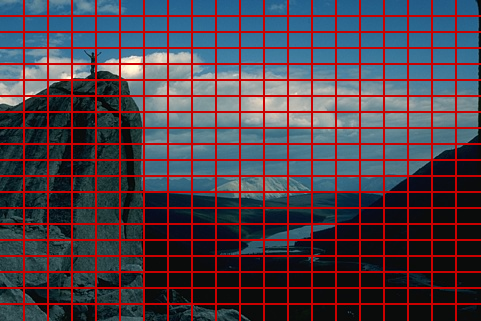
\includegraphics[scale=\scalefivebsd]{pictures/bsd-1-seeds-level-4}
	}
	\subfigure{
		\label{subfig:superpixel-segmentation-seeds-blocks-level-3}
		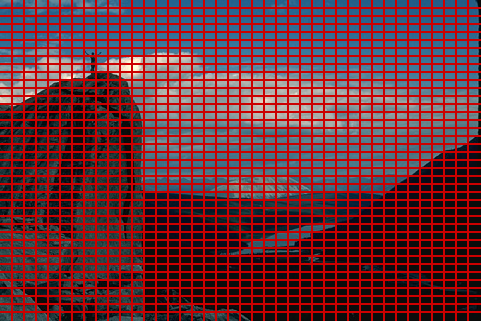
\includegraphics[scale=\scalefivebsd]{pictures/bsd-1-seeds-level-3}
	}
%	\subfigure[Blocks at level $l = 2$.]{
%		\label{subfig:superpixel-segmentation-seeds-blocks-level-2}
%		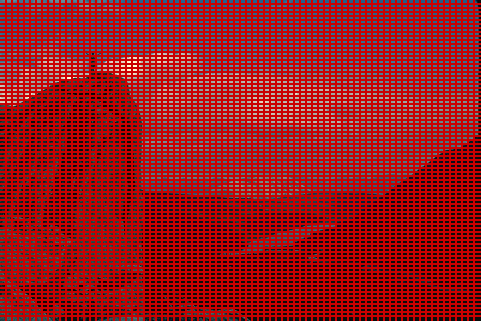
\includegraphics[scale=\scalethreebsd]{pictures/bsd-1-seeds-level-2}
%	}
	\subfigure{
		\label{subfig:superpixel-segmentation-seeds-blocks-after-3}
		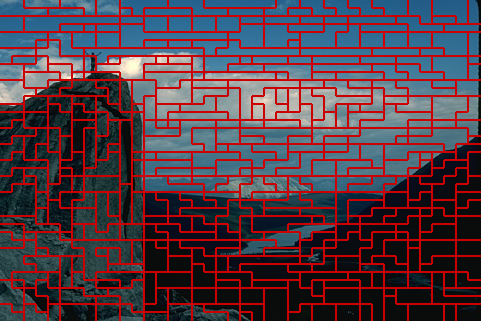
\includegraphics[scale=\scalefivebsd]{pictures/bsd-1-seeds-after-3}
	}
	\subfigure{
		\label{subfig:superpixel-segmentation-seeds-blocks-after-2}
		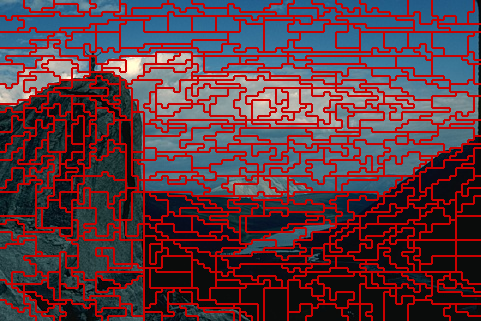
\includegraphics[scale=\scalefivebsd]{pictures/bsd-1-seeds-after-2}
	}
	\subfigure{
		\label{subfig:superpixel-segmentation-seeds-blocks-after-1}
		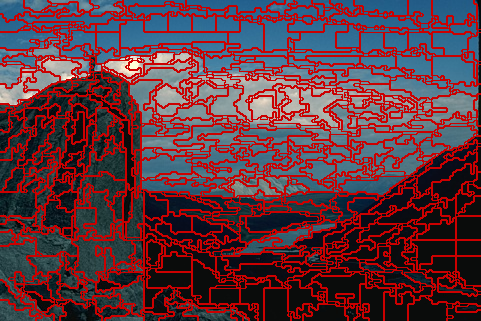
\includegraphics[scale=\scalefivebsd]{pictures/bsd-1-seeds-after-1}
	}
	\caption[An illustration of the block hierarchy used by \textbf{SEEDS} \cite{VanDenBerghBoixRoigCapitaniVanGool:2012} to exchange blocks between superpixels of an initial superpixel segmentation.]{Using $w^{(1)} = 3$, $h^{(1)} = 2$ and $L = 4$ which results in $400$ superpixels, from left to right: the block segmentation at level $l = 4$; the block segmentation at level $l = 3$; the superpixel segmentation after performing block updates at level $l = 3$; the superpixel segmentation after performing block updates at level $l = 2$ and the superpixel segmentation before performing pixel updates, that it after performing block updates at level $l = 1$.}
	\label{fig:superpixel-segmentation-seeds-blocks}
\end{figure}

As alternative to pixel updates based on color histograms, Van den Bergh \etal \cite{VanDenBerghBoixRoigCapitaniVanGool:2012} propose so called mean pixel updates. The similarity of pixel $x_n$ and superpixel $S_j$ is then expressed as euclidean distance in color space:
\begin{align}
	\label{eq:superpixel-segmentation-seeds-distance}
	d(x_n,S_j) = \| I(x_n) - I(S_j)\|_2.
\end{align}
Each pixel $x_n$ gets assigned to the superpixel minimizing the above distance, see algorithm \ref{algo:superpixel-segmentation-seeds-mean-pixel-updates}. We use \textbf{SEEDSmp} to refer to \textbf{SEEDS} using mean pixel updates.
\begin{algorithm}[t]
	\begin{algo}{SEEDS}{\label{algo:superpixel-segmentation-seeds-mean-pixel-updates}\qinput{color image $I$, initial superpixel segmentation $S$}\qoutput{superpixel segmentation $S$}}
		\qfor $k = 1$ \qto $K$\\
			initialize mean $I(S_k)$\qrof\\
		\qcom{Mean pixel updates:}\\
		\qfor $n = 1$ \qto $N$\\
			let $S_j$ be the superpixel $x_n$ belongs to\\
			\qif a neighboring pixel belongs to a different superpixel $S_k$\\
				\qthen\qif $d(x_n, S_k) < d(x_n, S_j)$\label{line:superpixel-segmentation-seeds-mean-pixel-criterion}\\
					\qthen $S_k$ \qlet $S_k \cup \{x_n\}$ and $S_j$ \qlet $S_j - \{x_n\}$\qfi\qfi\qrof\\
		\qreturn $S$
	\end{algo}
	\caption[As alternative to pixel updates as described in algorithm \ref{algo:superpixel-segmentation-seeds}, Van den Bergh \etal \cite{VanDenBerghBoixRoigVanGool:2013} propose mean pixel updates.]{As alternative to pixel updates as described in algorithm \ref{algo:superpixel-segmentation-seeds}, Van den Bergh \etal \cite{VanDenBerghBoixRoigVanGool:2013} propose mean pixel updates. This variant of \textbf{SEEDS} is referred to as \textbf{SEEDSmp}.}
	\label{fig:superpixel-segmentation-seeds-mean-pixel-updates}
\end{algorithm}

As compact and smooth superpixels may be preferable \cite{SchickFischerStiefelhagen:2012}, a smoothing term can be integrated into pixel updates. Therefore, we consider a local neighborhood around each pixel pair $(x_n,x_m)$ belonging to different superpixels $S_j$ and $S_k$, respectively. Let $N_1(x_n,x_m)$ denote the $3 \times 4$ or $4 \times 3$ neighborhood around the pixel pair $(x_n, x_m)$. %, see \ref{fig:superpixel-segmentation-seeds-smoothing}.
%\begin{figure}
%	\begin{tikzpicture}
%		\draw[dotted](-0.5,0) -- (0,0);\draw (0,0) -- (2,0);\draw[dotted](2,0) -- (2.5,0);
%		\draw[dotted](-0.5,0.5) -- (0,0.5);\draw (0,0.5) -- (2,0.5);\draw[dotted](2,0.5) -- (2.5,0.5);
%		\draw[dotted](0.5,-1) -- (0.5,-0.5);\draw (0.5,-0.5) -- (0.5,1);\draw[dotted](0.5,1) -- (0.5,1.5);
%		\draw[dotted](1,-1) -- (1,-0.5);\draw (1,-0.5) -- (1,1);\draw[dotted](1,1) -- (1,1.5);
%		\draw[dotted](1.5,-1) -- (1.5,-0.5);\draw (1.5,-0.5) -- (1.5,1);\draw[dotted](1.5,1) -- (1.5,1.5);
%	\end{tikzpicture}
%	\label{fig:superpixel-segmentation-seeds-smoothing}
%\end{figure}
If the number of pixels $N_{n,m,k}$ within $N_1(x_n,x_m)$ belonging to superpixel $S_k$ is greater than the number of pixels $N_{n,m,j}$ belonging to superpixel $S_j$, pixel $x_n$ is more likely to belong to superpixel $S_k$ as well\footnote{In practice, the pixel to be exchanged is not considered within the counts $N_{n,m,k}$ and $N_{n,m,j}$.} \cite{VanDenBerghBoixRoigCapitaniVanGool:2012}. The criterion for pixel updates given in line \ref{line:superpixel-segmentation-seeds-pixel-criterion} of algorithm \ref{algo:superpixel-segmentation-seeds} changes to
\begin{align}
	\label{eq:superpixle-segmentation-seeds-original-smoothing}
	N_{n,m,k} \cdot h_{S_k}(h(x_n)) > N_{n,m,j} \cdot h_{S_j}(h(x_n)).
\end{align}
For mean pixel updates as given in algorithm \ref{algo:superpixel-segmentation-seeds-mean-pixel-updates}, line \ref{line:superpixel-segmentation-seeds-mean-pixel-criterion} changes to
\begin{align}
	\label{eq:superpixle-segmentation-seeds-original-smoothing-mean}
	\frac{d(x_n,S_k)}{N_{n,m,k}} < \frac{d(x_n, S_j)}{N_{n,m,j}}.
\end{align}

An alternative smoothing term \cite{VanDenBerghBoixRoigVanGool:2013} uses the pixel coordinates to redefine the distance given in equation \eqref{eq:superpixel-segmentation-seeds-distance} as
\begin{align}
	\label{eq:superpixel-segmentation-seeds-spatial-smoothing}
	d(x_n,S_j) = \| I(x_n) - I(S_j)\|_2 + \beta\|x_n - \mu(S_j)\|_2.
\end{align}
where $\beta$ controls the compactness of the generated superpixels. Note that both smoothing terms can also be combined. With \textbf{SEEDSmp*} we refer to \textbf{SEEDS} using mean pixel updates and the alternative smoothing term of equation \eqref{eq:superpixel-segmentation-seeds-spatial-smoothing}.

\subsection{Complexity}
\label{subsection:superpixel-segmentation-seeds-complexity}

In the following we give a detailed analysis of the complexity of \textbf{SEEDS}. For initialization, we first run over all pixels to compute the corresponding histogram bins and then compute the histograms for level $l = 1$. Computing the histogram bins for each pixel can be done in $\mathcal{O}(N)$ operations using uniform binning or in $\mathcal{O}(3N + 255Q)$ operations using non-uniform binning based on integral channels\footnote{For each $8$-bit channel of the color image $I$, the corresponding integral channel represents an array where the $i^{\text{th}}$ entry, $0 \leq i \leq 255$, counts the number of pixels whose color in this channel is equal or smaller than $i$. Then, non-uniform binning chooses the bins such that approximately the same number of pixels fall in each bin.}. Together, this requires
\begin{align}
	\label{eq:superpixel-segmentation-seeds-complexity-initialization-1}
	3N + 255Q + \floor*{\frac{W}{w^{(1)}}} \cdot \floor*{\frac{H}{h^{(1)}}} \cdot w^{(1)} \cdot h^{(1)} = \mathcal{O}(4N + 255Q)
\end{align}
operations. The histograms at level $1 < l \leq L$ can be computed as the sum of the corresponding histograms at level $(l - 1)$: four blocks at level $(l - 1)$ form a block at level $l$. Then the initialization of the histograms for all levels $1 < l \leq L$ requires
\begin{align}
	\label{eq:superpixel-segmentation-seeds-complexity-initialization-l}
	\sum_{l = 2}^L 4\cdot \floor*{\frac{W}{w^{(l)}}} \cdot \floor*{\frac{H}{h^{(l)}}} \cdot Q \approx \sum_{l = 2}^L 4 \cdot \frac{N}{w^{(l)} h^{(l)}} \cdot Q
\end{align}
operations. Considering $w^{(1)} \geq 2$ and $h^{(1)} \geq 2$, equations \eqref{eq:superpixel-segmentation-seeds-complexity-initialization-1} and \eqref{eq:superpixel-segmentation-seeds-complexity-initialization-l} are at most linear in the number of pixels: $\mathcal{O}(4QN)$.

For block updates at level $1 \leq l < L$ we consider the worst case: each block has four neighbors belonging to different superpixels. Then, we need to compute the histogram intersection five times: four times for the neighboring superpixels, once for the current superpixel. Overall, for block updates at all levels $1 \leq l < L$, this results in
\begin{align}
	\label{eq:superpixel-segmentation-seeds-complexity-block-updates}
	\sum_{l = 1}^{L - 1} 5 \cdot \floor*{\frac{W}{w^{(l)}}} \cdot \floor*{\frac{H}{h^{(l)}}} \cdot Q \approx \sum_{l = 1}^{L - 1} 5 \cdot \frac{N}{w^{(l)}h^{(l)}} \cdot Q
\end{align}
operations. Hence, block updates at all levels $1 \leq l < L$ are linear in $N$ when considering the histogram size $Q$ to be a constant: $\mathcal{O}(5QN)$.

Considering pixel updates as in algorithm \ref{algo:superpixel-segmentation-seeds}, for each pixel we need to calculate the similarity to five different superpixels: $\mathcal{O}(5N)$ operations. Considering mean pixel updates as in algorithm \ref{algo:superpixel-segmentation-seeds-mean-pixel-updates}, computing the superpixel centers can be done in $\mathcal{O}(N + K)$ operations\footnote{In practice, for each superpixel $S_k$ the sums and the normalization needed to compute the means $I(S_k)$ and $\mu(S_k)$ are stored separately, resulting in $\mathcal{O}(N)$ operations for initialization.}. Further, in the worst case, $\mathcal{O}(5N)$ operations are necessary to perform mean pixel updates.

Overall, the algorithm has linear runtime in the number of pixels. However, for block updates, the number of histogram bins plays an important role. In addition, both block and pixel updates are in practice iterated more than once, such that the number of iterations $T$ influences the runtime as well: $\mathcal{O}(QTN)$. While this describes the worst case, we note that in practice, the runtime is also influenced by the number of levels $L$ and the block size $w^{(1)} \times h^{(1)}$.

\subsection{Theoretical Background}

We follow \cite{VanDenBerghBoixRoigCapitaniVanGool:2012} to derive the energy which Van den Bergh \etal aim to maximize using algorithm~\ref{algo:superpixel-segmentation-seeds}. The energy comprises a color term $H(S)$ and a smoothing term $B(S)$:
\begin{align}
	\label{eq:superpixel-segmentation-seeds-objective-function}
	E(S) = H(S) + \lambda B(S).
\end{align}
where $\lambda$ is a balancing parameter. In practice, $\lambda$ is not adaptable as the smoothing term introduced in equation \eqref{eq:superpixle-segmentation-seeds-original-smoothing} does not allow to adapt its importance.

The color term favors superpixels with color histograms concentrated in a single bin. Therefore, a color term of the form
\begin{align}
	\label{eq:superpixel-segmentation-seeds-color-term}
	H(S) = \sum_{S_j \in S} \sum_{q = 1} ^Q h_{S_j}(q)^2
\end{align}
is used. As of equation \eqref{eq:superpixel-segmentation-seeds-color-term}, $H(S)$ reaches its maximum if and only if each superpixel histogram is concentrated in a single bin \cite{VanDenBerghBoixRoigCapitaniVanGool:2012}. As alternative, Van den Bergh \etal refer to an entropy based color term\footnote{That is, $H(S) = - \sum_{S_j \in S} \sum_{q = 1} ^Q h_{S_j}(q) \log(h_{S_j}(q))$ where the histogram $h_{S_j}$ is interpreted as discrete probability distribution.}. Another possible color term is given by
\begin{align}
	H(S) = \sum_{S_j \in S} \max_q \{h_{S_j}(q)\},
\end{align}
favoring histograms concentrated in a single bin as well.

The boundary term is based on superpixel histograms. For each pixel $x_n$, the corresponding superpixel histogram $g_{x_n}$ counts the number of pixels $x_m \in N_R(x_n)$ belonging to each superpixel $1 \leq k \leq K$. Then, the boundary term is given by
\begin{align}
	B(S) = \sum_{n = 1}^N \sum_{k = 1} ^K g_{x_n}(k)^2.
\end{align}
This boundary term favors regular superpixels with smooth borders: When considering the superpixel histograms of all pixels within a specific superpixel, the superpixel histograms of pixels lying at the border will never be concentrated in one bin. However, with a more compact form of the superpixel, more pixels will have a uniformly labeled neighborhood, maximizing $B(S)$ \cite{VanDenBerghBoixRoigCapitaniVanGool:2012}.

To implement a hill climbing algorithm maximizing the energy $E(S)$, Van den Bergh \etal proof the following propositions:
\begin{prop}
	\label{prop:superpixel-segmentation-seeds-prop-1}
	Let $S_j$, $S_k$ be superpixels similar in size, and the size of block $B_i^{(l)} \subseteq S_j$ be much smaller: $|B_i^{(l)}| \ll |S_j| \approx |S_k|$. Let $S$ denote the current superpixel segmentation and $S_p$ denote the proposed superpixel segmentation where block $B_i^{(l)}$ is moved to superpixel $S_k$. If the color histogram $h_{B_i^{(l)}}$ is concentrated in one bin, it holds:
	\begin{align}
		\cap (h_{B_i^{(l)}}, h_{S_k}) \geq \cap (h_{B_i^{(l)}}, h_{S_j - B_i^{(l)}}) \Leftrightarrow H(S_p) \geq H(S)
	\end{align}
	where $h_{S_j - B_i^{(l)}}$ is the color histogram computed over the pixels in $S_j - B_i^{(l)}$.
\end{prop}
\begin{prop}
	\label{prop:superpixel-segmentation-seeds-prop-2}
	Let $x_n$ be a pixel belonging to superpixel $S_j$. Let $S$ denote the current superpixel segmentation and $S_p$ denote the proposed superpixel segmentation where $x_n$ is moved to superpixel $S_k$. Further, let $M_{x_n}$ be the set of all pixels $x_m$ for which $x_n \in N_R(x_m)$, then it holds:
	\begin{align}
		\sum_{x_m \in M_{x_n}} (g_{x_m}(k) + 1) \geq \sum_{x_m \in M_{x_n}} g_{x_m}(j) \Leftrightarrow G(S_p) \geq G(S).
	\end{align}
\end{prop}
\noindent Algorithm \ref{algo:superpixel-segmentation-seeds} is intended to maximize $E(S)$ via hill climbing: In each step, a new superpixel segmentation is proposed by exchanging blocks or pixels and the proposed superpixels segmentation is accepted if the energy increases.

\subsection{Discussion}

Although the implementation provided by Van den Bergh \etal performs well, the implementation lacks relation to the theoretical background discussed in the previous section. Firstly, proposition~\ref{prop:superpixel-segmentation-seeds-prop-1} assumes the superpixel sizes to be comparable and the histogram $h_{B_i^{(l)}}$ to be concentrated in a single bin. Arguing that this holds in 93\% of the cases \cite{VanDenBerghBoixRoigCapitaniVanGool:2012}, this can merely be seen as heuristic rather than mathematical accurate. Secondly, our experiments show that the energy given in equation \eqref{eq:superpixel-segmentation-seeds-objective-function} is unsuited for superpixel segmentation in the first place. Even though, an implementation directly maximizing $E(S)$ through hill climbing may be inefficient, figure \ref{fig:superpixel-segmentation-seeds-objective-function} presents superpixel segmentations obtained from a naive implementation.
\begin{figure}[t]
	\centering
	\subfigure{
		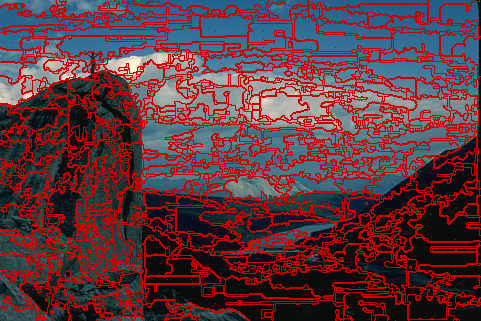
\includegraphics[scale=\scalefivebsd]{pictures/bsd-1-seeds-direct}
	}
	\subfigure{
		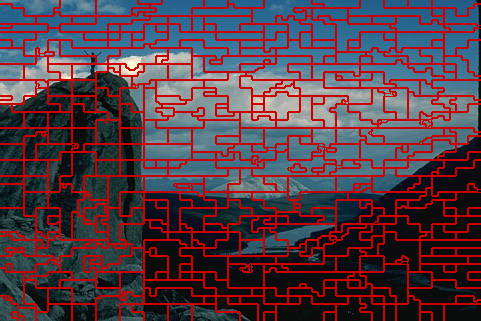
\includegraphics[scale=\scalefivebsd]{pictures/bsd-1-seeds-direct-after-1}
	}
	\subfigure{
		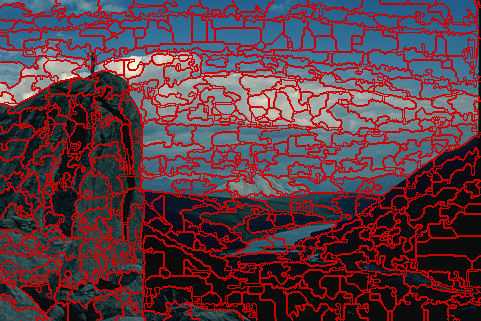
\includegraphics[scale=\scalefivebsd]{pictures/bsd-1-seeds-direct-original-pixels}
	}
	\caption[Superpixel segmentations generated by directly maximizing the energy proposed in \cite{VanDenBerghBoixRoigCapitaniVanGool:2012}.]{An illustration of the poor superpixel segmentations obtained by directly maximizing the proposed energy $E(S)$ given by equation \eqref{eq:superpixel-segmentation-seeds-color-term}. From left to right: the superpixel segmentation obtained after maximizing $E(S)$ directly using both block updates as well as pixel updates; the superpixel segmentation obtained after performing block updates at level $l = 1$ to directly maximize the energy $E(S)$; and the superpixel segmentation obtained after using block updates to optimize the energy $E(S)$ directly while using the pixel updates described in algorithm \ref{algo:superpixel-segmentation-seeds}.}
	\label{fig:superpixel-segmentation-seeds-objective-function}
\end{figure}
These experiments indicate that the idea of color histograms being concentrated in a single bin has to be relaxed in order to obtain proper superpixel segmentations. Thirdly, considering the smoothing term of the energy in equation \eqref{eq:superpixel-segmentation-seeds-objective-function}, the weight $\lambda$ cannot be adapted. Although this could be fixed by adapting equations \eqref{eq:superpixle-segmentation-seeds-original-smoothing} and \eqref{eq:superpixle-segmentation-seeds-original-smoothing-mean}, our experiments indicate that using the alternative smoothing term of equation \eqref{eq:superpixel-segmentation-seeds-spatial-smoothing} results in more compact and regular superpixels. Furthermore, mean pixel updates which are reported to give superior performance \cite{VanDenBerghBoixRoigVanGool:2013} do not conform to the theoretical background introduced in the previous section.
\begin{figure}[b]
	\centering
	\subfigure{
		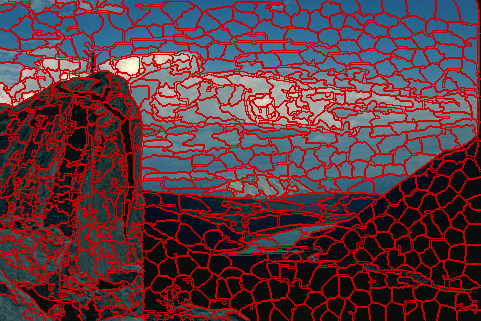
\includegraphics[scale=\scalefivebsd]{pictures/bsd-1-reseedssm}
	}
	\subfigure{
		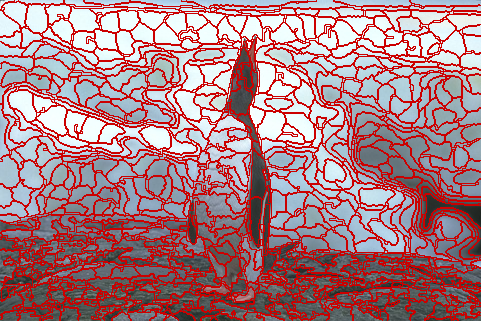
\includegraphics[scale=\scalefivebsd]{pictures/bsd-2-reseedssm}
	}
	\subfigure{
		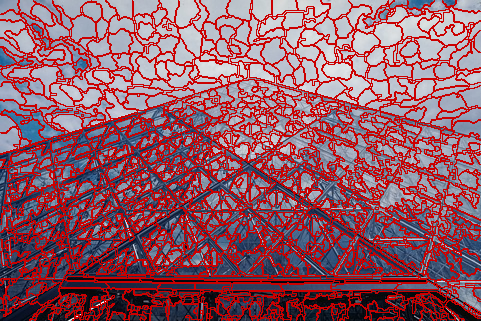
\includegraphics[scale=\scalefivebsd]{pictures/bsd-3-reseedssm}
	}
	\subfigure{
		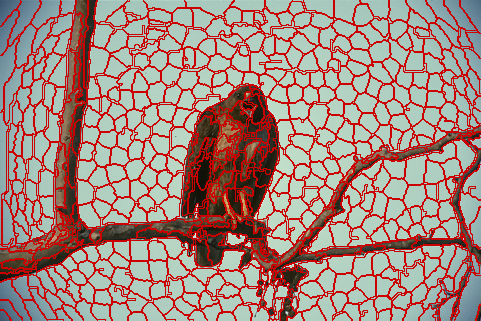
\includegraphics[scale=\scalefivebsd]{pictures/bsd-4-reseedssm}
	}
	\subfigure{
		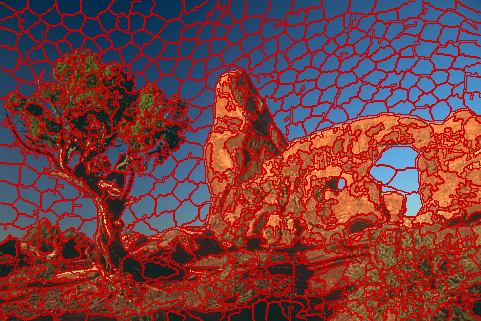
\includegraphics[scale=\scalefivebsd]{pictures/bsd-5-reseedssm}
	}
	\caption[Superpixel segmentations obtained from our implementation of \textbf{SEEDS} \cite{VanDenBerghBoixRoigCapitaniVanGool:2012} using mean pixel updates and the alternative smoothing term of equation \eqref{eq:superpixel-segmentation-seeds-spatial-smoothing}.]{The running examples oversegmented into exactly $600$ superpixels using our implementation of \textbf{SEEDS} using mean pixel updates and the alternative smoothing term of equation \eqref{eq:superpixel-segmentation-seeds-spatial-smoothing} which we refer to as \textbf{SEEDSmp*}. Further examples can be found in section \ref{subsection:evaluation-comparison-qualitative} and appendix \ref{chapter:appendix-evaluation}.}
	\label{fig:superpixel-segmentation-seeds-results}
\end{figure}
Overall, figure \ref{fig:superpixel-segmentation-seeds-results} shows the running examples oversegmented using our implementation with mean pixel updates as well as the alternative smoothing term of equation \eqref{eq:superpixel-segmentation-seeds-spatial-smoothing}. In conclusion, we find the theoretical background of \textbf{SEEDS} as provided by Van den Bergh \etal \cite{VanDenBerghBoixRoigCapitaniVanGool:2012} unsuited in the light of the provided implementation and our experiments. However, a novel formulation of \textbf{SEEDS} lies not within the scope of this thesis.

\subsection{Implementation Details}

Our implementation of \textbf{SEEDS} closely follows algorithm \ref{algo:superpixel-segmentation-seeds}. The histograms are pre-computed for all blocks across all levels. This can be done efficiently by accumulating histograms of level $(l - 1)$ to form the histograms in level $1 < l \leq L$. The original implementation, as well as our implementation, both use non-uniform binning, that is the bin size is adapted to the colors present within the image. Then, the histograms only need to be updated after exchanging blocks or pixels. When using mean pixel updates as in algorithm \ref{algo:superpixel-segmentation-seeds-mean-pixel-updates}, the superpixel centers need to be computed just before starting pixel updates. In practice the individual terms of equation \eqref{eq:superpixel-segmentation-seeds-spatial-smoothing} can also be normalized in order to choose the weighting parameter $\beta$ more easily.

\section{SLIC}
\label{section:superpixel-segmentation-slic}

\textbf{SLIC} is a gradient ascent method growing superpixels from initial superpixel centers using color similarity and spatial proximity. In particular, \textbf{SLIC} performs local $K$-means clustering where the search space for each superpixel is restricted to a local neighborhood around its center. The approach is easily implemented and adapted to custom needs. In addition, it can naturally be extended to depth or video data and is commonly used for comparison. We revisit the algorithm in detail and give a brief discussion.

% \textbf{SLIC} is a gradient ascent approach, as well, and comparable to a local $K$-means clustering (\eg see \cite{Bishop:2006} for details on $K$-means clustering). It is fast because the search space for each superpixel is limited to a local neighborhood. We revisit the algorithm before giving a short discussion. For this thesis, \textbf{SLIC} is of interest as it implements a superpixel algorithm easily extendable to using depth information (see chapter \ref{chapter:superpixel-segmentation-depth}) and as it is commonly used as baseline.

\subsection{Algorithm}

The algorithm can be described as local $K$-means clustering in a five dimensional space comprising pixel coordinates and color \cite{AchantaShajiSmithLucchiFuaSuesstrunk:2010}, see algorithm \ref{algo:superpixel-segmentation-slic}.
\begin{algorithm}[t!]
	\begin{algo}{SLIC}{\label{algo:superpixel-segmentation-slic}\qinput{color image $I$, number of superpixels $K$}\qoutput{superpixel segmentation $S$}}
		initialize superpixel centers on a regular grid with step size $R$\\
		move centers to low-gradient magnitude positions\\
		\qrepeat\\
			\qfor $k = 1$ \qto $K$\\
				\qforeach pixel $x_n$ in a $2R \times 2R$ neighborhood around $\mu(S_k)$\\
					\qif $x_n$ is unassigned\\
						\qthen $S_k$ \qlet $S_k \cup \{x_n\}$\qfi\\
					\qelseif $d(x_n, S_k) < d(x_n, S_{s(x_n)})$\\
						\qthen $S_k$ \qlet $S_k \cup \{x_n\}$ and $S_{s(x_n)}$ \qlet $S_{s(x_n)} - \{x_n\}$\qfi\qrof\qrof
		\quntil nothing changes \qcom{or maximum number of iterations reached.}\\
		enforce connectivity\\
		\qreturn $S$
	\end{algo}
	\caption[The basic algorithm of \textbf{SLIC} \cite{AchantaShajiSmithLucchiFuaSuesstrunk:2010}.]{\textbf{SLIC} is implemented as local $K$-means clustering. Here, local means that for each superpixel only pixels in a $2R \times 2R$ window around the superpixel's center are of interest. After clustering, \textbf{SLIC} needs to enforce connectivity.}
	\label{fig:superpixel-segmentation-slic-algorithm}
\end{algorithm}
The superpixel centers are initialized on a regular grid with step size $R$. In practice, the centers are then moved to locations with low gradient magnitude to avoid placing superpixel centers at strong edges. The step size of the regular grid can be computed as
\begin{align}
	R = \floor*{\frac{WH}{K}}.
\end{align}
Then, each pixel $x_n$ gets assigned to the nearest superpixel with respect to the following distance:
\begin{align}
	\label{eq:superpixel-segmentation-slic-distance}
	d(x_n, S_j) = \|I(x_n) - I(S_j)\|_2 + \frac{\beta}{R} \|x_n - \mu(S_j)\|_2
\end{align}
where $\beta$ is a parameter controlling the compactness. However, in contrast to classical $K$-means clustering, for each superpixel only pixels in a $2R \times 2R$ neighborhood around the superpixel's center are of interest. Afterwards, the superpixel centers are updated according to the new assignment. This procedure is iterated until convergence or for a maximum number of $T$ iterations. Finally, superpixels do not necessarily represent connected components such that \textbf{SLIC} needs to enforce connectivity after clustering.

\subsection{Theoretical Background}

In general, $K$-means clustering minimizes an energy given by
\begin{align}
	\label{eq:superpixel-segmentation-slic-objective}
	E(S) = \sum_{S_j \in S} \sum_{n = 1}^N a_{n,j} d(x_n, S_j)^2
\end{align}
where $a_{n,j} = 1$ if and only if pixel $x_n$ is assigned to superpixel $S_j$, else $a_{n,j} = 0$. However, \textbf{SLIC} relaxes this energy in that the search space for each superpixel is restricted to a $2R \times 2R$ neighborhood around $\mu(S_j)$. Therefore, for fixed $\mu(S_j)$, the energy can be rewritten as
\begin{align}
	E(S) = \sum_{S_j \in S} \sum_{x_n \in N_{2R}(\mu(S_j))} a_{n,j} d(x_n, S_j)^2.
\end{align}
Additionally, the above energy is not minimized subject to the constraint that the superpixels $S_j$ are connected components. Therefore, the last step of enforcing connectivity may actually increase the energy.

\subsection{Complexity}

While classical $K$-means clustering has complexity $\mathcal{O}(NKT)$, \textbf{SLIC} runs linear in the number of pixels because of the restricted search space: For each superpixel, only pixels in a $2R \times 2R$ neighborhood around the superpixel's center are considered. Therefore, \textbf{SLIC} has complexity $\mathcal{O}(TN)$.

\subsection{Discussion}

One advantage of \textbf{SLIC} is its simplicity and efficiency \cite{AchantaShajiSmithLucchiFuaSuesstrunk:2012}. There are several implementations available: the original implementation by Achanta \etal \cite{AchantaShajiSmithLucchiFuaSuesstrunk:2010}, an implementation as part of the VLFeat Library \cite{VedaldiFulkerson:2008} and a parallel GPU implementation by Ren and Reid \cite{RenReid:2011}. Further, \textbf{SLIC} can easily be adapted by changing the distance in equation \eqref{eq:superpixel-segmentation-slic-distance}. For example, Schick \etal improve the balancing between color and spatial term by changing equation \eqref{eq:superpixel-segmentation-slic-distance} to
\begin{align}
	d(x_n, S_j) = (1 - \beta)\|I(x_n) - I(S_j)\|_2 + \frac{\beta}{R} \|x_n - \mu(S_j)\|_2.
\end{align}

On the other hand, \textbf{SLIC} only generates a valid superpixel segmentation after enforcing connectivity. This means, that the algorithm cannot be aborted after an arbitrary number of iterations. In addition, Van den Bergh \etal \cite{VanDenBerghBoixRoigVanGool:2013} report lower performance with more iterations which may be due to the generated ``stray labels'' \cite{VanDenBerghBoixRoigVanGool:2013} -- small groups of pixels not connected to their corresponding superpixel. This is also confirmed by Tang \etal \cite{DaiTangHuazhaFuXiaochunCao:2012} reporting only a small decrease in performance when using only $T = 1$ iteration. However, considering an approach similar to \textbf{VCCS} \cite{PaponAbramovSchoelerWoergoetter:2013} (see section \ref{section:superpixel-segmentation-depth-vccs}), breadth-first search could be used as basis for $K$-means clustering in order to avoid stray labels. To sum up, figure \ref{fig:superpixel-segmentation-slic-results} shows the running examples oversegmented using the original implementation of \textbf{SLIC}.
\begin{figure}[t]
	\centering
	\subfigure{
		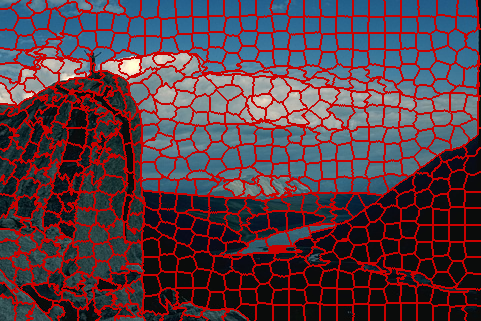
\includegraphics[scale=\scalefivebsd]{pictures/bsd-1-orislic}
	}
	\subfigure{
		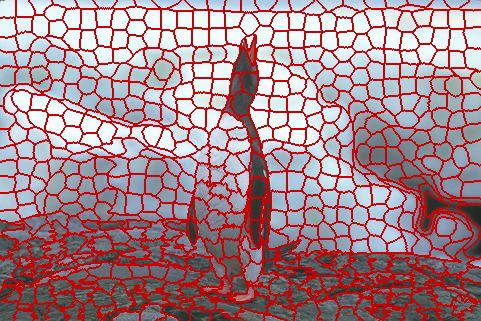
\includegraphics[scale=\scalefivebsd]{pictures/bsd-2-orislic}
	}
	\subfigure{
		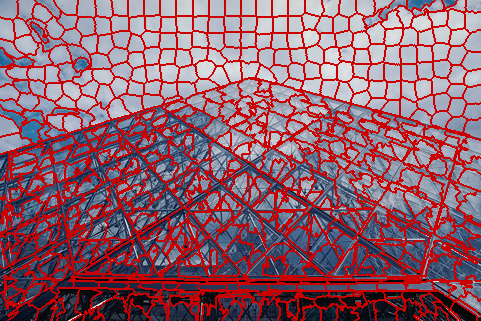
\includegraphics[scale=\scalefivebsd]{pictures/bsd-3-orislic}
	}
	\subfigure{
		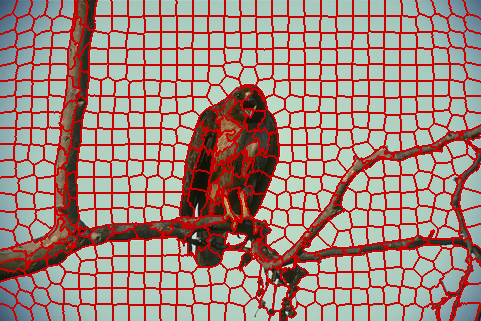
\includegraphics[scale=\scalefivebsd]{pictures/bsd-4-orislic}
	}
	\subfigure{
		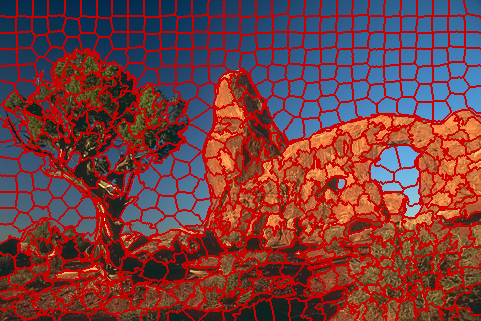
\includegraphics[scale=\scalefivebsd]{pictures/bsd-5-orislic}
	}
	\caption[Superpixel segmentations generated by the original implementation of \textbf{SLIC} \cite{AchantaShajiSmithLucchiFuaSuesstrunk:2012}.]{Superpixel segmentations with roughly $600$ superpixels of the running examples generated by the original implementation of \textbf{SLIC}. Further examples can be found in section \ref{subsection:evaluation-comparison-qualitative} and appendix~\ref{chapter:appendix-evaluation}.}
	\label{fig:superpixel-segmentation-slic-results}
\end{figure}
\chapter{Supervoxel Segmentation and Superpixel Segmentation using Depth}
\label{chapter:superpixel-segmentation-depth}

The focus of this thesis is the integration of depth information into \textbf{SEEDS} \cite{VanDenBerghBoixRoigCapitaniVanGool:2012} as we believe that depth may serve as additional cue to identify object boundaries and improve the generated superpixel segmentation. Some of the superpixel algorithms discussed in section \ref{section:related-work-superpixel-segmentation} can easily be extended to use depth information, for example \textbf{CRS} \cite{ConradMertzMester:2013} and \textbf{SLIC} \cite{AchantaShajiSmithLucchiFuaSuesstrunk:2010}. Graph based approaches can also be extended to use depth information by adapting the weights accordingly, for example \textbf{ERS} \cite{LiuTuzelRamalingamChellappa:2011} and \textbf{PB} \cite{ZhangHartleyMashfordBurn:2011}. An extension of \textbf{SLIC} based on depth is discussed in the following section. However, there are more sophisticated approaches available: \textbf{DASP} \cite{WeikersdorferGossowBeetz:2012} places the initial superpixel centers depending on the depth, and with \textbf{VCCS} \cite{PaponAbramovSchoelerWoergoetter:2013}, Papon \etal provide an approach able to oversegment point clouds. We revisit both approaches in detail as they will serve as additional baselines and present state-of-the-art algorithms using depth as an integral component.

\section{SLIC using Depth Information}
\label{section:superpixel-segmentation-depth-slic3d}

\textbf{SLIC} is built around a distance function $d(x_n, S_j)$ as defined in equation \eqref{eq:superpixel-segmentation-slic-distance}. As this distance already uses pixel coordinates, we can add an additional term to introduce depth:
\begin{align}
	\label{eq:supeprixel-segmentation-depth-slic3d-distance-depth}
	d(x_n, S_j) = \|I(x_n) - I(S_j)\|_2 + \frac{\beta}{R}\|x_n - \mu(S_j)\| + \gamma\|D(x_n) - D(S_j)\|_2
\end{align}
where $\gamma$ is an additional weighting term and $D: \ubar{W} \times \ubar{H} \rightarrow \mathbb{R}$ represents a depth image. The depth of a superpixel $S_j$ is defined as $D(S_j) = \frac{1}{|S_j|} \sum_{x_m \in S_i} D(x_m)$. This distance aims to discourage superpixels crossing boundaries including a difference in depth.

Instead of using pixel coordinates and depth as separate information, we can project the pixel coordinates $x_n$ into three-dimensional space to obtain the corresponding 3D point coordinates which we denote by $P(x_n) \in \mathbb{R}^3$. The distance in equation \eqref{eq:supeprixel-segmentation-depth-slic3d-distance-depth} changes to
\begin{align}
	\label{eq:superpixel-segmentation-depth-slic3d-distance}
	d(x_n, S_j) = \|I(x_i) - I(S_j)\|_2 + \beta \| P(x_n) - P(S_j) \|_2
\end{align}
with $P(S_j) = \frac{1}{|S_j|} \sum_{s_m \in S_j} P(x_m)$. Connectivity can still be enforced on the image plane. We implemented this variant of \textbf{SLIC}, in the following referred to as \textbf{SLIC3D}, as additional baseline.

\subsection{Discussion}

Because of \textbf{SLIC}'s good performance, we do not expect a significant increase in performance while slightly increasing the runtime due to the extended distance in equation~\eqref{eq:superpixel-segmentation-depth-slic3d-distance}. However, we are able to observe a visual difference in the generated superpixels as, depending on the value of $\beta$, \textbf{SLIC3D} enforces compactness within three dimensional space such that the superpixels appear to reflect the underlying three dimensional structure. Figure \ref{fig:superpixel-segmentation-slic3d-comparison} shows the generated superpixel segmentations of the running examples.
\begin{figure}[t]
	\centering
	\subfigure{
		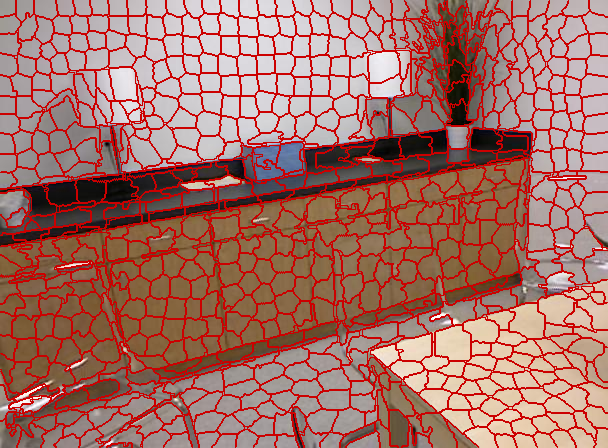
\includegraphics[scale=\scalefivenyu]{pictures/nyu-1-slic3d}
	}
	\subfigure{
		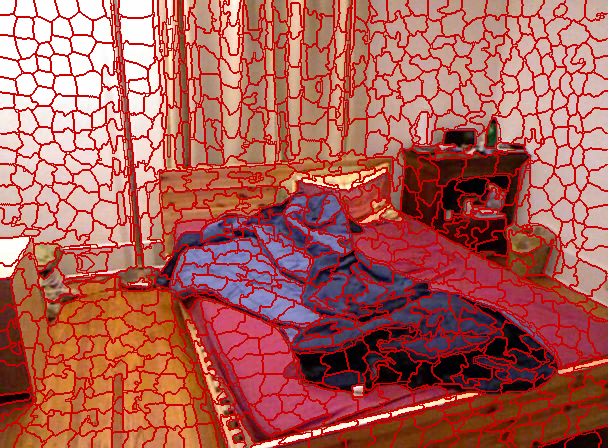
\includegraphics[scale=\scalefivenyu]{pictures/nyu-2-slic3d}
	}
	\subfigure{
		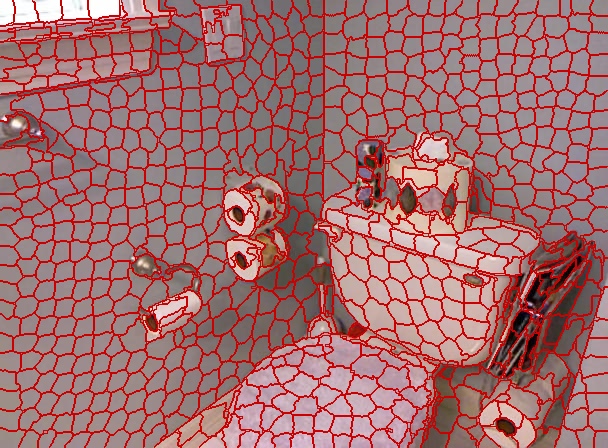
\includegraphics[scale=\scalefivenyu]{pictures/nyu-3-slic3d}
	}
	\subfigure{
		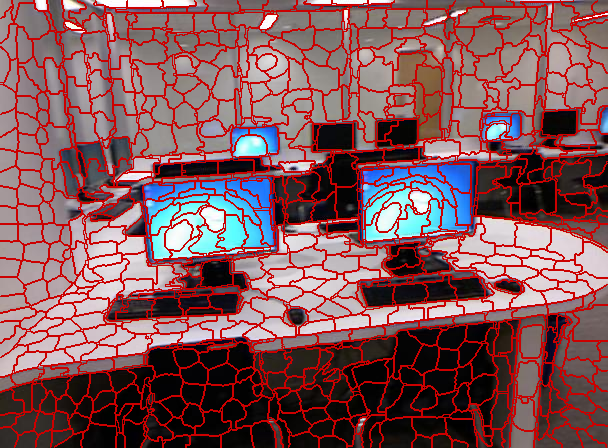
\includegraphics[scale=\scalefivenyu]{pictures/nyu-4-slic3d}
	}
	\subfigure{
		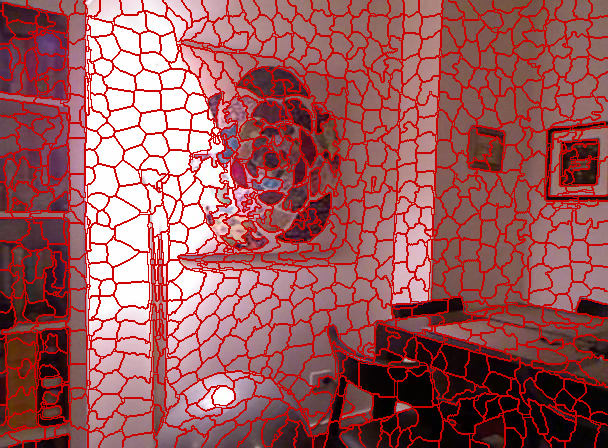
\includegraphics[scale=\scalefivenyu]{pictures/nyu-5-slic3d}
	}
	\caption[The running examples oversegmented using an extension of \textbf{SLIC} \cite{AchantaShajiSmithLucchiFuaSuesstrunk:2010} using depth information.]{Superpixel segmentations with roughly $840$ superpixels of the running examples generated using \textbf{SLIC3D}. Further examples can be found in section \ref{subsection:evaluation-comparison-qualitative} or appendix \ref{chapter:appendix-evaluation}.}
	\label{fig:superpixel-segmentation-slic3d-comparison}
\end{figure}

\section{DASP}
\label{section:superpixel-segmentation-dasp}

% TODO: add derivation of area.
% TODO: mention generalization of concept known as ASP (see GitHub)
The approach proposed by Weikersdorfer \etal \cite{WeikersdorferGossowBeetz:2012} is based on an important observation. Usually, we choose the number of superpixels such that we obtain superpixels comparable in size to the smallest objects we are interested in \cite{WeikersdorferGossowBeetz:2012}. Consequently, the density of superpixels is higher at surfaces farther away from the image plane \cite{WeikersdorferGossowBeetz:2012}, that is with increasing depth the superpixels get smaller on average. Nevertheless, we want the superpixels to be distributed uniformly on surfaces at any depth. This is achieved by defining a superpixel density on the depth image. We follow \cite{WeikersdorferGossowBeetz:2012} and consider a disk of radius $R$ centered at pixel $x_n$ in depth $D(x_n)$. Using the model of a pinhole camera \cite{ForsythPonce:2002}, the radius of this disk projected onto the image plane is given by
\begin{align}
	r(x_n) = \frac{f}{D(x_n)} R
\end{align}
where $f$ denotes the focal length of the camera. As noted in \cite{WeikersdorferGossowBeetz:2012}, this equation can only be applied in cases where the disk is parallel to the image plane. Otherwise, a projective transformation would be necessary which Weikersdorfer \etal approximate using an affine transformation. First, the gradient $\nabla D(x_n)$ of the depth image is estimated using finite differences. Then, the area of the projected disk can be expressed~as
\begin{align}
	A(x_n) = \frac{r(x_n)^2\pi}{\sqrt{\|\nabla D(x_n)\|_2^2 + 1}}
\end{align}
and the superpixel density at pixel $x_n$ is proportional to $\frac{1}{A(x_n)}$. A detailed derivation can be found in \cite{Weikersdorfer:2014}. In practice, the provided implementation of \textbf{DASP} offers several methods to sample the initial superpixel centers from this density, one of which is given by random sampling, summarized in algorithm \ref{algo:superpixel-segmentation-depth-dasp-random}.
\begin{algorithm}[t!]
	\begin{algo}{DASP (sed sampling)}{\label{algo:superpixel-segmentation-depth-dasp-random}\qinput{color image $I$, density $p(x_n) \propto \frac{1}{A(x_n)}$}\qoutput{superpixel centers $\mu(S) = \{\mu(S_1),\ldots,\mu(S_K)\}$}}
		initialize $\mu(S) = \emptyset$\\
		\qfor $n = 1$ \qto $N$\\
			$r$ \qlet $random([0, 1])$\\
			\qif $r < p(x_n)$\\
				\qthen $\mu(S)$ \qlet  $\mu(S) \cup \{x_n\}$\qfi\qrof\\
		\qreturn $\mu(S)$
	\end{algo}
	\caption[\textbf{DASP} \cite{WeikersdorferGossowBeetz:2012} randomly samples the initial superpixel centers from a custom density based on depth information.]{The easiest way to sample superpixel centers form the superpixel density $p(x_n)$ is given by random sampling. For each pixel, a number in the range $[0,1]$ is randomly chosen and compared to the probability $p(x_n)$ of $x_n$ being an initial superpixel center. For details how the desired number of superpixels is met we refer to the implementation\footnote{Available at \url{https://github.com/Danvil/dasp}.}.}
	\label{fig:superpixel-segmentation-depth-dasp-random}
\end{algorithm}
Note that the above mechanism can also be applied to custom densities or densities based on different information, see \cite{Weikersdorfer:2014} for details.

Similar to \textbf{SLIC}, the algorithm alternates between the assignment step where each pixel is assigned to the nearest superpixel and the update step where the superpixel centers are updated. The used distance is given by
\begin{align}
	\label{eq:superpixel-segmentation-depth-dasp-distance}
	d(x_n, S_j) = \|I(x_n) - I(S_j)\|_2 + \beta\|P(x_n) - P(S_j)\|_2 + \gamma \left(1 - N(x_n)^T N(S_j)\right)
\end{align}
where $\beta$ and $\gamma$ are parameters weighting the corresponding terms and $N(x_n)$ denotes the normal corresponding to pixel $x_n$ which we assume to be normalized. Again, we use $N(S_j) = \frac{1}{|S_j|} \sum_{x_m \in S_j} N(x_m)$ and the normals are estimated using depth gradients. The term $N(x_n)^T N(S_j)$ represents the cosine of the angle between the normals $N(x_n)$ and $N(S_j)$. Here, the intuition is that pixel $x_n$ and superpixel $S_j$ lie on the same planar surface if this angle is small. On the other hand, the cosine of this angle reaches zero if the normals are orthogonal to each other.

\subsection{Discussion}

In contrast to \textbf{SLIC3D}, the approach presented above not only uses 3D point coordinates and normal information but also adapts the size of superpixels according to the given depth. This way we expect to get performance comparable to superpixel algorithms like \textbf{SLIC} and \textbf{SEEDS}, however, with a lower number of superpixels. Additionally, by using normal information, \textbf{DASP} may recognize additional boundaries not apparent when using color and 3D point coordinates only. Figure \ref{fig:superpixel-segmentation-depth-dasp-comparison} shows the running examples oversegmented using \textbf{DASP}.
\begin{figure}[t]
	\centering
	\subfigure{
		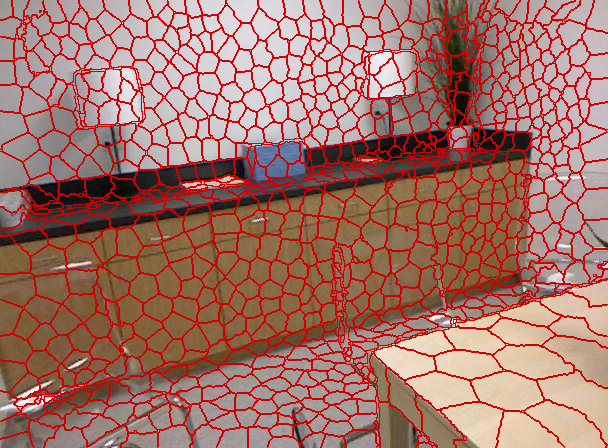
\includegraphics[scale=\scalefivenyu]{pictures/nyu-1-dasp}
	}
	\subfigure{
		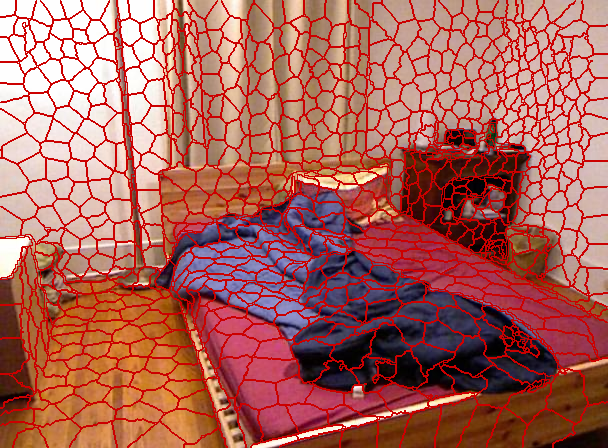
\includegraphics[scale=\scalefivenyu]{pictures/nyu-2-dasp}
	}
	\subfigure{
		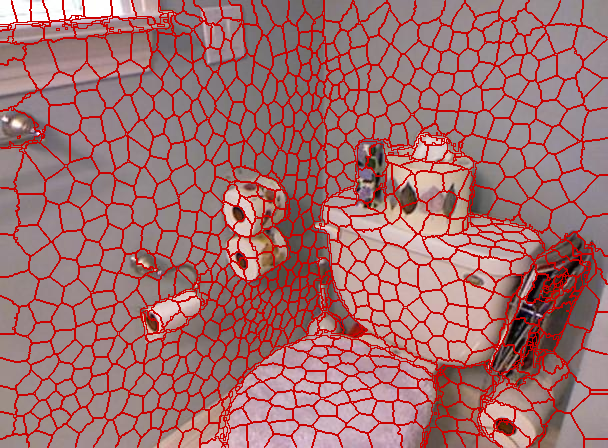
\includegraphics[scale=\scalefivenyu]{pictures/nyu-3-dasp}
	}
	\subfigure{
		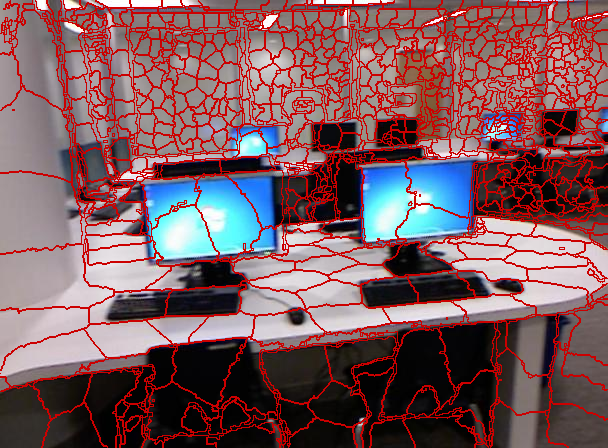
\includegraphics[scale=\scalefivenyu]{pictures/nyu-4-dasp}
	}
	\subfigure{
		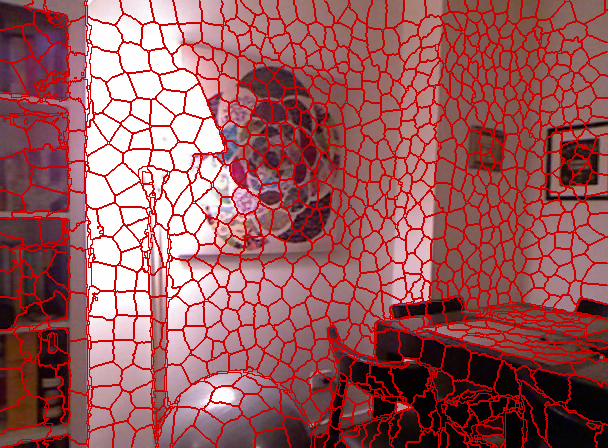
\includegraphics[scale=\scalefivenyu]{pictures/nyu-5-dasp}
	}
	\caption[Superpixel segmentations of the running examples generated by \textbf{DASP} \cite{WeikersdorferGossowBeetz:2012}.]{Superpixel segmentations with roughly $840$ superpixels of the running examples generated by \textbf{DASP}. Further examples are available in section \ref{subsection:evaluation-comparison-qualitative} and appendix \ref{chapter:appendix-evaluation}.}
	\label{fig:superpixel-segmentation-depth-dasp-comparison}
\end{figure}

\section{VCCS}
\label{section:superpixel-segmentation-depth-vccs}

% TODO: introduce background on point clouds!
% TODO: introduce different notion of S_i (set of 3D points now).
Although \textbf{VCCS} may be applied to arbitrary point clouds as for example generated from multiple RGB-D cameras or laser scans \cite{PaponAbramovSchoelerWoergoetter:2013}, we assume the point cloud to be created from a single image with corresponding depth image. Note that this results in a dense and ordered point cloud\footnote{That is, the points are accessible by their pixel coordinates within a two dimensional array.}. The point cloud is voxelized using a given voxel resolution $R_v$ such that an $26$-adjacency graph can be defined, see \cite{Rusu:2009} for details.

The idea of \textbf{VCCS} is similar to \textbf{SLIC} in that it performs local $K$-means clustering within the voxelized point cloud. However, \textbf{VCCS} ensures connectivity by applying breadth-first search as basis for clustering. After placing supervoxel centers at a regular grid with step size\footnote{Note that this step size is applied in three dimensional space.} $R$, also called supervoxel resolution\footnote{Actually, Papon \etal \cite{PaponAbramovSchoelerWoergoetter:2013} call $R$ seed resolution where a seed corresponds to a supervoxel center. This naming is often used for superpixel centers as well \cite{AchantaShajiSmithLucchiFuaSuesstrunk:2010}.}, we first need to remove supervoxel centers which have no voxels in their immediate neighborhood. If a given supervoxel center would lie on a planar surface, then the following equation yields the number of voxels within a specified search radius $R_s$:
\begin{align}
	\frac{R_s^2 \pi}{R_v^2}
\end{align}
where $R_v^2$ describes the ground area of a single voxel. All supervoxel centers having less voxels in the sphere of radius $R_s$ are discarded (see the implementation in the Point Cloud Library\footnote{The Point Cloud Library, implemented in C++, is mainly aimed to provide state-of-the-art computer vision algorithms running on point clouds: \url{http://pointclouds.org/}.} \cite{RusuCousins:2011} for details). Afterwards, the supervoxel centers are moved to low gradient magnitude positions similar to \textbf{SLIC}.% Furthermore, the supervoxel centers are moved to the mean position within a local neighborhood.

According to \cite{PaponAbramovSchoelerWoergoetter:2013}, \textbf{VCCS} performs clustering in a $39$ dimensional space comprising color, 3D point coordinates and Fast Point Feature Histograms \cite{RusuBlodowBeetz:2009}, short FPFH. However, the implementation available as part of the Point Cloud Library suggests that instead of FPFH features, point normals are used. Additionally, our experiments suggest that using FPFH features is quite expensive regarding runtime. Thus, we focus on the version as provided by the Point Cloud Library. The used distance function is given by
\begin{align}
	\label{eq:superpixel-segmentation-depth-vccs-distance}
	d(x_n, S_j) = \|I(x_n) - I(S_j)\|_2 + \beta\|P(x_n) - P(S_j)\|_2 + \gamma \left(1 - N(x_n)^T N(S_j)\right)
\end{align}
where $\beta$ and $\gamma$ are parameters weighting the spatial and normal terms.

\begin{algorithm}[t]
	\begin{algo}{VCCS}{\label{algo:superpixel-segmentation-depth-vccs}\qinput{voxelized point cloud, supervoxel resolution $R$, search radius $R_s$}\qoutput{superpixel segmentation $S$}}
		place supervoxel centers on a regular grid with step size $R$\\
		discard unnecessary supervoxel centers based on the search radius $R_s$\\		
		move supervoxel centers to low gradient magnitude positions\\
		%\qcom{Eventually, move supervoxel centers to mean position within local neighborhood}\\
		\qfor $t = 1$ \qto $T$ \qcom{$T$ is the maximum depth.}\\
			\qfor $k = 1$ \qto $K$\\
				perform one step breadth first search for supervoxel $S_k$\\
				update supervoxel center\qrof\qrof\\
		derive superpixel segmentation $S$ by backprojecting the supervoxels\\
		\qreturn $S$
	\end{algo}
	\caption[The supervoxel algorithm \textbf{VCCS} \cite{PaponAbramovSchoelerWoergoetter:2013}.]{\textbf{VCCS} uses $K$-means clustering based on breadth-first search beginning at the supervoxel centers to assign each voxel to a supervoxel. This way, \textbf{VCCS} ensures that the supervoxels represent connected components within the $26$-adjacency graph derived from the voxelized point cloud. The below algorithm can easily be adapted to return a supervoxel segmentation instead of a superpixel segmentation.}
	\label{fig:superpixel-segmentation-depth-vccs-breadth-first}
\end{algorithm}
The clustering process is different to the local $K$-means clustering used by \textbf{SLIC} in that it implements a breadth-first search beginning at the supervoxel centers. As for \textbf{SLIC}, the pixels being of interest for a particular supervoxel $S_j$ are limited by the maximum depth $T$ of the breadth-first search. In practice, the maximum depth $T$ is set to
\begin{align}
	T = 1.8 \cdot \frac{R}{R_v}.
\end{align}
\textbf{VCCS} is, slightly simplified, described in algorithm \ref{algo:superpixel-segmentation-depth-vccs}.

\subsection{Discussion}

While the approaches discussed in section \ref{section:superpixel-segmentation-depth-slic3d} and \ref{section:superpixel-segmentation-dasp} generate superpixel segmentations using depth as additional cue, \textbf{VCCS} creates supervoxels directly in three dimensional space. This is advantageous when considering input from multiple RGB-D cameras describing the same scene or laser scans \cite{PaponAbramovSchoelerWoergoetter:2013}. Furthermore, the algorithm can be applied to unordered point clouds. Additionally, in contrast to \textbf{SLIC}, \textbf{VCCS} does not need to enforce connectivity afterwards.

On the other hand, being dependent on a point cloud can also have major disadvantages when aiming to oversegment images for which depth information is available separately. For example \textbf{SLIC3D} or \textbf{DASP} can easily be applied to images with incomplete depth information by falling back to a color only mode. As we discuss in chapter \ref{chapter:datasets}, this is often the case when grabbing raw images from RGB-D cameras like the Microsoft Kinect. In such a case we are not able to generate a complete point cloud such that \textbf{VCCS} cannot be applied to the whole image. However, note that these considerations differ depending on the application. Furthermore, we note that the comparison of superpixel algorithms with supervoxel algorithms is difficult by design.

As the distance used for clustering is equal to the distance used by \textbf{DASP}, we cannot expect to observe increased performance due to different features. However, in contrast to \textbf{SLIC3D} and \textbf{DASP}, \textbf{VCCS} avoids stray labels and respects the underlying three dimensional surface directly by oversegmenting a point cloud in the form of a $26$-adjacency graph. Although \textbf{SLIC3D} and \textbf{DASP} would be able to detect boundaries within the depth image, depending on the parameter $\beta$, these boundaries can also be ignored. Due to the breadth-first search utilized by \textbf{VCCS} such cases are handled automatically. Overall, we expect improved performance for a lower number of superpixels when compared to other approaches. \textbf{VCCS} applied to the running examples is shown in figure \ref{fig:superpixel-segmentation-depth-vccs-comparison}.

% Beneath the above difficulties, there are further aspects to discuss concerning the algorithm and its implementation. First of all, \textbf{VCCS} is available as part of the Point Cloud Library \cite{Rusu:2009}. However, the implementation differs from the proposed algorithm in \cite{PaponAbramovSchoelerWoergoetter:2013} in that FPFH features are not used for clustering. Instead, a distance similar to the one used by \textbf{DASP} is utilized. Nevertheless, \textbf{VCCS} has the advantage that it avoids stray labels as known from \textbf{SLIC}. Overall, we expect not to get increased performance because of the different features used but rather because of a different initialization of the supervoxel centers and clustering directly within a point cloud. As using \textbf{DASP} this may result in performance comparable to superpixel algorithms not using depth information while generating less supervoxels. \textbf{VCCS} applied to our running examples can be seen in figure \ref{fig:superpixel-segmentation-depth-vccs-comparison}.
\begin{figure}[t]
	\centering
	\subfigure{
		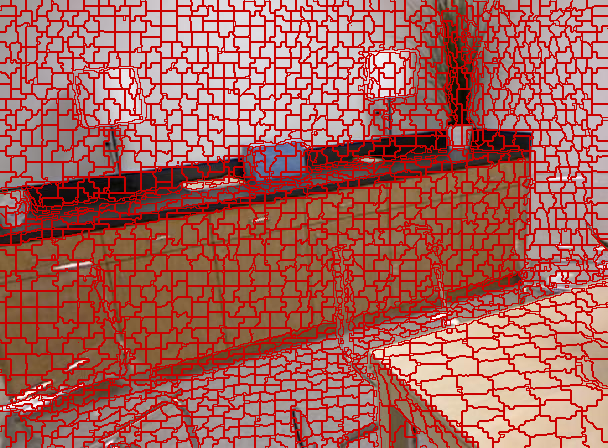
\includegraphics[scale=\scalefivenyu]{pictures/nyu-1-vccs}
	}
	\subfigure{
		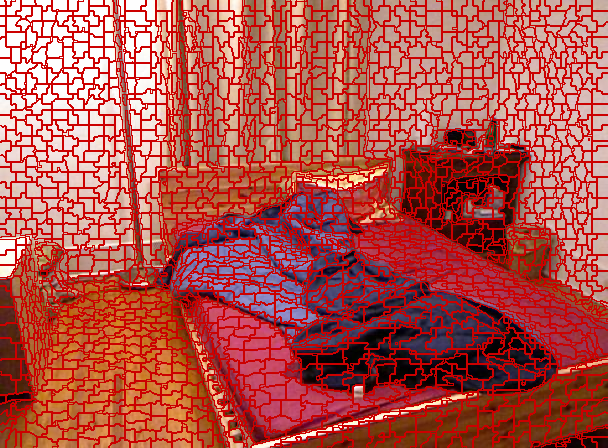
\includegraphics[scale=\scalefivenyu]{pictures/nyu-2-vccs}
	}
	\subfigure{
		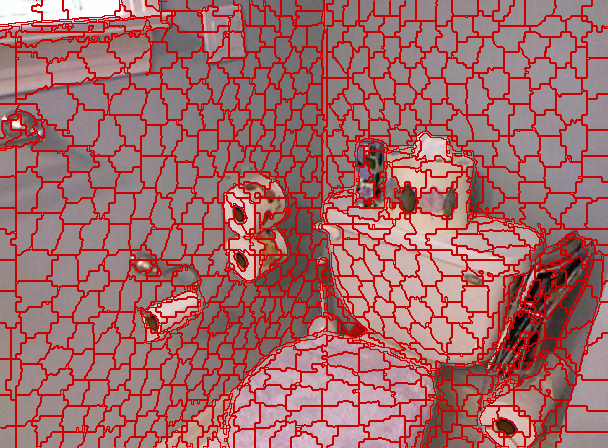
\includegraphics[scale=\scalefivenyu]{pictures/nyu-3-vccs}
	}
	\subfigure{
		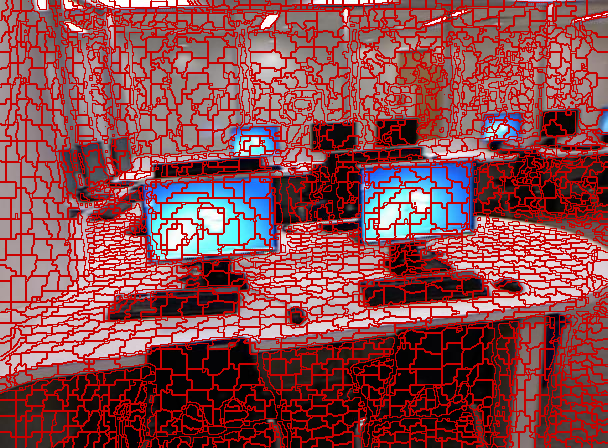
\includegraphics[scale=\scalefivenyu]{pictures/nyu-4-vccs}
	}
	\subfigure{
		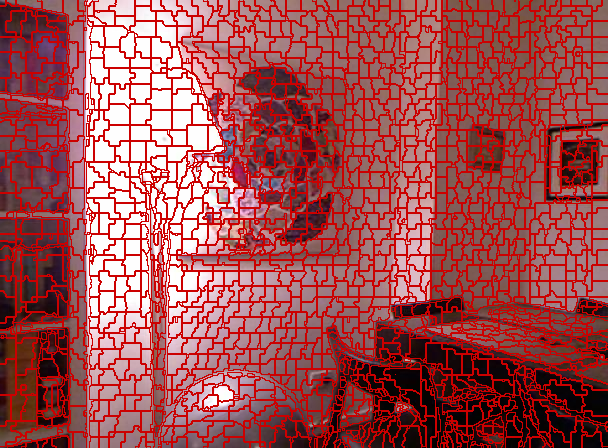
\includegraphics[scale=\scalefivenyu]{pictures/nyu-5-vccs}
	}
%	\subfigure[] {
%		\label{subfig:superpixel-segmentation-vccs-comparison-cloud-1}
%		\includegraphics[scale=0.145]{pictures/nyu-1-vccs-cloud}
%	}
%	\subfigure[] {
%		\label{subfig:superpixel-segmentation-vccs-comparison-cloud-2}
%		\includegraphics[scale=0.155]{pictures/nyu-2-vccs-cloud}
%	}
%	\subfigure[] {
%		\label{subfig:superpixel-segmentation-vccs-comparison-cloud-3}
%		\includegraphics[scale=0.145]{pictures/nyu-3-vccs-cloud}
%	}
	\caption[The running examples oversegmented using \textbf{VCCS} \cite{PaponAbramovSchoelerWoergoetter:2013}.]{The running examples oversegmented into roughly $840$ superpixels using \textbf{VCCS}. Further examples can be found in section \ref{subsection:evaluation-comparison-qualitative} and appendix \ref{chapter:appendix-evaluation}.}
	\label{fig:superpixel-segmentation-depth-vccs-comparison}
\end{figure}
\chapter{SEEDS using Depth Information}
\label{chapter:seeds-depth}

This chapter covers the main topic of this thesis and presents extensions of \textbf{SEEDS} \cite{VanDenBerghBoixRoigCapitaniVanGool:2012} utilizing depth information. In particular, we aim to preserve the framework given by \textbf{SEEDS}, which can best be described as the combination of block and pixel updates, while improving the generated superpixel segmentation. As described in sections \ref{section:seeds-depth-3d-mean-pixel-updates} and \ref{section:seeds-depth-3d-normal-mean-pixel-updates}, integrating depth information into pixel updates can be done similar to \textbf{SLIC3D} and \textbf{DASP} \cite{WeikersdorferGossowBeetz:2012}. However, in our opinion, block updates are responsible for the excellent runtime of \textbf{SEEDS} and therefore we discuss several approaches to improve block updates using depth as well.

% Integrating depth information into \textbf{SEEDS} \cite{VanDenBerghBoixRoigCapitaniVanGool:2012} was the main focus of this thesis. In particular, we wanted to preserve the framework of \textbf{SEEDS}, which can be described as the combination of block and pixel updates, while enhancing the generated superpixel segmentation using depth.
%\begin{algorithm}[b!]
%	\begin{algo}{SEEDS (framework)}{\label{algo:seeds-depth-framework}\qinput{color image $I$, initial block size $w^{(l)} \times h^{(l)}$, histogram size $Q$}\qoutput{superpixel segmentation $S$}}
%		initialization\\
%		\qfor $l = L - 1$ \qto 1\\
%			\qforeach block $B_i^{(l)}$ at level $l$\\
%				perform block update for block $B_i^{(l)}$\qrof\qrof\\
%		\qfor $n = 1$ \qto $N$\\
%			perform pixel update for pixel $x_n$
%	\end{algo}
%	\caption[The basic framework implemented by \textbf{SEEDS} \cite{VanDenBerghBoixRoigCapitaniVanGool:2012}.]{At its heart, \textbf{SEEDS} uses block updates and pixel updates to refine an initial superpixel segmentation.}
%	\label{fig:seeds-depth-framework}
%\end{algorithm}

% As we see in section \ref{section:seeds-depth-3d-mean-pixel-updates} and \ref{section:seeds-depth-3d-normal-mean-pixel-updates}, integrating depth information into pixel updates works similar to \textbf{SLIC3D} and \textbf{DASP} \cite{WeikersdorferGossowBeetz:2012}. Therefore, we focussed on integrating depth information into block updates, because in our opinion, block updates are the main reason for the excellent runtime of \textbf{SEEDS}.

\section{3D Pixel Updates}
\label{section:seeds-depth-3d-mean-pixel-updates}

Similar to \textbf{SLIC3D}, it is possible to integrate 3D point coordinates into mean pixel updates by changing the distance in equation \eqref{eq:superpixel-segmentation-seeds-distance} to
\begin{align}
	\label{eq:seeds-deth-ed-mean-pixels-distance}
	d(x_n, S_j) = \|I(x_n) - I(S_j)\|_2 + \beta\|P(x_n) - P(S_j)\|_2
\end{align}
where $\beta$ can be interpreted as parameter controlling compactness of superpixels within three dimensional space. Using mean pixel updates with the above distance function is referred to as \textbf{SEEDS3D}.
%A suitable normalization is given by
%\begin{align}
%	P =& \left(\max_{x_i} \{P_1(x_i)\} - \min_{x_i} \{P_1(x_i)\}\right)^2 + \left(\max_{x_i} \{P_2(x_i)\} - \min_{x_i} \{P_2(x_i)\}\right)^2\\
%	& + \left(\max_{x_i} \{P_3(x_i)\} - \min_{x_i} \{P_3(x_i)\}\right)^2.
%\end{align}
%Then, algorithm \ref{algo:seeds-depth-3d-mean-pixel-updates} describes the resulting procedure.
%\begin{algorithm}[b!]
%	\begin{algo}{SEEDS (3D mean pixel updates)}{\label{algo:seeds-depth-3d-mean-pixel-updates}\qinput{color image $I$, initial block size $w^{(1)} \times h^{(1)}$, histogram size $Q$}\qoutput{superpixel segmentation $S$}}
%		initialization\\
%		block updates\\
%		\qcom{Initialize superpixel centers}\\
%		\qfor $k = 1$ \qto $K$\\
%			calculate $I(S_k)$ and $P(S_k)$\qrof\\
%		\qfor $n = 1$ \qto $N$\\
%			let $S_j$ be the superpixel $x_n$ belongs to\\
%			\qif a neighboring pixel belongs to a different superpixel $S_k$\\
%				\qthen \qif $d(x_n, S_k) < d(x_n, S_j)$\\
%					\qthen $S_k$ \qlet $S_k \cup \{x_n\}$, $S_j$ \qlet $S_j - \{x_n\}$\qfi\qfi\qrof\\
%		\qreturn $S$
%	\end{algo}
%	\caption{\textbf{SEEDS} extended to use 3D point coordinates for pixel updates.}
%	\label{fig:seeds-depth-3d-mean-pixel-updates}
%\end{algorithm}

\subsection{Discussion}

Although simple, experiments in chapter \ref{chapter:evaluation} show that usage of 3D point coordinates for pixel updates slightly increases performance. This observation can be explained by considering that pixel updates have the greatest influence on the final superpixel segmentation. Therefore, depending on the parameter $\beta$, the above pixel updates are capable of adapting the initial superpixel segmentation to the underlying three dimensional structure. This includes boundaries within the depth image as well as more difficult boundaries between objects in highly cluttered scenes where the above distance prevents superpixels to cover multiple objects and enforces compactness on the object's surface. In contrast to \textbf{VCCS} \cite{PaponAbramovSchoelerWoergoetter:2013}, however, when using a small $\beta$, superpixels may still cover multiple objects even if these objects are not connected in the sense of a voxelized point cloud. Furthermore, the block updates remain unaffected such that the complexity remains unchanged. Figure \ref{fig:seeds-depth-3d-mean-pixels-comparison} shows the running examples oversegmented using \textbf{SEEDS3D}.
\begin{figure}[t]
	\centering
	\subfigure{
		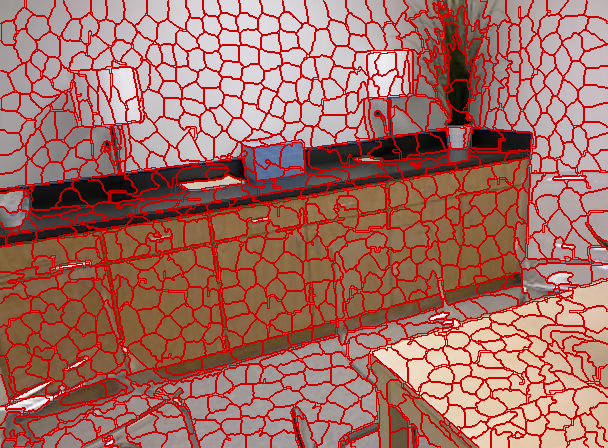
\includegraphics[scale=\scalefivenyu]{pictures/nyu-1-seeds3d}
	}
	\subfigure{
		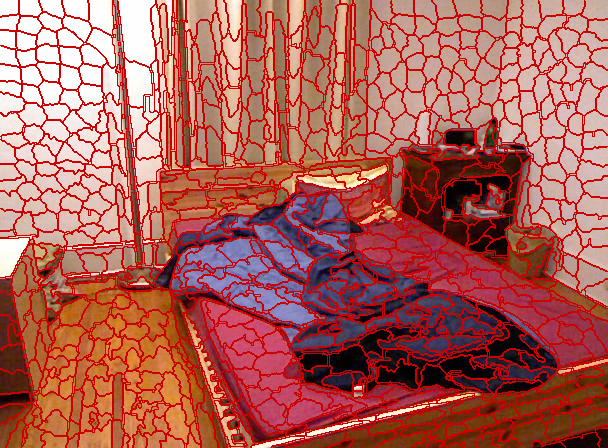
\includegraphics[scale=\scalefivenyu]{pictures/nyu-2-seeds3d}
	}
	\subfigure{
		\includegraphics[scale=\scalefivenyu]{pictures/nyu-3-seeds3d}
	}
	\subfigure{
		\includegraphics[scale=\scalefivenyu]{pictures/nyu-4-seeds3d}
	}
	\subfigure{
		\includegraphics[scale=\scalefivenyu]{pictures/nyu-5-seeds3d}
	}
	\caption[The running examples oversegmented by an extension of \textbf{SEEDS} \cite{VanDenBerghBoixRoigCapitaniVanGool:2012} using 3D point coordinates for pixel updates.]{The running examples oversegmented into exactly $840$ superpixels using \textbf{SEEDS3D}. Further examples are available in section \ref{subsection:evaluation-comparison-qualitative} and appendix \ref{chapter:appendix-evaluation}.}
	\label{fig:seeds-depth-3d-mean-pixels-comparison}
\end{figure}

\section{3D Pixel Updates using Normal Information}
\label{section:seeds-depth-3d-normal-mean-pixel-updates}

Similar to \textbf{DASP}, normal information can be integrated into pixel updates by adapting equation \eqref{eq:seeds-deth-ed-mean-pixels-distance} to
\begin{align}
	\label{eq:seeds-depth-3d-normal-mean-pixels-distance}
	d(x_n, S_j) = \|I(x_n) - I(S_j)\|_2 + \beta\|P(x_n) - P(S_j)\|_2 + \gamma  \arccos \left(N(x_n)^T N(S_j) \right)
\end{align}
where $\beta$ is a compactness parameter and $\gamma$ controls the influence of normal information. Instead of computing the arc-cosine of the dot product $N(x_n)^T N(S_j)$, a distance similar to the one utilized by \textbf{DASP} can be used. This variant of \textbf{SEEDS3D} is in the following referred to as \textbf{SEEDS3Dn}.

The problem of estimating the normal $N(x_n)$ for the point $P(x_n)$ based on a set of points $P(x_{n_1}), \ldots, P(x_{n_k})$ within its local neighborhood is discussed in detail in \cite{Rusu:2009} and several implementations are available as part of the Point Cloud Library \cite{RusuCousins:2011}. For example, using the covariance matric $C$ of the points $P(x_n), P(x_{n_1}), \ldots, P(x_{n_k})$, the normal $N(x_n)$ can be estimated by computing the eigenvalues and eigenvectors of $C$. This corresponds to a first order plane fit. As we can base normal estimation on an ordered point cloud constructed from the depth image $D$, normals can be computed efficiently using integral images, see \cite{HolzerRusuDixonGedikliNavab:2012}. In contrast, \textbf{VCCS} uses least squares plane fits to compute normals within an unordered point cloud and \textbf{DASP} estimates normals purely based on the depth gradient $\nabla D$.

% Computing normals, given a point cloud, can be done using different approaches. In \cite{KlasingAlthoffWollherrBuss:2009} two methods are distinguished: optimization based methods and averaging methods. In general, the problem can be stated as follows: Given a set of points $P(x_1), \ldots, P(x_N)$, we want to estimate a normal $N(x_n)$ for each point using a local neighborhood around the point. For details we refer to \cite{KlasingAlthoffWollherrBuss:2009}. Normals for \textbf{VCCS} are estimated using a least squares plane fit (see the documentation of the Point Cloud Library \cite{Rusu:2009}), while the normals for \textbf{DASP} are based on the depth gradient computed using finite differences. %As discussed in \cite{Rusu:2009}, the normals are not consistently oriented such that they will need to be oriented towards the viewpoint.

\subsection{Discussion}

While normal estimation can be done quite efficiently and results in eligible normal estimates, these are still quite noisy and lack accuracy especially in highly cluttered scenes and at object borders, see figure \ref{fig:seeds-depth-3d-normal-mean-pixels-normal-computation}. Additionally, normals estimated for regions where depth information has been added artificially due to incomplete depth images are not reliable such that normal information should only be used in addition to 3D point coordinates and color.
% Calculating normals using plane fitting can be implemented quite efficiently but lacks accuracy especially at object borders, as demonstrated by figure \ref{fig:seeds-depth-3d-normal-mean-pixels-normal-computation}. Additionally, depth information from RGB-D cameras like the Microsoft Kinect is quite noisy and often contains holes. Therefore, the computed normals may only be used in addition to color and spatial cues in order to improve the generated superpixel segmentation.
\begin{figure}[t]
	\centering
	\subfigure{
		\includegraphics[scale=\scalefivenyu]{pictures/nyu-1-normals-color}
	}
	\subfigure{
		\includegraphics[scale=\scalefivenyu]{pictures/nyu-2-normals-color}
	}
	\subfigure{
		\includegraphics[scale=\scalefivenyu]{pictures/nyu-3-normals-color}
	}
	\subfigure{
		\includegraphics[scale=\scalefivenyu]{pictures/nyu-4-normals-color}
	}
	\subfigure{
		\includegraphics[scale=\scalefivenyu]{pictures/nyu-5-normals-color}
	}
	\subfigure{
		\includegraphics[scale=\scalefivenyu]{pictures/nyu-1-seeds3dn}
	}
	\subfigure{
		\includegraphics[scale=\scalefivenyu]{pictures/nyu-2-seeds3dn}
	}
	\subfigure{
		\includegraphics[scale=\scalefivenyu]{pictures/nyu-3-seeds3dn}
	}
	\subfigure{
		\includegraphics[scale=\scalefivenyu]{pictures/nyu-4-seeds3dn}
	}
	\subfigure{
		\includegraphics[scale=\scalefivenyu]{pictures/nyu-5-seeds3dn}
	}
	\caption[Estimated normals of the running examples color coded and superpixel segmentations generated by an extension of \textbf{SEEDS} \cite{VanDenBerghBoixRoigCapitaniVanGool:2012} using normal information.]{Top: estimated normals for the running examples color coded -- black indicates that no normal could be estimated for this particular pixel. Bottom: the running examples oversegmented into exactly $840$ superpixels using \textbf{SEEDS3Dn}.}
	\label{fig:seeds-depth-3d-normal-mean-pixels-normal-computation}
\end{figure}

As experiments in chapter \ref{chapter:evaluation} show, using normal information for pixel updates results in a negligible performance increase when the normal information is weighted sufficiently low. Whether this is due to the noisy normal computation or the fact that superpixel algorithms using color and 3D point coordinates only already perform well needs to be verified on different datasets. Overall, the running examples oversegmented using \textbf{SEEDS3Dn} are shown in figure \ref{fig:seeds-depth-3d-normal-mean-pixels-normal-computation}.

\section{Mean-Based Block Updates}
\label{section:seeds-depth-mean-block-updates}

Color histograms offer a suitable representation for blocks of pixels. However, as approaches like \textbf{SLIC} \cite{AchantaShajiSmithLucchiFuaSuesstrunk:2010}, \textbf{DASP} and \textbf{VCCS} successfully apply the concept of superpixel centers to superpixel segmentation, it may be beneficial to use similar representations for block updates as well. Consequently, each block $B_i^{(l)}$ is represented by its center and its similarity to a superpixel $S_j$ can be expressed as distance:
\begin{align}
	\label{eq:seeds-depth-mean-block-updates-distance}
	d(B_i^{(l)}, S_j) = \|I(B_i^{(l)}) - I(S_j)\|_2 + \beta\|P(B_i^{(l)}) - P(S_j)\|_2.
\end{align}
The block centers can be pre-computed during initialization, see algorithm \ref{algo:seeds-depth-mean-block-updates}.

The above concept can also be extended to use normal information. In practice, this amounts to computing the blocks mean color and position as well as its orientation. In the simplest form, the orientation $N(B_i^{(l)})$ of block $B_i^{(l)}$ is given by the average of the orientations $N(x_n)$ of the corresponding pixels such that the similarity of block $B_i^{(l)}$ and superpixel $S_j$ can be expressed as
\begin{align}
	d(B_i^{(l)}, S_j) = &\|I(B_i^{(l)}) - I(S_j)\|_2 + \beta\|P(B_i^{(l)}) - P(S_j)\|_2\notag\\
	& + \gamma \arccos \left(N(B_i^{(l)})^T N(S_j) \right).
\end{align}
This is the natural extension of \textbf{SEEDS3Dn} to block updates. Together, the position $P(B_i^{(l)})$ and the orientation $N(B_i^{(l)})$ can be interpreted as plane such that the orientation could also be estimated using a plane fit.
\begin{algorithm}[t]
	\begin{algo}{SEEDS (mean block updates)}{\label{algo:seeds-depth-mean-block-updates}\qinput{color image $I$, block size $w^{(1)} \times h^{(1)}$, number of levels $L$}\qoutput{superpixel segmentation $S$}}
		initialize the block hierarchy and the initial superpixel segmentation $S$\\
		\qcom{Initialization of block/superpixel centers:}\\
		\qfor $l = 1$ \qto $L$\\
			\qforeach block $B_i^{(l)}$ at level $l$ \qcom{For $l = L$ these are the initial superpixels.}\\ 
				compute $I(B_i^{(l)})$ and $P(B_i^{(l)})$\qrof\qrof\\
		\qcom{Mean based block updates:}\\
		\qfor $l = L - 1$ \qto $1$\\
			\qforeach block $B_i^{(l)}$ at level $l$\\
				let $S_j$ be the superpixel $B_i^{(l)}$ belongs to\\
				\qif a neighboring block belongs to a different superpixel $S_k$\\
					\qthen \qif $d(B_i^{(l)}, S_k) < d(B_i^{(l)}, S_j)$\\
						\qthen $S_k$ \qlet $S_k \cup B_i^{(l)}$ and $S_j$ \qlet $S_j - B_i^{(l)}$\qfi\qfi\qrof\qrof\\
		%\qcom{Note that for mean pixel updates, the superpixel centers are already computed.}\\
		mean pixel updates \qcom{Note that the superpixel centers are already available.}\\
		\qreturn S
	\end{algo}
	\caption[\textbf{SEEDS} \cite{VanDenBerghBoixRoigCapitaniVanGool:2012} based on mean block updates using 3D point coordinates.]{After defining a distance $d(B_i^{(l)}, S_j)$ between blocks and superpixels based on their respective centers, block updates can be performed without relying on color histograms. Of course, both approaches can also be combined resulting in a higher runtime}
	\label{fig:seeds-depth-mean-block-updates}
\end{algorithm}

\subsection{Discussion}

Unfortunately, block centers appear to be a poor representation for blocks of pixels. For example consider the running examples in figure \ref{fig:seeds-depth-mean-block-updates-discussion-blocks}. Choosing a block crossing a strong boundary between different objects, a color histogram is able to capture both parts of the block by having two modes. However, the block center may capture information not present within the block. In contrast, superpixels computed after performing block updates at level $l = 1$ appear to be homogeneous in color and cover mostly one object such that using superpixel centers is appropriate for pixel updates. Therefore, using mean position and color as representation of superpixels is appropriate only when given a sound initial superpixel segmentation and consequently blocks of pixels are better represented by color histograms.
\begin{figure}[t]
	\centering
	\subfigure{
		\includegraphics[scale=\scalefivenyu]{pictures/nyu-1-seeds-level-4}
	}
	\subfigure{
		\includegraphics[scale=\scalefivenyu]{pictures/nyu-2-seeds-level-4}
	}
	\subfigure{
		\includegraphics[scale=\scalefivenyu]{pictures/nyu-3-seeds-level-4}
	}
	\subfigure{
		\includegraphics[scale=\scalefivenyu]{pictures/nyu-4-seeds-level-4}
	}
	\subfigure{
		\includegraphics[scale=\scalefivenyu]{pictures/nyu-5-seeds-level-4}
	}
	\subfigure{
		\includegraphics[scale=\scalefivenyu]{pictures/nyu-1-seeds-after-1}
	}
	\subfigure{
		\includegraphics[scale=\scalefivenyu]{pictures/nyu-2-seeds-after-1}
	}
	\subfigure{
		\includegraphics[scale=\scalefivenyu]{pictures/nyu-3-seeds-after-1}
	}
	\subfigure{
		\includegraphics[scale=\scalefivenyu]{pictures/nyu-4-seeds-after-1}
	}
	\subfigure{
		\includegraphics[scale=\scalefivenyu]{pictures/nyu-5-seeds-after-1}
	}
	\caption[An illustration of the disadvantages of using block centers to perform block updates.]{Top: Block segmentations at level $(L - 1)$. Bottom: superpixel segmentations before performing pixel updates.}
	\label{fig:seeds-depth-mean-block-updates-discussion-blocks}
\end{figure}
The same considerations apply for averaging normals. Therefore, we used the covariance matrix to estimate the orientation of the blocks and superpixels. However, after each update, the orientation of the corresponding superpixels need to be recomputed. Although this approach is comparably inefficient, our experiments show that even after computing the optimal orientation in the least squares sense, using normal information does not increase performance.
Furthermore, computing block centers at lower levels, where each block contains only few pixels, is highly influenced by outliers and noise. Overall, these considerations imply that mean based block updates perform poorly when compared to the original block updates in algorithm \ref{algo:superpixel-segmentation-seeds}. This can also be interpreted as motivation of superpixel growing as done by \textbf{SLIC}, \textbf{DASP} and \textbf{VCCS}.

% TODO: Introduce "3D mean pixels".
%The above discussion can be supported by experiments. Figure \ref{fig:seeds-depth-mean-block-updates-discussion-comparison} compares several images when segmented using usual block updates and 3D mean pixel updates and mean based block updates.
%\begin{figure}
%	% TODO: runnign examples compared (have to reimplement mean based updates).
%	\label{fig:seeds-depth-mean-block-updates-discussion-comparison}
%\end{figure}

\section{Block Updates Based on Normal Histograms}
\label{section:deeds-depth-normal-histograms}

As color histograms appear to work well as representations for blocks of pixels, it appears to be advantageous to integrate depth information in the form of histograms. Depth histograms, however, do not offer an increase in performance. Therefore, we would like block updates to capture normal information instead. This can be accomplished using histograms of normal orientation which we refer to as normal histograms.

Given a point normal $N(x_n)$ with components $N_1(x_n), N_2(x_n), N_3(x_n)$, the orientation can be split up into the polar angle $\phi$ between normal and the y-axis, and the azimuthal angle $\theta$ between normal and x-axis, see figure \ref{fig:seeds-depth-normal-histograms-angles}.
The angles are binned to form a two dimensional histogram and the similarity of a block and a superpixel is then expressed as the intersection of these histograms. This can be weighted and used in combination with color histograms.
% taken from: http://www.texample.net/tikz/examples/the-3dplot-package/
\begin{SCfigure}[2\sidecaptionrelwidth][b]
	%set the plot display orientation
	%synatax: \tdplotsetdisplay{\theta_d}{\phi_d}
	\tdplotsetmaincoords{60}{110}

	%define polar coordinates for some vector
	%TODO: look into using 3d spherical coordinate system
	\pgfmathsetmacro{\rvec}{.4}
	\pgfmathsetmacro{\thetavec}{30}
	\pgfmathsetmacro{\phivec}{60}
	\begin{tikzpicture}[scale=5,tdplot_main_coords]

		%set up some coordinates 
		%-----------------------
		\coordinate (O) at (0,0,0);
		
		%determine a coordinate (P) using (r,\theta,\phi) coordinates.  This command
		%also determines (Pxy), (Pxz), and (Pyz): the xy-, xz-, and yz-projections
		%of the point (P).
		%syntax: \tdplotsetcoord{Coordinate name without parentheses}{r}{\theta}{\phi}
		\tdplotsetcoord{P}{\rvec}{\thetavec}{\phivec}
		\tdplotsetcoord{N}{\rvec + 0.2}{\thetavec}{\phivec}

		%draw figure contents
		%--------------------

		%draw the main coordinate system axes
		\draw[thick,->] (0,0,0) -- (0.5,0,0) node[anchor=north east]{$x$};
		\draw[thick,->] (0,0,0) -- (0,0.5,0) node[anchor=north west]{$z$};
		\draw[thick,->] (0,0,0) -- (0,0,0.5) node[anchor=south]{$y$};
		
		%draw a vector from origin to point (P) 
		\draw[-stealth,color=red] (O) -- (P);
		\node at (N) {$N(x_n)$};

		%draw projection on xy plane, and a connecting line
		\draw[dashed, color=red] (O) -- (Pxy);
		\draw[dashed, color=red] (P) -- (Pxy);

		%draw the angle \phi, and label it
		%syntax: \tdplotdrawarc[coordinate frame, draw options]{center point}{r}{angle}{label options}{label}
		\tdplotdrawarc{(O)}{0.15}{0}{\phivec}{anchor=north}{$\theta$}

		%set the rotated coordinate system so the x'-y' plane lies within the
		%"theta plane" of the main coordinate system
		%syntax: \tdplotsetthetaplanecoords{\phi}
		\tdplotsetthetaplanecoords{\phivec}

		%draw theta arc and label, using rotated coordinate system
		\tdplotdrawarc[tdplot_rotated_coords]{(0,0,0)}{0.25}{0}{\thetavec}{anchor=south}{$\phi$}

		%draw some dashed arcs, demonstrating direct arc drawing
		\draw[dashed,tdplot_rotated_coords] (\rvec,0,0) arc (0:90:\rvec);
		\draw[dashed] (\rvec,0,0) arc (0:90:\rvec);

		%set the rotated coordinate definition within display using a translation
		%coordinate and Euler angles in the "z(\alpha)y(\beta)z(\gamma)" euler rotation convention
		%syntax: \tdplotsetrotatedcoords{\alpha}{\beta}{\gamma}
		\tdplotsetrotatedcoords{\phivec}{\thetavec}{0}

		%translate the rotated coordinate system
		%syntax: \tdplotsetrotatedcoordsorigin{point}
		\tdplotsetrotatedcoordsorigin{(P)}

		%change the rotated coordinate frame so that it lies in its theta plane.
		%Note that this overwrites the original rotated coordinate frame
		%syntax: \tdplotsetrotatedthetaplanecoords{\phi'}
		\tdplotsetrotatedthetaplanecoords{45}

	\end{tikzpicture}
	\caption[Illustration of the binning of normal orientation into histograms.]{Point normals are binned using the polar angle $\phi$ between normal and $y$-axis and the azimuthal angle $\theta$ between normal and $x$-axis. In practice, the normal is always oriented towards the viewpoint such that $\phi, \theta \in [0,180^\circ]$.}
	\label{fig:seeds-depth-normal-histograms-angles}
\end{SCfigure}

\subsection{Discussion}
\label{subsection:deeds-depth-normal-histograms-discussion}

Considering the binning of the normals, we came to the conclusion that an odd number of bins per angle should be used. This is based on the following case: We consider a normal with $\phi = 90^\circ$ and $\theta = 90^\circ$. As this normal is not estimated perfectly, the angles would lie slightly below or above the $90^\circ$ such that the actual bin depends on the noise and the estimation method which should be avoided to get an adequate representation of surfaces parallel to the image plane.
%This is illustrated in figure \ref{fig:seeds-depth-normal-histograms-binning}.
%\begin{figure}
%	% TODO: figure for binning.
%	\label{fig:seeds-depth-normal-histograms-binning}
%\end{figure}

Overall, experiments show that this extension does not improve performance while additionally increasing runtime. In our opinion, the main reasons for this observation are the following. Firstly, as stated in section \ref{section:seeds-depth-3d-normal-mean-pixel-updates}, a superpixel segmentation obtained by running \textbf{SEEDS} based purely on color achieves state-of-the-art performance leaving only little room for improvement. Secondly, the most difficult regions within images taken from the NYU Depth Dataset \cite{SilbermanHoiemKohliFergus:2012} contain plenty of small objects -- often the scenes are highly cluttered. In such settings, the estimated normals tend to be highly unrepresentative and noisy. In contrast, in regions of nearly planar surfaces, where we expect normal information to be of help, oversegmentations based on color only usually yield high performance. In conclusion, we find that normal histograms are not worth their computation time. Figure \ref{fig:seeds-depth-normal-histograms-comparison} shows the running examples oversegmented using normal histograms. As pixel updates have not been adapted, the results differ only slightly from those presented in figure \ref{fig:seeds-depth-3d-mean-pixels-comparison}. In contrast, when using pixel updates based on color and normal histograms similar to those in algorithm \ref{algo:superpixel-segmentation-seeds}, the superpixel segmentations appear to have low quality.
\begin{figure}[t]
	\centering
	\subfigure{
		\includegraphics[scale=\scalefivenyu]{pictures/nyu-1-seeds-normal-histograms}
	}
	\subfigure{
		\includegraphics[scale=\scalefivenyu]{pictures/nyu-2-seeds-normal-histograms}
	}
	\subfigure{
		\includegraphics[scale=\scalefivenyu]{pictures/nyu-3-seeds-normal-histograms}
	}
	\subfigure{
		\includegraphics[scale=\scalefivenyu]{pictures/nyu-4-seeds-normal-histograms}
	}
	\subfigure{
		\includegraphics[scale=\scalefivenyu]{pictures/nyu-5-seeds-normal-histograms}
	}
	\subfigure{
		\includegraphics[scale=\scalefivenyu]{pictures/nyu-1-seeds-normal-histograms-pixel}
	}
	\subfigure{
		\includegraphics[scale=\scalefivenyu]{pictures/nyu-2-seeds-normal-histograms-pixel}
	}
	\subfigure{
		\includegraphics[scale=\scalefivenyu]{pictures/nyu-3-seeds-normal-histograms-pixel}
	}
	\subfigure{
		\includegraphics[scale=\scalefivenyu]{pictures/nyu-4-seeds-normal-histograms-pixel}
	}
	\subfigure{
		\includegraphics[scale=\scalefivenyu]{pictures/nyu-5-seeds-normal-histograms-pixel}
	}
	\caption[Superpixel segmentations of the running examples generated by a variant of \textbf{SEEDS} \cite{VanDenBerghBoixRoigCapitaniVanGool:2012} based on normal histograms.]{Top: the running examples oversegmented using normal histograms for block updates. Bottom: superpixel segmentations with exactly $840$ superpixels of the running examples generated using normal histograms for both block updates and pixel updates.}
	\label{fig:seeds-depth-normal-histograms-comparison}
\end{figure}

%\section{Block Updates Based on Plane Fitting}
%
%Combining both normal information as well as the concept of block centers, an interesting representation of a block of pixels is given by a plane fit for the corresponding 3D point coordinates. Similar to normal estimation, this can be done using the covariance matrix of all points $P(x_n)$ within the block. However, the covariance matrix of each superpixel has to be recomputed after each block or pixel update based on the superpixel's center. An alternative is given by averaging methods as for example described by Klasing \etal \cite{KlasingAlthoffWollherrBuss:2009}. Using averaging methods, planes could be estimated incrementally such that block and pixel updates can be performed more efficiently. In its simplest form this would mean to average the point normals $N(x_n)$ for all points within the block. Overall, given a block $B_i^{(l)}$ and a superpixel $S_j$, we can compute the angle between the corresponding normals to get a further clue of their similarity:
%\begin{align}
%	\arccos\left(N(B_i^{(l)})^T N(S_j)\right).
%\end{align}
%This can 
%
%In the following, we review the above considerations in detail.\\
%Plane Fitting: Given a block $B_i^{(l)}$ with pixels $x_{n_1},\ldots,x_{n_k}$, we aim to fit a plane characterized by
%\begin{align}
%	\label{eq:seeds-depth-plane}
%	N_1(B_i^{(l)}) P_1(x_{n_j}) + N_3(B_i^{(l)}) P_3(x_{n_j}) + N_3(B_i^{(l)}) P_3(x_{n_j}) + d = 0\quad \forall 1 \leq j \leq k.
%\end{align}
%This leads to solving
%\begin{align}
%	\left\| \begin{pmatrix} \boldsymbol P &\boldsymbol 1 \end{pmatrix} \begin{pmatrix} N_1(B_i^{(l)})\\ N_2(B_i^{(l)})\\ N_3(B_i^{(l)}) \end{pmatrix} \right\|_2 \rightarrow \min
%\end{align}
%where $\boldsymbol P$ is the matrix containing the points $P(x_{n_1}), \ldots, P(x_{n_k})$ in its rows and $\boldsymbol 1~=~(1, \ldots, 1)^T$. This can be solved utilizing Singular Value Decomposition (\eg see \cite{ForsythPonce:2002}).\\
%%As alternative, the mean can be computed as usual and the normal can be estimated using an averaging method. Let $T(B_i^{(l)})$ be the set of all subsets of size three of $B_i^{(l)}$. Then the normal can be estimated as
%%\begin{align}
%%	N(B_i^{(l)}) = \frac{1}{|T(B_i^{(l)})|} \sum_{\{x_i,x_j,x_k\} \in T(b_i^{(l)})  \frac{(x_j - x_i) \times (x_k - x_i)}{\|(x_j - x_i) \times (x_k - x_i)\|_2}
%%\end{align}
%%where $\times$ denotes the cross product. The uniform weighting factor can also be replaced by their weighting schemes \cite{KlasingAlthoffWollherrBuss:2009}. Such an estimate can be updated easily after exchanging blocks or pixels.
%% TODO: check correct angle comptuation for DASP, VCCS, 3D (Normal) Mean Pixels
%Block Updates: Given block $B_i^{(l)}$ and superpixel $S_j$, the similarity of block $B_i^{(l)}$ to superpixel $S_j$ can be expressed as
%\begin{align}
%	d(B_i^{(l)}, S_j) = \frac{N(B_i^{(l)})^T N(S_j)}{\|N(B_i^{(l)})\|_2 \|N(S_j)\|_2}.
%\end{align}
%This can then be combined with color histograms and is similar to using mean block updates where additionally normal information is used to characterize the block and superpixel centers.\\
%Pixel Updates: The distance of a point $P(x_n)$ to the plane of superpixel $S_j$ can be calculated as
%\begin{align}
%	d(x_n, S_j) = \frac{(P(x_n) - P(S_j))^T N(S_j)}{\|N(S_j)\|_2}.
%\end{align}
%However, the euclidean distance to the superpixel center appears to be more appropriate and reliable as the above equation performs an orthogonal projection. Again, this has to be combined with a color term which is either based on color histograms or the euclidean distance in color space.\\
%Overall, the above considerations are similar to the idea of performing mean based block updates. When using averaging methods to estimate the plane of equation \eqref{eq:seeds-depth-plane} this approach actually boils down to use mean based block updates with normal information. However, estimating the planes based on sufficient statistics which could be updated incremental is possible as well.
%
%\subsection{Discussion}
%
%As discussed in sections \ref{section:seeds-depth-mean-block-updates} and \ref{section:seeds-depth-3d-normal-mean-pixel-updates}, the main problem with this approach is the initial superpixel segmentation. The fitted planes are initially highly unrepresentative. For small blocks, noisy pixels and outliers worsen the estimated planes. Furthermore, the most interesting and difficult objects within the scenes cannot be represented by a set of planes (see discussion in section \ref{subsection:deeds-depth-normal-histograms-discussion}). Overall, as we expected after experimenting with normal histograms, planes are not an appropriate representation and strongly increase runtime as well as performance.
\chapter{Datasets and Benchmarks}
\label{chapter:datasets}

In this chapter we discuss two popular datasets for evaluating segmentation algorithms: the Berkeley Segmentation Dataset \cite{ArbelaezMaireFowlkesMalik:2011} and the NYU Depth Dataset \cite{SilbermanHoiemKohliFergus:2012}. Furthermore, we discuss several measures used to assess superpixel algorithms which have, in the course of this thesis, been implemented as extension of the Berkeley Segmentation Benchmark which is provided as part of the Berkeley Segmentation Dataset by Arbel\'aez \etal \cite{ArbelaezMaireFowlkesMalik:2011}.

\section{Berkeley Segmentation Dataset}

\begin{figure}[b]
	\subfigure{
		\includegraphics[scale=\scalefivebsd]{pictures/bsd-3-ground-truth-1}
	}
	\subfigure{
		\includegraphics[scale=\scalefivebsd]{pictures/bsd-3-ground-truth-2}
	}
	\subfigure{
		\includegraphics[scale=\scalefivebsd]{pictures/bsd-3-ground-truth-3}
	}
	\subfigure{
		\includegraphics[scale=\scalefivebsd]{pictures/bsd-3-ground-truth-4}
	}
	\subfigure{
		\includegraphics[scale=\scalefivebsd]{pictures/bsd-3-ground-truth-5}
	}
	\subfigure{
		\includegraphics[scale=0.1535]{pictures/bsd-3-ground-truth-1-lines}
	}
	\subfigure{
		\includegraphics[scale=0.1535]{pictures/bsd-3-ground-truth-2-lines}
	}
	\subfigure{
		\includegraphics[scale=0.1535]{pictures/bsd-3-ground-truth-3-lines}
	}
	\subfigure{
		\includegraphics[scale=0.1535]{pictures/bsd-3-ground-truth-4-lines}
	}
	\subfigure{
		\includegraphics[scale=0.1535]{pictures/bsd-3-ground-truth-5-lines}
	}
	\caption[Several ground truth segmentations of one of the running examples as provided by the Berkeley Segmentation Dataset \cite{ArbelaezMaireFowlkesMalik:2011}.]{Ground truth segmentations of one of the running examples as provided by the BSDS500.}
	\label{fig:datasets-bsd-ground-truth}
\end{figure}
The first version of the Berkeley Segmentation Dataset, introduced in \cite{MartinFowlkesTalMalik:2001} and referred to as BSDS300, comprises $300$ images split up into a training set of $200$ images and a test set of $100$ images. The second version \cite{ArbelaezMaireFowlkesMalik:2011}, referred to as BSDS500, adds $200$ additional images forming a new test set while the old test set is used as validation set instead. Per image, at least five ground truth segmentations are available, each annotated by a different person, see for example figure \ref{fig:datasets-bsd-ground-truth}. Therefore, the ground truth segmentations are highly varying and reflect the difficult nature of segmenting natural images. Overall, this results in a fair evaluation of superpixel algorithms as for each superpixel segmentation a suitable ground truth segmentation can be chosen or the average performance over the ground truth segmentations can be computed. In practice, concerning all measures based on ground truth segmentations presented in this chapter, for each image we choose the ground truth segmentation resulting in the best value and subsequently average over all images. However, note that some of the measures provided as part of the Berkeley Segmentation Benchmark offer natural extensions to multiple ground truth segmentations, as for example the Probabilistic Rand Index \cite{UnnikrishnanPantofaruHebert:2007}, see appendix \ref{chapter:appendix-berkeley-segmentation-benchmark}.
% The first version, referred to as BSDS300, comprises $300$ images and was introduced in \cite{MartinFowlkesTalMalik:2001}. The dataset is split into a training set of $200$ images and a test set of $100$ images. For each image there are five ground truth segmentations available. The second version, introduced in \cite{ArbelaezMaireFowlkesMalik:2011}, adds $200$ additional images and is referred to as BSDS500. The old test set forms a validation set and the new $200$ images form the new test set. We use the BSDS500 as it is provided (no pre-processing is necessary). The images have size $321 \times 481$ or $481 \times 321$ depending on the aspect ratio. Figures \ref{subfig:introduction-running-examples-bsd-1} - \ref{subfig:introduction-running-examples-bsd-3} are taken from the validation set of the BSDS500.
%Figure \ref{fig:datasets-berkeley-segmentation-dataset-ground-truth} shows two of the provided ground truth segmentation, respectively.
%\begin{figure}
%	\subfigure[]{
%		\label{subfig:datasets-berkeley-segmentation-dataset-ground-truth-1-1}
%		\includegraphics[scale=\scalethreebsd]{pictures/bsd-1-ground-truth-1}
%	}
%	\subfigure[]{
%		\label{subfig:datasets-berkeley-segmentation-dataset-ground-truth-2-1}
%		\includegraphics[scale=\scalethreebsd]{pictures/bsd-2-ground-truth-1}
%	}
%	\subfigure[]{
%		\label{subfig:datasets-berkeley-segmentation-dataset-ground-truth-3-1}
%		\includegraphics[scale=\scalethreebsd]{pictures/bsd-3-ground-truth-1}
%	}
%	\subfigure[]{
%		\label{subfig:datasets-berkeley-segmentation-dataset-ground-truth-1-2}
%		\includegraphics[scale=\scalethreebsd]{pictures/bsd-1-ground-truth-2}
%	}
%	\subfigure[]{
%		\label{subfig:datasets-berkeley-segmentation-dataset-ground-truth-2-2}
%		\includegraphics[scale=\scalethreebsd]{pictures/bsd-2-ground-truth-2}
%	}
%	\subfigure[]{
%		\label{subfig:datasets-berkeley-segmentation-dataset-ground-truth-3-2}
%		\includegraphics[scale=\scalethreebsd]{pictures/bsd-3-ground-truth-2}
%	}
%	\caption[Ground truth segmentations for the running examples as provided by the Berkeley Segmentation Dataset \cite{ArbelaezMaireFowlkesMalik:2011}.]{A selection of two ground truth segmentations of the running examples shown in figures \ref{subfig:introduction-running-examples-bsd-1} - \ref{subfig:introduction-running-examples-bsd-3}, respectively.}
%	\label{fig:datasets-berkeley-segmentation-dataset-ground-truth}
%\end{figure}

\begin{figure}[t]
	\centering
	\subfigure{
		\includegraphics[scale=\scalefivenyu]{pictures/nyu-1-labels}
	}
	\subfigure{
		\includegraphics[scale=\scalefivenyu]{pictures/nyu-2-labels}
	}
	\subfigure{
		\includegraphics[scale=\scalefivenyu]{pictures/nyu-3-labels}
	}
	\subfigure{
		\includegraphics[scale=\scalefivenyu]{pictures/nyu-4-labels}
	}
	\subfigure{
		\includegraphics[scale=\scalefivenyu]{pictures/nyu-5-labels}
	}
	\subfigure{
		\includegraphics[scale=0.16]{pictures/nyu-1-labels-thinned}
	}
	\subfigure{
		\includegraphics[scale=0.16]{pictures/nyu-2-labels-thinned}
	}
	\subfigure{
		\includegraphics[scale=0.16]{pictures/nyu-3-labels-thinned}
	}
	\subfigure{
		\includegraphics[scale=0.16]{pictures/nyu-4-labels-thinned}
	}
	\subfigure{
		\includegraphics[scale=0.16]{pictures/nyu-5-labels-thinned}
	}
	\caption[Structure labels of the running examples as provided by the NYU Depth Dataset \cite{SilbermanHoiemKohliFergus:2012} and after removing small unlabeled regions in between larger labeled regions.]{The NYUV2 provides a high variety of different labels. In \cite{SilbermanHoiemKohliFergus:2012}, Silberman \etal grouped these labels to obtain a total of four so called structure labels. Top: the structure labels as provided by the NYUV2. Bottom: the structure labels after removing thin unlabeled regions in between larger labeled regions. Black indicates unlabeled pixels. Overall, this illustrates why the dataset is considered harder in comparison to the natural images from the BSDS500.}
	\label{fig:datasets-nyu-depth-dataset-labels}
\end{figure}
\section{NYU Depth Dataset}

The first version of the NYU Depth Dataset, in the following referred to as NYUV1, was introduced in \cite{SilbermanFergus:2011} by Silberman \etal. The dataset comprises $2284$\footnote{Although, Silberman \etal mention $2347$ labeled frames \cite{SilbermanFergus:2011}, we found that, actually, the dataset comprises only $2284$ labeled frames.} labeled frames taken from video sequences showing six different indoor scenes. The video sequences were taken by a calibrated Microsoft Kinect \cite{SilbermanFergus:2011} such that depth information is accessible. The frames were annotated using the LabelMe tool \cite{RussellTorralbaMurphyFreeman:2008} resulting in around $1000$ classes which are highly redundant \cite{SilbermanFergus:2011}.

The second version of the NYU Depth Dataset \cite{SilbermanHoiemKohliFergus:2012}, NYUV2, adds further variety in the form of indoor scenes from different cities as well as commercial accommodations. The dataset comprises $1449$ labeled frames with a total of $894$ classes \cite{SilbermanHoiemKohliFergus:2012}. Every instance of a particular class within a single frame gets a unique instance label. Following Ren and Bo \cite{RenBo:2012} we combine class labels and instance labels to generate ground truth segmentations compatible with the Berkeley Segmentation Benchmark. Although Silberman \etal state that the annotators were instructed to provide a dense labeling of the scenes, the images often contain small unlabeled regions in between larger labeled regions, see figure~\ref{fig:datasets-nyu-depth-dataset-labels}. Therefore, based on code provided by Ren and Bo \cite{RenBo:2012}, we remove these small background regions. Furthermore, bad lighting as well as cluttered scenes account for the difficulty of the NYUV2. However, this also represents an appropriate contrast to the natural images of the BSDS500.
% Therefore, based on the measures introduced in section \ref{section:datasets-extended-berkeley-segmentation-benchmark}, the dataset is overall harder to oversegment. However, this may also be due to the chosen scenes. In contrast to the BSDS500, the NYU Depth Dataset contains indoor scenes which are mostly untidy and highly cluttered. Additionally, only one ground truth segmentation per frame is provided. 

\begin{figure}[t]
	\centering
	\subfigure{
		\includegraphics[scale=\scalefiveoriginalnyu]{pictures/nyu-1-raw-depth}
	}
	\subfigure{
		\includegraphics[scale=\scalefiveoriginalnyu]{pictures/nyu-2-raw-depth}
	}
	\subfigure{
		\includegraphics[scale=\scalefiveoriginalnyu]{pictures/nyu-3-raw-depth}
	}
	\subfigure{
		\includegraphics[scale=\scalefiveoriginalnyu]{pictures/nyu-4-raw-depth}
	}
	\subfigure{
		\includegraphics[scale=\scalefiveoriginalnyu]{pictures/nyu-5-raw-depth}
	}
	\subfigure{
		\includegraphics[scale=\scalefiveoriginalnyu]{pictures/nyu-1-depth}
	}
	\subfigure{
		\includegraphics[scale=\scalefiveoriginalnyu]{pictures/nyu-2-depth}
	}
	\subfigure{
		\includegraphics[scale=\scalefiveoriginalnyu]{pictures/nyu-3-depth}
	}
	\subfigure{
		\includegraphics[scale=\scalefiveoriginalnyu]{pictures/nyu-4-depth}
	}
	\subfigure{
		\includegraphics[scale=\scalefiveoriginalnyu]{pictures/nyu-5-depth}
	}
	\caption[The raw depth mages as well as the pre-processed depth images from the running examples as provided by the NYU Depth Dataset \cite{SilbermanHoiemKohliFergus:2012}.]{Top: the raw depth images corresponding to the running examples where black regions indicate that no depth information is available. Bottom: the pre-processed depth images corresponding to the running examples.}
	\label{fig:datasets-nyu-depth-dataset-depth}
\end{figure}

The NYUV2 includes both the raw depth images as well as a pre-processed version. The provided raw depth images have been aligned with the corresponding color images, however, the region covered by the depth images is significantly smaller and reflective surfaces such as mirrors and windows cause holes within the depth images. Therefore, Silberman \etal provide a pre-processed version of the depth images where these regions have been filled artificially. This is illustrated in figure \ref{fig:datasets-nyu-depth-dataset-depth}, showing both the raw depth images as well as the pre-processed depth images of the running examples. Furthermore, the provided images have been undistorted resulting in a small white border around the actual images. Therefore, we crop the images of size $640 \times 480$ to obtain images of size $608 \times 448$ without white borders. Finally, we choose $200$ images to form a training set and $400$ images to form a test set both including most of the available indoor scenes\footnote{Our split is based on a training/test split provided by Ren and Bo \cite{RenBo:2012}. However, to speed up evaluation, we reduced the size of the sets to $200$ and $400$, respectively. The images have been chosen such that almost all scenes are represented.}.

\section{Extended Berkeley Segmentation Benchmark}
\label{section:datasets-extended-berkeley-segmentation-benchmark}

Most measures provided as part of the Berkeley Segmentation Benchmark are unsuited for evaluating superpixel algorithms, see appendix \ref{chapter:appendix-berkeley-segmentation-benchmark}. Therefore, in this section, we discuss most of the available measures used to evaluate superpixel algorithms. These have, except for Boundary Recall, in the course of this thesis, been implemented into the framework of the Berkeley Segmentation Benchmark.

\subsection{Boundary Recall}

Boundary Recall is part of the Precision-Recall-Framework introduced in \cite{MartinFowlkesMalik:2004} which is discussed in detail in appendix \ref{chapter:appendix-berkeley-segmentation-benchmark}. Let $S$ be a superpixel segmentation and $G$ be a ground truth segmentation, then we define:
\begin{description}
 	\item[True Positives, $TP(S, G)$:] Boundary pixels in $G$ for which there is a boundary pixel in $S$ in range~$r$.
	\item[False Negatives, $FN(S, G)$:] Boundary pixels in $G$ for which there is no boundary pixel in $S$ in range~$r$.
\end{description}
where $r$ defines a tolerance parameter controlling the allowed deviation from the ground truth. In practice, $r$ is set to $0.0075$ times the image diagonal\footnote{This is the default value as used by the Berkeley Segmentation Benchmark and we chose not to change this value to keep our results comparable to other publications.}.
The Boundary Recall $Rec(S,G)$ is the fraction of all boundary pixels within the ground truth segmentation $G$ which are correctly detected within the superpixel segmentation $S$, that is
\begin{align}
	Rec(S,G) = \frac{|TP(S,G)|}{|TP(S,G)| + |FN(S,G)|}.
\end{align}
As we want superpixels to respect the boundaries within the image, a high Boundary Recall is desirable.

\subsection{Undersegmentation Error}
\label{subsection:datasets-extended-berkeley-segmentation-benchmark-undersegmentation-error}

The Undersegmentation Error describes the leakage or ``bleeding'' \cite{LevinshteinStereKutulakosFleetDickinsonSiddiqi:2009} of a superpixel with respect to a specific ground truth segment. In \cite{LiuTuzelRamalingamChellappa:2011} and \cite{VekslerBoykovMehrani:2010}, the Undersegmentation Error is defined as
\begin{align}
	\label{eq:datasets-extended-berkeley-segmentation-benchmark-ue-old}
	UE(S,G) = \frac{1}{N} \left( \sum_{G_i \in G} \left( \sum_{S_j \cap G_i \neq \emptyset} |S_j|\right) - N\right).
\end{align}
This equation computes the total amount of leakage for all ground truth segments and normalizes the sum by the number of pixels\footnote{We note that equation \eqref{eq:datasets-extended-berkeley-segmentation-benchmark-ue-old} uses a slightly different normalization when compared to the Undersegmentation Error as used by Levinshtein \etal in \cite{LevinshteinStereKutulakosFleetDickinsonSiddiqi:2009}.}. We note that the normalization used above may not be sufficient. For example consider a superpixel segmentation with a single superpixel covering the whole image. Then, if the ground truth consists of more than two segments, the Undersegmentation Error will be greater than one. In addition, as stated by Neubert and Protzel \cite{NeubertProtzel:2012} as well as Achanta \etal \cite{AchantaShajiSmithLucchiFuaSuesstrunk:2010} this definition has another serious disadvantage. Consider a large superpixel covering one ground truth segment perfectly except for some pixels. In the above equation, such superpixels receive high penalties \cite{NeubertProtzel:2012}. Achanta \etal adapt equation \eqref{eq:datasets-extended-berkeley-segmentation-benchmark-ue-old} to tolerate a small amount of leakage per superpixel:
\begin{align}
	UE(S,G) = \frac{1}{N} \left( \sum_{G_i \in G} \left( \sum_{|S_j \cap G_i| > B} |S_j|\right) - N\right)
\end{align}
where $B$ is the corresponding tolerance parameter. To avoid an additional parameter, we implemented the Undersegmentation Error as proposed by Neubert and Protzel:
\begin{align}
	\label{eq:datasets-extended-berkeley-segmentation-benchmark-ue}
	UE(S,G) = \frac{1}{N} \sum_{G_i \in G} \sum_{S_j \cap G_i \neq \emptyset} \min \{|S_j \cap G_i|, |S_j - G_i)\}.
\end{align}
where for each superpixel only the smaller part is considered leakage.

\subsection{Achievable Segmentation Accuracy}

When using superpixels as pre-processing step, we want the performance of subsequent steps to be as far as possible unaffected \cite{LiuTuzelRamalingamChellappa:2011}. Of course, as we inevitably loose information, this is not possible. However, we would like to quantify the accuracy achievable by subsequent steps, as for example classical segmentation. Achievable Segmentation Accuracy labels superpixels according to their underlying ground truth segments and counts the correctly labeled pixels \cite{LiuTuzelRamalingamChellappa:2011}:
\begin{align}
	ASA(S, G) = \frac{1}{N} \sum_{S_j \in S} \max_{G_i} \{|S_j \cap G_i|\}.
\end{align}
Therefore, Achievable Segmentation Accuracy represents an upper bound on the accuracy achievable by a subsequent segmentation step \cite{LiuTuzelRamalingamChellappa:2011}.

\subsection{Compactness}
\label{subsection:datasets-extended-berkeley-segmentation-benchmark-compactness}

Schick \etal \cite{SchickFischerStiefelhagen:2012} propose a compactness measure for superpixels based on the isoperimetric quotient. Given a superpixel $S_j$, the perimetric quotient relates the area $A(S_j)$ of the superpixel to the area of a circle with the same perimeter $U(S_j)$:
\begin{align}
	\frac{4\pi A(S_j)}{U(S_j)^2}.
\end{align}
As the circle represents the most compact form, the perimetric quotient measures the compactness of the superpixel, reaching $1$ if and only if the superpixel has the shape of a circle. The proposed compactness measure considers the perimetric quotient of all superpixels weighted by their area:
\begin{align}
	CO(S) = \frac{1}{N} \sum_{S_j \in S} |S_j| \frac{4 \pi A(S_j)}{U(S_j)^2}.
\end{align}
Although we assume superpixels to represent connected components, in practice, this will not always be the case. Therefore, we need to enforce connectivity before being able to compute the perimeter of the superpixels. Then, the above compactness measure captures the notion of spatial coherence within superpixels. The need of being able to measure compactness is also supported by Ren and Malik who introduce the concept of superpixels as ``local'' and ``coherent'' \cite{RenMalik:2003}.
% One problem with this measure is that calculating the perimeter for non-connected superpixels is not possible. Of course, this should not happen and in practice a superpixel with multiple components can be split up, however, this requires additional computation and post-processing. Also note that this measure is independent of a ground truth.% To date, this measure has only been used in \cite{HuazhuFuXiaochunCaoDaiTangYahongHanDongXu:2014}.

\subsection{Sum-of-Squared Error}

To measure the quality of the superpixel segmentation without being dependent on a ground truth, we propose to use the Sum-of-Squared Error as used for clustering evaluation as well:
\begin{align}
	SSE(S) = \frac{1}{N} \sum_{S_j \in S} \sum_{x_n \in S_j} d(x_n, S_j)^2
\end{align}
where $d(x_n, S_j)$ can be an arbitrary distance. In our case the euclidean distance in color space is suitable:
\begin{align}
	d(x_n, S_j) = \|I(x_n) - I(S_j)\|_2.
\end{align}
By coloring each pixel according to the corresponding superpixel's mean color, the superpixel segmentation is interpreted as reconstruction of the original image and the Sum-of-Squared Error measures the reconstruction error.

%The sum-of-squared error can also be used to evaluate the compactness of a superpixel segmentation when using
%\begin{align}
%	d(x_n, S_j) = \|x_n - \mu(S_j)\|_2.
%\end{align}
%However, $SSE(S)$ is comparably hard to interpret when using the above distance. To make the measure meaningful, we can normalize this by the number of pixels per superpixel and finally average over all superpixels:
%\begin{align}
%	SSE(S) = \frac{1}{K} \sum_{S_j \in S} \frac{1}{|S_j|} \sum_{x_n \in S_j} d(x_n, S_j)^2.
%\end{align}

\subsection{Explained Variation}

Another measure not depending on a ground truth segmentation is the Explained Variation. The Explained Variation quantifies how well the color variation within the image is captured by the superpixel segmentation \cite{HuazhuFuXiaochunCaoDaiTangYahongHanDongXu:2014}:
\begin{align}
	EV(S) = \frac{\sum_{S_j \in S} (I(S_j) - \mu)^2}{\sum_{n = 1}^N (I(x_n) - \mu)^2}
\end{align}
where $\mu$ is the mean color of the image. The information carried by an image is primarily defined by variation in color or intensity. Thus, Explained Variation measures the fraction of information captured by the superpixel segmentation.

%\section{Further Measures}
%
%There is an additional measure which is used only sporadically, for example in \cite{MoorePrinceWarrellMohammedJones:2008,DaiTangHuazhaFuXiaochunCao:2012} and \cite{HuazhuFuXiaochunCaoDaiTangYahongHanDongXu:2014}, called Size Variation.
%
%\subsection{Size Variation}
%
%The Size Variation tries to measure the regularity of a superpixel segmentation \cite{HuazhuFuXiaochunCaoDaiTangYahongHanDongXu:2014} using the variance of superpixel sizes:
%\begin{align}
%	SV(S) = \sum_{S_j \in S} (|S_j| - \frac{1}{K} \sum_{S_j \in S} |S_j|)^2.
%\end{align}
%However, we need to remember that this measure does not quantify the compactness or quality in any way. That is, the reason for varying superpixel sizes is not considered as part of this measure.
\chapter{Evaluation and Comparison}
\label{chapter:evaluation}

After having discussed many superpixel algorithms, some of them in detail, we are about to examine their performance in terms of the measures described in the previous chapter. In particular, we are interested in the performance increase when using depth information as additional cue. Furthermore, we compare our implementation of \textbf{SEEDS} \cite{VanDenBerghBoixRoigCapitaniVanGool:2012}, and its extensions to depth, to the original implementation as well as other state-of-the-art approaches.

To ensure a fair comparison, in the first step, we choose the optimal parameters for each algorithm with respect to Boundary Recall and Undersegmentation Error on the validation set of the BSDS500 and the training set of the NYUV2. Then, we use the test sets of both datasets to conduct a thorough comparison based on all additional measures.

% Therefore, the second part of this thesis includes a thorough evaluation and comparison of the superpixel algorithms introduced in chapters \ref{chapter:related-work}, \ref{chapter:superpixel-segmentation} and \ref{chapter:superpixel-segmentation-depth}. We used the validation set of the BSDS500 and the training set of the NYUV2 to choose optimal parameters for all approaches. Using these parameters, the algorithms are compared on the test sets of both datasets.

% ============================================================
% evaluation \/
\section{Evaluation}
\label{section:evaluation-evaluation}

Due to time constraints, we are not able to search the full parameter space of each superpixel algorithm. Therefore, we base our experiments on parameter values which are reported to work well throughout the literature and examine the influence of variations from these values. The experiments presented in this section are results obtained on the validation set of the BSDS500 and the training set of the NYUV2 and are also available in tabular form in appendix \ref{chapter:appendix-evaluation}.

%This section presents results obtained on the validation set of the BSDS500 and the training set of the NYUV2. All superpixel algorithms have been evaluated individually in order to find optimal parameters. Due to time constraints, however, it was not possible to search the full parameter space for all approaches. Instead, we based our experiments on parameters reported in the literature and examined the influence of variations from these values. All results presented in this chapter are also available in tabular form in appendix \ref{chapter:appendix-evaluation}.

%For parameter optimization, we chose to rely on the Boundary Recall and the Undersegmentation Error as these are the most commonly used measures throughout the literature.
We choose to optimize the parameters of all superpixel algorithms with respect to Boundary Recall and Undersegmentation Error as these are the most commonly used measures throughout the literature. We plot both Boundary Recall and Undersegmentation Error against the number of superpixels.
While Boundary Recall represents the fraction of boundary pixels within a ground truth segmentation which are correctly detected by the superpixel segmentation, Undersegmentation Error measures the leakage of superpixels with respect to the ground truth segmentation. Both on the BSDS500, depicted in blue, as well as on the NYUV2, depicted in red, we can expect superpixel algorithms to reach nearly perfect Boundary Recall, that is $100\%$ of the boundary pixels within the ground truth segmentation are correctly detected. However, with about $10\%$, Undersegmentation Error on the NYUV2 is usually higher than on the BSDS500 where it is possible to reach an Undersegmentation Error of only $2\%$. We revisit all superpixel algorithms as introduced in chapter \ref{chapter:related-work} while placing a focus on \textbf{SEEDS}.

% In the following we revisit all superpixel algorithms presented in chapter \ref{chapter:related-work} and choose a set of parameters for the final comparison on the test sets of the BSDS500 and the NYUV2 while placing a focus on \textbf{SEEDS} and its extensions to depth.

\textbf{NC} -- Superpixels from Normalized Cuts \cite{RenMalik:2003}. The implementation\footnote{Available at \url{http://www2.cs.sfu.ca/~mori/research/superpixels/}.} as used in \cite{MoriRenEfrosMalik:2004} and \cite{Mori:2005} is provided by Mori. The algorithm is based on an edge map computed by the contour detector described in \cite{ArbelaezMaireFowlkesMalik:2011}. There are several parameters available, however, as of the high runtime we choose to use the algorithm as provided. As we do not change any parameters, results are available for comparison in the next section.

\textbf{FH} -- Felzenswalb \& Huttenlocher \cite{FelzenswalbHuttenlocher:2004}. Felzenswalb and Huttenlocher provide a C implementation\footnote{Available at \url{http://cs.brown.edu/~pff/segment/}.} of their algorithm. However, the algorithm does not allow to control the number of superpixels directly. Instead, the implementation offers mainly two parameters: the threshold $\tau$ of equation \eqref{eq:related-work-fh} and the minimum superpixel size $A_{\text{min}}$ which is enforced in a post-processing step. Evaluating \textbf{FH} imposes a challenge in that the number of superpixels depends on both, the threshold and the minimum superpixel size. Therefore, we evaluated the algorithm for $\tau \in \{15,25,50,100,150\}$ and $A_{\text{min}} \in \{5,10,25,50\}$. The results were sorted by the number of superpixels and optimal parameters where chosen as to obtain roughly the desired number of superpixels. Parts of the results are shown in table \ref{table:evaluation-fh} where the final parameters are highlighted. However, the number of superpixels strongly depends on the images such that the average number of superpixels on the test sets used for the comparison may be different. % As shown in the comparison section, the chosen parameters perform exceptionally well such that we continue with the next algorithm. % and present excellent Boundary Recall and Undersegmentation Error for both the BSDS500 and NYUV2.
\begin{table}[t]
	\centering
	\subtable{
		\pgfplotstabletypeset[%
			font=\footnotesize,
			highlightrow={2},
			highlightrow={4},
			highlightrow={5},
			highlightrow={6},
			columns={Threshold,MinSize,Rec,UE,K},
			columns/Threshold/.style={column name=$\tau$},%
			columns/MinSize/.style={column name=$A_{\text{min}}$},%
			columns/Rec/.style={column name=$Rec$},%
			columns/UE/.style={column name=$UE$},%
			columns/K/.style={column name=$K$},%
			every head row/.style={before row=\hline,after row=\hline\hline},%
			every last row/.style={after row=\hline},%
			every first column/.style={column type/.add={|}{}},%
			every last column/.style={column type/.add={}{|}},%
			row sep=newline]{data/fh-bsd.csv}
	}
	\subtable{
		\pgfplotstabletypeset[%
			font=\footnotesize,
			highlightrow={1},
			highlightrow={2},
			highlightrow={3},
			highlightrow={5},
			highlightrow={6},
			columns={Threshold,MinSize,Rec,UE,K},
			columns/Threshold/.style={column name=$\tau$},%
			columns/MinSize/.style={column name=$A_{\text{min}}$},%
			columns/Rec/.style={column name=$Rec$},%
			columns/UE/.style={column name=$UE$},%
			columns/K/.style={column name=$K$},%
			every head row/.style={before row=\hline,after row=\hline\hline},%
			every last row/.style={after row=\hline},%
			every first column/.style={column type/.add={|}{}},%
			every last column/.style={column type/.add={}{|}},%
			row sep=newline]{data/fh-nyu.csv}
	}
	\caption[Evaluation results of \textbf{FH} \cite{FelzenswalbHuttenlocher:2004} obtained on the validation set of the Berkeley Segmentation Dataset \cite{ArbelaezMaireFowlkesMalik:2011} and the training set of the NYU Depth Dataset \cite{SilbermanHoiemKohliFergus:2012}.]{Some of the evaluation results of \textbf{FH} for the BSDS500 (left) and the NYUV2 (right). $A_{\text{min}}$ denotes the minimum size of the superpixels enforced in a post-processing step and $\tau$ denotes the threshold of equation~\eqref{eq:related-work-fh}. Further, $Rec$ denotes the Boundary Recall, $UE$ denotes the Undersegmentation Error and $K$ the number of superpixels. The parameters chosen for the final comparison are highlighted.}
	\label{table:evaluation-fh}
\end{table}

\begin{table}[t]
	\centering
	\subtable{
		\pgfplotstabletypeset[%
			font=\footnotesize,
			highlightrow={1},
			highlightrow={2},
			highlightrow={3},
			highlightrow={4},
			highlightrow={6},
			columns={R,dmax,Rec,UE,K},
			columns/R/.style={column name=$R$},%
			columns/dmax/.style={column name=$d_{\text{max}}$},%
			columns/Rec/.style={column name=$Rec$},%
			columns/UE/.style={column name=$UE$},%
			columns/K/.style={column name=$K$},%
			every head row/.style={before row=\hline,after row=\hline\hline},%
			every last row/.style={after row=\hline},%
			every first column/.style={column type/.add={|}{}},%
			every last column/.style={column type/.add={}{|}},%
			row sep=newline]{data/qs-bsd.csv}
	}
	\subtable{
		\pgfplotstabletypeset[%
			font=\footnotesize,
			highlightrow={1},
			highlightrow={2},
			highlightrow={3},
			highlightrow={4},
			highlightrow={8},
			columns={R,dmax,Rec,UE,K},
			columns/R/.style={column name=$R$},%
			columns/dmax/.style={column name=$d_{\text{max}}$},%
			columns/Rec/.style={column name=$Rec$},%
			columns/UE/.style={column name=$UE$},%
			columns/K/.style={column name=$K$},%
			every head row/.style={before row=\hline,after row=\hline\hline},%
			every last row/.style={after row=\hline},%
			every first column/.style={column type/.add={|}{}},%
			every last column/.style={column type/.add={}{|}},%
			row sep=newline]{data/qs-nyu.csv}
	}
	\caption[Evaluation results of \textbf{QS} \cite{VedaldiSoatto:2008} obtained on the validation set of the Berkeley Segmentation Dataset \cite{ArbelaezMaireFowlkesMalik:2011} and the training set of the NYU Depth Dataset \cite{SilbermanHoiemKohliFergus:2012}.]{Some of the evaluation results of \textbf{QS} for the BSDS500 (left) and the NYUV2 (right). All results were obtained with $\alpha = 0.75$. Further, $R$ is the kernel size, $d_{\text{max}}$ is the maximum distance, $Rec$ denotes the Boundary Recall, $UE$ denotes the Undersegmentation Error and $K$ the number of superpixels. The parameters chosen for the final comparison are highlighted.}
	\label{table:evaluation-qs}
\end{table}
\textbf{QS} -- QuickShift \cite{VedaldiSoatto:2008}. The implementation\footnote{Available at \url{http://www.vlfeat.org/overview/quickshift.html}.} of \textbf{QS} is part of the VLFeat Library \cite{VedaldiFulkerson:2008}. The algorithm does not offer direct control over the number of superpixels. The provided parameters are: the weight $\alpha$ controlling the color influence in equation \eqref{eq:related-work-quickshift-distance}, the kernel size $R$ used to compute the density $p(x_n)$ and the maximum distance $d_{\text{max}}$ which controls the maximum distance between two pixels $x_n$ and $x_m$ such that pixel $x_n$ may be assigned to pixel $x_m$ during mode seeking. Unfortunately, all three parameters have influence on the number of superpixels. Our approach is similar to the one presented for \textbf{FH}: We evaluated the algorithm for $\alpha \in \{0.25,0.5,0.75\}$, $R \in \{1,2,3,5,7\}$ and $d_{\text{max}} \in \{5,7,9,10\}$ and sorted the results by the number of superpixels. Overall, table \ref{table:evaluation-qs} shows a part of the results where we fixed $\alpha = 0.75$ and the final parameters are highlighted. We note that the number of superpixels may vary depending on the images. % As for \textbf{QS}, these parameters perform sufficiently well such that we avoid evaluating additional parameter values.

\textbf{TP} -- Turbopixels \cite{LevinshteinStereKutulakosFleetDickinsonSiddiqi:2009}. The implementation\footnote{Available at \url{http://www.cs.toronto.edu/~babalex/research.html}.} provided by the authors allows to choose the number of superpixels desired. However, no other parameters are available. Results are available as part of the comparison in the next section.

\begin{figure}[b]
	\centering
	\subfigure{
		\begin{tikzpicture}
			\begin{axis}[%
					height=4cm,
					width=4.25cm,
					xlabel=Superpixels,
					ylabel=$Rec$,
					ymin=0.7,
					ymax=1.0,
					xmin=50,
					xmax=1500,
					cycle list name=custom mark list 5]
					
				% oriSLIC
				\addplot+[blue,thick] table [row sep=newline,trim cells=true,x=K005Beta,y=Rec005Beta] {data/orislic-bsd.csv};
				\label{plot:evaluation-orislic-rec-beta005bsd}
				\addplot+[blue,thick] table [row sep=newline,trim cells=true,x=K10Beta,y=Rec10Beta] {data/orislic-bsd.csv};
				\label{plot:evaluation-orislic-rec-beta10bsd}
				\addplot+[blue,thick] table [row sep=newline,trim cells=true,x=K40Beta,y=Rec40Beta] {data/orislic-bsd.csv};
				\label{plot:evaluation-orislic-rec-beta40bsd}
				
				% vlSLIC
				\addplot+[blue,thick] table [row sep=newline,trim cells=true,x=K05Beta,y=Rec05Beta] {data/vlslic-bsd.csv};
				\label{plot:evaluation-vlslic-rec-beta00025bsd}
				\addplot+[blue,thick] table [row sep=newline,trim cells=true,x=K100Beta,y=Rec100Beta] {data/vlslic-bsd.csv};
				\label{plot:evaluation-vlslic-rec-beta100bsd}
				
				% oriSLIC
				\addplot+[red,thick] table [row sep=newline,trim cells=true,x=K005Beta,y=Rec005Beta] {data/orislic-nyu.csv};
				\label{plot:evaluation-orislic-rec-beta005nyu}
				\addplot+[red,thick] table [row sep=newline,trim cells=true,x=K10Beta,y=Rec10Beta] {data/orislic-nyu.csv};
				\label{plot:evaluation-orislic-rec-beta10nyu}
				\addplot+[red,thick] table [row sep=newline,trim cells=true,x=K40Beta,y=Rec40Beta] {data/orislic-nyu.csv};
				\label{plot:evaluation-orislic-rec-beta40nyu}
				
				% vlSLIC
				\addplot+[red,thick] table [row sep=newline,trim cells=true,x=K05Beta,y=Rec05Beta] {data/vlslic-nyu.csv};
				\label{plot:evaluation-vlslic-rec-beta00025nyu}
				\addplot+[red,thick] table [row sep=newline,trim cells=true,x=K100Beta,y=Rec100Beta] {data/vlslic-nyu.csv};
				\label{plot:evaluation-vlslic-rec-beta100nyu}
			\end{axis}
			\matrix[%
					matrix of nodes,%
					anchor=north west,%
					inner sep=0.2em,%
					nodes={font=\scriptsize},%
					column 1/.append style={anchor=base west},%
				] at ($(current axis.north east) +(0.075,0.18)$) {
					\textbf{oriSLIC}\\
					\refbsdnyu{evaluation-orislic-rec-beta005} $\sqrt{\beta} = 0.05$\\
					\refbsdnyu{evaluation-orislic-rec-beta10} $\sqrt{\beta} = 10$\\
					\refbsdnyu{evaluation-orislic-rec-beta40} $\sqrt{\beta} = 40$\\
					\textbf{vlSLIC}\\
					\refbsdnyu{evaluation-vlslic-rec-beta00025} $\beta = 0.5$\\
					\refbsdnyu{evaluation-vlslic-rec-beta100} $\beta = 100$\\
				};
		\end{tikzpicture}
	}
	\subfigure{
		\begin{tikzpicture}
			\begin{axis}[%
					height=4cm,
					width=4.25cm,
					xlabel=Superpixels,
					ylabel=$UE$,
					ymin=0.03,
					ymax=0.2,
					xmin=50,
					xmax=1500,
					cycle list name=custom mark list 5]
					
				% oriSLIC
				\addplot+[blue,thick] table [row sep=newline,trim cells=true,x=K005Beta,y=UE005Beta] {data/orislic-bsd.csv};
				\label{plot:evaluation-orislic-ue-beta005bsd}
				\addplot+[blue,thick] table [row sep=newline,trim cells=true,x=K10Beta,y=UE10Beta] {data/orislic-bsd.csv};
				\label{plot:evaluation-orislic-ue-beta10bsd}
				\addplot+[blue,thick] table [row sep=newline,trim cells=true,x=K40Beta,y=UE40Beta] {data/orislic-bsd.csv};
				\label{plot:evaluation-orislic-ue-beta40bsd}
				
				% vlSLIC
				\addplot+[blue,thick] table [row sep=newline,trim cells=true,x=K05Beta,y=UE05Beta] {data/vlslic-bsd.csv};
				\label{plot:evaluation-vlslic-ue-beta00025bsd}
				\addplot+[blue,thick] table [row sep=newline,trim cells=true,x=K100Beta,y=UE100Beta] {data/vlslic-bsd.csv};
				\label{plot:evaluation-vlslic-ue-beta100bsd}
				
				% oriSLIC
				\addplot+[red,thick] table [row sep=newline,trim cells=true,x=K005Beta,y=UE005Beta] {data/orislic-nyu.csv};
				\label{plot:evaluation-orislic-ue-beta005nyu}
				\addplot+[red,thick] table [row sep=newline,trim cells=true,x=K10Beta,y=UE10Beta] {data/orislic-nyu.csv};
				\label{plot:evaluation-orislic-ue-beta10nyu}
				\addplot+[red,thick] table [row sep=newline,trim cells=true,x=K40Beta,y=UE40Beta] {data/orislic-nyu.csv};
				\label{plot:evaluation-orislic-ue-beta40nyu}
				
				% vlSLIC
				\addplot+[red,thick] table [row sep=newline,trim cells=true,x=K05Beta,y=UE05Beta] {data/vlslic-nyu.csv};
				\label{plot:evaluation-vlslic-ue-beta00025nyu}
				\addplot+[red,thick] table [row sep=newline,trim cells=true,x=K100Beta,y=UE100Beta] {data/vlslic-nyu.csv};
				\label{plot:evaluation-vlslic-ue-beta100nyu}
			\end{axis}
			\matrix[%
					matrix of nodes,%
					anchor=north west,%
					inner sep=0.2em,%
					nodes={font=\scriptsize},%
					column 1/.append style={anchor=base west},%
				] at ($(current axis.north east) +(0.075,0.18)$) {
					\textbf{oriSLIC}\\
					\refbsdnyu{evaluation-orislic-ue-beta005} $\sqrt{\beta} = 0.05$\\
					\refbsdnyu{evaluation-orislic-ue-beta10} $\sqrt{\beta} = 10$\\
					\refbsdnyu{evaluation-orislic-ue-beta40} $\sqrt{\beta} = 40$\\
					\textbf{vlSLIC}\\
					\refbsdnyu{evaluation-vlslic-ue-beta00025} $\beta = 0.5$\\
					\refbsdnyu{evaluation-vlslic-ue-beta100} $\beta = 100$\\
				};
		\end{tikzpicture}
	}
	\caption[Evaluation results of the original implementation of \textbf{SLIC} \cite{AchantaShajiSmithLucchiFuaSuesstrunk:2010} and the implementation of \textbf{SLIC} as part of the VLFeat Library \cite{VedaldiFulkerson:2008} obtained on the validation set of the Berkeley Segmentation Dataset \cite{ArbelaezMaireFowlkesMalik:2011} and the training set of the NYU Depth Dataset \cite{SilbermanHoiemKohliFergus:2012}.]{Evaluation results of \textbf{oriSLIC} and \textbf{vlSLIC} for the BSDS500 (blue) and the NYUV2 (red). The algorithm was evaluated for different values of $\sqrt{\beta}$ and $\beta$.}
	\label{fig:evaluation-orislic}
\end{figure}
\textbf{SLIC} -- Simple Linear Iterative Clustering. \cite{AchantaShajiSmithLucchiFuaSuesstrunk:2010}. We evaluated the implementation\footnote{Available at \url{http://ivrg.epfl.ch/research/superpixels}.} provided by Achanta \etal and the implementation available as part of the VLFeat Library. To avoid confusion and following \cite{NeubertProtzel:2012}, we call the original implementation \textbf{oriSLIC}, while referring to the implementation of the VLFeat Library as \textbf{vlSLIC}. Both implementations allow to control the number of superpixels. Additionally, the compactness is controllable by adapting $\sqrt{\beta}$ and $\beta$, respectively, with $\beta$ from equation \eqref{eq:superpixel-segmentation-slic-distance}. Figure \ref{fig:evaluation-orislic} illustrates the influence of the compactness parameter on the achieved Boundary Recall and Undersegmentation Error. Especially on images from the NYUV2, compactness needs to be traded off against Boundary Recall. Due to time constraints and to keep the final comparison uncluttered, we concentrate on \textbf{oriSLIC} and choose $\sqrt{\beta} = 10$ for the BSDS500 and $\sqrt{\beta} = 0.05$ for the NYUV2.

\textbf{SLIC3D}. We implemented \textbf{SLIC3D} based on the original implementation as to keep \textbf{SLIC3D} comparable to \textbf{oriSLIC}. However, we found that performance is nearly equal to \textbf{oriSLIC}, see figure \ref{fig:evaluation-slic3d}. Nevertheless, in contrast to \textbf{oriSLIC}, we choose $\sqrt{\beta} = 10$. This change in the parameter $\sqrt{\beta}$ may be due to the additional depth information such that enforcing compactness on the three dimensional surfaces is beneficial. However, this may also be due to the normalization which we kept equal to the one used for \textbf{oriSLIC}.
\begin{figure}[t]
	\centering
	\subfigure{
		\begin{tikzpicture}
			\begin{axis}[%
					height=4cm,
					width=4.25cm,
					xlabel=Superpixels,
					ylabel=$Rec$,
					ymin=0.8,
					ymax=1.0,
					xmin=300,
					xmax=1400,
					cycle list name=custom mark list nyu]
					
				\addplot+[red,thick] table [row sep=newline,trim cells=true,x=K005Beta,y=Rec005Beta] {data/slic3d-nyu.csv};
				\label{plot:evaluation-slic3d-rec-beta005}
				
				\addplot+[red,thick] table [row sep=newline,trim cells=true,x=K10Beta,y=Rec10Beta] {data/slic3d-nyu.csv};
				\label{plot:evaluation-slic3d-rec-beta10}
				
				\addplot+[red,thick] table [row sep=newline,trim cells=true,x=K40Beta,y=Rec40Beta] {data/slic3d-nyu.csv};
				\label{plot:evaluation-slic3d-rec-beta40}
			\end{axis}
			\matrix[%
					matrix of nodes,%
					anchor=north west,%
					inner sep=0.2em,%
					nodes={font=\scriptsize},%
					column 1/.append style={anchor=base west},%
				] at ($(current axis.north east) +(0.075,0.18)$) {
					\textbf{SLIC3D}\\
					\ref{plot:evaluation-slic3d-rec-beta005} $\sqrt{\beta} = 0.05$\\
					\ref{plot:evaluation-slic3d-rec-beta10} $\sqrt{\beta} = 10$\\
					\ref{plot:evaluation-slic3d-rec-beta40} $\sqrt{\beta} = 40$\\
				};
		\end{tikzpicture}
	}
	\subfigure{
		\begin{tikzpicture}
			\begin{axis}[%
					height=4cm,
					width=4.25cm,
					xlabel=Superpixels,
					ylabel=$UE$,
					ymin=0.095,
					ymax=0.18,
					xmin=300,
					xmax=1400,
					cycle list name=custom mark list nyu]
					
				\addplot+[red,thick] table [row sep=newline,trim cells=true,x=K005Beta,y=UE005Beta] {data/slic3d-nyu.csv};
				\label{plot:evaluation-slic3d-ue-beta005}
				
				\addplot+[red,thick] table [row sep=newline,trim cells=true,x=K10Beta,y=UE10Beta] {data/slic3d-nyu.csv};
				\label{plot:evaluation-slic3d-ue-beta10}
				
				\addplot+[red,thick] table [row sep=newline,trim cells=true,x=K40Beta,y=UE40Beta] {data/slic3d-nyu.csv};
				\label{plot:evaluation-slic3d-ue-beta40}
			\end{axis}
			\matrix[%
					matrix of nodes,%
					anchor=north west,%
					inner sep=0.2em,%
					nodes={font=\scriptsize},%
					column 1/.append style={anchor=base west},%
				] at ($(current axis.north east) +(0.075,0.18)$) {
					\textbf{SLIC3D}\\
					\ref{plot:evaluation-slic3d-ue-beta005} $\sqrt{\beta} = 0.05$\\
					\ref{plot:evaluation-slic3d-ue-beta10} $\sqrt{\beta} = 10$\\
					\ref{plot:evaluation-slic3d-ue-beta40} $\sqrt{\beta} = 40$\\
				};
		\end{tikzpicture}
	}
	\caption[Evaluation results of \textbf{SLIC3D}, a variant of \textbf{SLIC} \cite{AchantaShajiSmithLucchiFuaSuesstrunk:2010} using depth, obtained on the training set of the NYU Depth Dataset \cite{SilbermanHoiemKohliFergus:2012}.]{Evaluation results of \textbf{SLIC3D} for the NYUV2 (red). Different values for $\sqrt{\beta}$ with $\beta$ from equation \eqref{eq:superpixel-segmentation-depth-slic3d-distance} are shown.}
	\label{fig:evaluation-slic3d}
\end{figure}

\begin{figure}[b]
	\centering
	\subfigure{
		\begin{tikzpicture}
			\begin{axis}[%
					height=4cm,
					width=4.25cm,
					xlabel=Superpixels,
					ylabel=$Rec$,
					ymin=0.8,
					ymax=1.0,
					xmin=100,
					xmax=1500,
					cycle list name=custom mark list 3]
				\addplot+[blue,thick] table [row sep=newline,trim cells=true,x=K5Lambda,y=Rec5Lambda] {data/cis-bsd.csv};
				\label{plot:evaluation-cis-rec-lambda5bsd}
				\addplot+[blue,thick] table [row sep=newline,trim cells=true,x=K10Lambda,y=Rec10Lambda] {data/cis-bsd.csv};
				\label{plot:evaluation-cis-rec-lambda10bsd}
				\addplot+[blue,thick] table [row sep=newline,trim cells=true,x=K25Lambda,y=Rec25Lambda] {data/cis-bsd.csv};
				\label{plot:evaluation-cis-rec-lambda25bsd}
				
				\addplot+[red,thick] table [row sep=newline,trim cells=true,x=K5Lambda,y=Rec5Lambda] {data/cis-nyu.csv};
				\label{plot:evaluation-cis-rec-lambda5nyu}
				\addplot+[red,thick] table [row sep=newline,trim cells=true,x=K10Lambda,y=Rec10Lambda] {data/cis-nyu.csv};
				\label{plot:evaluation-cis-rec-lambda10nyu}
				\addplot+[red,thick] table [row sep=newline,trim cells=true,x=K25Lambda,y=Rec25Lambda] {data/cis-nyu.csv};
				\label{plot:evaluation-cis-rec-lambda25nyu}
			\end{axis}
			\matrix[%
					matrix of nodes,%
					anchor=north west,%
					inner sep=0.2em,%
					nodes={font=\scriptsize},%
					column 1/.append style={anchor=base west},%
				] at ($(current axis.north east) +(0.075,0.18)$) {
					\textbf{CIS}\\
					\refbsdnyu{evaluation-cis-rec-lambda5} $\lambda = 5$\\
					\refbsdnyu{evaluation-cis-rec-lambda10} $\lambda = 10$\\
					\refbsdnyu{evaluation-cis-rec-lambda25} $\lambda = 25$\\
				};
		\end{tikzpicture}
	}
	\subfigure{
		\begin{tikzpicture}
			\begin{axis}[%
					height=4cm,
					width=4.25cm,
					xlabel=Superpixels,
					ylabel=$UE$,
					ymin=0.03,
					ymax=0.16,
					xmin=100,
					xmax=1500,
					cycle list name=custom mark list 3]
				\addplot+[blue,thick] table [row sep=newline,trim cells=true,x=K5Lambda,y=UE5Lambda] {data/cis-bsd.csv};
				\label{plot:evaluation-cis-ue-lambda5bsd}
				\addplot+[blue,thick] table [row sep=newline,trim cells=true,x=K10Lambda,y=UE10Lambda] {data/cis-bsd.csv};
				\label{plot:evaluation-cis-ue-lambda10bsd}
				\addplot+[blue,thick] table [row sep=newline,trim cells=true,x=K25Lambda,y=UE25Lambda] {data/cis-bsd.csv};
				\label{plot:evaluation-cis-ue-lambda25bsd}
				
				\addplot+[red,thick] table [row sep=newline,trim cells=true,x=K5Lambda,y=UE5Lambda] {data/cis-nyu.csv};
				\label{plot:evaluation-cis-ue-lambda5nyu}
				\addplot+[red,thick] table [row sep=newline,trim cells=true,x=K10Lambda,y=UE10Lambda] {data/cis-nyu.csv};
				\label{plot:evaluation-cis-ue-lambda10nyu}
				\addplot+[red,thick] table [row sep=newline,trim cells=true,x=K25Lambda,y=UE25Lambda] {data/cis-nyu.csv};
				\label{plot:evaluation-cis-ue-lambda25nyu}
			\end{axis}
			\matrix[%
					matrix of nodes,%
					anchor=north west,%
					inner sep=0.2em,%
					nodes={font=\scriptsize},%
					column 1/.append style={anchor=base west},%
				] at ($(current axis.north east) +(0.075,0.18)$) {
					\textbf{CIS}\\
					\refbsdnyu{evaluation-cis-ue-lambda5} $\lambda = 5$\\
					\refbsdnyu{evaluation-cis-ue-lambda10} $\lambda = 10$\\
					\refbsdnyu{evaluation-cis-ue-lambda25} $\lambda = 25$\\
				};
		\end{tikzpicture}
	}
	\caption[Evaluation results of \textbf{CIS} \cite{VekslerBoykovMehrani:2010} obtained on the validation set of the Berkeley Segmentation Dataset \cite{ArbelaezMaireFowlkesMalik:2011} and the training set of the NYU Depth Dataset \cite{SilbermanHoiemKohliFergus:2012}.]{Evaluation results of \textbf{CIS} for the BSDS500 (blue) and the NYUV2 (red). Different values for $\lambda$ from equation \eqref{eq:related-work-cis-weights} are shown.}
	\label{fig:evaluation-cis}
\end{figure}
\textbf{CIS} -- Constant Intensity Superpixels \cite{VekslerBoykovMehrani:2010}. The implementation\footnote{Available at \url{http://www.csd.uwo.ca/~olga/Projects/superpixels.html}.} of \textbf{CIS} is based on grayscale images and edge maps\footnote{The implementation allows to adjust the weights by providing edge maps. We chose to use gradients in x and y direction in order to adjust the vertical and horizontal weights, however, do not use edge maps to adjust the diagonal weights.} and offers indirectly control over the number of superpixels by choosing the size $R$ of the overlapping squares. In practice these squares are placed on a regular grid with step size $\frac{R}{2}$. However, we note that the number of computed superpixels is persistently lower than the number of desired superpixels. Figure \ref{fig:evaluation-cis} shows the results of \textbf{CIS} for different choices of $\lambda$ from equation \eqref{eq:related-work-cis-weights} and suggests that choosing $\lambda < 5$ results in increased performance, however, due to time constraints, we choose $\lambda = 5$ (Veksler \etal choose $\lambda = 10$ as default value). % In addition, we note that increasing the number of iterations does decrease performance, thus, we keep the number of iterations $T$ constant at $T = 2$.

\begin{figure}[t]
	\centering
	\subfigure{
		\begin{tikzpicture}
			\begin{axis}[%
					height=4cm,
					width=4.25cm,
					xlabel=Superpixels,
					ylabel=$Rec$,
					ymin=0.88,
					ymax=1.0,
					xmin=100,
					xmax=1500,
					cycle list name=custom mark list 5]
				\addplot+[blue,thick] table [row sep=newline,trim cells=true,x=Kd,y=Rec02Lambda4Sigma] {data/ers-bsd.csv};
				\label{plot:evaluation-ers-rec-lambda02sigma4bsd}
%				\addplot+[blue,thick] table [row sep=newline,trim cells=true,x=Kd,y=Rec04Lambda4Sigma] {data/ers-bsd.csv};
%				\label{plot:evaluation-ers-rec-lambda04sigma4bsd}
				\addplot+[blue,thick] table [row sep=newline,trim cells=true,x=Kd,y=Rec06Lambda4Sigma] {data/ers-bsd.csv};
				\label{plot:evaluation-ers-rec-lambda06sigma4bsd}
				\addplot+[blue,thick] table [row sep=newline,trim cells=true,x=Kd,y=Rec04Lambda2Sigma] {data/ers-bsd.csv};
				\label{plot:evaluation-ers-rec-lambda04sigma2bsd}
				\addplot+[blue,thick] table [row sep=newline,trim cells=true,x=Kd,y=Rec04Lambda4Sigma] {data/ers-bsd.csv};
				\label{plot:evaluation-ers-rec-lambda04sigma4bsd}
				\addplot+[blue,thick] table [row sep=newline,trim cells=true,x=Kd,y=Rec04Lambda6Sigma] {data/ers-bsd.csv};
				\label{plot:evaluation-ers-rec-lambda04sigma6bsd}
				
				\addplot+[red,thick] table [row sep=newline,trim cells=true,x=Kd,y=Rec02Lambda4Sigma] {data/ers-nyu.csv};
				\label{plot:evaluation-ers-rec-lambda02sigma4nyu}
%				\addplot+[red,thick] table [row sep=newline,trim cells=true,x=Kd,y=Rec04Lambda4Sigma] {data/ers-nyu.csv};
%				\label{plot:evaluation-ers-rec-lambda04sigma4nyu}
				\addplot+[red,thick] table [row sep=newline,trim cells=true,x=Kd,y=Rec06Lambda4Sigma] {data/ers-nyu.csv};
				\label{plot:evaluation-ers-rec-lambda06sigma4nyu}
				\addplot+[red,thick] table [row sep=newline,trim cells=true,x=Kd,y=Rec04Lambda2Sigma] {data/ers-nyu.csv};
				\label{plot:evaluation-ers-rec-lambda04sigma2nyu}
				\addplot+[red,thick] table [row sep=newline,trim cells=true,x=Kd,y=Rec04Lambda4Sigma] {data/ers-nyu.csv};
				\label{plot:evaluation-ers-rec-lambda04sigma4nyu}
				\addplot+[red,thick] table [row sep=newline,trim cells=true,x=Kd,y=Rec04Lambda6Sigma] {data/ers-nyu.csv};
				\label{plot:evaluation-ers-rec-lambda04sigma6nyu}
			\end{axis}
			\matrix[%
					matrix of nodes,%
					anchor=north west,%
					inner sep=0.2em,%
					nodes={font=\scriptsize},%
					column 1/.append style={anchor=base west},%
				] at ($(current axis.north east) +(0.075,0.18)$) {
					\textbf{ERS}\\
					\refbsdnyu{evaluation-ers-rec-lambda04sigma2} $\lambda' = 0.4$, $\sigma = 2$\\
					\refbsdnyu{evaluation-ers-rec-lambda02sigma4} $\lambda' = 0.2$, $\sigma = 4$\\
					\refbsdnyu{evaluation-ers-rec-lambda04sigma4} $\lambda' = 0.4$, $\sigma = 4$\\
					\refbsdnyu{evaluation-ers-rec-lambda06sigma4} $\lambda' = 0.6$, $\sigma = 4$\\
					\refbsdnyu{evaluation-ers-rec-lambda04sigma6} $\lambda' = 0.4$, $\sigma = 6$\\
				};
		\end{tikzpicture}
	}
	\subfigure{
		\begin{tikzpicture}
			\begin{axis}[%
					height=4cm,
					width=4.25cm,
					xlabel=Superpixels,
					ylabel=$UE$,
					ymin=0.03,
					ymax=0.15,
					xmin=100,
					xmax=1500,
					cycle list name=custom mark list 5]
				\addplot+[blue,thick] table [row sep=newline,trim cells=true,x=Kd,y=UE02Lambda4Sigma] {data/ers-bsd.csv};
				\label{plot:evaluation-ers-ue-lambda02sigma4bsd}
%				\addplot+[blue,thick] table [row sep=newline,trim cells=true,x=Kd,y=UE04Lambda4Sigma] {data/ers-bsd.csv};
%				\label{plot:evaluation-ers-ue-lambda04sigma4bsd}
				\addplot+[blue,thick] table [row sep=newline,trim cells=true,x=Kd,y=UE06Lambda4Sigma] {data/ers-bsd.csv};
				\label{plot:evaluation-ers-ue-lambda06sigma4bsd}
				\addplot+[blue,thick] table [row sep=newline,trim cells=true,x=Kd,y=UE04Lambda2Sigma] {data/ers-bsd.csv};
				\label{plot:evaluation-ers-ue-lambda04sigma2bsd}
				\addplot+[blue,thick] table [row sep=newline,trim cells=true,x=Kd,y=UE04Lambda4Sigma] {data/ers-bsd.csv};
				\label{plot:evaluation-ers-ue-lambda04sigma4bsd}
				\addplot+[blue,thick] table [row sep=newline,trim cells=true,x=Kd,y=UE04Lambda6Sigma] {data/ers-bsd.csv};
				\label{plot:evaluation-ers-ue-lambda04sigma6bsd}
				
				\addplot+[red,thick] table [row sep=newline,trim cells=true,x=Kd,y=UE02Lambda4Sigma] {data/ers-nyu.csv};
				\label{plot:evaluation-ers-ue-lambda02sigma4nyu}
%				\addplot+[red,thick] table [row sep=newline,trim cells=true,x=Kd,y=UE04Lambda4Sigma] {data/ers-nyu.csv};
%				\label{plot:evaluation-ers-ue-lambda04sigma4nyu}
				\addplot+[red,thick] table [row sep=newline,trim cells=true,x=Kd,y=UE06Lambda4Sigma] {data/ers-nyu.csv};
				\label{plot:evaluation-ers-ue-lambda06sigma4nyu}
				\addplot+[red,thick] table [row sep=newline,trim cells=true,x=Kd,y=UE04Lambda2Sigma] {data/ers-nyu.csv};
				\label{plot:evaluation-ers-ue-lambda04sigma2nyu}
				\addplot+[red,thick] table [row sep=newline,trim cells=true,x=Kd,y=UE04Lambda4Sigma] {data/ers-nyu.csv};
				\label{plot:evaluation-ers-ue-lambda04sigma4nyu}
				\addplot+[red,thick] table [row sep=newline,trim cells=true,x=Kd,y=UE04Lambda6Sigma] {data/ers-nyu.csv};
				\label{plot:evaluation-ers-ue-lambda04sigma6nyu}
			\end{axis}
			\matrix[%
					matrix of nodes,%
					anchor=north west,%
					inner sep=0.2em,%
					nodes={font=\scriptsize},%
					column 1/.append style={anchor=base west},%
				] at ($(current axis.north east) +(0.075,0.18)$) {
					\textbf{ERS}\\
					\refbsdnyu{evaluation-ers-ue-lambda04sigma2} $\lambda' = 0.4$, $\sigma = 2$\\
					\refbsdnyu{evaluation-ers-ue-lambda02sigma4} $\lambda' = 0.2$, $\sigma = 4$\\
					\refbsdnyu{evaluation-ers-ue-lambda04sigma4} $\lambda' = 0.4$, $\sigma = 4$\\
					\refbsdnyu{evaluation-ers-ue-lambda06sigma4} $\lambda' = 0.6$, $\sigma = 4$\\
					\refbsdnyu{evaluation-ers-ue-lambda04sigma6} $\lambda' = 0.4$, $\sigma = 6$\\
				};
		\end{tikzpicture}
	}
%	\subfigure{
%		\begin{tikzpicture}
%			\begin{axis}[%
%					height=4cm,
%					width=4.25cm,
%					xlabel=Superpixels,
%					ylabel=$Rec$,
%					ymin=0.89,
%					ymax=1.0,
%					xmin=100,
%					xmax=1600,
%					cycle list name=custom mark list 3]
%				\addplot+[blue,thick] table [row sep=newline,trim cells=true,x=Kd,y=Rec04Lambda2Sigma] {data/ers-bsd.csv};
%				\label{plot:evaluation-ers-rec-lambda04sigma2bsd}
%				\addplot+[blue,thick] table [row sep=newline,trim cells=true,x=Kd,y=Rec04Lambda4Sigma] {data/ers-bsd.csv};
%				\label{plot:evaluation-ers-rec-lambda04sigma4bsd}
%				\addplot+[blue,thick] table [row sep=newline,trim cells=true,x=Kd,y=Rec04Lambda6Sigma] {data/ers-bsd.csv};
%				\label{plot:evaluation-ers-rec-lambda04sigma6bsd}
%				
%				\addplot+[red,thick] table [row sep=newline,trim cells=true,x=Kd,y=Rec04Lambda2Sigma] {data/ers-nyu.csv};
%				\label{plot:evaluation-ers-rec-lambda04sigma2nyu}
%				\addplot+[red,thick] table [row sep=newline,trim cells=true,x=Kd,y=Rec04Lambda4Sigma] {data/ers-nyu.csv};
%				\label{plot:evaluation-ers-rec-lambda04sigma4nyu}
%				\addplot+[red,thick] table [row sep=newline,trim cells=true,x=Kd,y=Rec04Lambda6Sigma] {data/ers-nyu.csv};
%				\label{plot:evaluation-ers-rec-lambda04sigma6nyu}
%			\end{axis}
%			\matrix[%
%					matrix of nodes,%
%					anchor=north west,%
%					inner sep=0.2em,%
%					nodes={font=\scriptsize},%
%				] at(current axis.north east) {
%					\refbsdnyu{evaluation-ers-rec-lambda02sigma4} $\lambda' = 0.4$, $\sigma = 2$\\
%					\refbsdnyu{evaluation-ers-rec-lambda04sigma4} $\lambda' = 0.4$, $\sigma = 4$\\
%					\refbsdnyu{evaluation-ers-rec-lambda06sigma4} $\lambda' = 0.4$, $\sigma = 6$\\
%				};
%		\end{tikzpicture}
%	}
%	\subfigure{
%		\begin{tikzpicture}
%			\begin{axis}[%
%					height=4cm,
%					width=4.25cm,
%					xlabel=Superpixels,
%					ylabel=$UE$,
%					ymin=0.03,
%					ymax=0.16,
%					xmin=100,
%					xmax=1600,
%					cycle list name=custom mark list 3]
%				\addplot+[blue,thick] table [row sep=newline,trim cells=true,x=Kd,y=UE04Lambda2Sigma] {data/ers-bsd.csv};
%				\label{plot:evaluation-ers-ue-lambda04sigma2bsd}
%				\addplot+[blue,thick] table [row sep=newline,trim cells=true,x=Kd,y=UE04Lambda4Sigma] {data/ers-bsd.csv};
%				\label{plot:evaluation-ers-ue-lambda04sigma4bsd}
%				\addplot+[blue,thick] table [row sep=newline,trim cells=true,x=Kd,y=UE04Lambda6Sigma] {data/ers-bsd.csv};
%				\label{plot:evaluation-ers-ue-lambda04sigma6bsd}
%				
%				\addplot+[red,thick] table [row sep=newline,trim cells=true,x=Kd,y=UE04Lambda2Sigma] {data/ers-nyu.csv};
%				\label{plot:evaluation-ers-ue-lambda04sigma2nyu}
%				\addplot+[red,thick] table [row sep=newline,trim cells=true,x=Kd,y=UE04Lambda4Sigma] {data/ers-nyu.csv};
%				\label{plot:evaluation-ers-ue-lambda04sigma4nyu}
%				\addplot+[red,thick] table [row sep=newline,trim cells=true,x=Kd,y=UE04Lambda6Sigma] {data/ers-nyu.csv};
%				\label{plot:evaluation-ers-ue-lambda04sigma6nyu}
%			\end{axis}
%			\matrix[%
%					matrix of nodes,%
%					anchor=north west,%
%					inner sep=0.2em,%
%					nodes={font=\scriptsize},%
%				] at(current axis.north east) {
%					\refbsdnyu{evaluation-ers-ue-lambda04sigma2} $\lambda' = 0.4$, $\sigma = 2$\\
%					\refbsdnyu{evaluation-ers-ue-lambda04sigma4} $\lambda' = 0.4$, $\sigma = 4$\\
%					\refbsdnyu{evaluation-ers-ue-lambda04sigma6} $\lambda' = 0.4$, $\sigma = 6$\\
%				};
%		\end{tikzpicture}
%	}
	\caption[Evaluation results of \textbf{ERS} \cite{LiuTuzelRamalingamChellappa:2011} obtained on the validation set of the Berkeley Segmentation Dataset \cite{ArbelaezMaireFowlkesMalik:2011} and the training set of the NYU Depth Dataset \cite{SilbermanHoiemKohliFergus:2012}.]{Evaluation results of \textbf{ERS} for the BSDS500 (blue) and the NYUV2 (red). Different values for $\lambda'$ and $\sigma$ are shown.}
	\label{fig:evaluation-ers}
\end{figure}
\begin{figure}[b]
	\centering
	\subfigure{
		\begin{tikzpicture}
			\begin{axis}[%
					height=4cm,
					width=4.25cm,
					xlabel=Superpixels,
					ylabel=$Rec$,
					ymin=0.7,
					ymax=1.0,
					xmin=200,
					xmax=1950,
					cycle list name=custom mark list 3]
				\addplot+[blue,thick] table [row sep=newline,trim cells=true,x=K10Sigma,y=Rec10Sigma] {data/pb-bsd.csv};
				\label{plot:evaluation-pb-rec-sigma10bsd}
				\addplot+[blue,thick] table [row sep=newline,trim cells=true,x=K30Sigma,y=Rec30Sigma] {data/pb-bsd.csv};
				\label{plot:evaluation-pb-rec-sigma30bsd}
				\addplot+[blue,thick] table [row sep=newline,trim cells=true,x=K50Sigma,y=Rec50Sigma] {data/pb-bsd.csv};
				\label{plot:evaluation-pb-rec-sigma50bsd}
				
				\addplot+[red,thick] table [row sep=newline,trim cells=true,x=K10Sigma,y=Rec10Sigma] {data/pb-nyu.csv};
				\label{plot:evaluation-pb-rec-sigma10nyu}
				\addplot+[red,thick] table [row sep=newline,trim cells=true,x=K30Sigma,y=Rec30Sigma] {data/pb-nyu.csv};
				\label{plot:evaluation-pb-rec-sigma30nyu}
				\addplot+[red,thick] table [row sep=newline,trim cells=true,x=K50Sigma,y=Rec50Sigma] {data/pb-nyu.csv};
				\label{plot:evaluation-pb-rec-sigma50nyu}
			\end{axis}
			\matrix[%
					matrix of nodes,%
					anchor=north west,%
					inner sep=0.2em,%
					nodes={font=\scriptsize},%
					column 1/.append style={anchor=base west},%
				] at ($(current axis.north east) +(0.075,0.18)$) {
					\textbf{PB}\\
					\refbsdnyu{evaluation-pb-rec-sigma10} $\sigma = 10$\\
					\refbsdnyu{evaluation-pb-rec-sigma30} $\sigma = 30$\\
					\refbsdnyu{evaluation-pb-rec-sigma50} $\sigma = 50$\\
				};
		\end{tikzpicture}
	}
	\subfigure{
		\begin{tikzpicture}
			\tikzset{every mark/.append style={scale=1.5,solid}}
			\begin{axis}[
					height=4cm,
					width=4.25cm,
					xlabel=Superpixels,
					ylabel=$UE$,
					ymin=0.02,
					ymax=0.2,
					xmin=200,
					xmax=1950,
					cycle list name=custom mark list 3]
				\addplot+[blue,thick] table [row sep=newline,trim cells=true,x=K10Sigma,y=UE10Sigma] {data/pb-bsd.csv};
				\label{plot:evaluation-pb-ue-sigma10bsd}
				\addplot+[blue,thick] table [row sep=newline,trim cells=true,x=K30Sigma,y=UE30Sigma] {data/pb-bsd.csv};
				\label{plot:evaluation-pb-ue-sigma30bsd}
				\addplot+[blue,thick] table [row sep=newline,trim cells=true,x=K50Sigma,y=UE50Sigma] {data/pb-bsd.csv};
				\label{plot:evaluation-pb-ue-sigma50bsd}
				
				\addplot+[red,thick] table [row sep=newline,trim cells=true,x=K10Sigma,y=UE10Sigma] {data/pb-nyu.csv};
				\label{plot:evaluation-pb-ue-sigma10nyu}
				\addplot+[red,thick] table [row sep=newline,trim cells=true,x=K30Sigma,y=UE30Sigma] {data/pb-nyu.csv};
				\label{plot:evaluation-pb-ue-sigma30nyu}
				\addplot+[red,thick] table [row sep=newline,trim cells=true,x=K50Sigma,y=UE50Sigma] {data/pb-nyu.csv};
				\label{plot:evaluation-pb-ue-sigma50nyu}
			\end{axis}
			\matrix[%
					matrix of nodes,%
					anchor=north west,%
					inner sep=0.2em,%
					nodes={font=\scriptsize},%
					column 1/.append style={anchor=base west},%
				] at ($(current axis.north east) +(0.075,0.18)$) {
					\textbf{PB}\\
					\refbsdnyu{evaluation-pb-ue-sigma10} $\sigma = 10$\\
					\refbsdnyu{evaluation-pb-ue-sigma30} $\sigma = 30$\\
					\refbsdnyu{evaluation-pb-ue-sigma50} $\sigma = 50$\\
				};
		\end{tikzpicture}
	}
	\caption[Evaluation results of \textbf{PB} \cite{ZhangHartleyMashfordBurn:2011} obtained on the validation set of the Berkeley Segmentation Dataset \cite{ArbelaezMaireFowlkesMalik:2011} and the training set of the NYU Depth Dataset \cite{SilbermanHoiemKohliFergus:2012}.]{Evaluation results of \textbf{PB} for the BSDS500 (blue) and the NYUV2 (red). Different values for $\sigma$ were evaluated. For $\sigma \rightarrow 1$, the number of superpixels reaches more than triple the number of desired superpixels while not further improving performance.}
	\label{fig:evaluation-pb}
\end{figure}
\textbf{ERS} -- Entropy Rate Superpixels \cite{LiuTuzelRamalingamChellappa:2011}. The implementation\footnote{Available at \url{https://sites.google.com/site/seanmingyuliu/home/research_segmentation}.} of \textbf{ERS} offers direct control over the number of superpixels. Note that \textbf{ERS} ensures that the desired number of superpixels is met exactly. In addition the implementation allows to adapt the balancing parameter $\lambda$ of equation \eqref{eq:related-work-ers-energy} and the parameter $\sigma$ used within the Gaussian Kernel to convert color distances to similarities. However, Lui \etal use an automatic procedure to choose $\lambda$ based on a user-chosen parameter $\lambda'$, see \cite{LiuTuzelRamalingamChellappa:2011} for details. Unfortunately, the parameters $\lambda'$ and $\sigma$ need to be traded off against each other to simultaneously optimize Boundary Recall and Undersegmentation Error. Figure \ref{fig:evaluation-ers} shows the results for different choices of $\lambda'$ and $\sigma$. Especially on images from the BSDS500, parameters resulting in a high Boundary Recall, show the highest Undersegmentation Error, therefore we choose $\lambda' = 0.4$ and $\sigma = 4$. These parameters result in reasonable performance and are comparable to the values used in \cite{LiuTuzelRamalingamChellappa:2011}.

\begin{figure}[t]
	\centering
	\subfigure{
		\begin{tikzpicture}
			\begin{axis}[%
					height=4cm,
					width=4.25cm,
					xlabel=Superpixels,
					ylabel=$Rec$,
					ymin=0.58,
					ymax=1.0,
					xmin=100,
					xmax=1500,
					cycle list name=custom mark list 3]
				\addplot+[blue,thick] table [row sep=newline,trim cells=true,x=K,y=Rec0005Beta] {data/crs-bsd.csv};
				\label{plot:evaluation-crs-rec-0005betabsd}
%				\addplot+[blue,thick] table [row sep=newline,trim cells=true,x=K,y=Rec001Beta] {data/crs-bsd.csv};
%				\label{plot:evaluation-crs-rec-001betabsd}
				\addplot+[blue,thick] table [row sep=newline,trim cells=true,x=K,y=Rec005Beta] {data/crs-bsd.csv};
				\label{plot:evaluation-crs-rec-005betabsd}
%				\addplot+[blue,thick] table [row sep=newline,trim cells=true,x=K,y=Rec01Beta] {data/crs-bsd.csv};
%				\label{plot:evaluation-crs-rec-01betabsd}
				\addplot+[blue,thick] table [row sep=newline,trim cells=true,x=K,y=Rec02Beta] {data/crs-bsd.csv};
				\label{plot:evaluation-crs-rec-02betabsd}
				
				\addplot+[red,thick] table [row sep=newline,trim cells=true,x=K,y=Rec0005Beta] {data/crs-nyu.csv};
				\label{plot:evaluation-crs-rec-0005betanyu}
%				\addplot+[red,thick] table [row sep=newline,trim cells=true,x=K,y=Rec001Beta] {data/crs-nyu.csv};
%				\label{plot:evaluation-crs-rec-001betanyu}
				\addplot+[red,thick] table [row sep=newline,trim cells=true,x=K,y=Rec005Beta] {data/crs-nyu.csv};
				\label{plot:evaluation-crs-rec-005betanyu}
%				\addplot+[red,thick] table [row sep=newline,trim cells=true,x=K,y=Rec01Beta] {data/crs-nyu.csv};
%				\label{plot:evaluation-crs-rec-01betanyu}
				\addplot+[red,thick] table [row sep=newline,trim cells=true,x=K,y=Rec02Beta] {data/crs-nyu.csv};
				\label{plot:evaluation-crs-rec-02betanyu}
			\end{axis}
			\matrix[%
					matrix of nodes,%
					anchor=north west,%
					inner sep=0.2em,%
					nodes={font=\scriptsize},%
					column 1/.append style={anchor=base west},%
				] at ($(current axis.north east) +(0.075,0.18)$) {
					\textbf{CRS}\\
					\refbsdnyu{evaluation-crs-rec-0005beta} $\beta = 0.005$\\
%					\refbsdnyu{evaluation-crs-rec-001beta} $\beta = 0.01$\\
					\refbsdnyu{evaluation-crs-rec-005beta} $\beta = 0.05$\\
%					\refbsdnyu{evaluation-crs-rec-01beta} $\beta = 0.1$\\
					\refbsdnyu{evaluation-crs-rec-02beta} $\beta = 0.2$\\
				};
		\end{tikzpicture}
	}
	\subfigure{
		\begin{tikzpicture}
			\begin{axis}[%
					height=4cm,
					width=4.25cm,
					xlabel=Superpixels,
					ylabel=$UE$,
					ymin=0.03,
					ymax=0.23,
					xmin=100,
					xmax=1500,
					cycle list name=custom mark list 3]
				\addplot+[blue,thick] table [row sep=newline,trim cells=true,x=K,y=UE0005Beta] {data/crs-bsd.csv};
				\label{plot:evaluation-crs-ue-0005betabsd}
%				\addplot+[blue,thick] table [row sep=newline,trim cells=true,x=K,y=UE001Beta] {data/crs-bsd.csv};
%				\label{plot:evaluation-crs-ue-001betabsd}
				\addplot+[blue,thick] table [row sep=newline,trim cells=true,x=K,y=UE005Beta] {data/crs-bsd.csv};
				\label{plot:evaluation-crs-ue-005betabsd}
%				\addplot+[blue,thick] table [row sep=newline,trim cells=true,x=K,y=UE01Beta] {data/crs-bsd.csv};
%				\label{plot:evaluation-crs-ue-01betabsd}
				\addplot+[blue,thick] table [row sep=newline,trim cells=true,x=K,y=UE02Beta] {data/crs-bsd.csv};
				\label{plot:evaluation-crs-ue-02betabsd}
				
				\addplot+[red,thick] table [row sep=newline,trim cells=true,x=K,y=UE0005Beta] {data/crs-nyu.csv};
				\label{plot:evaluation-crs-ue-0005betanyu}
%				\addplot+[red,thick] table [row sep=newline,trim cells=true,x=K,y=UE001Beta] {data/crs-nyu.csv};
%				\label{plot:evaluation-crs-ue-001betanyu}
				\addplot+[red,thick] table [row sep=newline,trim cells=true,x=K,y=UE005Beta] {data/crs-nyu.csv};
				\label{plot:evaluation-crs-ue-005betanyu}
%				\addplot+[red,thick] table [row sep=newline,trim cells=true,x=K,y=UE01Beta] {data/crs-nyu.csv};
%				\label{plot:evaluation-crs-ue-01betanyu}
				\addplot+[red,thick] table [row sep=newline,trim cells=true,x=K,y=UE02Beta] {data/crs-nyu.csv};
				\label{plot:evaluation-crs-ue-02betanyu}
			\end{axis}
			\matrix[%
					matrix of nodes,%
					anchor=north west,%
					inner sep=0.2em,%
					nodes={font=\scriptsize},%
					column 1/.append style={anchor=base west},%
				] at ($(current axis.north east) +(0.075,0.18)$) {
					\textbf{CRS}\\
					\refbsdnyu{evaluation-crs-ue-0005beta} $\beta = 0.005$\\
%					\refbsdnyu{evaluation-crs-ue-001beta} $\beta = 0.01$\\
					\refbsdnyu{evaluation-crs-ue-005beta} $\beta = 0.05$\\
%					\refbsdnyu{evaluation-crs-ue-01beta} $\beta = 0.1$\\
					\refbsdnyu{evaluation-crs-ue-02beta} $\beta = 0.2$\\
				};
		\end{tikzpicture}
	}
	\caption[Evaluation results of \textbf{CRS} \cite{ConradMertzMester:2013} obtained on the validation set of the Berkeley Segmentation Dataset \cite{ArbelaezMaireFowlkesMalik:2011} and the training set of the NYU Depth Dataset \cite{SilbermanHoiemKohliFergus:2012}.]{Evaluation results of \textbf{CRS} for the BSDS500 (blue) and the NYUV2 (red). Different values of the compactness parameter $\beta$ are shown.}
	\label{fig:evaluation-crs}
\end{figure}
\textbf{PB} -- Superpixels via Pseudo-Boolean Optimization \cite{ZhangHartleyMashfordBurn:2011}. The implementation\footnote{Available at \url{http://yuhang.rsise.anu.edu.au/yuhang/misc.html}.} offers two approaches for obtaining a superpixel segmentation from the created graph: max-flow and elimination. We found that, overall, the max-flow based \textbf{PB} performs better with respect to both Boundary Recall and Undersegmentation Error. The implementation does allow to choose the parameter $\sigma$ used within the Gaussian kernel to convert color distances to similarities. Furthermore, \textbf{PB} offers indirect control over the number of superpixels by choosing the height and width of the horizontal and vertical strips. Figure \ref{fig:evaluation-pb} shows results for different values of $\sigma$. Although not shown in the figure, we note that with $\sigma \rightarrow 1$, the number of superpixels reaches more than the triple of the desired number of superpixels. Therefore, we exclude results for $\sigma < 10$. We choose $\sigma = 10$ and note that even then, for images from the NYUV2, the number of superpixels oversteps the number of desired superpixels.

\textbf{CRS} -- Contour Relaxed Superpixels \cite{ConradMertzMester:2013}. The implementation\footnote{Available at \url{http://www.vsi.cs.uni-frankfurt.de/research/current-projects/superpixel-segmentation/}.} provided by Conrad \etal offers indirect control over the number of superpixels by adapting the step size of the initial superpixel segmentation. Additionally, the implementation offers to adapt the compactness in the means of the parameter $\beta$. Our experiments show that the clique costs $C_{v}$ and $C_e$ of equation \eqref{eq:related-work-contour-relaxed-maximize} do not have significant influence on the performance. In practice, the diagonal clique cost is derived as
\begin{align}
	C_{v} = \frac{C_{e}}{\sqrt{2}}
\end{align}
and we set $C_{e} = 0.1$. Additionally, we use $T = 2$ iterations as the number of iterations has only negligible influence on the performance. Figure \ref{fig:evaluation-crs} shows the Boundary Recall and Undersegmentation Error for different values of $\beta$. We trade off compactness for both Boundary Recall and Undersegmentation Error and choose $\beta = 0.005$.

\begin{figure}[t]
	\centering
	\subfigure{
		\begin{tikzpicture}
			\begin{axis}[%
					height=4cm,
					width=4.25cm,
					xlabel=Superpixels,
					ylabel=$Rec$,
					ymin=0.87,
					ymax=1.0,
					xmin=100,
					xmax=1500,
					cycle list name=custom mark list 4]
				\addplot+[blue,thick] table [row sep=newline,trim cells=true,x=K5Bins2ItN1,y=Rec5Bins2ItN1] {data/oriseedsmp-bsd.csv};
				\label{plot:evaluation-seedsmp-rec-oriseedsmpbsd}
				\addplot+[blue,thick] table [row sep=newline,trim cells=true,x=K5Bins2ItN1,y=Rec5Bins2ItN1] {data/oriseeds-bsd.csv};
				\label{plot:evaluation-seedsmp-rec-oriseedsbsd}
				
				\addplot+[blue,thick] table [row sep=newline,trim cells=true,x=Kd,y=Rec5Bins2ItN1] {data/reseedsmp-bsd.csv};
				\label{plot:evaluation-seedsmp-rec-reseedsmpbsd}
				\addplot+[blue,thick] table [row sep=newline,trim cells=true,x=Kd,y=Rec5Bins2ItN1] {data/reseeds-bsd.csv};
				\label{plot:evaluation-seedsmp-rec-reseedsbsd}
				
				\addplot+[red,thick] table [row sep=newline,trim cells=true,x=K5Bins2ItN1,y=Rec5Bins2ItN1] {data/oriseedsmp-nyu.csv};
				\label{plot:evaluation-seedsmp-rec-oriseedsmpnyu}
				\addplot+[red,thick] table [row sep=newline,trim cells=true,x=K5Bins2ItN1,y=Rec5Bins2ItN1] {data/oriseeds-nyu.csv};
				\label{plot:evaluation-seedsmp-rec-oriseedsnyu}
				
				\addplot+[red,thick] table [row sep=newline,trim cells=true,x=Kd,y=Rec5Bins2ItN1] {data/reseedsmp-nyu.csv};
				\label{plot:evaluation-seedsmp-rec-reseedsmpnyu}
				\addplot+[red,thick] table [row sep=newline,trim cells=true,x=Kd,y=Rec5Bins2ItN1] {data/reseeds-nyu.csv};
				\label{plot:evaluation-seedsmp-rec-reseedsnyu}
			\end{axis}
			\matrix[%
					matrix of nodes,%
					anchor=north west,%
					inner sep=0.2em,%
					nodes={font=\scriptsize},%
					column 1/.append style={anchor=base west},%
				] at ($(current axis.north east) +(0.075,0.18)$) {
					$Q = 5^3$:\\
					\refbsdnyu{evaluation-seedsmp-rec-oriseedsmp} \textbf{oriSEEDSmp}\\
					\refbsdnyu{evaluation-seedsmp-rec-oriseeds} \textbf{oriSEEDS}\\
					\refbsdnyu{evaluation-seedsmp-rec-reseedsmp} \textbf{reSEEDSmp}\\
					\refbsdnyu{evaluation-seedsmp-rec-reseeds} \textbf{reSEEDS}\\
					\hphantom{\textbf{reSEEDSmp*}, $Q = 7^3$}\\
				};
		\end{tikzpicture}
	}
	\subfigure{
		\begin{tikzpicture}
			\begin{axis}[
					height=4cm,
					width=4.25cm,
					xlabel=Superpixels,
					ylabel=$UE$,
					ymin=0.03,
					ymax=0.2,
					xmin=100,
					xmax=1500,
					cycle list name=custom mark list 4]
				\addplot+[blue,thick] table [row sep=newline,trim cells=true,x=K5Bins2ItN1,y=UE5Bins2ItN1] {data/oriseedsmp-bsd.csv};
				\label{plot:evaluation-seedsmp-ue-oriseedsmpbsd}
				\addplot+[blue,thick] table [row sep=newline,trim cells=true,x=K5Bins2ItN1,y=UE5Bins2ItN1] {data/oriseeds-bsd.csv};
				\label{plot:evaluation-seedsmp-ue-oriseedsbsd}
				
				\addplot+[blue,thick] table [row sep=newline,trim cells=true,x=Kd,y=UE5Bins2ItN1] {data/reseedsmp-bsd.csv};
				\label{plot:evaluation-seedsmp-ue-reseedsmpbsd}
				\addplot+[blue,thick] table [row sep=newline,trim cells=true,x=Kd,y=UE5Bins2ItN1] {data/reseeds-bsd.csv};
				\label{plot:evaluation-seedsmp-ue-reseedsbsd}
				
				\addplot+[red,thick] table [row sep=newline,trim cells=true,x=K5Bins2ItN1,y=UE5Bins2ItN1] {data/oriseedsmp-nyu.csv};
				\label{plot:evaluation-seedsmp-ue-oriseedsmpnyu}
				\addplot+[red,thick] table [row sep=newline,trim cells=true,x=K5Bins2ItN1,y=UE5Bins2ItN1] {data/oriseeds-nyu.csv};
				\label{plot:evaluation-seedsmp-ue-oriseedsnyu}
				
				\addplot+[red,thick] table [row sep=newline,trim cells=true,x=Kd,y=UE5Bins2ItN1] {data/reseedsmp-nyu.csv};
				\label{plot:evaluation-seedsmp-ue-reseedsmpnyu}
				\addplot+[red,thick] table [row sep=newline,trim cells=true,x=Kd,y=UE5Bins2ItN1] {data/reseeds-nyu.csv};
				\label{plot:evaluation-seedsmp-ue-reseedsnyu}
			\end{axis}
			\matrix[%
					matrix of nodes,%
					anchor=north west,%
					inner sep=0.2em,%
					nodes={font=\scriptsize},%
					column 1/.append style={anchor=base west},%
				] at ($(current axis.north east) +(0.075,0.18)$) {
					$Q = 5^3$:\\
					\refbsdnyu{evaluation-seedsmp-ue-oriseedsmp} \textbf{oriSEEDSmp}\\
					\refbsdnyu{evaluation-seedsmp-ue-oriseeds} \textbf{oriSEEDS}\\
					\refbsdnyu{evaluation-seedsmp-ue-reseedsmp} \textbf{reSEEDSmp}\\
					\refbsdnyu{evaluation-seedsmp-ue-reseeds} \textbf{reSEEDS}\\
					\hphantom{\textbf{reSEEDSmp*}, $Q = 7^3$}\\
				};
		\end{tikzpicture}
	}
	\subfigure{
		\begin{tikzpicture}
			\begin{axis}[%
					height=4cm,
					width=4.25cm,
					xlabel=Superpixels,
					ylabel=$Rec$,
					ymin=0.9,
					ymax=1.0,
					xmin=100,
					xmax=1500,
					cycle list name=custom mark list 4]
%				\addplot+[blue,thick] table [row sep=newline,trim cells=true,x=K5Bins2ItN1,y=Rec5Bins2ItN1] {data/oriseedsmp-bsd.csv};
%				\label{plot:evaluation-seeds-bins-rec-oriseedsmp-5binsbsd}
%				\addplot+[blue,thick] table [row sep=newline,trim cells=true,x=K7Bins2ItN1,y=Rec7Bins2ItN1] {data/oriseedsmp-bsd.csv};
%				\label{plot:evaluation-seeds-bins-rec-oriseedsmp-7binsbsd}
				
				\addplot+[blue,thick] table [row sep=newline,trim cells=true,x=Kd,y=Rec5Bins2ItN1] {data/reseedsmp-bsd.csv};
				\label{plot:evaluation-seeds-bins-rec-reseedsmp-5binsbsd}
				\addplot+[blue,thick] table [row sep=newline,trim cells=true,x=Kd,y=Rec7Bins2ItN1] {data/reseedsmp-bsd.csv};
				\label{plot:evaluation-seeds-bins-rec-reseedsmp-7binsbsd}
				
				\addplot+[blue,thick] table [row sep=newline,trim cells=true,x=Kd,y=Rec7Bins025Beta] {data/reseedssm-bsd.csv};
				\label{plot:evaluation-seedssm-rec-reseedssm-025betabsd}
				\addplot+[blue,thick] table [row sep=newline,trim cells=true,x=Kd,y=Rec7Bins075Beta] {data/reseedssm-bsd.csv};
				\label{plot:evaluation-seedssm-rec-reseedssm-075betabsd}
				
%				\addplot+[red,thick] table [row sep=newline,trim cells=true,x=K5Bins2ItN1,y=Rec5Bins2ItN1] {data/oriseedsmp-nyu.csv};
%				\label{plot:evaluation-seeds-bins-rec-oriseedsmp-5binsnyu}
%				\addplot+[red,thick] table [row sep=newline,trim cells=true,x=K7Bins2ItN1,y=Rec7Bins2ItN1] {data/oriseedsmp-nyu.csv};
%				\label{plot:evaluation-seeds-bins-rec-oriseedsmp-7binsnyu}
				
				\addplot+[red,thick] table [row sep=newline,trim cells=true,x=Kd,y=Rec5Bins2ItN1] {data/reseedsmp-nyu.csv};
				\label{plot:evaluation-seeds-bins-rec-reseedsmp-5binsnyu}
				\addplot+[red,thick] table [row sep=newline,trim cells=true,x=Kd,y=Rec7Bins2ItN1] {data/reseedsmp-nyu.csv};
				\label{plot:evaluation-seeds-bins-rec-reseedsmp-7binsnyu}
				
				\addplot+[red,thick] table [row sep=newline,trim cells=true,x=Kd,y=Rec7Bins025Beta] {data/reseedssm-nyu.csv};
				\label{plot:evaluation-seedssm-rec-reseedssm-025betanyu}
				\addplot+[red,thick] table [row sep=newline,trim cells=true,x=Kd,y=Rec7Bins075Beta] {data/reseedssm-nyu.csv};
				\label{plot:evaluation-seedssm-rec-reseedssm-075betanyu}
			\end{axis}
			\matrix[%
					matrix of nodes,%
					anchor=north west,%
					inner sep=0.2em,%
					nodes={font=\scriptsize},%
					column 1/.append style={anchor=base west},%
				] at ($(current axis.north east) +(0.075,0.18)$) {
%					\refbsdnyu{evaluation-seeds-bins-rec-oriseedsmp-5bins} \textbf{oriSEEDSmp}, $Q = 5^3$\\
%					\refbsdnyu{evaluation-seeds-bins-rec-oriseedsmp-7bins} \textbf{oriSEEDSmp}, $Q = 7^3$\\
					\textbf{reSEEDSmp}\\
					\refbsdnyu{evaluation-seeds-bins-rec-reseedsmp-5bins} $Q = 5^3$\\
					\refbsdnyu{evaluation-seeds-bins-rec-reseedsmp-7bins} $Q = 7^3$\\
					\textbf{reSEEDSmp*}, $Q = 7^3$\\
					\refbsdnyu{evaluation-seedssm-rec-reseedssm-025beta} $\beta = 0.25$\\
					\refbsdnyu{evaluation-seedssm-rec-reseedssm-075beta} $\beta = 0.75$\\
				};
		\end{tikzpicture}
	}
	\subfigure{
		\begin{tikzpicture}
			\begin{axis}[
					height=4cm,
					width=4.25cm,
					xlabel=Superpixels,
					ylabel=$UE$,
					ymin=0.03,
					ymax=0.16,
					xmin=100,
					xmax=1500,
					cycle list name=custom mark list 4]
%				\addplot+[blue,thick] table [row sep=newline,trim cells=true,x=K5Bins2ItN1,y=UE5Bins2ItN1] {data/oriseedsmp-bsd.csv};
%				\label{plot:evaluation-seeds-bins-ue-oriseedsmp-5binsbsd}
%				\addplot+[blue,thick] table [row sep=newline,trim cells=true,x=K5Bins2ItN0,y=UE5Bins2ItN0] {data/oriseedsmp-bsd.csv};
%				\label{plot:evaluation-seeds-bins-ue-oriseedsmp-7binsbsd}
				
				\addplot+[blue,thick] table [row sep=newline,trim cells=true,x=Kd,y=UE5Bins2ItN1] {data/reseedsmp-bsd.csv};
				\label{plot:evaluation-seeds-bins-ue-reseedsmp-5binsbsd}
				\addplot+[blue,thick] table [row sep=newline,trim cells=true,x=Kd,y=UE7Bins2ItN1] {data/reseedsmp-bsd.csv};
				\label{plot:evaluation-seeds-bins-ue-reseedsmp-7binsbsd}
				
				\addplot+[blue,thick] table [row sep=newline,trim cells=true,x=Kd,y=UE7Bins025Beta] {data/reseedssm-bsd.csv};
				\label{plot:evaluation-seedssm-ue-reseedssm-025betabsd}
				\addplot+[blue,thick] table [row sep=newline,trim cells=true,x=Kd,y=UE7Bins075Beta] {data/reseedssm-bsd.csv};
				\label{plot:evaluation-seedssm-ue-reseedssm-075betabsd}
				
%				\addplot+[red,thick] table [row sep=newline,trim cells=true,x=K5Bins2ItN1,y=UE5Bins2ItN1] {data/oriseedsmp-nyu.csv};
%				\label{plot:evaluation-seeds-bins-ue-oriseedsmp-5binsnyu}
%				\addplot+[red,thick] table [row sep=newline,trim cells=true,x=K5Bins2ItN0,y=UE5Bins2ItN0] {data/oriseedsmp-nyu.csv};
%				\label{plot:evaluation-seeds-bins-ue-oriseedsmp-7binsnyu}
				
				\addplot+[red,thick] table [row sep=newline,trim cells=true,x=Kd,y=UE5Bins2ItN1] {data/reseedsmp-nyu.csv};
				\label{plot:evaluation-seeds-bins-ue-reseedsmp-5binsnyu}
				\addplot+[red,thick] table [row sep=newline,trim cells=true,x=Kd,y=UE7Bins2ItN1] {data/reseedsmp-nyu.csv};
				\label{plot:evaluation-seeds-bins-ue-reseedsmp-7binsnyu}
				
				\addplot+[red,thick] table [row sep=newline,trim cells=true,x=Kd,y=UE7Bins025Beta] {data/reseedssm-nyu.csv};
				\label{plot:evaluation-seedssm-ue-reseedssm-025betanyu}
				\addplot+[red,thick] table [row sep=newline,trim cells=true,x=Kd,y=UE7Bins075Beta] {data/reseedssm-nyu.csv};
				\label{plot:evaluation-seedssm-ue-reseedssm-075betanyu}
			\end{axis}
			\matrix[%
					matrix of nodes,%
					anchor=north west,%
					inner sep=0.2em,%
					nodes={font=\scriptsize},%
					column 1/.append style={anchor=base west},%
				] at ($(current axis.north east) +(0.075,0.18)$) {
%					\refbsdnyu{evaluation-seeds-bins-ue-oriseedsmp-5bins} \textbf{oriSEEDS}, $Q = 5^3$\\
%					\refbsdnyu{evaluation-seeds-bins-ue-oriseedsmp-7bins} \textbf{oriSEEDS}, $Q = 7^3$\\
					\textbf{reSEEDSmp}\\
					\refbsdnyu{evaluation-seeds-bins-ue-reseedsmp-5bins} $Q = 5^3$\\
					\refbsdnyu{evaluation-seeds-bins-ue-reseedsmp-7bins} $Q = 7^3$\\
					\textbf{reSEEDSmp*}, $Q = 7^3$\\
					\refbsdnyu{evaluation-seedssm-ue-reseedssm-025beta} $\beta = 0.25$\\
					\refbsdnyu{evaluation-seedssm-ue-reseedssm-075beta} $\beta = 0.75$\\
				};
		\end{tikzpicture}
	}
%	\subfigure{
%		\begin{tikzpicture}
%			\begin{axis}[%
%					height=4cm,
%					width=4.25cm,
%					xlabel=Superpixels,
%					ylabel=$Rec$,
%					ymin=0.87,
%					ymax=1.0,
%					xmin=100,
%					xmax=1500,
%					cycle list name=custom mark list 4]
%				
%%				\addplot+[blue,thick] table [row sep=newline,trim cells=true,x=K7Bins2ItN1,y=Rec7Bins2ItN1] {data/oriseedsmp-bsd.csv};
%%				\label{plot:evaluation-seedssm-rec-oriseedsmpbsd}
%				
%				\addplot+[blue,thick] table [row sep=newline,trim cells=true,x=Kd,y=Rec7Bins025Beta] {data/reseedssm-bsd.csv};
%				\label{plot:evaluation-seedssm-rec-reseedssm-025betabsd}
%				\addplot+[blue,thick] table [row sep=newline,trim cells=true,x=Kd,y=Rec7Bins075Beta] {data/reseedssm-bsd.csv};
%				\label{plot:evaluation-seedssm-rec-reseedssm-075betabsd}
%				\addplot+[blue,thick] table [row sep=newline,trim cells=true,x=Kd,y=Rec7Bins125Beta] {data/reseedssm-bsd.csv};
%				\label{plot:evaluation-seedssm-rec-reseedssm-125betabsd}
%				
%%				\addplot+[red,thick] table [row sep=newline,trim cells=true,x=K7Bins2ItN1,y=Rec7Bins2ItN1] {data/oriseedsmp-nyu.csv};
%%				\label{plot:evaluation-seedssm-rec-oriseedsmpnyu}
%				
%				\addplot+[red,thick] table [row sep=newline,trim cells=true,x=Kd,y=Rec7Bins025Beta] {data/reseedssm-nyu.csv};
%				\label{plot:evaluation-seedssm-rec-reseedssm-025betanyu}
%				\addplot+[red,thick] table [row sep=newline,trim cells=true,x=Kd,y=Rec7Bins075Beta] {data/reseedssm-nyu.csv};
%				\label{plot:evaluation-seedssm-rec-reseedssm-075betanyu}
%				\addplot+[red,thick] table [row sep=newline,trim cells=true,x=Kd,y=Rec7Bins125Beta] {data/reseedssm-nyu.csv};
%				\label{plot:evaluation-seedssm-rec-reseedssm-125betanyu}
%			\end{axis}
%			\matrix[%
%					matrix of nodes,%
%					anchor=north west,%
%					inner sep=0.2em,%
%					nodes={font=\scriptsize},%
%				] at (current axis.north east) {
%%					\refbsdnyu{evaluation-seedssm-rec-oriseedsmp} \textbf{oriSEEDSmp}\\
%					\textbf{reSEEDSmp*}\\
%					\refbsdnyu{evaluation-seedssm-rec-reseedssm-025beta} $\beta = 0.25$\\
%					\refbsdnyu{evaluation-seedssm-rec-reseedssm-075beta} $\beta = 0.75$\\
%					\refbsdnyu{evaluation-seedssm-rec-reseedssm-125beta} $\beta = 1.25$\\
%				};
%		\end{tikzpicture}
%	}
%	\subfigure{
%		\begin{tikzpicture}
%			\begin{axis}[
%					height=4cm,
%					width=4.25cm,
%					xlabel=Superpixels,
%					ylabel=$UE$,
%					ymin=0.03,
%					ymax=0.16,
%					xmin=100,
%					xmax=1500,
%					cycle list name=custom mark list 4]
%					
%%				\addplot+[blue,thick] table [row sep=newline,trim cells=true,x=K7Bins2ItN1,y=UE7Bins2ItN1] {data/oriseedsmp-bsd.csv};
%%				\label{plot:evaluation-seedssm-ue-oriseedsmpbsd}
%				
%				\addplot+[blue,thick] table [row sep=newline,trim cells=true,x=Kd,y=UE7Bins025Beta] {data/reseedssm-bsd.csv};
%				\label{plot:evaluation-seedssm-ue-reseedssm-025betabsd}
%				\addplot+[blue,thick] table [row sep=newline,trim cells=true,x=Kd,y=UE7Bins075Beta] {data/reseedssm-bsd.csv};
%				\label{plot:evaluation-seedssm-ue-reseedssm-075betabsd}
%				\addplot+[blue,thick] table [row sep=newline,trim cells=true,x=Kd,y=UE7Bins125Beta] {data/reseedssm-bsd.csv};
%				\label{plot:evaluation-seedssm-ue-reseedssm-125betabsd}
%				
%%				\addplot+[red,thick] table [row sep=newline,trim cells=true,x=K7Bins2ItN1,y=UE7Bins2ItN1] {data/oriseedsmp-nyu.csv};
%%				\label{plot:evaluation-seedssm-ue-oriseedsmpnyu}
%				
%				\addplot+[red,thick] table [row sep=newline,trim cells=true,x=Kd,y=UE7Bins025Beta] {data/reseedssm-nyu.csv};
%				\label{plot:evaluation-seedssm-ue-reseedssm-025betanyu}
%				\addplot+[red,thick] table [row sep=newline,trim cells=true,x=Kd,y=UE7Bins075Beta] {data/reseedssm-nyu.csv};
%				\label{plot:evaluation-seedssm-ue-reseedssm-075betanyu}
%				\addplot+[red,thick] table [row sep=newline,trim cells=true,x=Kd,y=UE7Bins125Beta] {data/reseedssm-nyu.csv};
%				\label{plot:evaluation-seedssm-ue-reseedssm-125betanyu}
%			\end{axis}
%			\matrix[%
%					matrix of nodes,%
%					anchor=north west,%
%					inner sep=0.2em,%
%					nodes={font=\scriptsize},%
%				] at (current axis.north east) {
%%					\refbsdnyu{evaluation-seedssm-ue-oriseedsmp} \textbf{oriSEEDSmp}\\
%					\textbf{reSEEDSmp*}\\
%					\refbsdnyu{evaluation-seedssm-ue-reseedssm-025beta} $\beta = 0.25$\\
%					\refbsdnyu{evaluation-seedssm-ue-reseedssm-075beta} $\beta = 0.75$\\
%					\refbsdnyu{evaluation-seedssm-ue-reseedssm-125beta} $\beta = 1.25$\\
%				};
%		\end{tikzpicture}
%	}
	\caption[Evaluation results of several implementations and variants of \textbf{SEEDS} \cite{VanDenBerghBoixRoigCapitaniVanGool:2012} obtained on the validation set of the Berkeley Segmentation Dataset \cite{ArbelaezMaireFowlkesMalik:2011} and the training set of the NYU Depth Dataset \cite{SilbermanHoiemKohliFergus:2012}.]{Evaluation results of \textbf{oriSEEDS} and \textbf{reSEEDS} for the BSDS500 (blue) and the NYUV2 (red). Top: the advantage of using mean pixel updates for both implementations. Bottom: the influence of the histogram size $Q$ on the performance and the effect of increasing the compactness parameter $\beta$ of equation \eqref{eq:superpixel-segmentation-seeds-spatial-smoothing}. All results were obtained using $T = 2$.}
	\label{fig:evaluation-seeds}
\end{figure}
\textbf{SEEDS} -- Superpixels Extracted via Energy-Driven Sampling \cite{VanDenBerghBoixRoigCapitaniVanGool:2012}. Beneath our implementation, referred to as \textbf{reSEEDS}, the original implementation\footnote{Available at \url{http://www.mvdblive.org/seeds/}.}, referred to as \textbf{oriSEEDS}, is available. Both perform $2T$ iterations of pixel updates and offer to use the original smoothing term of equation \eqref{eq:superpixle-segmentation-seeds-original-smoothing}. As this smoothing term does not increase runtime\footnote{Actually, the original implementation offers a hard coded implementation of the smoothing term to use $3 \times 4$ and $4 \times 3$ neighborhoods, respectively. In contrast, our implementation provides a generalized implementation allowing to use $N_R(x_n,x_m)$ for arbitrary $R$.} and experiments suggest that it increases performance, see appendix \ref{chapter:appendix-evaluation}, we include the smoothing term in all our experiments. We evaluated several variants of our and the original implementation: \textbf{oriSEEDSmp} refers to the original implementation using mean pixel updates and \textbf{reSEEDSmp} refers to our implementation using mean pixel updates. Then, for $T = 2$, the advantage of using mean pixels updates as well as the influence of the histogram size $Q$ is shown in figure \ref{fig:evaluation-seeds}. We note that for $Q \geq 3^3$, performance changes only slightly such that $Q$ can be chosen small if runtime is crucial. An additional variant of our implementation is given by using the alternative smoothing term of equation \eqref{eq:superpixel-segmentation-seeds-spatial-smoothing}, which we refer to as \textbf{reSEEDSmp*}\footnote{Note that in practice the spatial term of equation \eqref{eq:superpixel-segmentation-seeds-spatial-smoothing} is normalized by the width and height of the image.}. We note, that performance decreases slightly when increasing the compactness parameter $\beta$ of equation \eqref{eq:superpixel-segmentation-seeds-spatial-smoothing} and that \textbf{reSEEDSmp} outperforms \textbf{reSEEDSmp*} when choosing $\beta$ to be significantly greater than zero. Overall, the influence of $Q$ and the advantage of using mean pixel updates can also be observed for the original implementation, see appendix \ref{chapter:appendix-evaluation}, however, our implementation outperforms the original one. For both implementations, to minimize Undersegmentation Error, we choose $Q = 7^3$ and for \textbf{reSEEDSmp*} set $\beta = 0.25$.

\textbf{SEEDS3D}. We introduced two additional variants of \textbf{SEEDS}: \textbf{SEEDS3D} using 3D point coordinates for pixel updates and \textbf{SEEDS3Dn} additionally using normal information. As of equation \eqref{eq:seeds-depth-3d-normal-mean-pixels-distance}, there are two additional parameters to be tweaked: $\beta$, weighting the influence of 3D point coordinates, and $\gamma$, weighting the normal information\footnote{In practice, concerning the used distance function, the color term is normalized by $\sqrt{3} \cdot 255$ as we use $8$ bit channels, the spatial term is normalized by the maximum and minimum 3D point coordinates and the normal term is normalized by $\pi$.}. Figure \ref{fig:evaluation-seeds3d} shows the performance for several choices of $\beta$ and $\gamma$. We observe that normal information should be used sparingly in order not to decrease performance. Overall, we conclude that using normal information offers only negligible performance increase such that we concentrate on \textbf{SEEDS3D} for comparison.% Nevertheless, we would choose $\beta = 0.5$ and $\gamma = 0.005$.
\begin{figure}
	\centering
	\subfigure{
		\begin{tikzpicture}
			\begin{axis}[
					height=4cm,
					width=4.25cm,
					xlabel=Superpixels,
					ylabel=$Rec$,
					ymin=0.9,
					ymax=0.99,
					xmin=400,
					xmax=1500,
					cycle list name=custom mark list nyu]
				\addplot+[red,thick] table [row sep=newline,trim cells=true,x=Kd,y=Rec05Beta] {data/seeds3d-nyu.csv};
				\label{plot:evaluation-seeds3d-rec-05beta}
				\addplot+[red,thick] table [row sep=newline,trim cells=true,x=Kd,y=Rec1Beta] {data/seeds3d-nyu.csv};
				\label{plot:evaluation-seeds3d-rec-1beta}
				\addplot+[red,thick] table [row sep=newline,trim cells=true,x=Kd,y=Rec15Beta] {data/seeds3d-nyu.csv};
				\label{plot:evaluation-seeds3d-rec-15beta}
			\end{axis}
			\matrix[%
					matrix of nodes,%
					anchor=north west,%
					inner sep=0.2em,%
					nodes={font=\scriptsize},%
					column 1/.append style={anchor=base west},%
				] at ($(current axis.north east) +(0.075,0.18)$) {
					\textbf{SEEDS3D}\\
					\ref{plot:evaluation-seeds3d-rec-05beta} $\beta = 0.5$\\
					\ref{plot:evaluation-seeds3d-rec-1beta} $\beta = 1$\\
					\ref{plot:evaluation-seeds3d-rec-15beta} $\beta = 1.5$\\
					\hphantom{\textbf{SEEDS3Dn}, $\beta = 0.5$}\\
				};
		\end{tikzpicture}
	}
	\subfigure{
		\begin{tikzpicture}
			\begin{axis}[%
					height=4cm,
					width=4.25cm,
					xlabel=Superpixels,
					ylabel=$UE$,
					ymin=0.09,
					ymax=0.15,
					xmin=400,
					xmax=1500,
					cycle list name=custom mark list nyu]
				\addplot+[red,thick] table [row sep=newline,trim cells=true,x=Kd,y=UE05Beta] {data/seeds3d-nyu.csv};
				\label{plot:evaluation-seeds3d-ue-05beta}
				\addplot+[red,thick] table [row sep=newline,trim cells=true,x=Kd,y=UE1Beta] {data/seeds3d-nyu.csv};
				\label{plot:evaluation-seeds3d-ue-1beta}
				\addplot+[red,thick] table [row sep=newline,trim cells=true,x=Kd,y=UE15Beta] {data/seeds3d-nyu.csv};
				\label{plot:evaluation-seeds3d-ue-15beta}
			\end{axis}
			\matrix[%
					matrix of nodes,%
					anchor=north west,%
					inner sep=0.2em,%
					nodes={font=\scriptsize},%
					column 1/.append style={anchor=base west},%
				] at (current axis.north east) {
					\textbf{SEEDS3D}\\
					\ref{plot:evaluation-seeds3d-ue-05beta} $\beta = 0.5$\\
					\ref{plot:evaluation-seeds3d-ue-1beta} $\beta = 1$\\
					\ref{plot:evaluation-seeds3d-ue-15beta} $\beta = 1.5$\\
					\hphantom{\textbf{SEEDS3Dn}, $\beta = 0.5$}\\
				};
		\end{tikzpicture}
	}
	\subfigure{
		\begin{tikzpicture}
			\begin{axis}[%
					height=4cm,
					width=4.25cm,
					xlabel=Superpixels,
					ylabel=$Rec$,
					ymin=0.95,
					ymax=0.99,
					xmin=400,
					xmax=1500,
					cycle list name=custom mark list nyu]
				\addplot+[red,thick] table [row sep=newline,trim cells=true,x=Kd,y=Rec05Beta0005Gamma] {data/seeds3dn-nyu.csv};
				\label{plot:evaluation-seeds3dn-rec-0005gamma}
				\addplot+[red,thick] table [row sep=newline,trim cells=true,x=Kd,y=Rec05Beta01Gamma] {data/seeds3dn-nyu.csv};
				\label{plot:evaluation-seeds3dn-rec-01gamma}
				\addplot+[red,thick] table [row sep=newline,trim cells=true,x=Kd,y=Rec05Beta025Gamma] {data/seeds3dn-nyu.csv};
				\label{plot:evaluation-seeds3dn-rec-025gamma}
			\end{axis}
			\matrix[%
					matrix of nodes,%
					anchor=north west,%
					inner sep=0.2em,%
					nodes={font=\scriptsize},%
					column 1/.append style={anchor=base west},%
				] at ($(current axis.north east) +(0.075,0.18)$) {
					\textbf{SEEDS3Dn}, $\beta = 0.5$\\
					\ref{plot:evaluation-seeds3dn-rec-0005gamma} $\gamma = 0.005$\\
					\ref{plot:evaluation-seeds3dn-rec-01gamma} $\gamma = 0.1$\\
					\ref{plot:evaluation-seeds3dn-rec-025gamma}$\gamma = 0.25$\\
					\hphantom{\textbf{SEEDS3Dn}, $\beta = 0.5$}\\
				};
		\end{tikzpicture}
	}
	\subfigure{
		\begin{tikzpicture}
			\begin{axis}[%
					height=4cm,
					width=4.25cm,
					xlabel=Superpixels,
					ylabel=$UE$,
					ymin=0.09,
					ymax=0.16,
					xmin=400,
					xmax=1500,
					cycle list name=custom mark list nyu]
				\addplot+[red,thick] table [row sep=newline,trim cells=true,x=Kd,y=UE05Beta0005Gamma] {data/seeds3dn-nyu.csv};
				\label{plot:evaluation-seeds3dn-ue-0005gamma}
				\addplot+[red,thick] table [row sep=newline,trim cells=true,x=Kd,y=UE05Beta01Gamma] {data/seeds3dn-nyu.csv};
				\label{plot:evaluation-seeds3dn-ue-01gamma}
				\addplot+[red,thick] table [row sep=newline,trim cells=true,x=Kd,y=UE05Beta025Gamma] {data/seeds3dn-nyu.csv};
				\label{plot:evaluation-seeds3dn-ue-025gamma}
			\end{axis}
			\matrix[%
					matrix of nodes,%
					anchor=north west,%
					inner sep=0.2em,%
					nodes={font=\scriptsize},%
					column 1/.append style={anchor=base west},%
				] at ($(current axis.north east) +(0.075,0.18)$) {
					\textbf{SEEDS3Dn}, $\beta = 0.5$\\
					\ref{plot:evaluation-seeds3dn-ue-0005gamma} $\gamma = 0.005$\\
					\ref{plot:evaluation-seeds3dn-ue-01gamma} $\gamma = 0.1$\\
					\ref{plot:evaluation-seeds3dn-ue-025gamma} $\gamma = 0.25$\\
				};
		\end{tikzpicture}
	}
	\caption[Evaluation results of several extensions of \textbf{SEEDS} \cite{VanDenBerghBoixRoigCapitaniVanGool:2012} using depth information obtained on the training set of the NYU Depth Dataset \cite{SilbermanHoiemKohliFergus:2012}.]{Evaluation results of both \textbf{SEEDS3D} and \textbf{SEEDS3Dn} for the NYUV2. Different values of $\beta$ and $\gamma$ have been evaluated.}
	\label{fig:evaluation-seeds3d}
\end{figure}

\textbf{DASP} -- Depth-Adaptive Superpixels \cite{WeikersdorferGossowBeetz:2012}. The implementation\footnote{Available at \url{https://github.com/Danvil/dasp}.} published by Weikersdorfer \etal offers control over the number of superpixels and additionally provides several methods for sampling superpixel centers from the superpixel density. As all evaluated methods show no significant improvement over random sampling, we keep the sampling method constant to reduce the number of parameters. Additionally, the implementation offers control over the weights $\beta$ and $\gamma$ of equation \eqref{eq:superpixel-segmentation-depth-dasp-distance}. Figure \ref{fig:evaluation-dasp} shows the results for different values of $\beta$ and $\gamma$. Note the influence of $\gamma$ on the number of superpixels. Furthermore, we observe that increasing $\beta$ may worsen Boundary Recall while improving Undersegmentation Error. Overall, we choose $\beta = 0.05$ and $\gamma = 1.5$.
\begin{figure}[t]
	\subfigure{
		\begin{tikzpicture}
			\begin{axis}[%
					height=4cm,
					width=4.25cm,
					xlabel=Superpixels,
					ylabel=$Rec$,
					ymin=0.75,
					ymax=1,
					xmin=300,
					xmax=1400,
					cycle list name=custom mark list nyu]
				\addplot+[red,thick] table [row sep=newline,trim cells=true,x=K0Beta0Gamma,y=Rec0Beta0Gamma] {data/dasp-nyu.csv};
				\label{plot:evaluation-dasp-rec-beta0gamma0}
				\addplot+[red,thick] table [row sep=newline,trim cells=true,x=K025Beta0Gamma,y=Rec005Beta0Gamma] {data/dasp-nyu.csv};
				\label{plot:evaluation-dasp-rec-beta005gamma0}
				\addplot+[red,thick] table [row sep=newline,trim cells=true,x=K075Beta0Gamma,y=Rec025Beta0Gamma] {data/dasp-nyu.csv};
				\label{plot:evaluation-dasp-rec-beta025gamma0}
				\addplot+[red,thick] table [row sep=newline,trim cells=true,x=K0Beta15Gamma,y=Rec0Beta15Gamma] {data/dasp-nyu.csv};
				\label{plot:evaluation-dasp-rec-beta0gamma15}
				\addplot+[red,thick] table [row sep=newline,trim cells=true,x=K0Beta15Gamma,y=Rec005Beta15Gamma] {data/dasp-nyu.csv};
				\label{plot:evaluation-dasp-rec-beta005gamma15}
			\end{axis}
			\matrix[%
					matrix of nodes,%
					anchor=north west,%
					inner sep=0.2em,%
					nodes={font=\scriptsize},%
					column 1/.append style={anchor=base west},%
				] at ($(current axis.north east) +(0.075,0.18)$) {
					\textbf{DASP}\\
					\ref{plot:evaluation-dasp-rec-beta0gamma0} $\beta = 0$, $\gamma = 0$\\
					\ref{plot:evaluation-dasp-rec-beta005gamma0} $\beta = 0.05$, $\gamma = 0$\\
					\ref{plot:evaluation-dasp-rec-beta025gamma0} $\beta = 0.25$, $\gamma = 0$\\
					\ref{plot:evaluation-dasp-rec-beta0gamma15} $\beta = 0$, $\gamma = 1.5$\\
					\ref{plot:evaluation-dasp-rec-beta005gamma15} $\beta = 0.05$, $\gamma = 1.5$\\
				};
		\end{tikzpicture}
	}
	\subfigure{
		\begin{tikzpicture}
			\begin{axis}[%
					height=4cm,
					width=4.25cm,
					xlabel=Superpixels,
					ylabel=$UE$,
					ymin=0.1,
					ymax=0.3,
					xmin=300,
					xmax=1400,
					cycle list name=custom mark list nyu]
				\addplot+[red,thick] table [row sep=newline,trim cells=true,x=K0Beta0Gamma,y=UE0Beta0Gamma] {data/dasp-nyu.csv};
				\label{plot:evaluation-dasp-ue-beta0gamma0}
				\addplot+[red,thick] table [row sep=newline,trim cells=true,x=K025Beta0Gamma,y=UE005Beta0Gamma] {data/dasp-nyu.csv};
				\label{plot:evaluation-dasp-ue-beta005gamma0}
				\addplot+[red,thick] table [row sep=newline,trim cells=true,x=K075Beta0Gamma,y=UE025Beta0Gamma] {data/dasp-nyu.csv};
				\label{plot:evaluation-dasp-ue-beta025gamma0}
				\addplot+[red,thick] table [row sep=newline,trim cells=true,x=K0Beta15Gamma,y=UE0Beta15Gamma] {data/dasp-nyu.csv};
				\label{plot:evaluation-dasp-ue-beta0gamma15}
				\addplot+[red,thick] table [row sep=newline,trim cells=true,x=K0Beta15Gamma,y=UE005Beta15Gamma] {data/dasp-nyu.csv};
				\label{plot:evaluation-dasp-ue-beta005gamma15}
			\end{axis}
			\matrix[%
					matrix of nodes,%
					anchor=north west,%
					inner sep=0.2em,%
					nodes={font=\scriptsize},%
					column 1/.append style={anchor=base west},%
				] at ($(current axis.north east) +(0.075,0.18)$) {
					\textbf{DASP}\\
					\ref{plot:evaluation-dasp-ue-beta0gamma0} $\beta = 0$, $\gamma = 0$\\
					\ref{plot:evaluation-dasp-ue-beta005gamma0} $\beta = 0.05$, $\gamma = 0$\\
					\ref{plot:evaluation-dasp-ue-beta025gamma0} $\beta = 0.25$, $\gamma = 0$\\
					\ref{plot:evaluation-dasp-ue-beta0gamma15} $\beta = 0$, $\gamma = 1.5$\\
					\ref{plot:evaluation-dasp-ue-beta005gamma15} $\beta = 0.05$, $\gamma = 1.5$\\
				};
		\end{tikzpicture}
	}
	\caption[Evaluation results of \textbf{DASP} \cite{WeikersdorferGossowBeetz:2012} obtained on the training set of the NYU Depth Dataset \cite{SilbermanHoiemKohliFergus:2012}.]{Evaluation results of \textbf{DASP} for the NYUV2. The performance for different values of $\beta$ and $\gamma$ is shown.}
	\label{fig:evaluation-dasp}
\end{figure}

\textbf{TPS} -- Topology Preserved Superpixels \cite{DaiTangHuazhaFuXiaochunCao:2012}. An implementation\footnote{Available as code of \cite{HuazhuFuXiaochunCaoDaiTangYahongHanDongXu:2014} here: \url{https://sites.google.com/site/huazhufu/}.} of \textbf{TPS} is available from the authors. As edge detector, the implementation uses the contour detector described in \cite{ArbelaezMaireFowlkesMalik:2011}. No parameters are provided, however, the number of superpixels is controllable. Results are available during comparison in the next section.

\textbf{VCCS} \cite{PaponAbramovSchoelerWoergoetter:2013}. An implementation of \textbf{VCCS} is provided as part of the Point Cloud Library\footnote{Available at \url{http://pointclouds.org/documentation/tutorials/supervoxel_clustering.php}.} \cite{RusuCousins:2011}. As \textbf{VCCS} operates directly on point clouds, it does not offer exact control over the number of superpixels. However, the average number of superpixels computed can be controlled by adapting the step size $R$. Furthermore, the user is allowed to adapt the weights $\beta$ and $\gamma$ of equation \eqref{eq:superpixel-segmentation-depth-vccs-distance}, weighting the spatial and normal term, respectively. At this point we note that 3D point coordinates are already taken into account as \textbf{VCCS} performs breadth-first search on the voxelized point cloud. Consequently, small changes of $\beta$ have little influence. Figure \ref{fig:evaluation-vccs} summarizes the results. We choose $\beta = 0$ and $\gamma = 1$ to optimize both Boundary Recall and Undersegmentation Error.
\begin{figure}[b]
	\centering
	\subfigure{
		\begin{tikzpicture}
			\begin{axis}[%
					height=4cm,
					width=4.25cm,
					xlabel=Superpixels,
					ylabel=$Rec$,
					ymin=0.97,
					ymax=1.0,
					xmin=500,
					xmax=1500,
					xtick={500,1000,1500},
					cycle list name=custom mark list nyu]
				\addplot+[red,thick] table [row sep=newline,trim cells=true,x=K0Beta0Gamma,y=Rec0Beta0Gamma] {data/vccs-depth.csv};
				\label{plot:evaluation-vccs-beta0-rec}
				\addplot+[red,thick] table [row sep=newline,trim cells=true,x=K1Beta0Gamma,y=Rec1Beta0Gamma] {data/vccs-depth.csv};
				\label{plot:evaluation-vccs-beta1-rec}
				\addplot+[red,thick] table [row sep=newline,trim cells=true,x=K2Beta0Gamma,y=Rec2Beta0Gamma] {data/vccs-depth.csv};
				\label{plot:evaluation-vccs-beta2-rec}
				\addplot+[red,thick] table [row sep=newline,trim cells=true,x=K0Beta1Gamma,y=Rec0Beta1Gamma] {data/vccs-depth.csv};
				\label{plot:evaluation-vccs-gamma1-rec}
				\addplot+[red,thick] table [row sep=newline,trim cells=true,x=K0Beta4Gamma,y=Rec0Beta4Gamma] {data/vccs-depth.csv};
				\label{plot:evaluation-vccs-gamma4-rec}
			\end{axis}
			\matrix[%
					matrix of nodes,%
					anchor=north west,%
					inner sep=0.2em,%
					nodes={font=\scriptsize},%
					column 1/.append style={anchor=base west},%
				] at ($(current axis.north east) +(0.075,0.18)$) {
					\textbf{VCCS}\\
					\ref{plot:evaluation-vccs-beta0-rec} $\beta = 0$, $\gamma = 0$\\
					\ref{plot:evaluation-vccs-beta1-rec} $\beta = 1$, $\gamma = 0$\\
					\ref{plot:evaluation-vccs-beta2-rec} $\beta = 2$, $\gamma = 0$\\
					\ref{plot:evaluation-vccs-gamma1-rec} $\beta = 0$, $\gamma = 1$\\
					\ref{plot:evaluation-vccs-gamma4-rec} $\beta = 0$, $\gamma = 4$\\
				};
		\end{tikzpicture}
	}
	\subfigure{
		\begin{tikzpicture}
			\begin{axis}[%
					height=4cm,
					width=4.25cm,
					xlabel=Superpixels,
					ylabel=$UE$,
					ymin=0.075,
					ymax=0.115,
					xmin=500,
					xmax=1500,
					xtick={500,1000,1500},
					cycle list name=custom mark list nyu]
				\addplot+[red,thick] table [row sep=newline,trim cells=true,x=K0Beta0Gamma,y=UE0Beta0Gamma] {data/vccs-depth.csv};
				\label{plot:evaluation-vccs-beta0-ue}
				\addplot+[red,thick] table [row sep=newline,trim cells=true,x=K1Beta0Gamma,y=UE1Beta0Gamma] {data/vccs-depth.csv};
				\label{plot:evaluation-vccs-beta1-ue}
				\addplot+[red,thick] table [row sep=newline,trim cells=true,x=K1Beta0Gamma,y=UE2Beta0Gamma] {data/vccs-depth.csv};
				\label{plot:evaluation-vccs-beta2-ue}
				\addplot+[red,thick] table [row sep=newline,trim cells=true,x=K0Beta1Gamma,y=UE0Beta1Gamma] {data/vccs-depth.csv};
				\label{plot:evaluation-vccs-gamma1-ue}
				\addplot+[red,thick] table [row sep=newline,trim cells=true,x=K0Beta4Gamma,y=UE0Beta4Gamma] {data/vccs-depth.csv};
				\label{plot:evaluation-vccs-gamma4-ue}
			\end{axis}
			\matrix[%
					matrix of nodes,%
					anchor=north west,%
					inner sep=0.2em,%
					nodes={font=\scriptsize},%
					column 1/.append style={anchor=base west},%
				] at ($(current axis.north east) +(0.075,0.18)$) {
					\textbf{VCCS}\\
					\ref{plot:evaluation-vccs-beta0-ue} $\beta = 0$, $\gamma = 0$\\
					\ref{plot:evaluation-vccs-beta1-ue} $\beta = 1$, $\gamma = 0$\\
					\ref{plot:evaluation-vccs-beta2-ue} $\beta = 2$, $\gamma = 0$\\
					\ref{plot:evaluation-vccs-gamma1-ue} $\beta = 0$, $\gamma = 1$\\
					\ref{plot:evaluation-vccs-gamma4-ue} $\beta = 0$, $\gamma = 4$\\
				};
		\end{tikzpicture}
	}
%	\subfigure{
%		\begin{tikzpicture}
%			\begin{axis}[%
%					height=4cm,
%					width=4.25cm,
%					xlabel=Superpixels,
%					ylabel=Recall,
%					ymin=0.97,
%					ymax=1.0,
%					xmin=500,
%					xmax=1500,
%					cycle list name=custom mark list nyu]
%				\addplot+[red,thick] table [row sep=newline,trim cells=true,x=K0Beta0Gamma,y=Rec0Beta0Gamma] {data/vccs-depth.csv};
%				\label{plot:evaluation-vccs-gamma0-rec}
%				\addplot+[red,thick] table [row sep=newline,trim cells=true,x=K0Beta1Gamma,y=Rec0Beta1Gamma] {data/vccs-depth.csv};
%				\label{plot:evaluation-vccs-gamma1-rec}
%				\addplot+[red,thick] table [row sep=newline,trim cells=true,x=K0Beta4Gamma,y=Rec0Beta4Gamma] {data/vccs-depth.csv};
%				\label{plot:evaluation-vccs-gamma4-rec}
%			\end{axis}
%			\matrix[%
%					matrix of nodes,%
%					anchor=north west,%
%					inner sep=0.2em,%
%					nodes={font=\scriptsize},%
%					column 1/.append style={anchor=base west},%
%				] at(current axis.north east) {
%					\textbf{VCCS}\\
%					\ref{plot:evaluation-vccs-gamma0-rec} $\beta = 0$, $\gamma = 0$\\
%					\ref{plot:evaluation-vccs-gamma1-rec} $\beta = 0$, $\gamma = 1$\\
%					\ref{plot:evaluation-vccs-gamma4-rec} $\beta = 0$, $\gamma = 4$\\
%				};
%		\end{tikzpicture}
%	}
%	\subfigure{
%		\begin{tikzpicture}
%			\begin{axis}[%
%					height=4cm,
%					width=4.25cm,
%					xlabel=Superpixels,
%					ylabel=$UE$,
%					ymin=0.07,
%					ymax=0.12,
%					xmin=500,
%					xmax=1500,
%					cycle list name=custom mark list nyu]
%				\addplot+[red,thick] table [row sep=newline,trim cells=true,x=K0Beta0Gamma,y=UE0Beta0Gamma] {data/vccs-depth.csv};
%				\label{plot:evaluation-vccs-gamma0-ue}
%				\addplot+[red,thick] table [row sep=newline,trim cells=true,x=K0Beta1Gamma,y=UE0Beta1Gamma] {data/vccs-depth.csv};
%				\label{plot:evaluation-vccs-gamma1-ue}
%				\addplot+[red,thick] table [row sep=newline,trim cells=true,x=K0Beta4Gamma,y=UE0Beta4Gamma] {data/vccs-depth.csv};
%				\label{plot:evaluation-vccs-gamma4-ue}
%			\end{axis}
%			\matrix[%
%					matrix of nodes,%
%					anchor=north west,%
%					inner sep=0.2em,%
%					nodes={font=\scriptsize},%
%					column 1/.append style={anchor=base west},%
%				] at(current axis.north east) {
%					\textbf{VCCS}\\
%					\ref{plot:evaluation-vccs-beta0-ue} $\beta = 0$, $\gamma = 0$\\
%					\ref{plot:evaluation-vccs-gamma1-ue} $\beta = 0$, $\gamma = 1$\\
%					\ref{plot:evaluation-vccs-gamma4-ue} $\beta = 0$, $\gamma = 4$\\
%				};
%		\end{tikzpicture}
%	}
	\caption[Evaluation results of \textbf{VCCS} \cite{PaponAbramovSchoelerWoergoetter:2013} obtained on the training set of the NYU Depth Dataset \cite{SilbermanHoiemKohliFergus:2012}.]{Evaluation results of \textbf{VCCS} for the NYUV2 showing the influence of $\beta$ and $\gamma$.}
	\label{fig:evaluation-vccs}
\end{figure}

\section{Comparison}
\label{section:evaluation-comparison}

The comparison of the superpixel algorithms of the previous section is split into several parts. The first part investigates the visual appearance and quality of the generated superpixel segmentations. Then, a quantitative comparison is given using the measures introduced in chapter \ref{chapter:datasets}. Finally, we consider the runtime of the superpixel algorithms in order to give a complete impression of each superpixel algorithm.

% In the previous section we had a closer look on the available parameters of all superpixel algorithms. We used these insights to select optimal parameters for each algorithm in order to present a final comparison on the test sets of the BSDS500 and the NYUV2. First, we give a qualitative comparison by having a look at the visual appearance of the generated superpixel segmentations. Further, we present quantitative comparison using additional measures like the Compactness as well as the Explained Variation. Finally, we have a closer look at the runtime of the algorithms.

% ============================================================
% qualitative \/

\subsection{Qualitative}
\label{subsection:evaluation-comparison-qualitative}

% In this section we discuss the visual appearance of the computed superpixels. Note that after optimizing the parameters of each algorithms to achieve best performance with respect to Boundary Recall and Undersegmentation Error, regular and compact appearance of superpixels is secondary. Especially on the NYUV2 this is of importance because compact superpixels tend to perform rather poorly due to the cluttered indoor scenes.

The visual appearance of a superpixel segmentation is primarily determined by the regularity and the compactness of the superpixels. While compactness refers to the form of the superpixels, regularity corresponds to the positioning and the size of the superpixels. Together, regular and compact superpixels are regarded as visually appealing. Based on the test sets of the BSDS500 and the NYUV2, figure \ref{fig:evaluation-qualitative-seeds} shows the superpixel segmentations generated by several variants of \textbf{SEEDS}, while figure \ref{fig:evaluation-qualitative} shows the superpixel segmentations generated by the remaining superpixel algorithms not depending on depth and figure \ref{fig:evaluation-qualitative-depth} shows the superpixel segmentations obtained from algorithms utilizing depth information. Note that these images only resemble a subset of the test sets such that more images need to be analyzed to come to a final conclusion, see appendix \ref{chapter:appendix-evaluation}. Furthermore, the parameters have been chosen to result in optimal Boundary Recall and Undersegmentation Error while the appearance was secondary.
\begin{figure}
	\centering
	% NC
	\subfigure{
		\label{subfig:evaluation-qualitative-bsd-1-nc}
		\includegraphics[scale=\scaletwothreebsd]{pictures/bsd-test-1-nc}
	}
	\subfigure{
		\label{subfig:evaluation-qualitative-bsd-2-nc}
		\includegraphics[scale=\scaletwothreebsd]{pictures/bsd-test-2-nc}
	}
	\subfigure{
		\label{subfig:evaluation-qualitative-nyu-1-nc}
		\includegraphics[scale=\scaletwothreenyu]{pictures/nyu-test-1-nc}
	}
	\subfigure{
		\label{subfig:evaluation-qualitative-nyu-2-nc}
		\includegraphics[scale=\scaletwothreenyu]{pictures/nyu-test-2-nc}
	}
	\subfigure{
		\label{subfig:evaluation-qualitative-nyu-3-nc}
		\includegraphics[scale=\scaletwothreenyu]{pictures/nyu-test-3-nc}
	}
	% FH
	\subfigure{
		\label{subfig:evaluation-qualitative-bsd-1-fh}
		\includegraphics[scale=\scaletwothreebsd]{pictures/bsd-test-1-fh}
	}
	\subfigure{
		\label{subfig:evaluation-qualitative-bsd-2-fh}
		\includegraphics[scale=\scaletwothreebsd]{pictures/bsd-test-2-fh}
	}
	\subfigure{
		\label{subfig:evaluation-qualitative-nyu-1-fh}
		\includegraphics[scale=\scaletwothreenyu]{pictures/nyu-test-1-fh}
	}
	\subfigure{
		\label{subfig:evaluation-qualitative-nyu-2-fh}
		\includegraphics[scale=\scaletwothreenyu]{pictures/nyu-test-2-fh}
	}
	\subfigure{
		\label{subfig:evaluation-qualitative-nyu-3-fh}
		\includegraphics[scale=\scaletwothreenyu]{pictures/nyu-test-3-fh}
	}
	% QS
	\subfigure{
		\label{subfig:evaluation-qualitative-bsd-1-qs}
		\includegraphics[scale=\scaletwothreebsd]{pictures/bsd-test-1-qs}
	}
	\subfigure{
		\label{subfig:evaluation-qualitative-bsd-2-qs}
		\includegraphics[scale=\scaletwothreebsd]{pictures/bsd-test-2-qs}
	}
	\subfigure{
		\label{subfig:evaluation-qualitative-nyu-1-qs}
		\includegraphics[scale=\scaletwothreenyu]{pictures/nyu-test-1-qs}
	}
	\subfigure{
		\label{subfig:evaluation-qualitative-nyu-2-qs}
		\includegraphics[scale=\scaletwothreenyu]{pictures/nyu-test-2-qs}
	}
	\subfigure{
		\label{subfig:evaluation-qualitative-nyu-3-qs}
		\includegraphics[scale=\scaletwothreenyu]{pictures/nyu-test-3-qs}
	}
	% TP
	\subfigure{
		\label{subfig:evaluation-qualitative-bsd-1-tp}
		\includegraphics[scale=\scaletwothreebsd]{pictures/bsd-test-1-tp}
	}
	\subfigure{
		\label{subfig:evaluation-qualitative-bsd-2-tp}
		\includegraphics[scale=\scaletwothreebsd]{pictures/bsd-test-2-tp}
	}
	\subfigure{
		\label{subfig:evaluation-qualitative-nyu-1-tp}
		\includegraphics[scale=\scaletwothreenyu]{pictures/nyu-test-1-tp}
	}
	\subfigure{
		\label{subfig:evaluation-qualitative-nyu-2-tp}
		\includegraphics[scale=\scaletwothreenyu]{pictures/nyu-test-2-tp}
	}
	\subfigure{
		\label{subfig:evaluation-qualitative-nyu-3-tp}
		\includegraphics[scale=\scaletwothreenyu]{pictures/nyu-test-3-tp}
	}
	% oriSLIC
	\subfigure{
		\label{subfig:evaluation-qualitative-bsd-1-orislic}
		\includegraphics[scale=\scaletwothreebsd]{pictures/bsd-test-1-orislic}
	}
	\subfigure{
		\label{subfig:evaluation-qualitative-bsd-2-orislic}
		\includegraphics[scale=\scaletwothreebsd]{pictures/bsd-test-2-orislic}
	}
	\subfigure{
		\label{subfig:evaluation-qualitative-nyu-1-orislic}
		\includegraphics[scale=\scaletwothreenyu]{pictures/nyu-test-1-orislic}
	}
	\subfigure{
		\label{subfig:evaluation-qualitative-nyu-2-orislic}
		\includegraphics[scale=\scaletwothreenyu]{pictures/nyu-test-2-orislic}
	}
	\subfigure{
		\label{subfig:evaluation-qualitative-nyu-3-orislic}
		\includegraphics[scale=\scaletwothreenyu]{pictures/nyu-test-3-orislic}
	}
	% CIS
	\subfigure{
		\label{subfig:evaluation-qualitative-bsd-1-cis}
		\includegraphics[scale=\scaletwothreebsd]{pictures/bsd-test-1-cis}
	}
	\subfigure{
		\label{subfig:evaluation-qualitative-bsd-2-cis}
		\includegraphics[scale=\scaletwothreebsd]{pictures/bsd-test-2-cis}
	}
	\subfigure{
		\label{subfig:evaluation-qualitative-nyu-1-cis}
		\includegraphics[scale=\scaletwothreenyu]{pictures/nyu-test-1-cis}
	}
	\subfigure{
		\label{subfig:evaluation-qualitative-nyu-2-cis}
		\includegraphics[scale=\scaletwothreenyu]{pictures/nyu-test-2-cis}
	}
	\subfigure{
		\label{subfig:evaluation-qualitative-nyu-3-cis}
		\includegraphics[scale=\scaletwothreenyu]{pictures/nyu-test-3-cis}
	}
	% ERS
	\subfigure{
		\label{subfig:evaluation-qualitative-bsd-1-ers}
		\includegraphics[scale=\scaletwothreebsd]{pictures/bsd-test-1-ers}
	}
	\subfigure{
		\label{subfig:evaluation-qualitative-bsd-2-ers}
		\includegraphics[scale=\scaletwothreebsd]{pictures/bsd-test-2-ers}
	}
	\subfigure{
		\label{subfig:evaluation-qualitative-nyu-1-ers}
		\includegraphics[scale=\scaletwothreenyu]{pictures/nyu-test-1-ers}
	}
	\subfigure{
		\label{subfig:evaluation-qualitative-nyu-2-ers}
		\includegraphics[scale=\scaletwothreenyu]{pictures/nyu-test-2-ers}
	}
	\subfigure{
		\label{subfig:evaluation-qualitative-nyu-3-ers}
		\includegraphics[scale=\scaletwothreenyu]{pictures/nyu-test-3-ers}
	}
	% PB
	\subfigure{
		\label{subfig:evaluation-qualitative-bsd-1-pb}
		\includegraphics[scale=\scaletwothreebsd]{pictures/bsd-test-1-pb}
	}
	\subfigure{
		\label{subfig:evaluation-qualitative-bsd-2-pb}
		\includegraphics[scale=\scaletwothreebsd]{pictures/bsd-test-2-pb}
	}
	\subfigure{
		\label{subfig:evaluation-qualitative-nyu-1-pb}
		\includegraphics[scale=\scaletwothreenyu]{pictures/nyu-test-1-pb}
	}
	\subfigure{
		\label{subfig:evaluation-qualitative-nyu-2-pb}
		\includegraphics[scale=\scaletwothreenyu]{pictures/nyu-test-2-pb}
	}
	\subfigure{
		\label{subfig:evaluation-qualitative-nyu-3-pb}
		\includegraphics[scale=\scaletwothreenyu]{pictures/nyu-test-3-pb}
	}
	% CRS
	\subfigure{
		\label{subfig:evaluation-qualitative-bsd-1-crs}
		\includegraphics[scale=\scaletwothreebsd]{pictures/bsd-test-1-crs}
	}
	\subfigure{
		\label{subfig:evaluation-qualitative-bsd-2-crs}
		\includegraphics[scale=\scaletwothreebsd]{pictures/bsd-test-2-crs}
	}
	\subfigure{
		\label{subfig:evaluation-qualitative-nyu-1-crs}
		\includegraphics[scale=\scaletwothreenyu]{pictures/nyu-test-1-crs}
	}
	\subfigure{
		\label{subfig:evaluation-qualitative-nyu-2-crs}
		\includegraphics[scale=\scaletwothreenyu]{pictures/nyu-test-2-crs}
	}
	\subfigure{
		\label{subfig:evaluation-qualitative-nyu-3-crs}
		\includegraphics[scale=\scaletwothreenyu]{pictures/nyu-test-3-crs}
	}
	% TPS
	\subfigure{
		\label{subfig:evaluation-qualitative-bsd-1-tps}
		\includegraphics[scale=\scaletwothreebsd]{pictures/bsd-test-1-tps}
	}
	\subfigure{
		\label{subfig:evaluation-qualitative-bsd-2-tps}
		\includegraphics[scale=\scaletwothreebsd]{pictures/bsd-test-2-tps}
	}
	\subfigure{
		\label{subfig:evaluation-qualitative-nyu-1-tps}
		\includegraphics[scale=\scaletwothreenyu]{pictures/nyu-test-1-tps}
	}
	\subfigure{
		\label{subfig:evaluation-qualitative-nyu-2-tps}
		\includegraphics[scale=\scaletwothreenyu]{pictures/nyu-test-2-tps}
	}
	\subfigure{
		\label{subfig:evaluation-qualitative-nyu-3-tps}
		\includegraphics[scale=\scaletwothreenyu]{pictures/nyu-test-3-tps}
	}
	% TODO: add vlSLIC if applicable.
	\caption[Qualitative results for \textbf{NC} \cite{RenMalik:2003}, \textbf{FH} \cite{FelzenswalbHuttenlocher:2004}, \textbf{QS} \cite{VedaldiSoatto:2008}, \textbf{TP} \cite{LevinshteinStereKutulakosFleetDickinsonSiddiqi:2009}, \textbf{SLIC} \cite{AchantaShajiSmithLucchiFuaSuesstrunk:2010}, \textbf{CIS} \cite{VekslerBoykovMehrani:2010}, \textbf{ERS} \cite{LiuTuzelRamalingamChellappa:2011}, \textbf{PB} \cite{ZhangHartleyMashfordBurn:2011}, \textbf{CRS} \cite{ConradMertzMester:2013} and \textbf{TPS} \cite{DaiTangHuazhaFuXiaochunCao:2012} illustrated on images from the Berkeley Segmentation Dataset \cite{ArbelaezMaireFowlkesMalik:2011} and the NYU Depth Dataset \cite{SilbermanHoiemKohliFergus:2012}.]{Qualitative results for several evaluated superpixel algorithms illustrated on two images form the BSDS500 and three images from the NYUV2. From top to bottom: \textbf{NC}, \textbf{FH}, \textbf{QS}, \textbf{TP}, \textbf{oriSLIC}, \textbf{CIS}, \textbf{ERS}, \textbf{PB}, \textbf{CRS}, \textbf{TPS}. For images from the BSDS500, approximately $600$ superpixels are shown; for images from the NYUV2 approximately $840$ images are shown. Further examples can be found in appendix \ref{chapter:appendix-evaluation}.}
	\label{fig:evaluation-qualitative}
\end{figure}

\textbf{NC}. Superpixels from Normalized Cuts are relatively smooth when compared to other approaches, however, tend to be highly elongated in order to adhere to boundaries. Mostly, strong boundaries are met well, but smaller objects and details are missed.

\textbf{FH}. Superpixels generated by \textbf{FH} cannot be described as regular or compact. However, they are able to adapt even to small details. This leads to a good overall boundary adherence. In addition, we often observe collapsed superpixels within relatively large superpixels.

\textbf{QS}. Similar to \textbf{FH}, \textbf{QS} generates superpixels irregular in size and shape. However, superpixels are able to capture little details. Furthermore, we notice that the number of superpixels adapts to the image content in that more superpixels are found at strongly textured regions.% However, at nearly uniformly colored regions the superpixels show irregular behavior.
\begin{figure}[t]
	\centering
	% oriSEEDS
	\subfigure{
		\label{subfig:evaluation-qualitative-bsd-1-oriseeds}
		\includegraphics[scale=\scaletwothreebsd]{pictures/bsd-test-1-oriseeds}
	}
	\subfigure{
		\label{subfig:evaluation-qualitative-bsd-2-oriseeds}
		\includegraphics[scale=\scaletwothreebsd]{pictures/bsd-test-2-oriseeds}
	}
	\subfigure{
		\label{subfig:evaluation-qualitative-nyu-1-oriseeds}
		\includegraphics[scale=\scaletwothreenyu]{pictures/nyu-test-1-oriseeds}
	}
	\subfigure{
		\label{subfig:evaluation-qualitative-nyu-2-oriseeds}
		\includegraphics[scale=\scaletwothreenyu]{pictures/nyu-test-2-oriseeds}
	}
	\subfigure{
		\label{subfig:evaluation-qualitative-nyu-3-oriseeds}
		\includegraphics[scale=\scaletwothreenyu]{pictures/nyu-test-3-oriseeds}
	}
	% oriSEEDSmp
	\subfigure{
		\label{subfig:evaluation-qualitative-bsd-1-oriseedsmp}
		\includegraphics[scale=\scaletwothreebsd]{pictures/bsd-test-1-oriseedsmp}
	}
	\subfigure{
		\label{subfig:evaluation-qualitative-bsd-2-oriseedsmp}
		\includegraphics[scale=\scaletwothreebsd]{pictures/bsd-test-2-oriseedsmp}
	}
	\subfigure{
		\label{subfig:evaluation-qualitative-nyu-1-oriseedsmp}
		\includegraphics[scale=\scaletwothreenyu]{pictures/nyu-test-1-oriseedsmp}
	}
	\subfigure{
		\label{subfig:evaluation-qualitative-nyu-2-oriseedsmp}
		\includegraphics[scale=\scaletwothreenyu]{pictures/nyu-test-2-oriseedsmp}
	}
	\subfigure{
		\label{subfig:evaluation-qualitative-nyu-3-oriseedsmp}
		\includegraphics[scale=\scaletwothreenyu]{pictures/nyu-test-3-oriseedsmp}
	}
	% reSEEDS
	\subfigure{
		\label{subfig:evaluation-qualitative-bsd-1-reseeds}
		\includegraphics[scale=\scaletwothreebsd]{pictures/bsd-test-1-reseeds}
	}
	\subfigure{
		\label{subfig:evaluation-qualitative-bsd-2-reseeds}
		\includegraphics[scale=\scaletwothreebsd]{pictures/bsd-test-2-reseeds}
	}
	\subfigure{
		\label{subfig:evaluation-qualitative-nyu-1-reseeds}
		\includegraphics[scale=\scaletwothreenyu]{pictures/nyu-test-1-reseeds}
	}
	\subfigure{
		\label{subfig:evaluation-qualitative-nyu-2-reseeds}
		\includegraphics[scale=\scaletwothreenyu]{pictures/nyu-test-2-reseeds}
	}
	\subfigure{
		\label{subfig:evaluation-qualitative-nyu-3-reseeds}
		\includegraphics[scale=\scaletwothreenyu]{pictures/nyu-test-3-reseeds}
	}
	% reSEEDSmp
	\subfigure{
		\label{subfig:evaluation-qualitative-bsd-1-reseedsmp}
		\includegraphics[scale=\scaletwothreebsd]{pictures/bsd-test-1-reseedsmp}
	}
	\subfigure{
		\label{subfig:evaluation-qualitative-bsd-2-reseedsmp}
		\includegraphics[scale=\scaletwothreebsd]{pictures/bsd-test-2-reseedsmp}
	}
	\subfigure{
		\label{subfig:evaluation-qualitative-nyu-1-reseedsmp}
		\includegraphics[scale=\scaletwothreenyu]{pictures/nyu-test-1-reseedsmp}
	}
	\subfigure{
		\label{subfig:evaluation-qualitative-nyu-2-reseedsmp}
		\includegraphics[scale=\scaletwothreenyu]{pictures/nyu-test-2-reseedsmp}
	}
	\subfigure{
		\label{subfig:evaluation-qualitative-nyu-3-reseedsmp}
		\includegraphics[scale=\scaletwothreenyu]{pictures/nyu-test-3-reseedsmp}
	}
	% reSEEDSmp*
	\subfigure{
		\label{subfig:evaluation-qualitative-bsd-1-reseedssm}
		\includegraphics[scale=\scaletwothreebsd]{pictures/bsd-test-1-reseedssm}
	}
	\subfigure{
		\label{subfig:evaluation-qualitative-bsd-2-reseedssm}
		\includegraphics[scale=\scaletwothreebsd]{pictures/bsd-test-2-reseedssm}
	}
	\subfigure{
		\label{subfig:evaluation-qualitative-nyu-1-reseedssm}
		\includegraphics[scale=\scaletwothreenyu]{pictures/nyu-test-1-reseedssm}
	}
	\subfigure{
		\label{subfig:evaluation-qualitative-nyu-2-reseedssm}
		\includegraphics[scale=\scaletwothreenyu]{pictures/nyu-test-2-reseedssm}
	}
	\subfigure{
		\label{subfig:evaluation-qualitative-nyu-3-reseedssm}
		\includegraphics[scale=\scaletwothreenyu]{pictures/nyu-test-3-reseedssm}
	}
	\caption[Qualitative results for all implementations of \textbf{SEEDS} \cite{VanDenBerghBoixRoigCapitaniVanGool:2012} on images from the Berkeley Segmentation Dataset \cite{ArbelaezMaireFowlkesMalik:2011} and the NYU Depth Dataset \cite{SilbermanHoiemKohliFergus:2012}.]{Qualitative results for all implementations of \textbf{SEEDS} illustrated on two images form the BSDS500 and three images from the NYUV2. From top to bottom: \textbf{oriSEEDS}, \textbf{oriSEEDSmp}, \textbf{reSEEDS}, \textbf{reSEEDSmp}, \textbf{reSEEDSmp*}. For images from the BSDS500, approximately $600$ superpixels are shown; for images from the NYUV2 approximately $840$ images are shown. Further examples can be found in appendix \ref{chapter:appendix-evaluation}.}
	\label{fig:evaluation-qualitative-seeds}
\end{figure}

\textbf{TP}. A strong focus on compactness often results in poor boundary adherence. This can be observed when considering superpixels generated by \textbf{TP}. In particular, objects or details smaller than the initial regular grid are rarely captured well. However, when increasing the number of superpixels, boundary adherence may be combined with very compact superpixels.

\textbf{SLIC} is one of the few algorithms offering direct control over the compactness. Therefore, using \textbf{SLIC} may result in visually appealing, regular and compact superpixels. However, the compactness needs to be traded off against Boundary Recall and Undersegmentation Error. As we optimized the parameters with respect to Boundary Recall and Undersegmentation Error, we get relatively irregular superpixels at nearly uniformly colored regions but on the other hand are able to capture small details. This gets apparent on images from the NYUV2.

\textbf{SLIC3D}. Superpixels generated by \textbf{SLIC3D} are similar to those generated by \textbf{SLIC}. On some images, the superpixels appear relatively compact on nearly uniformly colored regions while on others we can observe highly irregular superpixels. Overall, the superpixels are able to adapt to comparably small details and lighting changes.

\textbf{CIS}. As \textbf{CIS} uses gray scale images only, some boundaries are inevitable missed. Additionally, \textbf{CIS} gets easily challenged by small details as well as bad lighting. However, the superpixels appear to be relatively compact and regular when compared to other approaches not offering direct control over the compactness. Some of these disadvantages may be resolved when extending \textbf{CIS} to use color images.

\textbf{ERS}. Superpixels generated by \textbf{ERS} show a good boundary adherence. This is partly due to the large variation in size: \textbf{ERS} superpixels are able to adapt their size to capture small details. At nearly uniformly colored regions, the superpixels tend to be irregular and are not visually appealing anymore.

\textbf{PB}. Superpixels generated by \textbf{PB} appear to be unfinished and of poor quality. Often, the superpixels tend to be too regular and compact such that even strong boundaries are not captured well. In particular, this can be observed for images taken from the NYUV2. Even strong changes in color do not affect the initial superpixel segmentation given by a regular grid.

\textbf{CRS}. Similar to \textbf{SLIC}, \textbf{CRS} offers direct control over the compactness. As we optimized the parameters with respect to Boundary Recall and Undersegmentation Error, the generated superpixels do not appear compact, especially on images from the NYUV2. However, this enables superpixels to capture small details and achieve reasonable boundary adherence. Increasing the number of superpixels as well as the compactness parameter will result in visually more appealing superpixels with similar performance.

\begin{figure}[t]
	\centering
	% SLIC3D
	\subfigure{
		\label{subfig:evaluation-qualitative-nyu-1-slic3d-beta-10}
		\includegraphics[scale=\scaletwothreenyu]{pictures/nyu-test-1-slic3d}
	}
	\subfigure{
		\label{subfig:evaluation-qualitative-nyu-2-slic3d-beta-10}
		\includegraphics[scale=\scaletwothreenyu]{pictures/nyu-test-2-slic3d}
	}
	\subfigure{
		\label{subfig:evaluation-qualitative-nyu-3-slic3d-beta-10}
		\includegraphics[scale=\scaletwothreenyu]{pictures/nyu-test-3-slic3d}
	}
	\subfigure{
		\label{subfig:evaluation-qualitative-nyu-4-slic3d-beta-10}
		\includegraphics[scale=\scaletwothreenyu]{pictures/nyu-test-4-slic3d}
	}
	\subfigure{
		\label{subfig:evaluation-qualitative-nyu-5-slic3d-beta-10}
		\includegraphics[scale=\scaletwothreenyu]{pictures/nyu-test-5-slic3d}
	}
	% SEEDS3D
	\subfigure{
		\label{subfig:evaluation-qualitative-nyu-1-seeds3d}
		\includegraphics[scale=\scaletwothreenyu]{pictures/nyu-test-1-seeds3d}
	}
	\subfigure{
		\label{subfig:evaluation-qualitative-nyu-2-seeds3d}
		\includegraphics[scale=\scaletwothreenyu]{pictures/nyu-test-2-seeds3d}
	}
	\subfigure{
		\label{subfig:evaluation-qualitative-nyu-3-seeds3d}
		\includegraphics[scale=\scaletwothreenyu]{pictures/nyu-test-3-seeds3d}
	}
	\subfigure{
		\label{subfig:evaluation-qualitative-nyu-4-seeds3d}
		\includegraphics[scale=\scaletwothreenyu]{pictures/nyu-test-4-seeds3d}
	}
	\subfigure{
		\label{subfig:evaluation-qualitative-nyu-5-seeds3d}
		\includegraphics[scale=\scaletwothreenyu]{pictures/nyu-test-5-seeds3d}
	}
	% SEEDS3Dn
	\subfigure{
		\label{subfig:evaluation-qualitative-nyu-1-seeds3dn}
		\includegraphics[scale=\scaletwothreenyu]{pictures/nyu-test-1-seeds3dn}
	}
	\subfigure{
		\label{subfig:evaluation-qualitative-nyu-2-seeds3dn}
		\includegraphics[scale=\scaletwothreenyu]{pictures/nyu-test-2-seeds3dn}
	}
	\subfigure{
		\label{subfig:evaluation-qualitative-nyu-3-seeds3dn}
		\includegraphics[scale=\scaletwothreenyu]{pictures/nyu-test-3-seeds3dn}
	}
	\subfigure{
		\label{subfig:evaluation-qualitative-nyu-4-seeds3dn}
		\includegraphics[scale=\scaletwothreenyu]{pictures/nyu-test-4-seeds3dn}
	}
	\subfigure{
		\label{subfig:evaluation-qualitative-nyu-5-seeds3dn}
		\includegraphics[scale=\scaletwothreenyu]{pictures/nyu-test-5-seeds3dn}
	}
	% DASP
	\subfigure{
		\label{subfig:evaluation-qualitative-nyu-1-dasp}
		\includegraphics[scale=\scaletwothreenyu]{{pictures/nyu-test-1-dasp-beta-0.05}.png}
	}
	\subfigure{
		\label{subfig:evaluation-qualitative-nyu-2-dasp}
		\includegraphics[scale=\scaletwothreenyu]{{pictures/nyu-test-2-dasp-beta-0.05}.png}
	}
	\subfigure{
		\label{subfig:evaluation-qualitative-nyu-3-dasp}
		\includegraphics[scale=\scaletwothreenyu]{{pictures/nyu-test-3-dasp-beta-0.05}.png}
	}
	\subfigure{
		\label{subfig:evaluation-qualitative-nyu-4-dasp}
		\includegraphics[scale=\scaletwothreenyu]{{pictures/nyu-test-4-dasp-beta-0.05}.png}
	}
	\subfigure{
		\label{subfig:evaluation-qualitative-nyu-5-dasp}
		\includegraphics[scale=\scaletwothreenyu]{{pictures/nyu-test-5-dasp-beta-0.05}.png}
	}
	% DCRS
	% VCCS
	\subfigure{
		\label{subfig:evaluation-qualitative-nyu-1-vccs}
		\includegraphics[scale=\scaletwothreenyu]{pictures/nyu-test-1-vccs}
	}
	\subfigure{
		\label{subfig:evaluation-qualitative-nyu-2-vccs}
		\includegraphics[scale=\scaletwothreenyu]{pictures/nyu-test-2-vccs}
	}
	\subfigure{
		\label{subfig:evaluation-qualitative-nyu-3-vccs}
		\includegraphics[scale=\scaletwothreenyu]{pictures/nyu-test-3-vccs}
	}
	\subfigure{
		\label{subfig:evaluation-qualitative-nyu-4-vccs}
		\includegraphics[scale=\scaletwothreenyu]{pictures/nyu-test-4-vccs}
	}
	\subfigure{
		\label{subfig:evaluation-qualitative-nyu-5-vccs}
		\includegraphics[scale=\scaletwothreenyu]{pictures/nyu-test-5-vccs}
	}
	\caption[Qualitative results for an extension of \textbf{SEEDS} \cite{VanDenBerghBoixRoigCapitaniVanGool:2012} using depth information, \textbf{DASP} \cite{WeikersdorferGossowBeetz:2012} and \textbf{VCCS} \cite{PaponAbramovSchoelerWoergoetter:2013} on images from the NYU Depth Dataset \cite{SilbermanHoiemKohliFergus:2012}.]{Qualitative results for superpixel algorithms utilizing depth. From top to bottom: \textbf{SLIC3D}, \textbf{SEEDS3D}, \textbf{SEEDS3Dn}, \textbf{DASP}, \textbf{VCCS}. For images from the BSDS500, approximately $600$ superpixels are shown; for images from the NYUV2 approximately $840$ images are shown. Further examples can be found in appendix \ref{chapter:appendix-evaluation}.}
	\label{fig:evaluation-qualitative-depth}
\end{figure}
\textbf{SEEDS}. Independent of the implementation, using \textbf{SEEDS} without mean pixel updates (that is \textbf{oriSEEDS} and \textbf{reSEEDS} for the original and our implementation, respectively) results in highly irregular superpixels which are mostly not compact. However, especially on images from the BSDS500, the superpixel segmentations show good boundary adherence. On images from the NYUV2, the original implementation shows poor boundary adherence compared to our implementation. Using mean pixel updates (that is \textbf{oriSEEDSmp} and \textbf{reSEEDSmp} for the original and or implementation, respectively) results in improved boundary adherence. The superpixels are able to capture small details at the cost of regularity and compactness. At this point, using the alternative smoothing term of equation \eqref{eq:superpixel-segmentation-seeds-spatial-smoothing}, referred to as \textbf{reSEEDSmp*}, generates more compact as well as regular superpixels. Nevertheless, these superpixels are able to adapt to small details and boundaries. 

\textbf{SEEDS3D}. Superpixels generated by \textbf{SEEDS3D} appear to be similar to those obtained from \textbf{reSEEDSmp*}. However, the superpixels appear to resemble the underlying three dimensional structure better. Additionally, the superpixels are adaptive to small changes in color as well as lighting changes. Unfortunately, we observe collapsed superpixels especially at nearly uniformly colored regions. \textbf{SEEDS3Dn} appears to worsen the results, at least concerning the visual quality of the superpixels. As of the negligible performance improvement of \textbf{SEEDS3Dn} over \textbf{SEEDS3D}, we further concentrate on \textbf{SEEDS3D}.

\textbf{DASP}. Superpixels generated by \textbf{DASP} are overall not visually appealing. However, note that \textbf{DASP} allows to adjust the compactness of the superpixels. In addition, the algorithm is not robust to noise within the depth image. This can be observed at regions where depth has been filled, especially towards the borders. Often strong boundaries are not captured well, although the superpixels are allowed to vary in size and shape.

\textbf{TPS}. Superpixels generated by \textbf{TPS} should resemble a regular topology. However, often the superpixel segmentation appears to be of poor quality as we are able to think of better topology preserving superpixel segmentations \cite{DaiTangHuazhaFuXiaochunCao:2012} adhering to more of the strong boundaries present in the images. On images from the NYUV2 this may be due to the fact that the underlying contour detector \cite{ArbelaezMaireFowlkesMalik:2011} has been trained on the BSDS500, however, even on images from the BSDS500 the quality is relatively poor.

\textbf{VCCS}. As \textbf{VCCS} is designed to work directly on point clouds, the generated supervoxels can best be observed on the oversegmented point clouds. Figure \ref{fig:evaluation-qualitative-depth} merely shows the backprojection of the oversegmented point cloud. This means, that the effect of voxelization is still visible. As we chose to optimize Boundary Recall and Undersegmentation Error, the supervoxels are irregular and not compact. However, this can be controlled by the provided compactness parameter. The supervoxels align well with most of the visible boundaries, and are able to capture small details.

% ============================================================
% quantitative \/
\subsection{Quantitative}

The quantitative evaluation is based on the measures provided in section \ref{section:datasets-extended-berkeley-segmentation-benchmark}. Although Boundary Recall and Undersegmentation Error may give a good idea of the performance of an algorithm, additional measures are necessary to complement the impression. Therefore, we use Achievable Segmentation Accuracy, Compactness, Sum-of-Squared Error as well as Explained Variation. We note that due to the prohibitive runtime of \textbf{NC}, the results obtained on the smaller validation set of the BSDS500 and training set of NYUV2 are used. Unfortunately, we were not able to evaluate \textbf{CIS} and \textbf{TPS} with respect to the Sum-of-Squared Error and Explained Variation. All results are also available in tabular form in appendix \ref{chapter:appendix-evaluation}.

\begin{figure}[t]
	\centering
	\subfigure{
		\begin{tikzpicture}
			\begin{axis}[
					height=6.4cm,
					width=3.75cm,
					xlabel=Superpixels,
					ylabel=$Rec$,
					ymin=0.9,
					ymax=1,
					xmin=100,
					xmax=1200,
					cycle list name=comparison bsd]
					
				% NC
				\addplot+[thick] table [row sep=newline,trim cells=true,x=K,y=Rec] {data/nc-bsd.csv};
				\label{plot:evaluation-comparison-nc-rec-bsd}
				
				% FH
				\addplot+[thick] table [row sep=newline,trim cells=true,x=K,y=Rec] {data/fh-bsd-test.csv};
				\label{plot:evaluation-comparison-fh-rec-bsd}
				
				% QS
				\addplot+[thick] table [row sep=newline,trim cells=true,x=K,y=Rec] {data/qs-bsd-test.csv};
				\label{plot:evaluation-comparison-qs-rec-bsd}
				
				% TP
				\addplot+[thick] table [row sep=newline,trim cells=true,x=K,y=Rec] {data/tp-bsd-test.csv};
				\label{plot:evaluation-comparison-tp-rec-bsd}
				
				% oriSLIC
				\addplot+[thick] table [row sep=newline,trim cells=true,x=K,y=Rec] {data/orislic-bsd-test.csv};
				\label{plot:evaluation-comparison-orislic-rec-bsd}
				
				% CIS
				\addplot+[thick] table [row sep=newline,trim cells=true,x=K,y=Rec] {data/cis-bsd-test.csv};
				\label{plot:evaluation-comparison-cis-rec-bsd}
				
				% ERS
				\addplot+[thick] table [row sep=newline,trim cells=true,x=K,y=Rec] {data/ers-bsd-test.csv};
				\label{plot:evaluation-comparison-ers-rec-bsd}
				
				% PB
				\addplot+[thick] table [row sep=newline,trim cells=true,x=K,y=Rec] {data/pb-bsd-test.csv};
				\label{plot:evaluation-comparison-pb-rec-bsd}
				
				% oriSEEDSmp
				\addplot+[thick] table [row sep=newline,trim cells=true,x=K,y=Rec] {data/oriseedsmp-bsd-test.csv};
				\label{plot:evaluation-comparison-oriseedsmp-rec-bsd}
				
				% reSEEDSmp*
				\addplot+[thick] table [row sep=newline,trim cells=true,x=K,y=Rec] {data/reseedssm-bsd-test.csv};
				\label{plot:evaluation-comparison-reseedssm-rec-bsd}
				
				% TPS
				\addplot+[thick] table [row sep=newline,trim cells=true,x=K,y=Rec] {data/tps-bsd-test.csv};
				\label{plot:evaluation-comparison-tps-rec-bsd}
				
				% CRS
				\addplot+[thick] table [row sep=newline,trim cells=true,x=K,y=Rec] {data/crs-bsd-test.csv};
				\label{plot:evaluation-comparison-crs-rec-bsd}
			\end{axis}
%			\matrix[%
%					matrix of nodes,%
%					anchor=north west,%
%					inner sep=0.15em,%
%					nodes={font=\scriptsize},%
%					column 1/.append style={anchor=base west},%
%				] at ($(current axis.north east) + (0.25,0)$) {
%					BSDS500:\\
%					\ref{plot:evaluation-comparison-nc-rec-bsd} \textbf{NC}
%					\ref{plot:evaluation-comparison-qs-rec-bsd} \textbf{FH}\\
%					\ref{plot:evaluation-comparison-fh-rec-bsd} \textbf{QS}
%					\ref{plot:evaluation-comparison-tp-rec-bsd} \textbf{TP}\\
%					\ref{plot:evaluation-comparison-orislic-rec-bsd} \textbf{oriSLIC}\\
%					% vlSLIC
%					\ref{plot:evaluation-comparison-cis-rec-bsd} \textbf{CIS}
%					\ref{plot:evaluation-comparison-ers-rec-bsd} \textbf{ERS}\\
%					\ref{plot:evaluation-comparison-pb-rec-bsd} \textbf{PB}\\
%					\ref{plot:evaluation-comparison-oriseedsmp-rec-bsd} \textbf{oriSEEDSmp}\\
%					\ref{plot:evaluation-comparison-reseedssm-rec-bsd} \textbf{reSEEDSmp*}\\
%					% \ref{plot:evaluation-comparison-tps-rec-bsd} \textbf{TPS}\\
%					\ref{plot:evaluation-comparison-crs-rec-bsd} \textbf{CRS}\\
%				};
		\end{tikzpicture}
	}
	\subfigure{
		\begin{tikzpicture}
			\begin{axis}[
					height=6.4cm,
					width=3.75cm,
					xlabel=Superpixels,
					ylabel=$UE$,
					ymin=0.025,
					ymax=0.1,
					xmin=100,
					xmax=1200,
					cycle list name=comparison bsd]
				
				% NC
				\addplot+[thick] table [row sep=newline,trim cells=true,x=K,y=UE] {data/nc-bsd.csv};
				\label{plot:evaluation-comparison-nc-ue-bsd}
				
				% FH
				\addplot+[thick] table [row sep=newline,trim cells=true,x=K,y=UE] {data/fh-bsd-test.csv};
				\label{plot:evaluation-comparison-fh-ue-bsd}
				
				% QS
				\addplot+[thick] table [row sep=newline,trim cells=true,x=K,y=UE] {data/qs-bsd-test.csv};
				\label{plot:evaluation-comparison-qs-ue-bsd}
				
				% TP
				\addplot+[thick] table [row sep=newline,trim cells=true,x=K,y=UE] {data/tp-bsd-test.csv};
				\label{plot:evaluation-comparison-tp-ue-bsd}
				
				% oriSLIC
				\addplot+[thick] table [row sep=newline,trim cells=true,x=K,y=UE] {data/orislic-bsd-test.csv};
				\label{plot:evaluation-comparison-orislic-ue-bsd}
				
				% CIS
				\addplot+[thick] table [row sep=newline,trim cells=true,x=K,y=UE] {data/cis-bsd-test.csv};
				\label{plot:evaluation-comparison-cis-ue-bsd}
				
				% ERS
				\addplot+[thick] table [row sep=newline,trim cells=true,x=K,y=UE] {data/ers-bsd-test.csv};
				\label{plot:evaluation-comparison-ers-ue-bsd}
				
				% PB
				\addplot+[thick] table [row sep=newline,trim cells=true,x=K,y=UE] {data/pb-bsd-test.csv};
				\label{plot:evaluation-comparison-pb-ue-bsd}
				
				% oriSEEDSmp
				\addplot+[thick] table [row sep=newline,trim cells=true,x=K,y=UE] {data/oriseedsmp-bsd-test.csv};
				\label{plot:evaluation-comparison-oriseedsmp-ue-bsd}
				
				% reSEEDSmp*
				\addplot+[thick] table [row sep=newline,trim cells=true,x=K,y=UE] {data/reseedssm-bsd-test.csv};
				\label{plot:evaluation-comparison-reseedssm-ue-bsd}
				
				% TPS
				\addplot+[thick] table [row sep=newline,trim cells=true,x=K,y=UE] {data/tps-bsd-test.csv};
				\label{plot:evaluation-comparison-tps-ue-bsd}
				
				% CRS
				\addplot+[thick] table [row sep=newline,trim cells=true,x=K,y=UE] {data/crs-bsd-test.csv};
				\label{plot:evaluation-comparison-crs-ue-bsd}
			\end{axis}
%			\matrix[%
%					matrix of nodes,%
%					anchor=north west,%
%					inner sep=0.15em,%
%					nodes={font=\scriptsize},%
%					column 1/.append style={anchor=base west},%
%				] at ($(current axis.north east) + (0.25,0)$) {
%					BSDS500:\\
%					\ref{plot:evaluation-comparison-nc-ue-bsd} \textbf{NC}
%					\ref{plot:evaluation-comparison-fh-ue-bsd} \textbf{FH}\\
%					\ref{plot:evaluation-comparison-qs-ue-bsd} \textbf{QS}
%					\ref{plot:evaluation-comparison-tp-ue-bsd} \textbf{TP}\\
%					\ref{plot:evaluation-comparison-orislic-ue-bsd} \textbf{oriSLIC}\\
%					% vlSLIC
%					\ref{plot:evaluation-comparison-cis-ue-bsd} \textbf{CIS}
%					\ref{plot:evaluation-comparison-ers-ue-bsd} \textbf{ERS}\\
%					\ref{plot:evaluation-comparison-pb-ue-bsd} \textbf{PB}\\
%					\ref{plot:evaluation-comparison-oriseedsmp-ue-bsd} \textbf{oriSEEDSmp}\\
%					\ref{plot:evaluation-comparison-reseedssm-ue-bsd} \textbf{reSEEDSmp*}\\
%					% \ref{plot:evaluation-comparison-tps-ue-bsd} \textbf{TPS}\\
%					\ref{plot:evaluation-comparison-crs-ue-bsd} \textbf{CRS}\\
%				};
		\end{tikzpicture}
	}
	\subfigure{
		\begin{tikzpicture}
			\begin{axis}[
					height=6.4cm,
					width=3.75cm,
					xlabel=Superpixels,
					ylabel=$ASA$,
					ymin=0.92,
					ymax=0.98,
					xmin=100,
					xmax=1200,
					cycle list name=comparison bsd]
				
				% NC
				\addplot+[thick] table [row sep=newline,trim cells=true,x=K,y=ASA] {data/nc-bsd.csv};
				\label{plot:evaluation-comparison-nc-asa-bsd}
				
				% FH
				\addplot+[thick] table [row sep=newline,trim cells=true,x=K,y=ASA] {data/fh-bsd-test.csv};
				\label{plot:evaluation-comparison-fh-asa-bsd}
				
				% QS
				\addplot+[thick] table [row sep=newline,trim cells=true,x=K,y=ASA] {data/qs-bsd-test.csv};
				\label{plot:evaluation-comparison-qs-asa-bsd}
				
				% TP
				\addplot+[thick] table [row sep=newline,trim cells=true,x=K,y=ASA] {data/tp-bsd-test.csv};
				\label{plot:evaluation-comparison-tp-asa-bsd}
				
				% oriSLIC
				\addplot+[thick] table [row sep=newline,trim cells=true,x=K,y=ASA] {data/orislic-bsd-test.csv};
				\label{plot:evaluation-comparison-orislic-asa-bsd}
				
				%CIS
				\addplot+[thick] table [row sep=newline,trim cells=true,x=K,y=ASA] {data/cis-bsd-test.csv};
				\label{plot:evaluation-comparison-cis-asa-bsd}
				
				% ERS
				\addplot+[thick] table [row sep=newline,trim cells=true,x=K,y=ASA] {data/ers-bsd-test.csv};
				\label{plot:evaluation-comparison-ers-asa-bsd}
				
				% PB
				\addplot+[thick] table [row sep=newline,trim cells=true,x=K,y=ASA] {data/pb-bsd-test.csv};
				\label{plot:evaluation-comparison-pb-asa-bsd}
				
				% oriSEEDSmp
				\addplot+[thick] table [row sep=newline,trim cells=true,x=K,y=ASA] {data/oriseedsmp-bsd-test.csv};
				\label{plot:evaluation-comparison-oriseedsmp-asa-bsd}
				
				% reSEEDSmp*
				\addplot+[thick] table [row sep=newline,trim cells=true,x=K,y=ASA] {data/reseedssm-bsd-test.csv};
				\label{plot:evaluation-comparison-reseedssm-asa-bsd}
				
				% TPS
				\addplot+[thick] table [row sep=newline,trim cells=true,x=K,y=ASA] {data/tps-bsd-test.csv};
				\label{plot:evaluation-comparison-tps-asa-bsd}
				
				% CRS
				\addplot+[thick] table [row sep=newline,trim cells=true,x=K,y=ASA] {data/crs-bsd-test.csv};
				\label{plot:evaluation-comparison-crs-asa-bsd}
			\end{axis}
			\matrix[%
					matrix of nodes,%
					anchor=north west,%
					inner sep=0.15em,%
					nodes={font=\scriptsize},%
					column 1/.append style={anchor=base west},%
				] at ($(current axis.north east) + (0.25,0)$) {
					BSDS500:\\
					\ref{plot:evaluation-comparison-nc-asa-bsd} \textbf{NC}
					\ref{plot:evaluation-comparison-fh-asa-bsd} \textbf{FH}\\
					\ref{plot:evaluation-comparison-qs-asa-bsd} \textbf{QS}
					\ref{plot:evaluation-comparison-tp-asa-bsd} \textbf{TP}\\
					\ref{plot:evaluation-comparison-orislic-asa-bsd} \textbf{oriSLIC}\\
					% vlSLIC
					\ref{plot:evaluation-comparison-cis-asa-bsd} \textbf{CIS}
					\ref{plot:evaluation-comparison-ers-asa-bsd} \textbf{ERS}\\
					\ref{plot:evaluation-comparison-pb-asa-bsd} \textbf{PB}
					\ref{plot:evaluation-comparison-crs-asa-bsd} \textbf{CRS}\\
					\ref{plot:evaluation-comparison-oriseedsmp-asa-bsd} \textbf{oriSEEDSmp}\\
					\ref{plot:evaluation-comparison-reseedssm-asa-bsd} \textbf{reSEEDSmp*}\\
					\ref{plot:evaluation-comparison-tps-asa-bsd} \textbf{TPS}\\
				};
		\end{tikzpicture}
	}
	\subfigure{
		\begin{tikzpicture}
			\begin{axis}[
					height=6.4cm,
					width=3.75cm,
					xlabel=Superpixels,
					ylabel=$Rec$,
					ymin=0.9,
					ymax=1,
					xmin=300,
					xmax=1700,
					cycle list name=comparison nyu]
				
				% NC
				\addplot+[thick] table [row sep=newline,trim cells=true,x=K,y=Rec] {data/nc-nyu.csv};
				\label{plot:evaluation-comparison-nc-rec-nyu}
				
				% FH
				\addplot+[thick] table [row sep=newline,trim cells=true,x=K,y=Rec] {data/fh-nyu-test.csv};
				\label{plot:evaluation-comparison-fh-rec-nyu}
				
				% QS
				\addplot+[thick] table [row sep=newline,trim cells=true,x=K,y=Rec] {data/qs-nyu-test.csv};
				\label{plot:evaluation-comparison-qs-rec-nyu}
				
				% TP
				\addplot+[thick] table [row sep=newline,trim cells=true,x=K,y=Rec] {data/tp-nyu-test.csv};
				\label{plot:evaluation-comparison-tp-rec-nyu}
				
				% oriSLIC
				\addplot+[thick] table [row sep=newline,trim cells=true,x=K,y=Rec] {data/orislic-nyu-test.csv};
				\label{plot:evaluation-comparison-orislic-rec-nyu}
				
				% SLIC3D
				\addplot+[thick] table [row sep=newline,trim cells=true,x=K,y=Rec] {data/slic3d-nyu-test.csv};
				\label{plot:evaluation-comparison-slic3d-rec-nyu}
				
				% CIS
				\addplot+[thick] table [row sep=newline,trim cells=true,x=K,y=Rec] {data/cis-nyu-test.csv};
				\label{plot:evaluation-comparison-cis-rec-nyu}
				
				% ERS
				\addplot+[thick] table [row sep=newline,trim cells=true,x=K,y=Rec] {data/ers-nyu-test.csv};
				\label{plot:evaluation-comparison-ers-rec-nyu}
				
				% PB
				\addplot+[thick] table [row sep=newline,trim cells=true,x=K,y=Rec] {data/pb-nyu-test.csv};
				\label{plot:evaluation-comparison-pb-rec-nyu}
				
				% oriSEEDSmp
				\addplot+[thick] table [row sep=newline,trim cells=true,x=K,y=Rec] {data/oriseedsmp-nyu-test.csv};
				\label{plot:evaluation-comparison-oriseedsmp-rec-nyu}
				
				% reSEEDSmp*
				\addplot+[thick] table [row sep=newline,trim cells=true,x=K,y=Rec] {data/reseedssm-nyu-test.csv};
				\label{plot:evaluation-comparison-reseedssm-rec-nyu}
				
				% SEEDS3D
				\addplot+[thick] table [row sep=newline,trim cells=true,x=K,y=Rec] {data/seeds3d-nyu-test.csv};
				\label{plot:evaluation-comparison-seeds3d-rec-nyu}
				
				% DASP
				\addplot+[thick] table [row sep=newline,trim cells=true,x=K,y=Rec] {data/dasp-nyu-test.csv};
				\label{plot:evaluation-comparison-dasp-rec-nyu}
				
				% TPS
				\addplot+[thick] table [row sep=newline,trim cells=true,x=K,y=Rec] {data/tps-nyu-test.csv};
				\label{plot:evaluation-comparison-tps-rec-nyu}
				
				% CRS
				\addplot+[thick] table [row sep=newline,trim cells=true,x=K,y=Rec] {data/crs-nyu-test.csv};
				\label{plot:evaluation-comparison-crs-rec-nyu}
				
				% DCRS
				
				% VCCS
				\addplot+[thick] table [row sep=newline,trim cells=true,x=K,y=Rec] {data/vccs-depth-test.csv};
				\label{plot:evaluation-comparison-vccs-rec-nyu}
			\end{axis}
%			\matrix[%
%					matrix of nodes,%
%					anchor=north west,%
%					inner sep=0.15em,%
%					nodes={font=\scriptsize},%
%					column 1/.append style={anchor=base west},%
%				] at ($(current axis.north east) + (0.25,0)$) {
%					NYUV2:\\
%					\ref{plot:evaluation-comparison-nc-rec-nyu} \textbf{NC}
%					\ref{plot:evaluation-comparison-fh-rec-nyu} \textbf{FH}\\
%					\ref{plot:evaluation-comparison-qs-rec-nyu} \textbf{QS}
%					\ref{plot:evaluation-comparison-tp-rec-nyu} \textbf{TP}\\
%					\ref{plot:evaluation-comparison-orislic-rec-nyu} \textbf{oriSLIC}\\
%					% vlSLIC
%					\ref{plot:evaluation-comparison-slic3d-rec-nyu} \textbf{SLIC3D}\\
%					\ref{plot:evaluation-comparison-cis-rec-nyu} \textbf{CIS}
%					\ref{plot:evaluation-comparison-ers-rec-nyu} \textbf{ERS}\\
%					\ref{plot:evaluation-comparison-pb-rec-nyu} \textbf{PB}\\
%					\ref{plot:evaluation-comparison-oriseedsmp-rec-nyu} \textbf{oriSEEDSmp}\\
%					\ref{plot:evaluation-comparison-reseedssm-rec-nyu} \textbf{reSEEDSmp*}\\
%					\ref{plot:evaluation-comparison-seeds3d-rec-nyu} \textbf{SEEDS3D}\\
%					\ref{plot:evaluation-comparison-dasp-rec-nyu} \textbf{DASP}\\
%					% \ref{plot:evaluation-comparison-tps-rec-nyu} \textbf{TPS}\\
%					\ref{plot:evaluation-comparison-crs-rec-nyu} \textbf{CRS}\\
%					% DCRS
%					\ref{plot:evaluation-comparison-vccs-rec-nyu} \textbf{VCCS}\\
%				};
		\end{tikzpicture}
	}
	\subfigure{
		\begin{tikzpicture}
			\begin{axis}[
					height=6.4cm,
					width=3.75cm,
					xlabel=Superpixels,
					ylabel=$UE$,
					ymin=0.07,
					ymax=0.17,
					xmin=300,
					xmax=1700,
					cycle list name=comparison nyu]
				
				% NC
				\addplot+[thick] table [row sep=newline,trim cells=true,x=K,y=UE] {data/nc-nyu.csv};
				\label{plot:evaluation-comparison-nc-ue-nyu}
				
				% FH
				\addplot+[thick] table [row sep=newline,trim cells=true,x=K,y=UE] {data/fh-nyu-test.csv};
				\label{plot:evaluation-comparison-fh-ue-nyu}
				
				% QS
				\addplot+[thick] table [row sep=newline,trim cells=true,x=K,y=UE] {data/qs-nyu-test.csv};
				\label{plot:evaluation-comparison-qs-ue-nyu}
				
				% TP
				\addplot+[thick] table [row sep=newline,trim cells=true,x=K,y=UE] {data/tp-nyu-test.csv};
				\label{plot:evaluation-comparison-tp-ue-nyu}
				
				% oriSLIC
				\addplot+[thick] table [row sep=newline,trim cells=true,x=K,y=UE] {data/orislic-nyu-test.csv};
				\label{plot:evaluation-comparison-orislic-ue-nyu}
				
				% SLIC3D
				\addplot+[thick] table [row sep=newline,trim cells=true,x=K,y=UE] {data/slic3d-nyu-test.csv};
				\label{plot:evaluation-comparison-slic3d-ue-nyu}
				
				% CIS
				\addplot+[thick] table [row sep=newline,trim cells=true,x=K,y=UE] {data/cis-nyu-test.csv};
				\label{plot:evaluation-comparison-cis-ue-nyu}
				
				% ERS
				\addplot+[thick] table [row sep=newline,trim cells=true,x=K,y=UE] {data/ers-nyu-test.csv};
				\label{plot:evaluation-comparison-ers-ue-nyu}
				
				% PB
				\addplot+[thick] table [row sep=newline,trim cells=true,x=K,y=UE] {data/pb-nyu-test.csv};
				\label{plot:evaluation-comparison-pb-ue-nyu}
				
				% oriSEEDSmp
				\addplot+[thick] table [row sep=newline,trim cells=true,x=K,y=UE] {data/oriseedsmp-nyu-test.csv};
				\label{plot:evaluation-comparison-oriseedsmp-ue-nyu}
				
				% reSEEDSmp*
				\addplot+[thick] table [row sep=newline,trim cells=true,x=K,y=UE] {data/reseedssm-nyu-test.csv};
				\label{plot:evaluation-comparison-reseedssm-ue-nyu}
				
				% SEEDS3D
				\addplot+[thick] table [row sep=newline,trim cells=true,x=K,y=UE] {data/seeds3d-nyu-test.csv};
				\label{plot:evaluation-comparison-seeds3d-ue-nyu}
				
				% DASP
				\addplot+[thick] table [row sep=newline,trim cells=true,x=K,y=UE] {data/dasp-nyu-test.csv};
				\label{plot:evaluation-comparison-dasp-ue-nyu}
				
				% TPS
				\addplot+[thick] table [row sep=newline,trim cells=true,x=K,y=UE] {data/tps-nyu-test.csv};
				\label{plot:evaluation-comparison-tps-ue-nyu}
				
				% CRS
				\addplot+[thick] table [row sep=newline,trim cells=true,x=K,y=UE] {data/crs-nyu-test.csv};
				\label{plot:evaluation-comparison-crs-ue-nyu}
				
				% DCRS
				
				% VCCS
				\addplot+[thick] table [row sep=newline,trim cells=true,x=K,y=UE] {data/vccs-depth-test.csv};
				\label{plot:evaluation-comparison-vccs-ue-nyu}
				
			\end{axis}
%			\matrix[%
%					matrix of nodes,%
%					anchor=north west,%
%					inner sep=0.15em,%
%					nodes={font=\scriptsize},%
%					column 1/.append style={anchor=base west},%
%				] at ($(current axis.north east) + (0.25,0)$) {
%					NYUV2:\\
%					\ref{plot:evaluation-comparison-nc-ue-nyu} \textbf{NC}
%					\ref{plot:evaluation-comparison-fh-ue-nyu} \textbf{FH}\\
%					\ref{plot:evaluation-comparison-qs-ue-nyu} \textbf{QS}
%					\ref{plot:evaluation-comparison-tp-ue-nyu} \textbf{TP}\\
%					\ref{plot:evaluation-comparison-orislic-ue-nyu} \textbf{oriSLIC}\\
%					% vlSLIC
%					\ref{plot:evaluation-comparison-slic3d-ue-nyu} \textbf{SLIC3D}\\
%					\ref{plot:evaluation-comparison-cis-ue-nyu} \textbf{CIS}
%					\ref{plot:evaluation-comparison-ers-ue-nyu} \textbf{ERS}\\
%					\ref{plot:evaluation-comparison-pb-ue-nyu} \textbf{PB}\\
%					\ref{plot:evaluation-comparison-oriseedsmp-ue-nyu} \textbf{oriSEEDSmp}\\
%					\ref{plot:evaluation-comparison-reseedssm-ue-nyu} \textbf{reSEEDSmp*}\\
%					\ref{plot:evaluation-comparison-seeds3d-ue-nyu} \textbf{SEEDS3D}\\
%					\ref{plot:evaluation-comparison-dasp-ue-nyu} \textbf{DASP}\\
%					% \ref{plot:evaluation-comparison-tps-ue-nyu} \textbf{TPS}\\
%					\ref{plot:evaluation-comparison-crs-ue-nyu} \textbf{CRS}\\
%					% DCRS
%					\ref{plot:evaluation-comparison-vccs-ue-nyu} \textbf{VCCS}\\
%				};
		\end{tikzpicture}
	}
	\subfigure{
		\begin{tikzpicture}
			\begin{axis}[
					height=6.4cm,
					width=3.75cm,
					xlabel=Superpixels,
					ylabel=$ASA$,
					ymin=0.91,
					ymax=0.965,
					xmin=300,
					xmax=1700,
					cycle list name=comparison nyu]
				
				% NC
				\addplot+[thick] table [row sep=newline,trim cells=true,x=K,y=ASA] {data/nc-nyu.csv};
				\label{plot:evaluation-comparison-nc-asa-nyu}
				
				% FH
				\addplot+[thick] table [row sep=newline,trim cells=true,x=K,y=ASA] {data/fh-nyu-test.csv};
				\label{plot:evaluation-comparison-fh-asa-nyu}
				
				% QS
				\addplot+[thick] table [row sep=newline,trim cells=true,x=K,y=ASA] {data/qs-nyu-test.csv};
				\label{plot:evaluation-comparison-qs-asa-nyu}
				
				% TP
				\addplot+[thick] table [row sep=newline,trim cells=true,x=K,y=ASA] {data/tp-nyu-test.csv};
				\label{plot:evaluation-comparison-tp-asa-nyu}
				
				% oriSLIC
				\addplot+[thick] table [row sep=newline,trim cells=true,x=K,y=ASA] {data/orislic-nyu-test.csv};
				\label{plot:evaluation-comparison-orislic-asa-nyu}
				
				% SLIC3D
				\addplot+[thick] table [row sep=newline,trim cells=true,x=K,y=ASA] {data/slic3d-nyu-test.csv};
				\label{plot:evaluation-comparison-slic3d-asa-nyu}
				
				%CIS
				\addplot+[thick] table [row sep=newline,trim cells=true,x=K,y=ASA] {data/cis-nyu-test.csv};
				\label{plot:evaluation-comparison-cis-asa-nyu}
				
				% ERS
				\addplot+[thick] table [row sep=newline,trim cells=true,x=K,y=ASA] {data/ers-nyu-test.csv};
				\label{plot:evaluation-comparison-ers-asa-nyu}
				
				% PB
				\addplot+[thick] table [row sep=newline,trim cells=true,x=K,y=ASA] {data/pb-nyu-test.csv};
				\label{plot:evaluation-comparison-pb-asa-nyu}
				
				% oriSEEDSmp
				\addplot+[thick] table [row sep=newline,trim cells=true,x=K,y=ASA] {data/oriseedsmp-nyu-test.csv};
				\label{plot:evaluation-comparison-oriseedsmp-asa-nyu}
				
				% reSEEDSmp*
				\addplot+[thick] table [row sep=newline,trim cells=true,x=K,y=ASA] {data/reseedssm-nyu-test.csv};
				\label{plot:evaluation-comparison-reseedssm-asa-nyu}
				
				% SEEDS3D
				\addplot+[thick] table [row sep=newline,trim cells=true,x=K,y=ASA] {data/seeds3d-nyu-test.csv};
				\label{plot:evaluation-comparison-seeds3d-asa-nyu}
				
				% DASP
				\addplot+[thick] table [row sep=newline,trim cells=true,x=K,y=ASA] {data/dasp-nyu-test.csv};
				\label{plot:evaluation-comparison-dasp-asa-nyu}
				
				% TPS
				\addplot+[thick] table [row sep=newline,trim cells=true,x=K,y=ASA] {data/tps-nyu-test.csv};
				\label{plot:evaluation-comparison-tps-asa-nyu}
				
				% CRS
				\addplot+[thick] table [row sep=newline,trim cells=true,x=K,y=ASA] {data/crs-nyu-test.csv};
				\label{plot:evaluation-comparison-crs-asa-nyu}
				
				% DCRS
				
				% VCCS
				\addplot+[thick] table [row sep=newline,trim cells=true,x=K,y=ASA] {data/vccs-depth-test.csv};
				\label{plot:evaluation-comparison-vccs-asa-nyu}
				
			\end{axis}
			\matrix[%
					matrix of nodes,%
					anchor=north west,%
					inner sep=0.15em,%
					nodes={font=\scriptsize},%
					column 1/.append style={anchor=base west},%
				] at ($(current axis.north east) + (0.25,0)$) {
					NYUV2:\\
					\ref{plot:evaluation-comparison-nc-asa-nyu} \textbf{NC}
					\ref{plot:evaluation-comparison-fh-asa-nyu} \textbf{FH}\\
					\ref{plot:evaluation-comparison-qs-asa-nyu} \textbf{QS}
					\ref{plot:evaluation-comparison-tp-asa-nyu} \textbf{TP}\\
					\ref{plot:evaluation-comparison-orislic-asa-nyu} \textbf{oriSLIC}\\
					\ref{plot:evaluation-comparison-slic3d-asa-nyu} \textbf{SLIC3D}\\
					% SLIC3D
					\ref{plot:evaluation-comparison-cis-asa-nyu} \textbf{CIS}
					\ref{plot:evaluation-comparison-ers-asa-nyu} \textbf{ERS}\\
					\ref{plot:evaluation-comparison-pb-asa-nyu} \textbf{PB}
					\ref{plot:evaluation-comparison-crs-asa-nyu} \textbf{CRS}\\
					\ref{plot:evaluation-comparison-oriseedsmp-asa-nyu} \textbf{oriSEEDSmp}\\
					\ref{plot:evaluation-comparison-reseedssm-asa-nyu} \textbf{reSEEDSmp*}\\
					\ref{plot:evaluation-comparison-seeds3d-asa-nyu} \textbf{SEEDS3D}\\
					\ref{plot:evaluation-comparison-dasp-asa-nyu} \textbf{DASP}\\
					\ref{plot:evaluation-comparison-tps-asa-nyu} \textbf{TPS}\\
					% DCRS
					\ref{plot:evaluation-comparison-vccs-asa-nyu} \textbf{VCCS}\\
				};
		\end{tikzpicture}
	}
	\caption[Final comparison of several superpixel algorithms with respect to Boundary Recall, Undersegmentation Error and Achievable Segmentation Accuracy on the test sets of the Berkeley Segmentation Dataset \cite{ArbelaezMaireFowlkesMalik:2011} and the NYU Depth Dataset \cite{SilbermanHoiemKohliFergus:2012}.]{Final comparison of all superpixel algorithms with respect to Boundary Recall ($Rec$), Undersegmentation Error ($UE$) and Achievable Segmentation Accuracy ($ASA$) on the BSDS500 and the NYUV2. Note that for visualization purposes  only a small part of the range of all measures is shown, for exact numbers we refer to appendix \ref{chapter:appendix-evaluation}.
	% Boundary Recall represents the fraction of boundary pixels within the ground truth segmentation correctly detected by the superpixel segmentation. A high Boundary Recall is desirable as superpixels should respect boundaries. Undersegmentation Error quantifies the leakage, or ``bleeding'' \cite{LevinshteinStereKutulakosFleetDickinsonSiddiqi:2009} of superpixels with respect to the ground truth segmentation. A low Undersegmentation Error indicates that superpixels respect boundaries and do not cover multiple objects. Achievable Segmentation Accuracy is the fraction of correctly labeled pixels where each superpixel is labeled according to its underlying ground truth segment. Therefore, Achievable Segmentation Accuracy represents an upper bound on the achievable performance of a subsequent segmentation step.
	}
	\label{fig:evaluation-comparison-rec-ue}
\end{figure}
\textbf{Boundary Recall, Undersegmentation Error, Achievable Segmentation Accuracy} -- Figure \ref{fig:evaluation-comparison-rec-ue}.
% We note that Achievable Segmentation Accuracy represents the fraction of correctly labeled pixels in the case where each superpixel is labeled according to its corresponding ground truth segment.
First of all, we observe that our implementation of \textbf{SEEDS}, \textbf{reSEEDS}, outperforms the original implementation, \textbf{oriSEEDS}, with respect to all three measures. Although, our implementation uses the alternative smoothing term of equation \eqref{eq:superpixel-segmentation-seeds-spatial-smoothing}, our experiments in the previous sections suggest that this can be generalized. Furthermore, our implementation is comparable to \textbf{oriSLIC}, outperforming \textbf{oriSLIC} on the BSDS500 and lying head-to-head on the NYUV2. On the BSDS500, our implementation is consequently outperformed only by \textbf{FH}. In contrast, on the NYUV2, \textbf{VCCS} and also \textbf{ERS} outperform our implementation as well. The observed performance increase when using \textbf{SEEDS3D} or \textbf{SLIC3D} is negligible suggesting that using depth information does not further improve performance at this level. This suggests that the excellent performance achieved by \textbf{VCCS} is a result of oversegmenting point clouds instead of images with depth information.

\begin{figure}[t]
	\centering
	\subfigure{
		\begin{tikzpicture}
			\begin{axis}[
					height=6.4cm,
					width=3.75cm,
					xlabel=Superpixels,
					ylabel=$CO$,
					ymin=0.2,
					ymax=0.8,
					xmin=100,
					xmax=1200,
					cycle list name=comparison bsd]
				
				% NC
				\addplot+[thick] table [row sep=newline,trim cells=true,x=K,y=avgCO] {data/nc-bsd.csv};
				\label{plot:evaluation-comparison-nc-co-bsd}
				
				% FH
				\addplot+[thick] table [row sep=newline,trim cells=true,x=K,y=avgCO] {data/fh-bsd-test.csv};
				\label{plot:evaluation-comparison-fh-co-bsd}
				
				% QS
				\addplot+[thick] table [row sep=newline,trim cells=true,x=K,y=avgCO] {data/qs-bsd-test.csv};
				\label{plot:evaluation-comparison-qs-co-bsd}
				
				% TP
				\addplot+[thick] table [row sep=newline,trim cells=true,x=K,y=avgCO] {data/tp-bsd-test.csv};
				\label{plot:evaluation-comparison-tp-co-bsd}
				
				% oriSLIC
				\addplot+[thick] table [row sep=newline,trim cells=true,x=K,y=avgCO] {data/orislic-bsd-test.csv};
				\label{plot:evaluation-comparison-orislic-co-bsd}
				
				%CIS
				\addplot+[thick] table [row sep=newline,trim cells=true,x=K,y=avgCO] {data/cis-bsd-test.csv};
				\label{plot:evaluation-comparison-cis-co-bsd}
				
				% ERS
				\addplot+[thick] table [row sep=newline,trim cells=true,x=K,y=avgCO] {data/ers-bsd-test.csv};
				\label{plot:evaluation-comparison-ers-co-bsd}
				
				% PB
				\addplot+[thick] table [row sep=newline,trim cells=true,x=K,y=avgCO] {data/pb-bsd-test.csv};
				\label{plot:evaluation-comparison-pb-co-bsd}
				
				% oriSEEDSmp
				\addplot+[thick] table [row sep=newline,trim cells=true,x=K,y=avgCO] {data/oriseedsmp-bsd-test.csv};
				\label{plot:evaluation-comparison-oriseedsmp-co-bsd}
				
				% reSEEDSmp*
				\addplot+[thick] table [row sep=newline,trim cells=true,x=K,y=avgCO] {data/reseedssm-bsd-test.csv};
				\label{plot:evaluation-comparison-reseedssm-co-bsd}
				
				% TPS
				\addplot+[thick] table [row sep=newline,trim cells=true,x=K,y=avgCO] {data/tps-bsd-test.csv};
				\label{plot:evaluation-comparison-tps-co-bsd}
				
				% CRS
				\addplot+[thick] table [row sep=newline,trim cells=true,x=K,y=avgCO] {data/crs-bsd-test.csv};
				\label{plot:evaluation-comparison-crs-co-bsd}
			\end{axis}
%			\matrix[%
%					matrix of nodes,%
%					anchor=north west,%
%					inner sep=0.15em,%
%					nodes={font=\scriptsize},%
%					column 1/.append style={anchor=base west},%
%				] at ($(current axis.north east) + (0.25,0)$) {
%					BSDS500:\\
%					\ref{plot:evaluation-comparison-nc-co-bsd} \textbf{NC}
%					\ref{plot:evaluation-comparison-fh-co-bsd} \textbf{FH}\\
%					\ref{plot:evaluation-comparison-qs-co-bsd} \textbf{QS}
%					\ref{plot:evaluation-comparison-tp-co-bsd} \textbf{TP}\\
%					\ref{plot:evaluation-comparison-orislic-co-bsd} \textbf{oriSLIC}\\
%					% vlSLIC
%					\ref{plot:evaluation-comparison-cis-co-bsd} \textbf{CIS}
%					\ref{plot:evaluation-comparison-ers-co-bsd} \textbf{ERS}\\
%					\ref{plot:evaluation-comparison-pb-co-bsd} \textbf{PB}\\
%					\ref{plot:evaluation-comparison-oriseedsmp-co-bsd} \textbf{oriSEEDSmp}\\
%					\ref{plot:evaluation-comparison-reseedssm-co-bsd} \textbf{reSEEDSmp*}\\
%					% \ref{plot:evaluation-comparison-tps-co-bsd} \textbf{TPS}\\
%					\ref{plot:evaluation-comparison-crs-co-bsd} \textbf{CRS}\\
%				};
		\end{tikzpicture}
	}
	\subfigure{
		\begin{tikzpicture}
			\begin{axis}[
					height=6.4cm,
					width=3.75cm,
					xlabel=Superpixels,
					ylabel=$SSE$,
					ymin=12,
					ymax=28,
					xmin=100,
					xmax=1200,
					cycle list name=without nc cis tps comparison bsd]
				
				% FH
				\addplot+[thick] table [row sep=newline,trim cells=true,x=K,y=rgbSSE] {data/fh-bsd-test.csv};
				\label{plot:evaluation-comparison-fh-sse-bsd}
				
				% QS
				\addplot+[thick] table [row sep=newline,trim cells=true,x=K,y=rgbSSE] {data/qs-bsd-test.csv};
				\label{plot:evaluation-comparison-qs-sse-bsd}
				
				% TP
				\addplot+[thick] table [row sep=newline,trim cells=true,x=K,y=rgbSSE] {data/tp-bsd-test.csv};
				\label{plot:evaluation-comparison-tp-sse-bsd}
				
				% oriSLIC
				\addplot+[thick] table [row sep=newline,trim cells=true,x=K,y=rgbSSE] {data/orislic-bsd-test.csv};
				\label{plot:evaluation-comparison-orislic-sse-bsd}
				
				%CIS
				
				% ERS
				\addplot+[thick] table [row sep=newline,trim cells=true,x=K,y=rgbSSE] {data/ers-bsd-test.csv};
				\label{plot:evaluation-comparison-ers-sse-bsd}
				
				% PB
				\addplot+[thick] table [row sep=newline,trim cells=true,x=K,y=rgbSSE] {data/pb-bsd-test.csv};
				\label{plot:evaluation-comparison-pb-sse-bsd}
				
				% oriSEEDSmp
				\addplot+[thick] table [row sep=newline,trim cells=true,x=K,y=rgbSSE] {data/oriseedsmp-bsd-test.csv};
				\label{plot:evaluation-comparison-oriseedsmp-sse-bsd}
				
				% reSEEDSmp*
				\addplot+[thick] table [row sep=newline,trim cells=true,x=K,y=rgbSSE] {data/reseedssm-bsd-test.csv};
				\label{plot:evaluation-comparison-reseedssm-sse-bsd}
				
				% CRS
				\addplot+[thick] table [row sep=newline,trim cells=true,x=K,y=rgbSSE] {data/crs-bsd-test.csv};
				\label{plot:evaluation-comparison-crs-sse-bsd}
			\end{axis}
%			\matrix[%
%					matrix of nodes,%
%					anchor=north west,%
%					inner sep=0.15em,%
%					nodes={font=\scriptsize},%
%					column 1/.append style={anchor=base west},%
%				] at ($(current axis.north east) + (0.25,0)$) {
%					BSDS500:\\
%					% \ref{plot:evaluation-comparison-nc-sse-bsd} \textbf{NC}
%					\ref{plot:evaluation-comparison-fh-sse-bsd} \textbf{FH}\\
%					\ref{plot:evaluation-comparison-qs-sse-bsd} \textbf{QS}
%					\ref{plot:evaluation-comparison-tp-sse-bsd} \textbf{TP}\\
%					\ref{plot:evaluation-comparison-orislic-sse-bsd} \textbf{oriSLIC}\\
%					% vlSLIC
%					% \ref{plot:evaluation-comparison-cis-sse-bsd} \textbf{CIS}
%					\ref{plot:evaluation-comparison-ers-sse-bsd} \textbf{ERS}\\
%					\ref{plot:evaluation-comparison-pb-sse-bsd} \textbf{PB}\\
%					\ref{plot:evaluation-comparison-oriseedsmp-sse-bsd} \textbf{oriSEEDSmp}\\
%					\ref{plot:evaluation-comparison-reseedssm-sse-bsd} \textbf{reSEEDSmp*}\\
%					% \ref{plot:evaluation-comparison-tps-sse-bsd} \textbf{TPS}\\
%					\ref{plot:evaluation-comparison-crs-sse-bsd} \textbf{CRS}\\
%				};
		\end{tikzpicture}
	}
	\subfigure{
		\begin{tikzpicture}
			\begin{axis}[
					height=6.4cm,
					width=3.75cm,
					xlabel=Superpixels,
					ylabel=$EV$,
					ymin=0.62,
					ymax=0.83,
					xmin=100,
					xmax=1200,
					cycle list name=without nc cis tps comparison bsd]
				
				% FH
				\addplot+[thick] table [row sep=newline,trim cells=true,x=K,y=EV] {data/fh-bsd-test.csv};
				\label{plot:evaluation-comparison-fh-ev-bsd}
				
				% QS
				\addplot+[thick] table [row sep=newline,trim cells=true,x=K,y=EV] {data/qs-bsd-test.csv};
				\label{plot:evaluation-comparison-qs-ev-bsd}
				
				% TP
				\addplot+[thick] table [row sep=newline,trim cells=true,x=K,y=EV] {data/tp-bsd-test.csv};
				\label{plot:evaluation-comparison-tp-ev-bsd}
				
				% oriSLIC
				\addplot+[thick] table [row sep=newline,trim cells=true,x=K,y=EV] {data/orislic-bsd-test.csv};
				\label{plot:evaluation-comparison-orislic-ev-bsd}
				
				%CIS
				
				% ERS
				\addplot+[thick] table [row sep=newline,trim cells=true,x=K,y=EV] {data/ers-bsd-test.csv};
				\label{plot:evaluation-comparison-ers-ev-bsd}
				
				% PB
				\addplot+[thick] table [row sep=newline,trim cells=true,x=K,y=rgbSSE] {data/pb-bsd-test.csv};
				\label{plot:evaluation-comparison-pb-ev-bsd}
				
				% oriSEEDSmp
				\addplot+[thick] table [row sep=newline,trim cells=true,x=K,y=EV] {data/oriseedsmp-bsd-test.csv};
				\label{plot:evaluation-comparison-oriseedsmp-ev-bsd}
				
				% reSEEDSmp*
				\addplot+[thick] table [row sep=newline,trim cells=true,x=K,y=EV] {data/reseedssm-bsd-test.csv};
				\label{plot:evaluation-comparison-reseedssm-ev-bsd}
				
				% CRS
				\addplot+[thick] table [row sep=newline,trim cells=true,x=K,y=EV] {data/crs-bsd-test.csv};
				\label{plot:evaluation-comparison-crs-ev-bsd}
			\end{axis}
			\matrix[%
					matrix of nodes,%
					anchor=north west,%
					inner sep=0.15em,%
					nodes={font=\scriptsize},%
					column 1/.append style={anchor=base west},%
				] at ($(current axis.north east) + (0.25,0)$) {
					BSDS500:\\
					\ref{plot:evaluation-comparison-nc-co-bsd} \textbf{NC}
					\ref{plot:evaluation-comparison-fh-ev-bsd} \textbf{FH}\\
					\ref{plot:evaluation-comparison-qs-ev-bsd} \textbf{QS}
					\ref{plot:evaluation-comparison-tp-ev-bsd} \textbf{TP}\\
					\ref{plot:evaluation-comparison-orislic-ev-bsd} \textbf{oriSLIC}\\
					% vlSLIC
					\ref{plot:evaluation-comparison-cis-co-bsd} \textbf{CIS}
					\ref{plot:evaluation-comparison-ers-ev-bsd} \textbf{ERS}\\
					\ref{plot:evaluation-comparison-pb-ev-bsd} \textbf{PB}
					\ref{plot:evaluation-comparison-crs-ev-bsd} \textbf{CRS}\\
					\ref{plot:evaluation-comparison-oriseedsmp-ev-bsd} \textbf{oriSEEDSmp}\\
					\ref{plot:evaluation-comparison-reseedssm-ev-bsd} \textbf{reSEEDSmp*}\\
					\ref{plot:evaluation-comparison-tps-co-bsd} \textbf{TPS}\\
				};
		\end{tikzpicture}
	}
	\subfigure{
		\begin{tikzpicture}
			\begin{axis}[
					height=6.4cm,
					width=3.75cm,
					xlabel=Superpixels,
					ylabel=$CO$,
					ymin=0.2,
					ymax=0.85,
					xmin=300,
					xmax=1700,
					cycle list name=comparison nyu]
				
				% NC
				\addplot+[thick] table [row sep=newline,trim cells=true,x=K,y=avgCO] {data/nc-nyu.csv};
				\label{plot:evaluation-comparison-nc-co-nyu}
				
				% FH
				\addplot+[thick] table [row sep=newline,trim cells=true,x=K,y=avgCO] {data/fh-nyu-test.csv};
				\label{plot:evaluation-comparison-fh-co-nyu}
				
				% QS
				\addplot+[thick] table [row sep=newline,trim cells=true,x=K,y=avgCO] {data/qs-nyu-test.csv};
				\label{plot:evaluation-comparison-qs-co-nyu}
				
				% TP
				\addplot+[thick] table [row sep=newline,trim cells=true,x=K,y=avgCO] {data/tp-nyu-test.csv};
				\label{plot:evaluation-comparison-tp-co-nyu}
				
				% oriSLIC
				\addplot+[thick] table [row sep=newline,trim cells=true,x=K,y=avgCO] {data/orislic-nyu-test.csv};
				\label{plot:evaluation-comparison-orislic-co-nyu}
				
				% SLIC3D
				\addplot+[thick] table [row sep=newline,trim cells=true,x=K,y=avgCO] {data/slic3d-nyu-test.csv};
				\label{plot:evaluation-comparison-slic3d-co-nyu}
				
				% CIS
				\addplot+[thick] table [row sep=newline,trim cells=true,x=K,y=avgCO] {data/cis-nyu-test.csv};
				\label{plot:evaluation-comparison-cis-co-nyu}
				
				% ERS
				\addplot+[thick] table [row sep=newline,trim cells=true,x=K,y=avgCO] {data/ers-nyu-test.csv};
				\label{plot:evaluation-comparison-ers-co-nyu}
				
				% PB
				\addplot+[thick] table [row sep=newline,trim cells=true,x=K,y=avgCO] {data/pb-nyu-test.csv};
				\label{plot:evaluation-comparison-pb-co-nyu}
				
				% oriSEEDSmp
				\addplot+[thick] table [row sep=newline,trim cells=true,x=K,y=avgCO] {data/oriseedsmp-nyu-test.csv};
				\label{plot:evaluation-comparison-oriseedsmp-co-nyu}
				
				% reSEEDSmp*
				\addplot+[thick] table [row sep=newline,trim cells=true,x=K,y=avgCO] {data/reseedssm-nyu-test.csv};
				\label{plot:evaluation-comparison-reseedssm-co-nyu}
				
				% SEEDS3D
				\addplot+[thick] table [row sep=newline,trim cells=true,x=K,y=avgCO] {data/seeds3d-nyu-test.csv};
				\label{plot:evaluation-comparison-seeds3d-co-nyu}
				
				% DASP
				\addplot+[thick] table [row sep=newline,trim cells=true,x=K,y=avgCO] {data/dasp-nyu-test.csv};
				\label{plot:evaluation-comparison-dasp-co-nyu}
				
				% TPS
				\addplot+[thick] table [row sep=newline,trim cells=true,x=K,y=avgCO] {data/tps-nyu-test.csv};
				\label{plot:evaluation-comparison-tps-co-nyu}
				
				% CRS
				\addplot+[thick] table [row sep=newline,trim cells=true,x=K,y=avgCO] {data/crs-nyu-test.csv};
				\label{plot:evaluation-comparison-crs-co-nyu}
				
				% DCRS
				
				% VCCS
				\addplot+[thick] table [row sep=newline,trim cells=true,x=K,y=avgCO] {data/vccs-depth-test.csv};
				\label{plot:evaluation-comparison-vccs-co-nyu}
				
			\end{axis}
%			\matrix[%
%					matrix of nodes,%
%					anchor=north west,%
%					inner sep=0.15em,%
%					nodes={font=\scriptsize},%
%					column 1/.append style={anchor=base west},%
%				] at ($(current axis.north east) + (0.25,0)$) {
%					NYUV2:\\
%					\ref{plot:evaluation-comparison-nc-co-nyu} \textbf{NC}
%					\ref{plot:evaluation-comparison-fh-co-nyu} \textbf{FH}\\
%					\ref{plot:evaluation-comparison-qs-co-nyu} \textbf{QS}
%					\ref{plot:evaluation-comparison-tp-co-nyu} \textbf{TP}\\
%					\ref{plot:evaluation-comparison-orislic-co-nyu} \textbf{oriSLIC}\\
%					% vlSLIC
%					\ref{plot:evaluation-comparison-slic3d-co-nyu} \textbf{SLIC3D}\\
%					\ref{plot:evaluation-comparison-cis-co-nyu} \textbf{CIS}
%					\ref{plot:evaluation-comparison-ers-co-nyu} \textbf{ERS}\\
%					\ref{plot:evaluation-comparison-pb-co-nyu} \textbf{PB}\\
%					\ref{plot:evaluation-comparison-oriseedsmp-co-nyu} \textbf{oriSEEDSmp}\\
%					\ref{plot:evaluation-comparison-reseedssm-co-nyu} \textbf{reSEEDSmp*}\\
%					\ref{plot:evaluation-comparison-seeds3d-co-nyu} \textbf{SEEDS3D}\\
%					\ref{plot:evaluation-comparison-dasp-co-nyu} \textbf{DASP}\\
%					% \ref{plot:evaluation-comparison-tps-co-nyu} \textbf{TPS}\\
%					\ref{plot:evaluation-comparison-crs-co-nyu} \textbf{CRS}\\
%					% DCRS
%					\ref{plot:evaluation-comparison-vccs-co-nyu} \textbf{VCCS}\\
%				};
		\end{tikzpicture}
	}
	\subfigure{
		\begin{tikzpicture}
			\begin{axis}[
					height=6.4cm,
					width=3.75cm,
					xlabel=Superpixels,
					ylabel=$SSE$,
					ymin=9,
					ymax=23,
					xmin=300,
					xmax=1700,
					cycle list name=without nc cis tps comparison nyu]
				
				% FH
				\addplot+[thick] table [row sep=newline,trim cells=true,x=K,y=rgbSSE] {data/fh-nyu-test.csv};
				\label{plot:evaluation-comparison-fh-sse-nyu}
				
				% QS
				\addplot+[thick] table [row sep=newline,trim cells=true,x=K,y=rgbSSE] {data/qs-nyu-test.csv};
				\label{plot:evaluation-comparison-qs-sse-nyu}
				
				% TP
				\addplot+[thick] table [row sep=newline,trim cells=true,x=K,y=rgbSSE] {data/tp-nyu-test.csv};
				\label{plot:evaluation-comparison-tp-sse-nyu}
				
				% oriSLIC
				\addplot+[thick] table [row sep=newline,trim cells=true,x=K,y=rgbSSE] {data/orislic-nyu-test.csv};
				\label{plot:evaluation-comparison-orislic-sse-nyu}
				
				% SLIC3D
				\addplot+[thick] table [row sep=newline,trim cells=true,x=K,y=rgbSSE] {data/slic3d-nyu-test.csv};
				\label{plot:evaluation-comparison-slic3d-sse-nyu}
				
				% CIS
				
				% ERS
				\addplot+[thick] table [row sep=newline,trim cells=true,x=K,y=rgbSSE] {data/ers-nyu-test.csv};
				\label{plot:evaluation-comparison-ers-sse-nyu}
				
				% PB
				\addplot+[thick] table [row sep=newline,trim cells=true,x=K,y=rgbSSE] {data/pb-nyu-test.csv};
				\label{plot:evaluation-comparison-pb-sse-nyu}
				
				% oriSEEDSmp
				\addplot+[thick] table [row sep=newline,trim cells=true,x=K,y=rgbSSE] {data/oriseedsmp-nyu-test.csv};
				\label{plot:evaluation-comparison-oriseedsmp-sse-nyu}
				
				% reSEEDSmp*
				\addplot+[thick] table [row sep=newline,trim cells=true,x=K,y=rgbSSE] {data/reseedssm-nyu-test.csv};
				\label{plot:evaluation-comparison-reseedssm-sse-nyu}
				
				% SEEDS3D
				\addplot+[thick] table [row sep=newline,trim cells=true,x=K,y=rgbSSE] {data/seeds3d-nyu-test.csv};
				\label{plot:evaluation-comparison-seeds3d-sse-nyu}
				
				% DASP 
				\addplot+[thick] table [row sep=newline,trim cells=true,x=K,y=rgbSSE] {data/dasp-nyu-test.csv};
				\label{plot:evaluation-comparison-dasp-sse-nyu}
				
				% CRS
				\addplot+[thick] table [row sep=newline,trim cells=true,x=K,y=rgbSSE] {data/crs-nyu-test.csv};
				\label{plot:evaluation-comparison-crs-sse-nyu}
				
				% DCRS
				
				% VCCS
				\addplot+[thick] table [row sep=newline,trim cells=true,x=K,y=rgbSSE] {data/vccs-depth-test.csv};
				\label{plot:evaluation-comparison-vccs-sse-nyu}
				
			\end{axis}
%			\matrix[%
%					matrix of nodes,%
%					anchor=north west,%
%					inner sep=0.15em,%
%					nodes={font=\scriptsize},%
%					column 1/.append style={anchor=base west},%
%				] at ($(current axis.north east) + (0.25,0)$) {
%					NYUV2:\\
%					% \ref{plot:evaluation-comparison-nc-sse-nyu} \textbf{NC}
%					\ref{plot:evaluation-comparison-fh-sse-nyu} \textbf{FH}\\
%					\ref{plot:evaluation-comparison-qs-sse-nyu} \textbf{QS}
%					\ref{plot:evaluation-comparison-tp-sse-nyu} \textbf{TP}\\
%					\ref{plot:evaluation-comparison-orislic-sse-nyu} \textbf{oriSLIC}\\
%					% vlSLIC
%					\ref{plot:evaluation-comparison-slic3d-sse-nyu} \textbf{SLIC3D}\\
%					% \ref{plot:evaluation-comparison-cis-sse-nyu} \textbf{CIS}
%					\ref{plot:evaluation-comparison-ers-sse-nyu} \textbf{ERS}\\
%					\ref{plot:evaluation-comparison-pb-sse-nyu} \textbf{PB}\\
%					\ref{plot:evaluation-comparison-oriseedsmp-sse-nyu} \textbf{oriSEEDSmp}\\
%					\ref{plot:evaluation-comparison-reseedssm-sse-nyu} \textbf{reSEEDSmp*}\\
%					\ref{plot:evaluation-comparison-seeds3d-sse-nyu} \textbf{SEEDS3D}\\
%					\ref{plot:evaluation-comparison-dasp-sse-nyu} \textbf{DASP}\\
%					% \ref{plot:evaluation-comparison-tps-sse-nyu} \textbf{TPS}\\
%					\ref{plot:evaluation-comparison-crs-sse-nyu} \textbf{CRS}\\
%					% DCRS
%					\ref{plot:evaluation-comparison-vccs-sse-nyu} \textbf{VCCS}\\
%				};
		\end{tikzpicture}
	}
	\subfigure{
		\begin{tikzpicture}
			\begin{axis}[
					height=6.4cm,
					width=3.75cm,
					xlabel=Superpixels,
					ylabel=$EV$,
					ymin=0.86,
					ymax=0.955,
					xmin=300,
					xmax=1700,
					cycle list name=without nc cis tps comparison nyu]
				
				% FH
				\addplot+[thick] table [row sep=newline,trim cells=true,x=K,y=EV] {data/fh-nyu-test.csv};
				\label{plot:evaluation-comparison-fh-ev-nyu}
				
				% QS
				\addplot+[thick] table [row sep=newline,trim cells=true,x=K,y=EV] {data/qs-nyu-test.csv};
				\label{plot:evaluation-comparison-qs-ev-nyu}
				
				% TP
				\addplot+[thick] table [row sep=newline,trim cells=true,x=K,y=EV] {data/tp-nyu-test.csv};
				\label{plot:evaluation-comparison-tp-ev-nyu}
				
				% oriSLIC
				\addplot+[thick] table [row sep=newline,trim cells=true,x=K,y=EV] {data/orislic-nyu-test.csv};
				\label{plot:evaluation-comparison-orislic-ev-nyu}
				
				% SLIC3D
				\addplot+[thick] table [row sep=newline,trim cells=true,x=K,y=EV] {data/slic3d-nyu-test.csv};
				\label{plot:evaluation-comparison-slic3d-ev-nyu}
				
				% CIS
				
				% ERS
				\addplot+[thick] table [row sep=newline,trim cells=true,x=K,y=EV] {data/ers-nyu-test.csv};
				\label{plot:evaluation-comparison-ers-ev-nyu}
				
				% PB
				\addplot+[thick] table [row sep=newline,trim cells=true,x=K,y=EV] {data/pb-nyu-test.csv};
				\label{plot:evaluation-comparison-pb-ev-nyu}
				
				% oriSEEDSmp
				\addplot+[thick] table [row sep=newline,trim cells=true,x=K,y=EV] {data/oriseedsmp-nyu-test.csv};
				\label{plot:evaluation-comparison-oriseedsmp-ev-nyu}
				
				% reSEEDSmp*
				\addplot+[thick] table [row sep=newline,trim cells=true,x=K,y=EV] {data/reseedssm-nyu-test.csv};
				\label{plot:evaluation-comparison-reseedssm-ev-nyu}
				
				% SEEDS3D
				\addplot+[thick] table [row sep=newline,trim cells=true,x=K,y=EV] {data/seeds3d-nyu-test.csv};
				\label{plot:evaluation-comparison-seeds3d-ev-nyu}
				
				% DASP
				\addplot+[thick] table [row sep=newline,trim cells=true,x=K,y=EV] {data/dasp-nyu-test.csv};
				\label{plot:evaluation-comparison-dasp-ev-nyu}
				
				% CRS
				\addplot+[thick] table [row sep=newline,trim cells=true,x=K,y=EV] {data/crs-nyu-test.csv};
				\label{plot:evaluation-comparison-crs-ev-nyu}
				
				% DCRS
				
				% VCCS
				\addplot+[thick] table [row sep=newline,trim cells=true,x=K,y=EV] {data/vccs-depth-test.csv};
				\label{plot:evaluation-comparison-vccs-ev-nyu}
				
			\end{axis}
			\matrix[%
					matrix of nodes,%
					anchor=north west,%
					inner sep=0.15em,%
					nodes={font=\scriptsize},%
					column 1/.append style={anchor=base west},%
				] at ($(current axis.north east) + (0.25,0)$) {
					NYUV2:\\
					\ref{plot:evaluation-comparison-nc-co-nyu} \textbf{NC}
					\ref{plot:evaluation-comparison-fh-ev-nyu} \textbf{FH}\\
					\ref{plot:evaluation-comparison-qs-ev-nyu} \textbf{QS}
					\ref{plot:evaluation-comparison-tp-ev-nyu} \textbf{TP}\\
					\ref{plot:evaluation-comparison-orislic-ev-nyu} \textbf{oriSLIC}\\
					% vlSLIC
					\ref{plot:evaluation-comparison-slic3d-ev-nyu} \textbf{SLIC3D}\\
					\ref{plot:evaluation-comparison-cis-co-nyu} \textbf{CIS}
					\ref{plot:evaluation-comparison-ers-ev-nyu} \textbf{ERS}\\
					\ref{plot:evaluation-comparison-pb-ev-nyu} \textbf{PB}
					\ref{plot:evaluation-comparison-crs-ev-nyu} \textbf{CRS}\\
					\ref{plot:evaluation-comparison-oriseedsmp-ev-nyu} \textbf{oriSEEDSmp}\\
					\ref{plot:evaluation-comparison-reseedssm-ev-nyu} \textbf{reSEEDSmp*}\\
					\ref{plot:evaluation-comparison-seeds3d-ev-nyu} \textbf{SEEDS3D}\\
					\ref{plot:evaluation-comparison-dasp-ev-nyu} \textbf{DASP}\\
					\ref{plot:evaluation-comparison-tps-co-nyu} \textbf{TPS}\\
					% DCRS
					\ref{plot:evaluation-comparison-vccs-ev-nyu} \textbf{VCCS}\\
				};
		\end{tikzpicture}
	}
	\caption[Final comparison of several superpixel algorithms with respect to Compactness, the Sum-of-Squared Error and Explained Variation on the test sets of the Berkeley Segmentation Dataset \cite{ArbelaezMaireFowlkesMalik:2011} and the NYU Depth Dataset \cite{SilbermanHoiemKohliFergus:2012}.]{Final comparison of all superpixel algorithms with respect to Compactness, the Sum-of-Squared Error and Explained Variation on the BSDS500 and the NYUV2. Note that for visualization purposes only a part of the range of all measures is shown. We refer to appendix \ref{chapter:appendix-evaluation} for details.
	% Compactness uses the perimetric quotient and relates the area of each superpixel to the area of a circle with the same perimeter. As the circle is the most compact form, superpixel segmentations comprising more compact superpixels result in a higher Compactness. The Sum-of-Squared Error computes the average color difference when interpreting the superpixel segmentation as reconstruction of the original image. Explained Variation, in contrast, indicates how well the variation within the image is captured by the superpixel segmentation.
	}
	\label{fig:evaluation-comparison-sse-ev}
\end{figure}
On the BSDS500, \textbf{FH} performs excellent, often lying ahead together with \textbf{reSEEDSmp*} and \textbf{QS}. On the NYUV2, \textbf{FH} gets outperformed only by \textbf{VCCS}, offering excellent performance with respect to all measures and always being slightly ahead of the other algorithms. Further, we are able to identify solid performance of \textbf{CIS} as well as \textbf{CRS} lying close to \textbf{oriSLIC} and \textbf{reSEEDSmp*}. Concerning Undersegmentation Error and Achievable Segmentation Accuracy on the NYUV2, \textbf{CIS} even outperforms \textbf{oriSLIC} and \textbf{reSEEDSmp*}. While \textbf{PB} offers adequate performance on the BSDS500, it performs poorly on the NYUV2. This is in accordance with the qualitative results discussed above. The performance of \textbf{NC} and \textbf{TP} is mostly not comparable to the other algorithms. Surprisingly, \textbf{DASP} performs poor as well, especially concerning Boundary Recall where it is outperformed by \textbf{NC}. Finally, \textbf{TPS} performs worst.

Overall, we conclude that it is appropriate to use Boundary Recall and Undersegmentation Error to choose parameters as Achievable Segmentation Accuracy presents similar results to those obtained by Undersegmentation Error. Furthermore, the state-of-the-art, at least on the BSDS500, is hard to identify. Although \textbf{FH} outperforms most of the algorithms, approaches like \textbf{oriSLIC}, \textbf{SEEDS} -- especially our implementation --, \textbf{ERS}, \textbf{CRS}, \textbf{QS} and \textbf{CIS} are highly competitive. However, the NYUV2 offers a different point of view: clearly, \textbf{VCCS} outperforms all other algorithms.

\textbf{Compactness} -- Figure \ref{fig:evaluation-comparison-sse-ev}.
As already discussed in the course of the qualitative comparison, \textbf{TP}, \textbf{CIS}, \textbf{PB} and \textbf{TPS} provide the most compact superpixels on both datasets. Surprisingly, \textbf{QS} provides relatively compact superpixels. In our opinion this is the result of many small superpixels in highly textured regions. \textbf{SEEDS} provides poor compactness, even though the alternative smoothing term is used. On the other hand, \textbf{reSEEDSmp*} as well as \textbf{oriSLIC} and \textbf{CRS} provide a compactness parameter which may be used to trade Boundary Recall and Undersegmentation Error for Compactness. Another important aspect is the compactness of superpixels from \textbf{VCCS} and \textbf{DASP}. In both cases the used compactness measure is misplaced as it does only measure compactness on the image plane, while both algorithms enforce compactness within three dimensional space. The same is true for \textbf{SEEDS3D} and \textbf{SLIC3D} showing poor compactness due to the choice of $\beta$.

\textbf{Sum-of-Squared Error, Explained Variation} -- Figure \ref{fig:evaluation-comparison-sse-ev}.
Surprisingly, these measures do not fully support the conclusion drawn based on the previous measures. For example, \textbf{VCCS} is outperformed by \textbf{QS}, \textbf{FH}, \textbf{reSEEDSmp*} and \textbf{SEEDS3D}. In particular, \textbf{QS} shows excellent performance. In our opinion, this corresponds to the observation made in the qualitative section that more superpixels are generated in highly textured regions. Furthermore, \textbf{reSEEDSmp*} shows competitive performance and the influence of using depth in the form of \textbf{SEEDS3D} is visible. On the other hand, some of the earlier statements are supported. For example, our implementation of \textbf{SEEDS} continuously outperforms the original implementation as well as \textbf{oriSLIC}. Furthermore, \textbf{TP} and \textbf{DASP} perform rather poorly with respect to both measures.

% ============================================================
% runtime \/
\subsection{Runtime}

As of the previous section, several of the superpixel algorithms are comparable in performance. Therefore, other aspects need to be considered in order to choose the appropriate superpixel algorithm for specific applications. One important property of a superpixel algorithm is its runtime. We note that images from the BSDS500 have $N = 481 \cdot 321 = 154401$ pixels while images from the NYUV2 have $N = 608 \cdot 448 = 272384$ pixels. The results presented in this section where obtained on a 64 bit machine equipped with a Intel Core i7-3770 @ 3.4GHz, a Nvidia GeForce GTX 680 and 16GB RAM. To the best of our knowledge, none of the evaluated algorithms makes use of multi-threading or the graphics card. The timings are given in seconds and represent the average runtime over all images from the test sets of the BSS500 and the NYUV2.

\begin{figure}[t]
	\centering
%	\subfigure{
%		\begin{tikzpicture}
%			\begin{axis}[
%					height=5cm,
%					width=4.25cm,
%					xlabel=Superpixels,
%					ylabel=$t$,
%					ymin=0.8,
%					ymax=8,
%					xmin=100,
%					xmax=1200,
%					cycle list name=runtime bsd high]
%				
%				% NC
%				
%				% FH
%				
%				% QS
%				\addplot+[thick] table [row sep=newline,trim cells=true,x=K,y=t] {data/qs-bsd-test.csv};
%				\label{plot:evaluation-comparison-qs-t-bsd}
%				
%				% TP
%				\addplot+[thick] table [row sep=newline,trim cells=true,x=K,y=t] {data/tp-bsd-test.csv};
%				\label{plot:evaluation-comparison-tp-t-bsd}
%				
%				% oriSLIC
%				
%				%CIS
%				\addplot+[thick] table [row sep=newline,trim cells=true,x=K,y=t] {data/cis-bsd-test.csv};
%				\label{plot:evaluation-comparison-cis-t-bsd}
%				
%				% ERS
%				\addplot+[thick] table [row sep=newline,trim cells=true,x=K,y=t] {data/ers-bsd-test.csv};
%				\label{plot:evaluation-comparison-ers-t-bsd}
%				
%				% PB
%				
%				% oriSEEDSmp
%				
%				% reSEEDSmp*
%				
%				% TPS
%				
%				% CRS
%				
%			\end{axis}
%			\matrix[%
%					matrix of nodes,%
%					anchor=north west,%
%					inner sep=0.15em,%
%					nodes={font=\scriptsize},%
%					column 1/.append style={anchor=base west},%
%				] at ($(current axis.north east) + (0.25,0)$) {
%					BSDS500:\\
%					%\ref{plot:evaluation-comparison-nc-t-bsd} \textbf{NC}
%					%\ref{plot:evaluation-comparison-fh-t-bsd} \textbf{FH}\\
%					\ref{plot:evaluation-comparison-qs-t-bsd} \textbf{QS}
%					\ref{plot:evaluation-comparison-tp-t-bsd} \textbf{TP}\\
%					%\ref{plot:evaluation-comparison-orislic-t-bsd} \textbf{oriSLIC}\\
%					% vlSLIC
%					\ref{plot:evaluation-comparison-cis-t-bsd} \textbf{CIS}
%					\ref{plot:evaluation-comparison-ers-t-bsd} \textbf{ERS}\\
%					% \ref{plot:evaluation-comparison-pb-t-bsd} \textbf{PB}\\
%					%\ref{plot:evaluation-comparison-oriseedsmp-t-bsd} \textbf{oriSEEDSmp}\\
%					%\ref{plot:evaluation-comparison-reseedssm-t-bsd} \textbf{reSEEDSmp*}\\
%					% \ref{plot:evaluation-comparison-tps-t-bsd} \textbf{TPS}\\
%					%\ref{plot:evaluation-comparison-crs-t-bsd} \textbf{CRS}\\
%				};
%		\end{tikzpicture}
%	}
	\subfigure{
		\begin{tikzpicture}
			\begin{axis}[
					height=4cm,
					width=4.25cm,
					xlabel=Superpixels,
					ylabel=$t$,
					ymin=0,
					ymax=0.35,
					xmin=100,
					xmax=1200,
					cycle list name=runtime bsd low]
				
				% NC
				
				% FH
				\addplot+[thick] table [row sep=newline,trim cells=true,x=K,y=t] {data/fh-bsd-test.csv};
				\label{plot:evaluation-comparison-fh-t-bsd}
				
				% QS
				
				% TP
				
				% oriSLIC
				\addplot+[thick] table [row sep=newline,trim cells=true,x=K,y=t] {data/orislic-bsd-test.csv};
				\label{plot:evaluation-comparison-orislic-t-bsd}
				
				%CIS
				
				% ERS
				
				% PB
				
				% oriSEEDSmp
				\addplot+[thick] table [row sep=newline,trim cells=true,x=K,y=t] {data/oriseedsmp-bsd-test.csv};
				\label{plot:evaluation-comparison-oriseedsmp-t-bsd}
				
				% reSEEDSmp*
				\addplot+[thick] table [row sep=newline,trim cells=true,x=K,y=t] {data/reseedssm-bsd-test.csv};
				\label{plot:evaluation-comparison-reseedssm-t-bsd}
				
				% TPS
				
				% CRS
				
			\end{axis}
			\matrix[%
					matrix of nodes,%
					anchor=north west,%
					inner sep=0.15em,%
					nodes={font=\scriptsize},%
					column 1/.append style={anchor=base west},%
				] at ($(current axis.north east) + (0.25,0)$) {
					BSDS500:\\
					%\ref{plot:evaluation-comparison-nc-t-bsd} \textbf{NC}
					\ref{plot:evaluation-comparison-fh-t-bsd} \textbf{FH}\\
					%\ref{plot:evaluation-comparison-qs-t-bsd} \textbf{QS}
					%\ref{plot:evaluation-comparison-tp-t-bsd} \textbf{TP}\\
					\ref{plot:evaluation-comparison-orislic-t-bsd} \textbf{oriSLIC}\\
					% vlSLIC
					%\ref{plot:evaluation-comparison-cis-t-bsd} \textbf{CIS}
					% \ref{plot:evaluation-comparison-ers-t-bsd} \textbf{ERS}\\
					% \ref{plot:evaluation-comparison-pb-t-bsd} \textbf{PB}\\
					\ref{plot:evaluation-comparison-oriseedsmp-t-bsd} \textbf{oriSEEDSmp}\\
					\ref{plot:evaluation-comparison-reseedssm-t-bsd} \textbf{reSEEDSmp*}\\
					% \ref{plot:evaluation-comparison-tps-t-bsd} \textbf{TPS}\\
					% \ref{plot:evaluation-comparison-crs-t-bsd} \textbf{CRS}\\
				};
		\end{tikzpicture}
	}
%	\subfigure{
%		\begin{tikzpicture}
%			\begin{axis}[
%					height=5cm,
%					width=4.25cm,
%					xlabel=Superpixels,
%					ylabel=$t$,
%					ymin=0.6,
%					ymax=16,
%					xmin=300,
%					xmax=1700,
%					cycle list name=runtime nyu high]
%				
%				% FH
%				
%				% QS
%				\addplot+[thick] table [row sep=newline,trim cells=true,x=K,y=t] {data/qs-nyu-test.csv};
%				\label{plot:evaluation-comparison-qs-t-nyu}
%				
%				% TP
%				\addplot+[thick] table [row sep=newline,trim cells=true,x=K,y=t] {data/tp-nyu-test.csv};
%				\label{plot:evaluation-comparison-tp-t-nyu}
%				
%				% oriSLIC
%				
%				% SLIC3D
%				
%				%CIS
%				\addplot+[thick] table [row sep=newline,trim cells=true,x=K,y=t] {data/cis-nyu-test.csv};
%				\label{plot:evaluation-comparison-cis-t-nyu}
%				
%				% ERS
%				\addplot+[thick] table [row sep=newline,trim cells=true,x=K,y=t] {data/ers-nyu-test.csv};
%				\label{plot:evaluation-comparison-ers-t-nyu}
%				
%				% PB
%				
%				% oriSEEDSmp
%				
%				% reSEEDSmp*
%				
%				% SEEDS3D
%				
%				% DASP
%				
%				% TPS
%				
%				% CRS
%				
%				% DCRS
%				
%				% VCCS
%				
%			\end{axis}
%			\matrix[%
%					matrix of nodes,%
%					anchor=north west,%
%					inner sep=0.15em,%
%					nodes={font=\scriptsize},%
%					column 1/.append style={anchor=base west},%
%				] at ($(current axis.north east) + (0.25,0)$) {
%					NYUV2:\\
%					%\ref{plot:evaluation-comparison-nc-t-nyu} \textbf{NC}
%					%\ref{plot:evaluation-comparison-fh-t-nyu} \textbf{FH}\\
%					\ref{plot:evaluation-comparison-qs-t-nyu} \textbf{QS}
%					\ref{plot:evaluation-comparison-tp-t-nyu} \textbf{TP}\\
%					%\ref{plot:evaluation-comparison-orislic-t-nyu} \textbf{oriSLIC}\\
%					% vlSLIC
%					% SLIC3D
%					\ref{plot:evaluation-comparison-cis-t-nyu} \textbf{CIS}
%					\ref{plot:evaluation-comparison-ers-t-nyu} \textbf{ERS}\\
%					%\ref{plot:evaluation-comparison-pb-t-nyu} \textbf{PB}\\
%					%\ref{plot:evaluation-comparison-oriseedsmp-t-nyu} \textbf{oriSEEDSmp}\\
%					%\ref{plot:evaluation-comparison-reseedssm-t-nyu} \textbf{reSEEDSmp*}\\
%					% \ref{plot:evaluation-comparison-seeds3d-t-nyu} \textbf{SEEDS3D}\\
%					%\ref{plot:evaluation-comparison-dasp-t-nyu} \textbf{DASP}\\
%					% \ref{plot:evaluation-comparison-tps-t-nyu} \textbf{TPS}\\
%					%\ref{plot:evaluation-comparison-crs-t-nyu} \textbf{CRS}\\
%					% DCRS
%					%\ref{plot:evaluation-comparison-vccs-t-nyu} \textbf{VCCS}\\
%				};
%		\end{tikzpicture}
%	}
	\subfigure{
		\begin{tikzpicture}
			\begin{axis}[
					height=4cm,
					width=4.25cm,
					xlabel=Superpixels,
					ylabel=$t$,
					ymin=0,
					ymax=0.45,
					xmin=300,
					xmax=1700,
					cycle list name=runtime nyu low]
				
				% FH
				\addplot+[thick] table [row sep=newline,trim cells=true,x=K,y=t] {data/fh-nyu-test.csv};
				\label{plot:evaluation-comparison-fh-t-nyu}
				
				% QS
				
				% TP
				
				% oriSLIC
				\addplot+[thick] table [row sep=newline,trim cells=true,x=K,y=t] {data/orislic-nyu-test.csv};
				\label{plot:evaluation-comparison-orislic-t-nyu}
				
				% SLIC3D
				\addplot+[thick] table [row sep=newline,trim cells=true,x=K,y=t] {data/slic3d-nyu-test.csv};
				\label{plot:evaluation-comparison-slic3d-t-nyu}
				
				% CIS
				
				% ERS
				
				% PB
				
				% oriSEEDSmp
				\addplot+[thick] table [row sep=newline,trim cells=true,x=K,y=t] {data/oriseedsmp-nyu-test.csv};
				\label{plot:evaluation-comparison-oriseedsmp-t-nyu}
				
				% reSEEDSmp*
				\addplot+[thick] table [row sep=newline,trim cells=true,x=K,y=t] {data/reseedssm-nyu-test.csv};
				\label{plot:evaluation-comparison-reseedssm-t-nyu}
				
				% SEEDS3D
				\addplot+[thick] table [row sep=newline,trim cells=true,x=K,y=t] {data/seeds3d-nyu-test.csv};
				\label{plot:evaluation-comparison-seeds3d-t-nyu}
				
				% DASP
				\addplot+[thick] table [row sep=newline,trim cells=true,x=K,y=t] {data/dasp-nyu-test.csv};
				\label{plot:evaluation-comparison-dasp-t-nyu}
				
				% TPS
				
				% CRS
				
				% DCRS
				
				% VCCS
				\addplot+[thick] table [row sep=newline,trim cells=true,x=K,y=t] {data/vccs-depth-test.csv};
				\label{plot:evaluation-comparison-vccs-t-nyu}
				
			\end{axis}
			\matrix[%
					matrix of nodes,%
					anchor=north west,%
					inner sep=0.15em,%
					nodes={font=\scriptsize},%
					column 1/.append style={anchor=base west},%
				] at ($(current axis.north east) + (0.25,0)$) {
					NYUV2:\\
					%\ref{plot:evaluation-comparison-nc-t-nyu} \textbf{NC}
					\ref{plot:evaluation-comparison-fh-t-nyu} \textbf{FH}\\
					%\ref{plot:evaluation-comparison-qs-t-nyu} \textbf{QS}
					%\ref{plot:evaluation-comparison-tp-t-nyu} \textbf{TP}\\
					\ref{plot:evaluation-comparison-orislic-t-nyu} \textbf{oriSLIC}\\
					% vlSLIC
					\ref{plot:evaluation-comparison-slic3d-t-nyu} \textbf{SLIC3D}\\
					% \ref{plot:evaluation-comparison-cis-t-nyu} \textbf{CIS}
					% \ref{plot:evaluation-comparison-ers-t-nyu} \textbf{ERS}\\
					% \ref{plot:evaluation-comparison-pb-t-nyu} \textbf{PB}\\
					\ref{plot:evaluation-comparison-oriseedsmp-t-nyu} \textbf{oriSEEDSmp}\\
					\ref{plot:evaluation-comparison-reseedssm-t-nyu} \textbf{reSEEDSmp*}\\
					\ref{plot:evaluation-comparison-seeds3d-t-nyu} \textbf{SEEDS3D}\\
					\ref{plot:evaluation-comparison-dasp-t-nyu} \textbf{DASP}\\
					% \ref{plot:evaluation-comparison-tps-t-nyu} \textbf{TPS}\\
					% \ref{plot:evaluation-comparison-crs-t-nyu} \textbf{CRS}\\
					% DCRS
					\ref{plot:evaluation-comparison-vccs-t-nyu} \textbf{VCCS}\\
				};
		\end{tikzpicture}
	}
	\caption[Final comparison of the runtime of several superpixel algorithms requiring below $500ms$ per image on the Berkeley Segmentation Dataset \cite{ArbelaezMaireFowlkesMalik:2011} and the NYU Depth Dataset \cite{SilbermanHoiemKohliFergus:2012}.]{Final comparison of the runtime of those superpixel algorithms requiring less than $500ms$ per image on the BSDS500 and the NYUV2 in seconds. Note that the runtime of \textbf{SEEDS} is in practice also influenced by the number of levels $L$ and the block size $w^{(1)} \times h^{(1)}$ resulting in the observed zig-zag-pattern, see section \ref{subsection:superpixel-segmentation-seeds-complexity}.}
	\label{fig:evaluation-comparison-runtime}
\end{figure}
\begin{table}[b]
	\footnotesize
	\centering
	\begin{tabular}{| c | c | c | c | c | c | c | c | c |}
		\hline
		Dataset & $K_d$ & \textbf{NC} & \textbf{QS} & \textbf{TP} & \textbf{CIS} & \textbf{ERS} & \textbf{CRS} & \textbf{TPS}\\\hline\hline
		\multirow{2}{*}{BSDS500}& $400$ & 250.51 & 2.2255 & 5.8005 & 3.7002 & 1.0317 & 0.5808 & 43.776 \\\cline{2-9}
		& $600$ & 332.23 & 1.0113 & 5.671 & 3.7586 & 1.0568 & 0.70345 & 44.659\\\hline\hline
		\multirow{2}{*}{NYUV2}& $450$ & 646.72 & 4.3859 & 14.182 & 6.0505 & 1.973 & 0.72337 & 59.273 \\\cline{2-9}
		& $700$ & 804.6 & 1.5681 & 14.29 & 6.7361 & 2.0522 & 0.90168 & 59.476\\\hline
	\end{tabular}
	\caption[Final comparison of the runtime of several superpixel algorithms requiring more than $500ms$ per image on the Berkeley Segmentation Dataset \cite{ArbelaezMaireFowlkesMalik:2011} and the NYU Depth Dataset \cite{SilbermanHoiemKohliFergus:2012}.]{Final comparison of the runtime of several superpixel algorithms requiring more than $500ms$ per image on the BSDS500 and the NYUV2 in seconds.}
	\label{table:evaluation-comparison-runtime}
\end{table}
\textbf{Runtime} -- Figure \ref{fig:evaluation-comparison-runtime} and table \ref{table:evaluation-comparison-runtime}. We concentrate on algorithms able to provide runtime below $500ms$ as these become interesting for applications requiring efficiency and those running in realtime, see figure \ref{fig:evaluation-comparison-runtime}. The runtime of the remaining algorithms is shown in table \ref{table:evaluation-comparison-runtime}. We can observe that our implementation of \textbf{SEEDS} is consequently faster than the original implementation and comparable in runtime to \textbf{oriSLIC} and \textbf{DASP}. In addition, we note that the runtime of most of the algorithms is not significantly depending on the number of superpixels. Overall, \textbf{FH} can be identified as fastest algorithm, closely followed by our implementation of \textbf{SEEDS}, \textbf{oriSLIC} and \textbf{DASP}. Further we notice that \textbf{VCCS} shows comparable runtime to the original implementation of \textbf{SEEDS}. However, all algorithms lie above $50ms$, especially on the NYUV2, which corresponds to a maximum of $\frac{1}{0.05} = 20 Hz$ excluding any additional processing which would be necessary for realtime applications.

\begin{figure}[t]
	\centering
	\subfigure{
		\begin{tikzpicture}
			\begin{axis}[
					height=4cm,
					width=3.5cm,
					xlabel=Superpixels,
					ylabel=$Rec$,
					ymin=0.8,
					ymax=1,
					xmin=100,
					xmax=1200,
					cycle list name=1it runtime bsd]
				
				% FH
				\addplot+[thick] table [row sep=newline,trim cells=true,x=K,y=Rec] {data/fh-bsd-test.csv};
				\label{plot:evaluation-comparison-iteration-fh-rec-bsd}
				
				% oriSLIC
				\addplot+[thick] table [row sep=newline,trim cells=true,x=K,y=Rec] {data/orislic1it-bsd-test.csv};
				\label{plot:evaluation-comparison-iteration-orislic-rec-bsd}
				
				% oriSEEDSmp
				\addplot+[thick] table [row sep=newline,trim cells=true,x=K,y=Rec] {data/oriseedsmp1it-bsd-test.csv};
				\label{plot:evaluation-comparison-iteration-oriseedsmp-rec-bsd}
				
				% reSEEDSmp
				\addplot+[thick] table [row sep=newline,trim cells=true,x=K,y=Rec] {data/reseedsmp1it-bsd-test.csv};
				\label{plot:evaluation-comparison-iteration-reseedsmp-rec-bsd}
				
				% reSEEDSmp*
				\addplot+[thick] table [row sep=newline,trim cells=true,x=K,y=Rec] {data/reseedssm1it-bsd-test.csv};
				\label{plot:evaluation-comparison-iteration-reseedssm-rec-bsd}
				
			\end{axis}
		\end{tikzpicture}
	}
	\subfigure{
		\begin{tikzpicture}
			\begin{axis}[
					height=4cm,
					width=3.5cm,
					xlabel=Superpixels,
					ylabel=$UE$,
					ymin=0,
					ymax=0.12,
					xmin=100,
					xmax=1200,
					cycle list name=1it runtime bsd]
				
				% FH
				\addplot+[thick] table [row sep=newline,trim cells=true,x=K,y=UE] {data/fh-bsd-test.csv};
				\label{plot:evaluation-comparison-iteration-fh-ue-bsd}
				
				% oriSLIC
				\addplot+[thick] table [row sep=newline,trim cells=true,x=K,y=UE] {data/orislic1it-bsd-test.csv};
				\label{plot:evaluation-comparison-iteration-orislic-ue-bsd}
				
				% oriSEEDSmp
				\addplot+[thick] table [row sep=newline,trim cells=true,x=K,y=UE] {data/oriseedsmp1it-bsd-test.csv};
				\label{plot:evaluation-comparison-iteration-oriseedsmp-ue-bsd}
				
				% reSEEDSmp
				\addplot+[thick] table [row sep=newline,trim cells=true,x=K,y=UE] {data/reseedsmp1it-bsd-test.csv};
				\label{plot:evaluation-comparison-iteration-reseedsmp-ue-bsd}
				
				% reSEEDSmp*
				\addplot+[thick] table [row sep=newline,trim cells=true,x=K,y=UE] {data/reseedssm1it-bsd-test.csv};
				\label{plot:evaluation-comparison-iteration-reseedssm-ue-bsd}
				
			\end{axis}
		\end{tikzpicture}
	}
	\subfigure{
		\begin{tikzpicture}
			\begin{axis}[
					height=4cm,
					width=3.5cm,
					xlabel=Superpixels,
					ylabel=$t$,
					ymin=0,
					ymax=0.1,
					xmin=100,
					xmax=1200,
					cycle list name=1it runtime bsd]
				
				% FH
				\addplot+[thick] table [row sep=newline,trim cells=true,x=K,y=t] {data/fh-bsd-test.csv};
				\label{plot:evaluation-comparison-iteration-fh-t-bsd}
				
				% oriSLIC
				\addplot+[thick] table [row sep=newline,trim cells=true,x=K,y=t] {data/orislic1it-bsd-test.csv};
				\label{plot:evaluation-comparison-iteration-orislic-t-bsd}
				
				% oriSEEDSmp
				\addplot+[thick] table [row sep=newline,trim cells=true,x=K,y=t] {data/oriseedsmp1it-bsd-test.csv};
				\label{plot:evaluation-comparison-iteration-oriseedsmp-t-bsd}
				
				% reSEEDSmp
				\addplot+[thick] table [row sep=newline,trim cells=true,x=K,y=t] {data/reseedsmp1it-bsd-test.csv};
				\label{plot:evaluation-comparison-iteration-reseedsmp-t-bsd}
				
				% reSEEDSmp*
				\addplot+[thick] table [row sep=newline,trim cells=true,x=K,y=t] {data/reseedssm1it-bsd-test.csv};
				\label{plot:evaluation-comparison-iteration-reseedssm-t-bsd}
				
			\end{axis}
			\matrix[%
					matrix of nodes,%
					anchor=north west,%
					inner sep=0.15em,%
					nodes={font=\scriptsize},%
					column 1/.append style={anchor=base west},%
				] at ($(current axis.north east) + (0.25,0)$) {
					BSDS500:\\
					\ref{plot:evaluation-comparison-iteration-fh-t-bsd} \textbf{FH}\\
					\ref{plot:evaluation-comparison-iteration-orislic-t-bsd} \textbf{oriSLIC}, $T = 1$\\
					\ref{plot:evaluation-comparison-iteration-oriseedsmp-t-bsd} \textbf{oriSEEDSmp}, $T = 1$\\
					\ref{plot:evaluation-comparison-iteration-reseedsmp-t-bsd} \textbf{reSEEDSmp}, $T = 1$\\
					\ref{plot:evaluation-comparison-iteration-reseedssm-t-bsd} \textbf{reSEEDSmp*}, $T = 1$\\
				};
		\end{tikzpicture}
	}
	\subfigure{
		\begin{tikzpicture}
			\begin{axis}[
					height=4cm,
					width=3.5cm,
					xlabel=Superpixels,
					ylabel=$Rec$,
					ymin=0.82,
					ymax=1,
					xmin=300,
					xmax=1700,
					cycle list name=1it runtime nyu]
				
				% FH
				\addplot+[thick] table [row sep=newline,trim cells=true,x=K,y=Rec] {data/fh-nyu-test.csv};
				\label{plot:evaluation-comparison-iteration-fh-rec-nyu}
				
				% oriSLIC
				\addplot+[thick] table [row sep=newline,trim cells=true,x=K,y=Rec] {data/orislic1it-nyu-test.csv};
				\label{plot:evaluation-comparison-iteration-orislic-rec-nyu}
				
				% oriSEEDSmp
				\addplot+[thick] table [row sep=newline,trim cells=true,x=K,y=Rec] {data/oriseedsmp1it-nyu-test.csv};
				\label{plot:evaluation-comparison-iteration-oriseedsmp-rec-nyu}
				
				% reSEEDSmp
				\addplot+[thick] table [row sep=newline,trim cells=true,x=K,y=Rec] {data/reseedsmp1it-nyu-test.csv};
				\label{plot:evaluation-comparison-iteration-reseedsmp-rec-nyu}
				
				% reSEEDSmp*
				\addplot+[thick] table [row sep=newline,trim cells=true,x=K,y=Rec] {data/reseedssm1it-nyu-test.csv};
				\label{plot:evaluation-comparison-iteration-reseedssm-rec-nyu}
				
				% SEEDS3D
				\addplot+[thick] table [row sep=newline,trim cells=true,x=K,y=Rec] {data/seeds3d1it-nyu-test.csv};
				\label{plot:evaluation-comparison-iteration-seeds3d-rec-nyu}
				
			\end{axis}
		\end{tikzpicture}
	}
	\subfigure{
		\begin{tikzpicture}
			\begin{axis}[
					height=4cm,
					width=3.5cm,
					xlabel=Superpixels,
					ylabel=$UE$,
					ymin=0.07,
					ymax=0.2,
					xmin=300,
					xmax=1700,
					cycle list name=1it runtime nyu]
				
				% FH
				\addplot+[thick] table [row sep=newline,trim cells=true,x=K,y=UE] {data/fh-nyu-test.csv};
				\label{plot:evaluation-comparison-iteration-fh-ue-nyu}
				
				% oriSLIC
				\addplot+[thick] table [row sep=newline,trim cells=true,x=K,y=UE] {data/orislic1it-nyu-test.csv};
				\label{plot:evaluation-comparison-iteration-orislic-ue-nyu}
				
				% oriSEEDSmp
				\addplot+[thick] table [row sep=newline,trim cells=true,x=K,y=UE] {data/oriseedsmp1it-nyu-test.csv};
				\label{plot:evaluation-comparison-iteration-oriseedsmp-ue-nyu}
				
				% reSEEDSmp
				\addplot+[thick] table [row sep=newline,trim cells=true,x=K,y=UE] {data/reseedsmp1it-nyu-test.csv};
				\label{plot:evaluation-comparison-iteration-reseedsmp-ue-nyu}
				
				% reSEEDSmp*
				\addplot+[thick] table [row sep=newline,trim cells=true,x=K,y=UE] {data/reseedssm1it-nyu-test.csv};
				\label{plot:evaluation-comparison-iteration-reseedssm-ue-nyu}
				
				% SEEDS3D
				\addplot+[thick] table [row sep=newline,trim cells=true,x=K,y=UE] {data/seeds3d1it-nyu-test.csv};
				\label{plot:evaluation-comparison-iteration-seeds3d-ue-nyu}
				
			\end{axis}
		\end{tikzpicture}
	}
	\subfigure{
		\begin{tikzpicture}
			\begin{axis}[
					height=4cm,
					width=3.5cm,
					xlabel=Superpixels,
					ylabel=$t$,
					ymin=0,
					ymax=0.15,
					xmin=300,
					xmax=1700,
					cycle list name=1it runtime nyu]
				
				% FH
				\addplot+[thick] table [row sep=newline,trim cells=true,x=K,y=t] {data/fh-nyu-test.csv};
				\label{plot:evaluation-comparison-iteration-fh-t-nyu}
				
				% oriSLIC
				\addplot+[thick] table [row sep=newline,trim cells=true,x=K,y=t] {data/orislic1it-nyu-test.csv};
				\label{plot:evaluation-comparison-iteration-orislic-t-nyu}
				
				% oriSEEDSmp
				\addplot+[thick] table [row sep=newline,trim cells=true,x=K,y=t] {data/oriseedsmp1it-nyu-test.csv};
				\label{plot:evaluation-comparison-iteration-oriseedsmp-t-nyu}
				
				% reSEEDSmp
				\addplot+[thick] table [row sep=newline,trim cells=true,x=K,y=t] {data/reseedsmp1it-nyu-test.csv};
				\label{plot:evaluation-comparison-iteration-reseedsmp-t-nyu}
				
				% reSEEDSmp*
				\addplot+[thick] table [row sep=newline,trim cells=true,x=K,y=t] {data/reseedssm1it-nyu-test.csv};
				\label{plot:evaluation-comparison-iteration-reseedssm-t-nyu}
				
				% SEEDS3D
				\addplot+[thick] table [row sep=newline,trim cells=true,x=K,y=t] {data/seeds3d1it-nyu-test.csv};
				\label{plot:evaluation-comparison-iteration-seeds3d-t-nyu}
				
			\end{axis}
			\matrix[%
					matrix of nodes,%
					anchor=north west,%
					inner sep=0.15em,%
					nodes={font=\scriptsize},%
					column 1/.append style={anchor=base west},%
				] at ($(current axis.north east) + (0.25,0)$) {
					NYUV2:\\
					\ref{plot:evaluation-comparison-iteration-fh-t-nyu} \textbf{FH}\\
					\ref{plot:evaluation-comparison-iteration-orislic-t-nyu} \textbf{oriSLIC}, $T = 1$\\
					\ref{plot:evaluation-comparison-iteration-oriseedsmp-t-nyu} \textbf{oriSEEDSmp}, $T = 1$\\
					\ref{plot:evaluation-comparison-iteration-reseedsmp-t-nyu} \textbf{reSEEDSmp}, $T = 1$\\
					\ref{plot:evaluation-comparison-iteration-reseedssm-t-nyu} \textbf{reSEEDSmp*}, $T = 1$\\
					\ref{plot:evaluation-comparison-iteration-seeds3d-t-nyu} \textbf{SEEDS3D}, $T = 1$\\
				};
		\end{tikzpicture}
	}
	\caption[Final comparison of the runtime of \textbf{SLIC} \cite{AchantaShajiSmithLucchiFuaSuesstrunk:2010} and \textbf{SEEDS} \cite{VanDenBerghBoixRoigCapitaniVanGool:2012} using only $T = 1$ iteration on the Berkeley Segmentation Dataset \cite{ArbelaezMaireFowlkesMalik:2011} and the NYU Depth Dataset \cite{SilbermanHoiemKohliFergus:2012}.]{Final comparison of the runtime of \textbf{SLIC} \cite{AchantaShajiSmithLucchiFuaSuesstrunk:2010} and \textbf{SEEDS} \cite{VanDenBerghBoixRoigCapitaniVanGool:2012} using $T = 1$ iteration on the BSDS500 and the NYUV2 in seconds. \textbf{FH} is shown for comparison only, no changes were made to increase its runtime.}
	\label{fig:evaluation-comparison-runtime-iteration}
\end{figure}
As we concluded that none of the algorithms is able to run above $20Hz$, we conducted further experiments including \textbf{oriSLIC}, \textbf{oriSEEDS}, \textbf{reSEEDS} and \textbf{SEEDS3D} to identify the minimum possible runtime and the corresponding performance of these implementations. Therefore, figure \ref{fig:evaluation-comparison-runtime-iteration} shows the performance and runtime when using only $T = 1$ iteration for the above algorithms while using the results for \textbf{FH} from above. Additionally, we reduced the histogram size to $Q = 3^3$. We point out, that our implementation of \textbf{SEEDS} using mean pixel updates is able to run at $\sim 30ms$ on images from the BSDS500, while offering state-of-the-art performance. Our implementation is outperformed only by \textbf{FH} offering runtime comparable to \textbf{oriSLIC} of $\sim60ms$ per image. Further, we observe that \textbf{SEEDS3D} is slightly outperformed by \textbf{SEEDSmp*} while providing similar runtime. Finally, \textbf{oriSEEDS} performs worst regarding both performance and runtime.% When running on video sequences, \textbf{SEEDS} is additionally capable of using the superpixel segmentation of the previous frame as initialization for the current frame \cite{VanDenBerghRoigBoixManenVanGool:2013}.

\subsection{Discussion}

We conclude this chapter by assembling the above insights in order to redefine the state-of-the-art in superpixel segmentation with regard to qualitative and quantitative performance as well as runtime. Additionally we consider the available implementations and their ease of use. In particular, we find it important whether the number of superpixels is controllable. Considering all of the above algorithms and their performance, the number of superpixels can be interpreted as lower bound on the performance. Therefore, the number of superpixels offers the most obvious measure of performance and simplifies the integration of superpixels as pre-processing step. Furthermore, for more than $\sim1000-2000$ superpixels, the performance of all evaluated algorithms appears to saturate quickly such that the choice of algorithm is more and more influenced by performance-independent aspects. Nevertheless, the reduction from $N > 10^5$ pixels to $K > 1000$ superpixels enables a significant increase in runtime for subsequent steps.

First of all, \textbf{FH} outperforms most of the algorithm on both dataset and provides considerable runtime. However, considering visual quality and the implementation of \textbf{FH}, other algorithms are preferable. Especially as the number of superpixels is not controllable and superpixels are highly irregular in size and shape. \textbf{FH} may still be used as baseline, however, we find it difficult to choose the available parameters in order to obtain results comparable to other algorithms as the number of computed superpixels is highly varying. This difficulty may also be problematic for applications as the optimal parameters are depending on the actual image content. On the NYUV2, on the other hand, \textbf{VCCS} shows excellent performance, often lying slightly ahead concerning Boundary Recall, Undersegmentation Error and Achievable Segmentation Accuracy. Furthermore, \textbf{VCCS} allows to adjust the compactness. However, we find it difficult to choose the voxel resolution and the seed resolution in order to obtain the desired number of superpixels. In practice, this results in problems similar to \textbf{FH}. In addition, when aiming to oversegment images, complete depth information as well as the intrinsic camera parameters are required. Another algorithm providing excellent performance on both datasets is \textbf{QS}. However, \textbf{QS} has the same problems as \textbf{FH}: superpixels are highly irregular and the number of superpixels is not controllable as well as strongly depending on the image content.

As of the above considerations, the choice of \textbf{SLIC} as baseline in many publications \cite{HuazhuFuXiaochunCaoDaiTangYahongHanDongXu:2014, PaponAbramovSchoelerWoergoetter:2013, VanDenBerghBoixRoigCapitaniVanGool:2012,ConradMertzMester:2013} was appropriate for the last few years as it is easy to use, allows to control the number of superpixels as well as the compactness and in most cases shows state-of-the-art performance and considerable runtime. However, based on the results presented in this chapter, we propose to use our implementation of \textbf{SEEDS}, especially \textbf{reSEEDSmp*}, as new (or additional) baseline for future research. \textbf{reSEEDSmp*} clearly outperforms most of the available algorithms, especially when considering runtime. In addition, the number of superpixels is controllable and met exactly. Furthermore, we encourage the use of \textbf{ERS} and \textbf{CRS}. Both show comparable performance and offer to control the number of superpixels directly -- \textbf{CRS} also allows to control the compactness. Additionally, \textbf{ERS} ensures that the number of superpixels is met exactly.
\chapter{Conclusion}
\label{chapter:conclusion}

As result of this bachelor thesis, we present a new implementation of \textbf{SEEDS}, a superpixel algorithm proposed by Van den Bergh \etal \cite{VanDenBerghBoixRoigCapitaniVanGool:2012}. Additionally, we implement an extension proposed in \cite{VanDenBerghBoixRoigVanGool:2013} using pixel coordinates as smoothing term to obtain compact and regular superpixels. Furthermore, we experimented with several extensions of \textbf{SEEDS} using depth information. In conclusion, we favor two of these approaches: \textbf{SEEDS3D} using 3D point coordinates to exchange pixels between superpixels of an initial superpixel segmentation; and \textbf{SEEDS3Dn} using normal information as additional cue. As baseline we used another superpixel algorithm, especially popular because of its simplicity, called \textbf{SLIC} \cite{AchantaShajiSmithLucchiFuaSuesstrunk:2010}. In the course of the thesis we extended \textbf{SLIC} to use 3D point coordinates, as well, in order to compare its performance to \textbf{SEEDS3D}.

In the course of our experimental evaluation, we implemented most of the available measures commonly used to evaluate superpixel algorithms as extension to the popular Berkeley Segmentation Benchmark \cite{ArbelaezMaireFowlkesMalik:2011}. Among these are the Undersegmentation Error measuring the leakage of superpixels with respect to a ground truth segmentation, as well as a compactness measure proposed by Schick \etal \cite{SchickFischerStiefelhagen:2012}. Utilizing the extended Berkeley Segmentation Benchmark, we compared most of the available superpixel algorithms on the Berkeley Segmentation Dataset \cite{ArbelaezMaireFowlkesMalik:2011} and the NYU Depth Dataset \cite{SilbermanHoiemKohliFergus:2012}.

In conclusion, we summarize these experiments in three important observations. Firstly, our implementation of \textbf{SEEDS} is able to compete with all of the evaluated superpixel algorithms concerning both performance and runtime. Actually, providing near realtime, while achieving state-of-the-art performance, it is one of the fastest algorithms available (competing only with the approach proposed in \cite{FelzenswalbHuttenlocher:2004}, called \textbf{FH}, the original implementation of \textbf{SEEDS} and \textbf{SLIC}). Additionally, the implementation is easy to use: the parameters are easily interpreted and the number of superpixels can be chosen by the user and is met exactly.

Secondly, depth information is not as easily integrated into \textbf{SEEDS} as into other superpixel algorithms like \textbf{SLIC}. Nevertheless, we provide two implementations offering slightly increased performance when utilizing depth information. Based on additional experiments conducted with different algorithms using depth information, we are able to conclude that depth information does not provide a significant increase in performance. This conclusion is based on several considerations concerning the NYU Depth Dataset. To begin with, \textbf{SEEDS} does achieve excellent performance even without depth information, leaving only little room for improvement. Additionally, scenes or regions where \textbf{SEEDS} fails mostly show highly cluttered scenes with bad lighting. In these cases, the provided depth information tends to be noisy or incomplete such that using depth information in the form of 3D point coordinates or point normals does not provide sufficient information to further improve performance.
% Furthermore, using depth to adapt the size and number of superpixels may be of significance as well.% Finally, most of the superpixel algorithms are well positioned. This addresses multiple aspects as for example availability of implementations, ease of use, performance as well as runtime. In addition, the field of superpixel algorithms can be described as relatively dense, this means that for every applications a suitable superpixel algorithm can be found providing state-of-the-art performance.

Finally, many superpixel algorithms provide state-of-the-art performance. However, as these algorithms are comparable in performance, other aspects become important: the availability of implementations, ease of use, visual quality and especially runtime. Unfortunately, only few algorithms are available through popular open source computer vision libraries. Ease of use may refer to several properties as for example the provided parameters or whether the number of superpixels is controllable. In our opinion, the latter is an important property of a superpixel algorithm as the number of superpixels provides a lower bound on the achievable performance. And although a compactness measure is available \cite{SchickFischerStiefelhagen:2012}, visual quality is difficult to measure. In contrast, runtime is measurable and may be an important property, especially when considering realtime applications. Based on these considerations, we propose to use our implementation of \textbf{SEEDS} as baseline for future research as it provides all of the discussed quality characteristics.

\section{Outlook and Future Work}

As brief outlook, we see superpixel algorithms at a stage ready to be used by a great variety of computer vision applications. Actually, in our opinion, the field of superpixel algorithms appears to be saturated, that is we do not expect further research concerning novel superpixel algorithms to result in groundbreaking new approaches both increasing performance as well as decreasing runtime. However, we see a deficit concerning supervoxel algorithms. To date, there is only one algorithm ready to be used to oversegment point clouds. Furthermore, suitable benchmarks as well as annotated datasets are missing.

Future work based on our implementation of \textbf{SEEDS} includes an integration into OpenCV \cite{Bradski:2000}, one of the most popular open source computer vision libraries, to increase accessibility as well as -- if applicable -- a variant adapting the number and size of superpixels according to depth information. Additionally, due to time constraints, we were not able to conduct several interesting experiments. For example we started to implement an extension of the superpixel algorithm proposed in \cite{ConradMertzMester:2013} using depth information, however, were not able to include any experimental results. Further, we plan to use our implementation of \textbf{SEEDS} as basis for both classical segmentation as well as semantic segmentation.
% TODO: intersting experiments could not be conducted due to time constraints.
\@openrighttrue\makeatother

\blankpage
\begin{appendices}
	\chapter{Berkeley Segmentation Benchmark}
\label{chapter:appendix-berkeley-segmentation-benchmark}

Arbel\'aez \etal \cite{ArbelaezMaireFowlkesMalik:2011} provide a benchmark implemented in MatLab together with the BSDS500. Although most of the provided measures are not suitable for evaluating superpixel algorithms, they provide a framework which can easily be extended to evaluate the quality of superpixel segmentations. Note that these measures are not intended to assess superpixel algorithms but are usually used to evaluate classical segmentation algorithms or contour detectors. This chapter discusses the provided measures.

\section{Precision-Recall Framework}
\label{section:appendix-berkeley-segmentation-benchmark-recall}

Introduced in \cite{MartinFowlkesMalik:2004}, the Precision-Recall Framework is used to evaluate contour detectors given a ground truth segmentation. By treating region boundaries of a segmentation as contours, the framework can be applied to evaluate segmentation algorithms as well \cite{ArbelaezMaireFowlkesMalik:2011}. The framework relies on the following definitions (we follow \cite{NeubertProtzel:2012}): Let $G$ be a ground truth segmentation and $S$ be a given segmentation to evaluate. Then, define:
\begin{description}
 	\item[True Positives, $TP(S, G)$:] Boundary pixels in $G$ for which there is a boundary pixel in $S$ in range~$r$.
 	\item[False Positives, $FP(S, G)$:] Boundary pixels in $S$ for which there is no boundary pixel in $G$ in range~$r$.
	\item[False Negatives, $FN(S, G)$:] Boundary pixels in $G$ for which there is no boundary pixel in $S$ in range~$r$.
\end{description}
The definitions already solve the problem of boundary correspondence\footnote{The boundary correspondence problem describes the problem of finding the boundary pixel in the segmentation $S$ corresponding to a given boundary pixel in the ground truth $G$, see \cite{MartinFowlkesMalik:2004}.} as discussed in \cite{MartinFowlkesMalik:2004} by allowing a small displacement defined by the range $r$.

With the above definitions we can define the Boundary Precision $Pre(S,G)$ and the Boundary Recall $Rec(S,G)$ of a segmentation $S$ with respect to a ground truth $G$:
\begin{align}
	Pre(S,G) = \frac{|TP(S, G)|}{|TP(S, G)| + |FP(S, G)|};\\
	Rec(S,G) = \frac{|TP(S, G)|}{|TP(S, G)| + |FN(S, G)|}.
\end{align}
Precision relates the number of True Positives to the total number of boundary detections in $S$ (note that $TP(S, G) \cap FP(S, G) = \emptyset$ by definition). Recall, on the other hand, relates the number of True Positives to the total number of boundary pixels in $G$ and therefore quantifies the fraction of boundary pixels in $G$ which are correctly detected in $S$. The requirement that superpixels should adhere object boundaries relates to a high Boundary Recall. However, due to the oversegmentation, Boundary Precision is an unsuited measure for evaluating superpixel algorithms. This is because we encourage superpixel boundaries within objects, this means we typically get a high number of False Positives.
%Based on Precision and Recall, the $F$-measure is defined by \cite{MartinFowlkesMalik:2004}:
%\begin{align}
%	F(S, G) = \frac{Rec(S, G)\cdot pre(S, G)}{\alpha Rec(S,G) + (1 - \alpha) Pre(S,G)}.
%\end{align}
%As Precision is unsuited for superpixel evaluation, the $F$-measure is so as well.

\section{Variation of Information}

Variation of Information was initially used for cluster comparison \cite{Meila:2005} and is defined based on the entropy and mutual information of a segmentation $S$ and a ground truth segmentation $G$:
\begin{align}
	H(S) &= -\sum_{S_j \in S} \frac{|S_j|}{N} \log \left(\frac{|S_j|}{N}\right),\\
	I(S, G) &= \sum_{S_j \in S} \sum_{G_i \in G} \frac{|S_j \cap G_i|}{N} \log \left(\frac{|S_j \cap G_i|}{N} \frac{N}{|S_j|} \frac{N}{|G_i|} \right).
\end{align}
Then, the variation of information is given as
\begin{align}
	VI(S, G) = H(S) + H(G) - 2I(S, G).
\end{align}
As shown in \cite{Meila:2003}, $VI(S, G)$ is a metric. However, Variation of Information is not meaningful when evaluating superpixel algorithms. This is because the segment sizes $S_j$ and $G_i$ are not comparable in size. Even if a superpixel $S_j$ perfectly matches the underlying ground truth segment $G_i$, the intersection $S_j \cap G_i$ is usually only a small subset of $G_i$: $|S_j \cap G_i| \ll |G_i|$.

\section{Probabilistic Rand Index}

The Rand Index was originally proposed in \cite{Rand:1971} and the Probabilistic Rand Index was proposed in \cite{UnnikrishnanPantofaruHebert:2007}. The Probabilistic Rand Index is defined as
\begin{align}
	PRI(S, G) = \frac{1}{{N \choose 2}} \sum_{n \neq m} (c_{n,m}p_{n,m} + (1 - c_{n,m})(1 - p_{n,m}))
\end{align}
where $c_{n,m}$ describes the random event where the pixels $x_n$ and $x_m$ have the same label in $S$ and $G$ with probability $p_{n,m}$. For a detailed interpretation we refer to \cite{UnnikrishnanPantofaruHebert:2007}. This measure is implemented as shown in the appendix of \cite{UnnikrishnanPantofaruHebert:2007}:
\begin{align}
	c_{n,m} = 1 \Leftrightarrow s(x_n) = s(x_m);\\
	p_{n,m} = 1 \Leftrightarrow g(x_n) = g(x_m);
\end{align}
where $g(x_m)$ denotes the label of pixel $x_m$ within the ground truth $G$. As stated in \cite{UnnikrishnanPantofaruHebert:2007}, this definition can easily be extended to the case of multiple ground truth segmentations $G_1,\ldots,G_5$. Now we consider $S$ to be a superpixel segmentation. Then we usually find multiple pixel pairs having the same label in the ground truth, but different labels in the superpixel segmentation. Therefore, the Probabilistic Rand Index is unsuited for evaluating superpixel algorithms.

\section{Segmentation Covering}

The Segmentation Covering is a measure based on the overlap of two segments $S_j$ and $G_i$ from a superpixel segmentation $S$ and a ground truth $G$ \cite{MartinFowlkesMalik:2004}:
\begin{align}
	O(S_j, G_i) = \frac{|S_j \cap G_i|}{|S_j \cup G_i|}.
\end{align}
Note that $O(S_j, G_i)$ equals one if and only if $S_j$ and $G_i$ are equal. Using the overlap we can define the Segmentation Covering of $G$ by $S$:
\begin{align}
	Cov(S \rightarrow G) = \frac{1}{N} \sum_{G_i \in G} |G_i| \max_{S_j \in S} \{O(G_i, S_j)\}.
\end{align}
Similarly, we define the Segmentation Covering of $S$ by $G$ as $Cov(G \rightarrow S)$. Consider $S$ to be a superpixel segmentation. Then, for the overlap we usually have
\begin{align}
	O(S_j, G_i) \ll 1
\end{align}
for most of the superpixels $S_j$. Therefore, both $Cov(S \rightarrow G)$ and $Cov(G \rightarrow S)$ are inappropriate for evaluating superpixel algorithms.	
	\chapter{Evaluation -- Images, Figures and Tables}
\label{chapter:appendix-evaluation}

\section{Images}

In addition to the quantitative evaluation of the individual superpixel algorithms in section \ref{section:evaluation-evaluation}, we provide additional material to assess the visual quality of these algorithms with regard to their parameters. For images from the BSDS500, we set the desired number of superpixels to $600$, while for images from the NYUV2 we chose $840$ to be a suitable number of superpixels. For details we refer to the figure captions. Note that, due to space constraints, the algorithms are not sorted as in section \ref{section:evaluation-evaluation}.
\begin{figure}
	\subfigure{
		\includegraphics[scale=\scalefivebsd]{pictures/bsd-1-orislic-compactness-005}
	}
	\subfigure{
		\includegraphics[scale=\scalefivebsd]{pictures/bsd-2-orislic-compactness-005}
	}
	\subfigure{
		\includegraphics[scale=\scalefivebsd]{pictures/bsd-3-orislic-compactness-005}
	}
	\subfigure{
		\includegraphics[scale=\scalefivebsd]{pictures/bsd-4-orislic-compactness-005}
	}
	\subfigure{
		\includegraphics[scale=\scalefivebsd]{pictures/bsd-5-orislic-compactness-005}
	}
	\subfigure{
		\includegraphics[scale=\scalefivebsd]{pictures/bsd-1-orislic-compactness-10}
	}
	\subfigure{
		\includegraphics[scale=\scalefivebsd]{pictures/bsd-2-orislic-compactness-10}
	}
	\subfigure{
		\includegraphics[scale=\scalefivebsd]{pictures/bsd-3-orislic-compactness-10}
	}
	\subfigure{
		\includegraphics[scale=\scalefivebsd]{pictures/bsd-4-orislic-compactness-10}
	}
	\subfigure{
		\includegraphics[scale=\scalefivebsd]{pictures/bsd-5-orislic-compactness-10}
	}
	\subfigure{
		\includegraphics[scale=\scalefivebsd]{pictures/bsd-1-orislic-compactness-40}
	}
	\subfigure{
		\includegraphics[scale=\scalefivebsd]{pictures/bsd-2-orislic-compactness-40}
	}
	\subfigure{
		\includegraphics[scale=\scalefivebsd]{pictures/bsd-3-orislic-compactness-40}
	}
	\subfigure{
		\includegraphics[scale=\scalefivebsd]{pictures/bsd-4-orislic-compactness-40}
	}
	\subfigure{
		\includegraphics[scale=\scalefivebsd]{pictures/bsd-5-orislic-compactness-40}
	}
	\caption[Qualitative results for the original implementation of \textbf{SLIC} \cite{AchantaShajiSmithLucchiFuaSuesstrunk:2010} illustrating the influence of the compactness parameter $\beta$ on images from the Berkeley Segmentation Dataset \cite{ArbelaezMaireFowlkesMalik:2011}.]{Qualitative results for \textbf{oriSLIC} \cite{AchantaShajiSmithLucchiFuaSuesstrunk:2010} illustrating the influence of the compactness parameter $\beta$ on images from the BSDS500. From top to bottom: $\sqrt{\beta} = 0.05$; $\sqrt{\beta} = 10$ and $\sqrt{\beta} = 40$.}
\end{figure}
\begin{figure}
	\subfigure{
		\includegraphics[scale=\scalefivebsd]{{pictures/bsd-1-vlslic-beta-0.5}.png}
	}
	\subfigure{
		\includegraphics[scale=\scalefivebsd]{{pictures/bsd-2-vlslic-beta-0.5}.png}
	}
	\subfigure{
		\includegraphics[scale=\scalefivebsd]{{pictures/bsd-3-vlslic-beta-0.5}.png}
	}
	\subfigure{
		\includegraphics[scale=\scalefivebsd]{{pictures/bsd-4-vlslic-beta-0.5}.png}
	}
	\subfigure{
		\includegraphics[scale=\scalefivebsd]{{pictures/bsd-5-vlslic-beta-0.5}.png}
	}
	\subfigure{
		\includegraphics[scale=\scalefivebsd]{{pictures/bsd-1-vlslic-beta-100}.png}
	}
	\subfigure{
		\includegraphics[scale=\scalefivebsd]{{pictures/bsd-2-vlslic-beta-100}.png}
	}
	\subfigure{
		\includegraphics[scale=\scalefivebsd]{{pictures/bsd-3-vlslic-beta-100}.png}
	}
	\subfigure{
		\includegraphics[scale=\scalefivebsd]{{pictures/bsd-4-vlslic-beta-100}.png}
	}
	\subfigure{
		\includegraphics[scale=\scalefivebsd]{{pictures/bsd-5-vlslic-beta-100}.png}
	}
	\caption[Qualitative results for the implementation of \textbf{SLIC} \cite{AchantaShajiSmithLucchiFuaSuesstrunk:2010} provided by the VLFeat Library \cite{VedaldiFulkerson:2008} illustrating the influence of the compactness parameter $\beta$ on images from the Berkeley Segmentation Dataset \cite{ArbelaezMaireFowlkesMalik:2011}.]{Qualitative results for \textbf{vlSLIC} \cite{AchantaShajiSmithLucchiFuaSuesstrunk:2010} illustrating the influence of the compactness parameter $\beta$ on images from the BSDS500. From top to bottom: $\beta = 0.5$ and $\beta = 100$.}
\end{figure}
\begin{figure}
	\subfigure{
		\includegraphics[scale=\scalefivenyu]{pictures/nyu-1-slic3d-beta-005}
	}
	\subfigure{
		\includegraphics[scale=\scalefivenyu]{pictures/nyu-2-slic3d-beta-005}
	}
	\subfigure{
		\includegraphics[scale=\scalefivenyu]{pictures/nyu-3-slic3d-beta-005}
	}
	\subfigure{
		\includegraphics[scale=\scalefivenyu]{pictures/nyu-4-slic3d-beta-005}
	}
	\subfigure{
		\includegraphics[scale=\scalefivenyu]{pictures/nyu-5-slic3d-beta-005}
	}
	\subfigure{
		\includegraphics[scale=\scalefivenyu]{pictures/nyu-1-slic3d-beta-10}
	}
	\subfigure{
		\includegraphics[scale=\scalefivenyu]{pictures/nyu-2-slic3d-beta-10}
	}
	\subfigure{
		\includegraphics[scale=\scalefivenyu]{pictures/nyu-3-slic3d-beta-10}
	}
	\subfigure{
		\includegraphics[scale=\scalefivenyu]{pictures/nyu-4-slic3d-beta-10}
	}
	\subfigure{
		\includegraphics[scale=\scalefivenyu]{pictures/nyu-5-slic3d-beta-10}
	}
	\subfigure{
		\includegraphics[scale=\scalefivenyu]{pictures/nyu-1-slic3d-beta-40}
	}
	\subfigure{
		\includegraphics[scale=\scalefivenyu]{pictures/nyu-2-slic3d-beta-40}
	}
	\subfigure{
		\includegraphics[scale=\scalefivenyu]{pictures/nyu-3-slic3d-beta-40}
	}
	\subfigure{
		\includegraphics[scale=\scalefivenyu]{pictures/nyu-4-slic3d-beta-40}
	}
	\subfigure{
		\includegraphics[scale=\scalefivenyu]{pictures/nyu-5-slic3d-beta-40}
	}
	\caption[Qualitative results for \textbf{SLIC3D}, a variant of \textbf{SLIC} \cite{AchantaShajiSmithLucchiFuaSuesstrunk:2010} using depth information, illustrating the influence of the compactness parameter $\beta$ on images from the NYU Depth Dataset \cite{SilbermanHoiemKohliFergus:2012}.]{Qualitative results for \textbf{SLIC3D} illustrating the influence of the compactness parameter $\beta$ on images from the NYUV2. From top to bottom: $\sqrt{\beta} = 0.05$; $\sqrt{\beta} = 10$ and $\sqrt{\beta} = 40$.}
\end{figure}
\begin{figure}
	\subfigure{
		\includegraphics[scale=\scalefivebsd]{pictures/bsd-1-cis-lambda-5}
	}
	\subfigure{
		\includegraphics[scale=\scalefivebsd]{pictures/bsd-2-cis-lambda-5}
	}
	\subfigure{
		\includegraphics[scale=\scalefivebsd]{pictures/bsd-3-cis-lambda-5}
	}
	\subfigure{
		\includegraphics[scale=\scalefivebsd]{pictures/bsd-4-cis-lambda-5}
	}
	\subfigure{
		\includegraphics[scale=\scalefivebsd]{pictures/bsd-5-cis-lambda-5}
	}
	\subfigure{
		\includegraphics[scale=\scalefivebsd]{pictures/bsd-1-cis-lambda-10}
	}
	\subfigure{
		\includegraphics[scale=\scalefivebsd]{pictures/bsd-2-cis-lambda-10}
	}
	\subfigure{
		\includegraphics[scale=\scalefivebsd]{pictures/bsd-3-cis-lambda-10}
	}
	\subfigure{
		\includegraphics[scale=\scalefivebsd]{pictures/bsd-4-cis-lambda-10}
	}
	\subfigure{
		\includegraphics[scale=\scalefivebsd]{pictures/bsd-5-cis-lambda-10}
	}
	\subfigure{
		\includegraphics[scale=\scalefivebsd]{pictures/bsd-1-cis-lambda-25}
	}
	\subfigure{
		\includegraphics[scale=\scalefivebsd]{pictures/bsd-2-cis-lambda-25}
	}
	\subfigure{
		\includegraphics[scale=\scalefivebsd]{pictures/bsd-3-cis-lambda-25}
	}
	\subfigure{
		\includegraphics[scale=\scalefivebsd]{pictures/bsd-4-cis-lambda-25}
	}
	\subfigure{
		\includegraphics[scale=\scalefivebsd]{pictures/bsd-5-cis-lambda-25}
	}
	\caption[Qualitative results for \textbf{CIS} \cite{VekslerBoykovMehrani:2010} illustrating the influence of the parameter $\lambda$ from equation \eqref{eq:related-work-cis-weights} on images from the Berkeley Segmentation Dataset \cite{ArbelaezMaireFowlkesMalik:2011}.]{Qualitative results for \textbf{CIS} \cite{VekslerBoykovMehrani:2010} illustrating the influence of the parameter $\lambda$ from equation \eqref{eq:related-work-cis-weights} on images from the BSDS500. From top to bottom: $\lambda = 5$; $\lambda = 10$ and $\lambda = 25$.}
\end{figure}
\begin{figure}
	\subfigure{
		\includegraphics[scale=\scalefivebsd]{{pictures/bsd-1-ers-lambda-0.2-sigma-4}.png}
	}
	\subfigure{
		\includegraphics[scale=\scalefivebsd]{{pictures/bsd-2-ers-lambda-0.2-sigma-4}.png}
	}
	\subfigure{
		\includegraphics[scale=\scalefivebsd]{{pictures/bsd-3-ers-lambda-0.2-sigma-4}.png}
	}
	\subfigure{
		\includegraphics[scale=\scalefivebsd]{{pictures/bsd-4-ers-lambda-0.2-sigma-4}.png}
	}
	\subfigure{
		\includegraphics[scale=\scalefivebsd]{{pictures/bsd-5-ers-lambda-0.2-sigma-4}.png}
	}
	\subfigure{
		\includegraphics[scale=\scalefivebsd]{{pictures/bsd-1-ers-lambda-0.4-sigma-2}.png}
	}
	\subfigure{
		\includegraphics[scale=\scalefivebsd]{{pictures/bsd-2-ers-lambda-0.4-sigma-2}.png}
	}
	\subfigure{
		\includegraphics[scale=\scalefivebsd]{{pictures/bsd-3-ers-lambda-0.4-sigma-2}.png}
	}
	\subfigure{
		\includegraphics[scale=\scalefivebsd]{{pictures/bsd-4-ers-lambda-0.4-sigma-2}.png}
	}
	\subfigure{
		\includegraphics[scale=\scalefivebsd]{{pictures/bsd-5-ers-lambda-0.4-sigma-2}.png}
	}
	\subfigure{
		\includegraphics[scale=\scalefivebsd]{{pictures/bsd-1-ers-lambda-0.4-sigma-4}.png}
	}
	\subfigure{
		\includegraphics[scale=\scalefivebsd]{{pictures/bsd-2-ers-lambda-0.4-sigma-4}.png}
	}
	\subfigure{
		\includegraphics[scale=\scalefivebsd]{{pictures/bsd-3-ers-lambda-0.4-sigma-4}.png}
	}
	\subfigure{
		\includegraphics[scale=\scalefivebsd]{{pictures/bsd-4-ers-lambda-0.4-sigma-4}.png}
	}
	\subfigure{
		\includegraphics[scale=\scalefivebsd]{{pictures/bsd-5-ers-lambda-0.4-sigma-4}.png}
	}
	\subfigure{
		\includegraphics[scale=\scalefivebsd]{{pictures/bsd-1-ers-lambda-0.4-sigma-6}.png}
	}
	\subfigure{
		\includegraphics[scale=\scalefivebsd]{{pictures/bsd-2-ers-lambda-0.4-sigma-6}.png}
	}
	\subfigure{
		\includegraphics[scale=\scalefivebsd]{{pictures/bsd-3-ers-lambda-0.4-sigma-6}.png}
	}
	\subfigure{
		\includegraphics[scale=\scalefivebsd]{{pictures/bsd-4-ers-lambda-0.4-sigma-6}.png}
	}
	\subfigure{
		\includegraphics[scale=\scalefivebsd]{{pictures/bsd-5-ers-lambda-0.4-sigma-6}.png}
	}
	\subfigure{
		\includegraphics[scale=\scalefivebsd]{{pictures/bsd-1-ers-lambda-0.6-sigma-4}.png}
	}
	\subfigure{
		\includegraphics[scale=\scalefivebsd]{{pictures/bsd-2-ers-lambda-0.6-sigma-4}.png}
	}
	\subfigure{
		\includegraphics[scale=\scalefivebsd]{{pictures/bsd-3-ers-lambda-0.6-sigma-4}.png}
	}
	\subfigure{
		\includegraphics[scale=\scalefivebsd]{{pictures/bsd-4-ers-lambda-0.6-sigma-4}.png}
	}
	\subfigure{
		\includegraphics[scale=\scalefivebsd]{{pictures/bsd-5-ers-lambda-0.6-sigma-4}.png}
	}
	\caption[Qualitative results for \textbf{ERS} \cite{LiuTuzelRamalingamChellappa:2011} illustrating the influence of the parameters $\lambda'$ and $\sigma$, see section \ref{section:evaluation-evaluation}, on images from the Berkeley Segmentation Dataset \cite{ArbelaezMaireFowlkesMalik:2011}.]{Qualitative results for \textbf{ERS} \cite{LiuTuzelRamalingamChellappa:2011} illustrating the influence of the parameters $\lambda'$ and $\sigma$, see section \ref{section:evaluation-evaluation}, on images from the BSDS500. From top to bottom: $\lambda'=0.2$, $\sigma = 4$; $\lambda'=0.4$, $\sigma = 2$; $\lambda'=0.4$, $\sigma = 4$; $\lambda'=0.4$, $\sigma = 6$ and $\lambda'=0.6$, $\sigma = 4$.}
\end{figure}
\begin{figure}
	\subfigure{
		\includegraphics[scale=\scalefivebsd]{pictures/bsd-1-pb-sigma-10}
	}
	\subfigure{
		\includegraphics[scale=\scalefivebsd]{pictures/bsd-2-pb-sigma-10}
	}
	\subfigure{
		\includegraphics[scale=\scalefivebsd]{pictures/bsd-3-pb-sigma-10}
	}
	\subfigure{
		\includegraphics[scale=\scalefivebsd]{pictures/bsd-4-pb-sigma-10}
	}
	\subfigure{
		\includegraphics[scale=\scalefivebsd]{pictures/bsd-5-pb-sigma-10}
	}
	\subfigure{
		\includegraphics[scale=\scalefivebsd]{pictures/bsd-1-pb-sigma-30}
	}
	\subfigure{
		\includegraphics[scale=\scalefivebsd]{pictures/bsd-2-pb-sigma-30}
	}
	\subfigure{
		\includegraphics[scale=\scalefivebsd]{pictures/bsd-3-pb-sigma-30}
	}
	\subfigure{
		\includegraphics[scale=\scalefivebsd]{pictures/bsd-4-pb-sigma-30}
	}
	\subfigure{
		\includegraphics[scale=\scalefivebsd]{pictures/bsd-5-pb-sigma-30}
	}
	\subfigure{
		\includegraphics[scale=\scalefivebsd]{pictures/bsd-1-pb-sigma-50}
	}
	\subfigure{
		\includegraphics[scale=\scalefivebsd]{pictures/bsd-2-pb-sigma-50}
	}
	\subfigure{
		\includegraphics[scale=\scalefivebsd]{pictures/bsd-3-pb-sigma-50}
	}
	\subfigure{
		\includegraphics[scale=\scalefivebsd]{pictures/bsd-4-pb-sigma-50}
	}
	\subfigure{
		\includegraphics[scale=\scalefivebsd]{pictures/bsd-5-pb-sigma-50}
	}
	\caption[Qualitative results for \textbf{PB} \cite{ZhangHartleyMashfordBurn:2011} illustrating the influence of the parameter $\sigma$ on images from the Berkeley Segmentation Dataset \cite{ArbelaezMaireFowlkesMalik:2011}.]{Qualitative results for \textbf{PB} \cite{ZhangHartleyMashfordBurn:2011} illustrating the influence of the parameter $\sigma$ on images from the BSDS500. From top to bottom: $\sigma = 10$; $\sigma = 30$ and $\sigma = 50$.}
\end{figure}
\begin{figure}
	\subfigure{
		\includegraphics[scale=\scalefivebsd]{pictures/bsd-1-crs-compactness-0005}
	}
	\subfigure{
		\includegraphics[scale=\scalefivebsd]{pictures/bsd-2-crs-compactness-0005}
	}
	\subfigure{
		\includegraphics[scale=\scalefivebsd]{pictures/bsd-3-crs-compactness-0005}
	}
	\subfigure{
		\includegraphics[scale=\scalefivebsd]{pictures/bsd-4-crs-compactness-0005}
	}
	\subfigure{
		\includegraphics[scale=\scalefivebsd]{pictures/bsd-5-crs-compactness-0005}
	}
	\subfigure{
		\includegraphics[scale=\scalefivebsd]{pictures/bsd-1-crs-compactness-005}
	}
	\subfigure{
		\includegraphics[scale=\scalefivebsd]{pictures/bsd-2-crs-compactness-005}
	}
	\subfigure{
		\includegraphics[scale=\scalefivebsd]{pictures/bsd-3-crs-compactness-005}
	}
	\subfigure{
		\includegraphics[scale=\scalefivebsd]{pictures/bsd-4-crs-compactness-005}
	}
	\subfigure{
		\includegraphics[scale=\scalefivebsd]{pictures/bsd-5-crs-compactness-005}
	}
	\subfigure{
		\includegraphics[scale=\scalefivebsd]{pictures/bsd-1-crs-compactness-02}
	}
	\subfigure{
		\includegraphics[scale=\scalefivebsd]{pictures/bsd-2-crs-compactness-02}
	}
	\subfigure{
		\includegraphics[scale=\scalefivebsd]{pictures/bsd-3-crs-compactness-02}
	}
	\subfigure{
		\includegraphics[scale=\scalefivebsd]{pictures/bsd-4-crs-compactness-02}
	}
	\subfigure{
		\includegraphics[scale=\scalefivebsd]{pictures/bsd-5-crs-compactness-02}
	}
	\caption[Qualitative results for \textbf{CRS} \cite{ConradMertzMester:2013} illustrating the influence of the compactness parameter $\beta$ on images from the Berkeley Segmentation Dataset \cite{ArbelaezMaireFowlkesMalik:2011}.]{Qualitative results for \textbf{CRS} \cite{ConradMertzMester:2013} illustrating the influence of the compactness parameter $\beta$ on images from the BSDS500. From top to bottom: $\beta = 0.005$; $\beta = 0.05$ and $\beta = 0.2$.}
\end{figure}
\begin{figure}
	\subfigure{
		\includegraphics[scale=\scalefivebsd]{pictures/bsd-1-oriseeds}
	}
	\subfigure{
		\includegraphics[scale=\scalefivebsd]{pictures/bsd-2-oriseeds}
	}
	\subfigure{
		\includegraphics[scale=\scalefivebsd]{pictures/bsd-3-oriseeds}
	}
	\subfigure{
		\includegraphics[scale=\scalefivebsd]{pictures/bsd-4-oriseeds}
	}
	\subfigure{
		\includegraphics[scale=\scalefivebsd]{pictures/bsd-5-oriseeds}
	}
	\subfigure{
		\includegraphics[scale=\scalefivebsd]{pictures/bsd-1-oriseedsmp}
	}
	\subfigure{
		\includegraphics[scale=\scalefivebsd]{pictures/bsd-2-oriseedsmp}
	}
	\subfigure{
		\includegraphics[scale=\scalefivebsd]{pictures/bsd-3-oriseedsmp}
	}
	\subfigure{
		\includegraphics[scale=\scalefivebsd]{pictures/bsd-4-oriseedsmp}
	}
	\subfigure{
		\includegraphics[scale=\scalefivebsd]{pictures/bsd-5-oriseedsmp}
	}
	\subfigure{
		\includegraphics[scale=\scalefivebsd]{pictures/bsd-1-reseeds-neighborhood-0}
	}
	\subfigure{
		\includegraphics[scale=\scalefivebsd]{pictures/bsd-2-reseeds-neighborhood-0}
	}
	\subfigure{
		\includegraphics[scale=\scalefivebsd]{pictures/bsd-3-reseeds-neighborhood-0}
	}
	\subfigure{
		\includegraphics[scale=\scalefivebsd]{pictures/bsd-4-reseeds-neighborhood-0}
	}
	\subfigure{
		\includegraphics[scale=\scalefivebsd]{pictures/bsd-5-reseeds-neighborhood-0}
	}
	\subfigure{
		\includegraphics[scale=\scalefivebsd]{pictures/bsd-1-reseeds-neighborhood-1}
	}
	\subfigure{
		\includegraphics[scale=\scalefivebsd]{pictures/bsd-2-reseeds-neighborhood-1}
	}
	\subfigure{
		\includegraphics[scale=\scalefivebsd]{pictures/bsd-3-reseeds-neighborhood-1}
	}
	\subfigure{
		\includegraphics[scale=\scalefivebsd]{pictures/bsd-4-reseeds-neighborhood-1}
	}
	\subfigure{
		\includegraphics[scale=\scalefivebsd]{pictures/bsd-5-reseeds-neighborhood-1}
	}
	\subfigure{
		\includegraphics[scale=\scalefivebsd]{pictures/bsd-1-reseedsmp-bins-5}
	}
	\subfigure{
		\includegraphics[scale=\scalefivebsd]{pictures/bsd-2-reseedsmp-bins-5}
	}
	\subfigure{
		\includegraphics[scale=\scalefivebsd]{pictures/bsd-3-reseedsmp-bins-5}
	}
	\subfigure{
		\includegraphics[scale=\scalefivebsd]{pictures/bsd-4-reseedsmp-bins-5}
	}
	\subfigure{
		\includegraphics[scale=\scalefivebsd]{pictures/bsd-5-reseedsmp-bins-5}
	}
	\subfigure{
		\includegraphics[scale=\scalefivebsd]{pictures/bsd-1-reseedsmp}
	}
	\subfigure{
		\includegraphics[scale=\scalefivebsd]{pictures/bsd-2-reseedsmp}
	}
	\subfigure{
		\includegraphics[scale=\scalefivebsd]{pictures/bsd-3-reseedsmp}
	}
	\subfigure{
		\includegraphics[scale=\scalefivebsd]{pictures/bsd-4-reseedsmp}
	}
	\subfigure{
		\includegraphics[scale=\scalefivebsd]{pictures/bsd-5-reseedsmp}
	}
	\subfigure{
		\includegraphics[scale=\scalefivebsd]{{pictures/bsd-1-reseedssm-beta-0.25}.png}
	}
	\subfigure{
		\includegraphics[scale=\scalefivebsd]{{pictures/bsd-2-reseedssm-beta-0.25}.png}
	}
	\subfigure{
		\includegraphics[scale=\scalefivebsd]{{pictures/bsd-3-reseedssm-beta-0.25}.png}
	}
	\subfigure{
		\includegraphics[scale=\scalefivebsd]{{pictures/bsd-4-reseedssm-beta-0.25}.png}
	}
	\subfigure{
		\includegraphics[scale=\scalefivebsd]{{pictures/bsd-5-reseedssm-beta-0.25}.png}
	}
	\subfigure{
		\includegraphics[scale=\scalefivebsd]{{pictures/bsd-1-reseedssm-beta-0.75}.png}
	}
	\subfigure{
		\includegraphics[scale=\scalefivebsd]{{pictures/bsd-2-reseedssm-beta-0.75}.png}
	}
	\subfigure{
		\includegraphics[scale=\scalefivebsd]{{pictures/bsd-3-reseedssm-beta-0.75}.png}
	}
	\subfigure{
		\includegraphics[scale=\scalefivebsd]{{pictures/bsd-4-reseedssm-beta-0.75}.png}
	}
	\subfigure{
		\includegraphics[scale=\scalefivebsd]{{pictures/bsd-5-reseedssm-beta-0.75}.png}
	}
	\caption[Qualitative results for the original implementation of \textbf{SEEDS} \cite{VanDenBerghBoixRoigCapitaniVanGool:2012} and our implementation of \textbf{SEEDS} illustrating the influence of the smoothing term of equation \eqref{eq:superpixle-segmentation-seeds-original-smoothing}, mean pixel updates and the histogram size $Q$ on images from the Berkeley Segmentation Dataset \cite{ArbelaezMaireFowlkesMalik:2011}.]{Qualitative results for \textbf{oriSEEDS} \cite{VanDenBerghBoixRoigCapitaniVanGool:2012} and \textbf{reSEEDS} illustrating the influence of the smoothing term of equation \eqref{eq:superpixle-segmentation-seeds-original-smoothing}, mean pixel updates and the histogram size $Q$ on images from the BSDS500. When not noted differently, results were obtained using the smoothing term of equation \eqref{eq:superpixle-segmentation-seeds-original-smoothing} and $Q = 7^3$ as well as $T = 2$. For details refer to the discussion in section \ref{section:evaluation-evaluation}. From top to bottom: \textbf{oriSEEDS}; \textbf{oriSEEDSmp}; \textbf{reSEEDS} without smoothing term; \textbf{reSEEDS}; \textbf{reSEEDSmp}, $Q = 5^3$; \textbf{reSEEDSmp}, $Q = 7^3$; \textbf{reSEEDSmp*}, $\beta = 0.25$ and \textbf{reSEEDSmp*}, $\beta = 0.75$.}
\end{figure}
\begin{figure}
	\subfigure{
		\includegraphics[scale=\scalefivenyu]{{pictures/nyu-1-seeds3d-beta-0.5}.png}
	}
	\subfigure{
		\includegraphics[scale=\scalefivenyu]{{pictures/nyu-2-seeds3d-beta-0.5}.png}
	}
	\subfigure{
		\includegraphics[scale=\scalefivenyu]{{pictures/nyu-3-seeds3d-beta-0.5}.png}
	}
	\subfigure{
		\includegraphics[scale=\scalefivenyu]{{pictures/nyu-4-seeds3d-beta-0.5}.png}
	}
	\subfigure{
		\includegraphics[scale=\scalefivenyu]{{pictures/nyu-5-seeds3d-beta-0.5}.png}
	}
	\subfigure{
		\includegraphics[scale=\scalefivenyu]{{pictures/nyu-1-seeds3d-beta-1}.png}
	}
	\subfigure{
		\includegraphics[scale=\scalefivenyu]{{pictures/nyu-2-seeds3d-beta-1}.png}
	}
	\subfigure{
		\includegraphics[scale=\scalefivenyu]{{pictures/nyu-3-seeds3d-beta-1}.png}
	}
	\subfigure{
		\includegraphics[scale=\scalefivenyu]{{pictures/nyu-4-seeds3d-beta-1}.png}
	}
	\subfigure{
		\includegraphics[scale=\scalefivenyu]{{pictures/nyu-5-seeds3d-beta-1}.png}
	}
	\subfigure{
		\includegraphics[scale=\scalefivenyu]{{pictures/nyu-1-seeds3d-beta-1.5}.png}
	}
	\subfigure{
		\includegraphics[scale=\scalefivenyu]{{pictures/nyu-2-seeds3d-beta-1.5}.png}
	}
	\subfigure{
		\includegraphics[scale=\scalefivenyu]{{pictures/nyu-3-seeds3d-beta-1.5}.png}
	}
	\subfigure{
		\includegraphics[scale=\scalefivenyu]{{pictures/nyu-4-seeds3d-beta-1.5}.png}
	}
	\subfigure{
		\includegraphics[scale=\scalefivenyu]{{pictures/nyu-5-seeds3d-beta-1.5}.png}
	}
	\subfigure{
		\includegraphics[scale=\scalefivenyu]{{pictures/nyu-1-seeds3dn-beta-0.5-gamma-0.005}.png}
	}
	\subfigure{
		\includegraphics[scale=\scalefivenyu]{{pictures/nyu-2-seeds3dn-beta-0.5-gamma-0.005}.png}
	}
	\subfigure{
		\includegraphics[scale=\scalefivenyu]{{pictures/nyu-3-seeds3dn-beta-0.5-gamma-0.005}.png}
	}
	\subfigure{
		\includegraphics[scale=\scalefivenyu]{{pictures/nyu-4-seeds3dn-beta-0.5-gamma-0.005}.png}
	}
	\subfigure{
		\includegraphics[scale=\scalefivenyu]{{pictures/nyu-5-seeds3dn-beta-0.5-gamma-0.005}.png}
	}
	\subfigure{
		\includegraphics[scale=\scalefivenyu]{{pictures/nyu-1-seeds3dn-beta-0.5-gamma-0.1}.png}
	}
	\subfigure{
		\includegraphics[scale=\scalefivenyu]{{pictures/nyu-2-seeds3dn-beta-0.5-gamma-0.1}.png}
	}
	\subfigure{
		\includegraphics[scale=\scalefivenyu]{{pictures/nyu-3-seeds3dn-beta-0.5-gamma-0.1}.png}
	}
	\subfigure{
		\includegraphics[scale=\scalefivenyu]{{pictures/nyu-4-seeds3dn-beta-0.5-gamma-0.1}.png}
	}
	\subfigure{
		\includegraphics[scale=\scalefivenyu]{{pictures/nyu-5-seeds3dn-beta-0.5-gamma-0.1}.png}
	}
	\subfigure{
		\includegraphics[scale=\scalefivenyu]{{pictures/nyu-1-seeds3dn-beta-0.5-gamma-0.25}.png}
	}
	\subfigure{
		\includegraphics[scale=\scalefivenyu]{{pictures/nyu-2-seeds3dn-beta-0.5-gamma-0.25}.png}
	}
	\subfigure{
		\includegraphics[scale=\scalefivenyu]{{pictures/nyu-3-seeds3dn-beta-0.5-gamma-0.25}.png}
	}
	\subfigure{
		\includegraphics[scale=\scalefivenyu]{{pictures/nyu-4-seeds3dn-beta-0.5-gamma-0.25}.png}
	}
	\subfigure{
		\includegraphics[scale=\scalefivenyu]{{pictures/nyu-5-seeds3dn-beta-0.5-gamma-0.25}.png}
	}
	\caption[Qualitative results for the extension of \textbf{SEEDS} \cite{VanDenBerghBoixRoigCapitaniVanGool:2012} using 3D point coordinates and normal information for pixel updates illustrated on images from the NYU Depth Dataset \cite{SilbermanHoiemKohliFergus:2012}.]{Qualitative results for \textbf{SEEDS3D} and \textbf{SEEDS3Dn} illustrating the influence of the parameters $\beta$ and $\gamma$ on images from the NYUV2. From top to bottom: \textbf{SEEDS3D} with $\beta = 0.5$; \textbf{SEEDS3D} with $\beta = 1$; \textbf{SEEDS3D} with $\beta = 1.5$; \textbf{SEEDS3Dn} with $\beta = 0.5$ and $\gamma = 0.005$; \textbf{SEEDS3Dn} with $\beta = 0.5$ and $\gamma = 0.1$ and \textbf{SEEDS3Dn} with $\beta = 0.5$ and $\gamma = 0.25$}
\end{figure}
\begin{figure}
	\subfigure{
		\includegraphics[scale=\scalefivenyu]{{pictures/nyu-1-dasp-beta-0-gamma-0}.png}
	}
	\subfigure{
		\includegraphics[scale=\scalefivenyu]{{pictures/nyu-2-dasp-beta-0-gamma-0}.png}
	}
	\subfigure{
		\includegraphics[scale=\scalefivenyu]{{pictures/nyu-3-dasp-beta-0-gamma-0}.png}
	}
	\subfigure{
		\includegraphics[scale=\scalefivenyu]{{pictures/nyu-4-dasp-beta-0-gamma-0}.png}
	}
	\subfigure{
		\includegraphics[scale=\scalefivenyu]{{pictures/nyu-5-dasp-beta-0-gamma-0}.png}
	}
	\subfigure{
		\includegraphics[scale=\scalefivenyu]{{pictures/nyu-1-dasp-beta-0.05-gamma-0}.png}
	}
	\subfigure{
		\includegraphics[scale=\scalefivenyu]{{pictures/nyu-2-dasp-beta-0.05-gamma-0}.png}
	}
	\subfigure{
		\includegraphics[scale=\scalefivenyu]{{pictures/nyu-3-dasp-beta-0.05-gamma-0}.png}
	}
	\subfigure{
		\includegraphics[scale=\scalefivenyu]{{pictures/nyu-4-dasp-beta-0.05-gamma-0}.png}
	}
	\subfigure{
		\includegraphics[scale=\scalefivenyu]{{pictures/nyu-5-dasp-beta-0.05-gamma-0}.png}
	}
	\subfigure{
		\includegraphics[scale=\scalefivenyu]{{pictures/nyu-1-dasp-beta-0.25-gamma-0}.png}
	}
	\subfigure{
		\includegraphics[scale=\scalefivenyu]{{pictures/nyu-2-dasp-beta-0.25-gamma-0}.png}
	}
	\subfigure{
		\includegraphics[scale=\scalefivenyu]{{pictures/nyu-3-dasp-beta-0.25-gamma-0}.png}
	}
	\subfigure{
		\includegraphics[scale=\scalefivenyu]{{pictures/nyu-4-dasp-beta-0.25-gamma-0}.png}
	}
	\subfigure{
		\includegraphics[scale=\scalefivenyu]{{pictures/nyu-5-dasp-beta-0.25-gamma-0}.png}
	}
	\subfigure{
		\includegraphics[scale=\scalefivenyu]{{pictures/nyu-1-dasp-beta-0-gamma-1.5}.png}
	}
	\subfigure{
		\includegraphics[scale=\scalefivenyu]{{pictures/nyu-2-dasp-beta-0-gamma-1.5}.png}
	}
	\subfigure{
		\includegraphics[scale=\scalefivenyu]{{pictures/nyu-3-dasp-beta-0-gamma-1.5}.png}
	}
	\subfigure{
		\includegraphics[scale=\scalefivenyu]{{pictures/nyu-4-dasp-beta-0-gamma-1.5}.png}
	}
	\subfigure{
		\includegraphics[scale=\scalefivenyu]{{pictures/nyu-5-dasp-beta-0-gamma-1.5}.png}
	}
	\subfigure{
		\includegraphics[scale=\scalefivenyu]{{pictures/nyu-1-dasp-beta-0.05-gamma-1.5}.png}
	}
	\subfigure{
		\includegraphics[scale=\scalefivenyu]{{pictures/nyu-2-dasp-beta-0.05-gamma-1.5}.png}
	}
	\subfigure{
		\includegraphics[scale=\scalefivenyu]{{pictures/nyu-3-dasp-beta-0.05-gamma-1.5}.png}
	}
	\subfigure{
		\includegraphics[scale=\scalefivenyu]{{pictures/nyu-4-dasp-beta-0.05-gamma-1.5}.png}
	}
	\subfigure{
		\includegraphics[scale=\scalefivenyu]{{pictures/nyu-5-dasp-beta-0.05-gamma-1.5}.png}
	}
	\caption[Qualitative results for \textbf{DASP} \cite{WeikersdorferGossowBeetz:2012} illustrating the influence of the compactness parameter $\beta$ and normal information on images from the NYU Depth Dataset \cite{SilbermanHoiemKohliFergus:2012}.]{Qualitative results for \textbf{DASP} \cite{WeikersdorferGossowBeetz:2012} illustrating the influence of the compactness parameter $\beta$ and normal information weighted by $\gamma$ on images from the NYUV2. From top to bottom: $\beta = 0$, $\gamma = 0$; $\beta = 0.05$, $\gamma = 0$; $\beta = 0.25$, $\gamma = 0$; $\beta = 0$, $\gamma = 1.5$ and $\beta = 0.05$, $\gamma = 1.5$.}
\end{figure}
\begin{figure}
	\subfigure{
		\includegraphics[scale=\scalefivenyu]{pictures/nyu-1-vccs-beta-0-gamma-0}
	}
	\subfigure{
		\includegraphics[scale=\scalefivenyu]{pictures/nyu-2-vccs-beta-0-gamma-0}
	}
	\subfigure{
		\includegraphics[scale=\scalefivenyu]{pictures/nyu-3-vccs-beta-0-gamma-0}
	}
	\subfigure{
		\includegraphics[scale=\scalefivenyu]{pictures/nyu-4-vccs-beta-0-gamma-0}
	}
	\subfigure{
		\includegraphics[scale=\scalefivenyu]{pictures/nyu-5-vccs-beta-0-gamma-0}
	}
	\subfigure{
		\includegraphics[scale=\scalefivenyu]{pictures/nyu-1-vccs-beta-1-gamma-0}
	}
	\subfigure{
		\includegraphics[scale=\scalefivenyu]{pictures/nyu-2-vccs-beta-1-gamma-0}
	}
	\subfigure{
		\includegraphics[scale=\scalefivenyu]{pictures/nyu-3-vccs-beta-1-gamma-0}
	}
	\subfigure{
		\includegraphics[scale=\scalefivenyu]{pictures/nyu-4-vccs-beta-1-gamma-0}
	}
	\subfigure{
		\includegraphics[scale=\scalefivenyu]{pictures/nyu-5-vccs-beta-1-gamma-0}
	}
	\subfigure{
		\includegraphics[scale=\scalefivenyu]{pictures/nyu-1-vccs-beta-2-gamma-0}
	}
	\subfigure{
		\includegraphics[scale=\scalefivenyu]{pictures/nyu-2-vccs-beta-2-gamma-0}
	}
	\subfigure{
		\includegraphics[scale=\scalefivenyu]{pictures/nyu-3-vccs-beta-2-gamma-0}
	}
	\subfigure{
		\includegraphics[scale=\scalefivenyu]{pictures/nyu-4-vccs-beta-2-gamma-0}
	}
	\subfigure{
		\includegraphics[scale=\scalefivenyu]{pictures/nyu-5-vccs-beta-2-gamma-0}
	}
	\subfigure{
		\includegraphics[scale=\scalefivenyu]{pictures/nyu-1-vccs-beta-0-gamma-1}
	}
	\subfigure{
		\includegraphics[scale=\scalefivenyu]{pictures/nyu-2-vccs-beta-0-gamma-1}
	}
	\subfigure{
		\includegraphics[scale=\scalefivenyu]{pictures/nyu-3-vccs-beta-0-gamma-1}
	}
	\subfigure{
		\includegraphics[scale=\scalefivenyu]{pictures/nyu-4-vccs-beta-0-gamma-1}
	}
	\subfigure{
		\includegraphics[scale=\scalefivenyu]{pictures/nyu-5-vccs-beta-0-gamma-1}
	}
	\subfigure{
		\includegraphics[scale=\scalefivenyu]{pictures/nyu-1-vccs-beta-0-gamma-4}
	}
	\subfigure{
		\includegraphics[scale=\scalefivenyu]{pictures/nyu-2-vccs-beta-0-gamma-4}
	}
	\subfigure{
		\includegraphics[scale=\scalefivenyu]{pictures/nyu-3-vccs-beta-0-gamma-4}
	}
	\subfigure{
		\includegraphics[scale=\scalefivenyu]{pictures/nyu-4-vccs-beta-0-gamma-4}
	}
	\subfigure{
		\includegraphics[scale=\scalefivenyu]{pictures/nyu-5-vccs-beta-0-gamma-4}
	}
	\caption[Qualitative results for \textbf{VCCS} \cite{PaponAbramovSchoelerWoergoetter:2013} illustrating the influence of the compactness parameter $\beta$ and normal information on images from the NYU Depth Dataset \cite{SilbermanHoiemKohliFergus:2012}.]{Qualitative results for \textbf{VCCS} \cite{PaponAbramovSchoelerWoergoetter:2013} illustrating the influence of the compactness parameter $\beta$ and normal information weighted by $\gamma$ on images from the NYUV2. From top to bottom: $\beta = 0$, $\gamma = 0$; $\beta = 1$, $\gamma = 0$; $\beta = 2$, $\gamma = 0$; $\beta = 0$, $\gamma = 1$ and $\beta = 0$, $\gamma = 4$}
\end{figure}

\newpage
Similar to the figures in section \ref{subsection:evaluation-comparison-qualitative}, this section presents additional material to evaluate all superpixel algorithms based on the visual appearance of the computed superpixels. For images from the BSDS500, the figures show approximately $600$ superpixels; for images from the NYUV2, the figures show approximately $840$ superpixels. For details, we refer to the figure captions.
\begin{figure}
	\centering
	% NC
	\subfigure{
		\includegraphics[scale=\scalefivebsdtest]{pictures/bsd-test-4-nc}
	}
	\subfigure{
		\includegraphics[scale=\scalefivebsdtest]{pictures/bsd-test-5-nc}
	}
	\subfigure{
		\includegraphics[scale=\scalefivebsdtest]{pictures/bsd-test-6-nc}
	}
	\subfigure{
		\includegraphics[scale=\scalefivebsdtest]{pictures/bsd-test-7-nc}
	}
	\subfigure{
		\includegraphics[scale=\scalefivebsdtest]{pictures/bsd-test-8-nc}
	}
	% FH
	\subfigure{
		\includegraphics[scale=\scalefivebsdtest]{pictures/bsd-test-4-fh}
	}
	\subfigure{
		\includegraphics[scale=\scalefivebsdtest]{pictures/bsd-test-5-fh}
	}
	\subfigure{
		\includegraphics[scale=\scalefivebsdtest]{pictures/bsd-test-6-fh}
	}
	\subfigure{
		\includegraphics[scale=\scalefivebsdtest]{pictures/bsd-test-7-fh}
	}
	\subfigure{
		\includegraphics[scale=\scalefivebsdtest]{pictures/bsd-test-8-fh}
	}
	% QS
	\subfigure{
		\includegraphics[scale=\scalefivebsdtest]{pictures/bsd-test-4-qs}
	}
	\subfigure{
		\includegraphics[scale=\scalefivebsdtest]{pictures/bsd-test-5-qs}
	}
	\subfigure{
		\includegraphics[scale=\scalefivebsdtest]{pictures/bsd-test-6-qs}
	}
	\subfigure{
		\includegraphics[scale=\scalefivebsdtest]{pictures/bsd-test-7-qs}
	}
	\subfigure{
		\includegraphics[scale=\scalefivebsdtest]{pictures/bsd-test-8-qs}
	}
	% TP
	\subfigure{
		\includegraphics[scale=\scalefivebsdtest]{pictures/bsd-test-4-tp}
	}
	\subfigure{
		\includegraphics[scale=\scalefivebsdtest]{pictures/bsd-test-5-tp}
	}
	\subfigure{
		\includegraphics[scale=\scalefivebsdtest]{pictures/bsd-test-6-tp}
	}
	\subfigure{
		\includegraphics[scale=\scalefivebsdtest]{pictures/bsd-test-7-tp}
	}
	\subfigure{
		\includegraphics[scale=\scalefivebsdtest]{pictures/bsd-test-8-tp}
	}
	% oriSLIC
	\subfigure{
		\includegraphics[scale=\scalefivebsdtest]{pictures/bsd-test-4-orislic}
	}
	\subfigure{
		\includegraphics[scale=\scalefivebsdtest]{pictures/bsd-test-5-orislic}
	}
	\subfigure{
		\includegraphics[scale=\scalefivebsdtest]{pictures/bsd-test-6-orislic}
	}
	\subfigure{
		\includegraphics[scale=\scalefivebsdtest]{pictures/bsd-test-7-orislic}
	}
	\subfigure{
		\includegraphics[scale=\scalefivebsdtest]{pictures/bsd-test-8-orislic}
	}
	% CIS
	\subfigure{
		\includegraphics[scale=\scalefivebsdtest]{pictures/bsd-test-4-cis}
	}
	\subfigure{
		\includegraphics[scale=\scalefivebsdtest]{pictures/bsd-test-5-cis}
	}
	\subfigure{
		\includegraphics[scale=\scalefivebsdtest]{pictures/bsd-test-6-cis}
	}
	\subfigure{
		\includegraphics[scale=\scalefivebsdtest]{pictures/bsd-test-7-cis}
	}
	\subfigure{
		\includegraphics[scale=\scalefivebsdtest]{pictures/bsd-test-8-cis}
	}
	% TODO: add vlSLIC if applicable.
	\caption[Qualitative results for \textbf{NC} \cite{RenMalik:2003}, \textbf{FH} \cite{FelzenswalbHuttenlocher:2004}, \textbf{QS} \cite{VedaldiSoatto:2008}, \textbf{TP} \cite{LevinshteinStereKutulakosFleetDickinsonSiddiqi:2009}, \textbf{SLIC} \cite{AchantaShajiSmithLucchiFuaSuesstrunk:2010} and \textbf{CIS} \cite{VekslerBoykovMehrani:2010} illustrated on images from the Berkeley Segmentation Dataset \cite{ArbelaezMaireFowlkesMalik:2011}.]{Qualitative results for all evaluated superpixel algorithms illustrated on images from the BSDS500. From top to bottom: \textbf{NC}, \textbf{FH}, \textbf{QS}, \textbf{TP}, \textbf{oriSLIC}, \textbf{CIS}.}
\end{figure}
\begin{figure}
	\centering
	% ERS
	\subfigure{
		\includegraphics[scale=\scalefivebsdtest]{pictures/bsd-test-4-ers}
	}
	\subfigure{
		\includegraphics[scale=\scalefivebsdtest]{pictures/bsd-test-5-ers}
	}
	\subfigure{
		\includegraphics[scale=\scalefivebsdtest]{pictures/bsd-test-6-ers}
	}
	\subfigure{
		\includegraphics[scale=\scalefivebsdtest]{pictures/bsd-test-7-ers}
	}
	\subfigure{
		\includegraphics[scale=\scalefivebsdtest]{pictures/bsd-test-8-ers}
	}
	% PB
	\subfigure{
		\includegraphics[scale=\scalefivebsdtest]{pictures/bsd-test-4-pb}
	}
	\subfigure{
		\includegraphics[scale=\scalefivebsdtest]{pictures/bsd-test-5-pb}
	}
	\subfigure{
		\includegraphics[scale=\scalefivebsdtest]{pictures/bsd-test-6-pb}
	}
	\subfigure{
		\includegraphics[scale=\scalefivebsdtest]{pictures/bsd-test-7-pb}
	}
	\subfigure{
		\includegraphics[scale=\scalefivebsdtest]{pictures/bsd-test-8-pb}
	}
	% CRS
	\subfigure{
		\includegraphics[scale=\scalefivebsdtest]{pictures/bsd-test-4-crs}
	}
	\subfigure{
		\includegraphics[scale=\scalefivebsdtest]{pictures/bsd-test-5-crs}
	}
	\subfigure{
		\includegraphics[scale=\scalefivebsdtest]{pictures/bsd-test-6-crs}
	}
	\subfigure{
		\includegraphics[scale=\scalefivebsdtest]{pictures/bsd-test-7-crs}
	}
	\subfigure{
		\includegraphics[scale=\scalefivebsdtest]{pictures/bsd-test-8-crs}
	}
	% oriSEEDS
	\subfigure{
		\includegraphics[scale=\scalefivebsdtest]{pictures/bsd-test-4-oriseeds}
	}
	\subfigure{
		\includegraphics[scale=\scalefivebsdtest]{pictures/bsd-test-5-oriseeds}
	}
	\subfigure{
		\includegraphics[scale=\scalefivebsdtest]{pictures/bsd-test-6-oriseeds}
	}
	\subfigure{
		\includegraphics[scale=\scalefivebsdtest]{pictures/bsd-test-7-oriseeds}
	}
	\subfigure{
		\includegraphics[scale=\scalefivebsdtest]{pictures/bsd-test-8-oriseeds}
	}
	% oriSEEDSmp
	\subfigure{
		\includegraphics[scale=\scalefivebsdtest]{pictures/bsd-test-4-oriseedsmp}
	}
	\subfigure{
		\includegraphics[scale=\scalefivebsdtest]{pictures/bsd-test-5-oriseedsmp}
	}
	\subfigure{
		\includegraphics[scale=\scalefivebsdtest]{pictures/bsd-test-6-oriseedsmp}
	}
	\subfigure{
		\includegraphics[scale=\scalefivebsdtest]{pictures/bsd-test-7-oriseedsmp}
	}
	\subfigure{
		\includegraphics[scale=\scalefivebsdtest]{pictures/bsd-test-8-oriseedsmp}
	}
	% reSEEDS
	\subfigure{
		\includegraphics[scale=\scalefivebsdtest]{pictures/bsd-test-4-reseeds}
	}
	\subfigure{
		\includegraphics[scale=\scalefivebsdtest]{pictures/bsd-test-5-reseeds}
	}
	\subfigure{
		\includegraphics[scale=\scalefivebsdtest]{pictures/bsd-test-6-reseeds}
	}
	\subfigure{
		\includegraphics[scale=\scalefivebsdtest]{pictures/bsd-test-7-reseeds}
	}
	\subfigure{
		\includegraphics[scale=\scalefivebsdtest]{pictures/bsd-test-8-reseeds}
	}
	\caption[Qualitative results for \textbf{ERS} \cite{LiuTuzelRamalingamChellappa:2011}, \textbf{PB} \cite{ZhangHartleyMashfordBurn:2011}, \textbf{CRS} \cite{ConradMertzMester:2013} and different variants of \textbf{SEEDS} \cite{VanDenBerghBoixRoigCapitaniVanGool:2012} illustrated on images from the Berkeley Segmentation Dataset \cite{ArbelaezMaireFowlkesMalik:2011}.]{Qualitative results for all evaluated superpixel algorithms illustrated on images from the BSDS500. From top to bottom: \textbf{ERS}, \textbf{PB}, \textbf{CRS}, \textbf{oriSEEDS}, \textbf{oriSEEDSmp}, \textbf{reSEEDS}, \textbf{reSEEDSmp}.}
\end{figure}
\begin{figure}
	\centering
	% reSEEDSmp
	\subfigure{
		\includegraphics[scale=\scalefivebsdtest]{pictures/bsd-test-4-reseedsmp}
	}
	\subfigure{
		\includegraphics[scale=\scalefivebsdtest]{pictures/bsd-test-5-reseedsmp}
	}
	\subfigure{
		\includegraphics[scale=\scalefivebsdtest]{pictures/bsd-test-6-reseedsmp}
	}
	\subfigure{
		\includegraphics[scale=\scalefivebsdtest]{pictures/bsd-test-7-reseedsmp}
	}
	\subfigure{
		\includegraphics[scale=\scalefivebsdtest]{pictures/bsd-test-8-reseedsmp}
	}
	% TPS
	\subfigure{
		\includegraphics[scale=\scalefivebsdtest]{pictures/bsd-test-4-tps}
	}
	\subfigure{
		\includegraphics[scale=\scalefivebsdtest]{pictures/bsd-test-5-tps}
	}
	\subfigure{
		\includegraphics[scale=\scalefivebsdtest]{pictures/bsd-test-6-tps}
	}
	\subfigure{
		\includegraphics[scale=\scalefivebsdtest]{pictures/bsd-test-7-tps}
	}
	\subfigure{
		\includegraphics[scale=\scalefivebsdtest]{pictures/bsd-test-8-tps}
	}
	\caption[Qualitative results for an additional variant of \textbf{SEEDS} \cite{VanDenBerghBoixRoigCapitaniVanGool:2012} and \textbf{TPS} \cite{DaiTangHuazhaFuXiaochunCao:2012} illustrated on images from the Berkeley Segmentation Dataset \cite{ArbelaezMaireFowlkesMalik:2011}.]{Qualitative results for all evaluated superpixel algorithms illustrated on images form the BSDS500. From top to bottom: \textbf{TPS}, \textbf{CRS}.}
\end{figure}
\begin{figure}
	\centering
	% SLIC3D
	\subfigure{
		\includegraphics[scale=\scalefivenyu]{pictures/nyu-test-6-slic3d-beta-10}
	}
	\subfigure{
		\includegraphics[scale=\scalefivenyu]{pictures/nyu-test-7-slic3d-beta-10}
	}
	\subfigure{
		\includegraphics[scale=\scalefivenyu]{pictures/nyu-test-8-slic3d-beta-10}
	}
	\subfigure{
		\includegraphics[scale=\scalefivenyu]{pictures/nyu-test-9-slic3d-beta-10}
	}
	\subfigure{
		\includegraphics[scale=\scalefivenyu]{pictures/nyu-test-10-slic3d-beta-10}
	}
	% SEEDS3D
	\subfigure{
		\includegraphics[scale=\scalefivenyu]{pictures/nyu-test-6-seeds3d}
	}
	\subfigure{
		\includegraphics[scale=\scalefivenyu]{pictures/nyu-test-7-seeds3d}
	}
	\subfigure{
		\includegraphics[scale=\scalefivenyu]{pictures/nyu-test-8-seeds3d}
	}
	\subfigure{
		\includegraphics[scale=\scalefivenyu]{pictures/nyu-test-9-seeds3d}
	}
	\subfigure{
		\includegraphics[scale=\scalefivenyu]{pictures/nyu-test-10-seeds3d}
	}
	% SEEDS3Dn
	\subfigure{
		\includegraphics[scale=\scalefivenyu]{pictures/nyu-test-6-seeds3dn}
	}
	\subfigure{
		\includegraphics[scale=\scalefivenyu]{pictures/nyu-test-7-seeds3dn}
	}
	\subfigure{
		\includegraphics[scale=\scalefivenyu]{pictures/nyu-test-8-seeds3dn}
	}
	\subfigure{
		\includegraphics[scale=\scalefivenyu]{pictures/nyu-test-9-seeds3dn}
	}
	\subfigure{
		\includegraphics[scale=\scalefivenyu]{pictures/nyu-test-10-seeds3dn}
	}
	% DASP
	\subfigure{
		\includegraphics[scale=\scalefivenyu]{{pictures/nyu-test-6-dasp-beta-0.05}.png}
	}
	\subfigure{
		\includegraphics[scale=\scalefivenyu]{{pictures/nyu-test-7-dasp-beta-0.05}.png}
	}
	\subfigure{
		\includegraphics[scale=\scalefivenyu]{{pictures/nyu-test-8-dasp-beta-0.05}.png}
	}
	\subfigure{
		\includegraphics[scale=\scalefivenyu]{{pictures/nyu-test-9-dasp-beta-0.05}.png}
	}
	\subfigure{
		\includegraphics[scale=\scalefivenyu]{{pictures/nyu-test-10-dasp-beta-0.05}.png}
	}
	% DCRS
	% VCCS
	\subfigure{
		\includegraphics[scale=\scalefivenyu]{pictures/nyu-test-6-vccs}
	}
	\subfigure{
		\includegraphics[scale=\scalefivenyu]{pictures/nyu-test-7-vccs}
	}
	\subfigure{
		\includegraphics[scale=\scalefivenyu]{pictures/nyu-test-8-vccs}
	}
	\subfigure{
		\includegraphics[scale=\scalefivenyu]{pictures/nyu-test-9-vccs}
	}
	\subfigure{
		\includegraphics[scale=\scalefivenyu]{pictures/nyu-test-10-vccs}
	}
	\caption[Qualitative results for \textbf{SLIC3D}, \textbf{SEEDS3D}, \textbf{DASP} \cite{WeikersdorferGossowBeetz:2012} and \textbf{VCCS} \cite{PaponAbramovSchoelerWoergoetter:2013} illustrated on images from the NYU Depth Dataset \cite{SilbermanHoiemKohliFergus:2012}.]{Qualitative results for all evaluated superpixel algorithms illustrated on images form the BSDS500. From top to bottom: \textbf{SLIC3D}, \textbf{SEEDS3D}, \textbf{SEEDS3Dn}, \textbf{DASP}, \textbf{VCCS}.}
\end{figure}

\newpage
\section{Figures}

Based on the discussion available in section \ref{section:evaluation-evaluation}, this section presents a comparison of all evaluated superpixel algorithms as obtained on the validation set of the BSDS500 and the training set of the NYUV2.
\begin{figure}[H]
	\centering
	\subfigure{
		\begin{tikzpicture}
			\begin{axis}[
					height=6cm,
					width=4.25cm,
					xlabel=Superpixels,
					ylabel=$Rec$,
					ymin=0.85,
					ymax=1,
					xmin=100,
					xmax=1200,
					cycle list name=appendix comparison bsd]
					
				% NC
				\addplot+[thick] table [row sep=newline,trim cells=true,x=K,y=Rec] {data/nc-bsd.csv};
				\label{plot:evaluation-training-nc-rec-bsd}
				
				% TP
				\addplot+[thick] table [row sep=newline,trim cells=true,x=K,y=Rec] {data/tp-bsd.csv};
				\label{plot:evaluation-training-tp-rec-bsd}
				
				% oriSLIC
				\addplot+[thick] table [row sep=newline,trim cells=true,x=K10Beta,y=Rec10Beta] {data/orislic-bsd.csv};
				\label{plot:evaluation-training-orislic-rec-bsd}
				
				%CIS
				\addplot+[thick] table [row sep=newline,trim cells=true,x=K5Lambda,y=Rec5Lambda] {data/cis-bsd.csv};
				\label{plot:evaluation-training-cis-rec-bsd}
				
				% ERS
				\addplot+[thick] table [row sep=newline,trim cells=true,x=Kd,y=Rec04Lambda4Sigma] {data/ers-bsd.csv};
				\label{plot:evaluation-training-ers-rec-bsd}
				
				% PB
				\addplot+[thick] table [row sep=newline,trim cells=true,x=K10Sigma,y=Rec10Sigma] {data/pb-bsd.csv};
				\label{plot:evaluation-training-pb-rec-bsd}
				
				% oriSEEDSmp
				\addplot+[thick] table [row sep=newline,trim cells=true,x=K7Bins2ItN1,y=Rec7Bins2ItN1] {data/oriseedsmp-bsd.csv};
				\label{plot:evaluation-training-oriseedsmp-rec-bsd}
				
				% reSEEDSmp*
				\addplot+[thick] table [row sep=newline,trim cells=true,x=Kd,y=Rec7Bins025Beta] {data/reseedssm-bsd.csv};
				\label{plot:evaluation-training-reseedssm-rec-bsd}
				
				% TPS
				\addplot+[thick] table [row sep=newline,trim cells=true,x=K,y=Rec] {data/tps-bsd.csv};
				\label{plot:evaluation-training-tps-rec-bsd}
				
				% CRS
				\addplot+[thick] table [row sep=newline,trim cells=true,x=K,y=Rec0005Beta] {data/crs-bsd.csv};
				\label{plot:evaluation-training-crs-rec-bsd}
			\end{axis}
			\matrix[%
					matrix of nodes,%
					anchor=north west,%
					inner sep=0.125em,%
					nodes={font=\scriptsize},%
					column 1/.append style={anchor=base west},%
				] at ($(current axis.north east) + (0.25,0)$) {
					BSDS500:\\
					\ref{plot:evaluation-training-nc-rec-bsd} \textbf{NC}\\
					% FH
					% QS
					\ref{plot:evaluation-training-tp-rec-bsd} \textbf{TP}\\
					\ref{plot:evaluation-training-orislic-rec-bsd} \textbf{oriSLIC}\\
					% vlSLIC
					\ref{plot:evaluation-training-cis-rec-bsd} \textbf{CIS}\\
					\ref{plot:evaluation-training-ers-rec-bsd} \textbf{ERS}\\
					\ref{plot:evaluation-training-pb-rec-bsd} \textbf{PB}\\
					\ref{plot:evaluation-training-crs-rec-bsd} \textbf{CRS}\\
					\ref{plot:evaluation-training-oriseedsmp-rec-bsd} \textbf{oriSEEDSmp}\\
					\ref{plot:evaluation-training-reseedssm-rec-bsd} \textbf{reSEEDSmp*}\\
					\ref{plot:evaluation-training-tps-rec-bsd} \textbf{TPS}\\
				};
		\end{tikzpicture}
	}
	\subfigure{
		\begin{tikzpicture}
			\begin{axis}[
					height=6cm,
					width=4.25cm,
					xlabel=Superpixels,
					ylabel=$Rec$,
					ymin=0.9,
					ymax=1,
					xmin=200,
					xmax=1600,
					cycle list name=appendix comparison nyu]
				
				% NC
				\addplot+[thick] table [row sep=newline,trim cells=true,x=K,y=Rec] {data/nc-nyu.csv};
				\label{plot:evaluation-training-nc-rec-nyu}
				
				% TP
				\addplot+[thick] table [row sep=newline,trim cells=true,x=K,y=Rec] {data/tp-nyu.csv};
				\label{plot:evaluation-training-tp-rec-nyu}
				
				% oriSLIC
				\addplot+[thick] table [row sep=newline,trim cells=true,x=K10Beta,y=Rec10Beta] {data/orislic-nyu.csv};
				\label{plot:evaluation-training-orislic-rec-nyu}
				
				%CIS
				\addplot+[thick] table [row sep=newline,trim cells=true,x=K5Lambda,y=Rec5Lambda] {data/cis-nyu.csv};
				\label{plot:evaluation-training-cis-rec-nyu}
				
				% ERS
				\addplot+[thick] table [row sep=newline,trim cells=true,x=Kd,y=Rec04Lambda4Sigma] {data/ers-nyu.csv};
				\label{plot:evaluation-training-ers-rec-nyu}
				
				% PB
				\addplot+[thick] table [row sep=newline,trim cells=true,x=K30Sigma,y=Rec30Sigma] {data/pb-nyu.csv};
				\label{plot:evaluation-training-pb-rec-nyu}
				
				% oriSEEDSmp
				\addplot+[thick] table [row sep=newline,trim cells=true,x=K7Bins2ItN1,y=Rec7Bins2ItN1] {data/oriseedsmp-nyu.csv};
				\label{plot:evaluation-training-oriseedsmp-rec-nyu}
				
				% reSEEDSmp*
				\addplot+[thick] table [row sep=newline,trim cells=true,x=Kd,y=Rec7Bins025Beta] {data/reseedssm-nyu.csv};
				\label{plot:evaluation-training-reseedssm-rec-nyu}
				
				% SEEDS3D
				\addplot+[thick] table [row sep=newline,trim cells=true,x=Kd,y=Rec025Beta] {data/seeds3d-nyu.csv};
				\label{plot:evaluation-training-seeds3d-rec-nyu}
				
				% DASP
				\addplot+[thick] table [row sep=newline,trim cells=true,x=K025Beta15Gamma,y=Rec025Beta15Gamma] {data/dasp-nyu.csv};
				\label{plot:evaluation-training-dasp-rec-nyu}
				
				% TPS
				\addplot+[thick] table [row sep=newline,trim cells=true,x=K,y=Rec] {data/tps-nyu.csv};
				\label{plot:evaluation-training-tps-rec-nyu}
				
				% CRS
				\addplot+[thick] table [row sep=newline,trim cells=true,x=K,y=Rec0005Beta] {data/crs-nyu.csv};
				\label{plot:evaluation-training-crs-rec-nyu}
				
				% DCRS
				
				% VCCS
				\addplot+[thick] table [row sep=newline,trim cells=true,x=K0Beta1Gamma,y=Rec0Beta1Gamma] {data/vccs-depth.csv};
				\label{plot:evaluation-training-vccs-rec-nyu}
			\end{axis}
			\matrix[%
					matrix of nodes,%
					anchor=north west,%
					inner sep=0.125em,%
					nodes={font=\scriptsize},%
					column 1/.append style={anchor=base west},%
				] at ($(current axis.north east) + (0.25,0)$) {
					NYUV2:\\
					\ref{plot:evaluation-training-nc-rec-nyu} \textbf{NC}\\
					% FH
					% QS
					\ref{plot:evaluation-training-tp-rec-nyu} \textbf{TP}\\
					\ref{plot:evaluation-training-orislic-rec-nyu} \textbf{oriSLIC}\\
					% vlSLIC
					% \ref{plot:evaluation-training-slic3d-rec-nyu} \textbf{SLIC3D}\\
					\ref{plot:evaluation-training-cis-rec-nyu} \textbf{CIS}\\
					\ref{plot:evaluation-training-ers-rec-nyu} \textbf{ERS}\\
					\ref{plot:evaluation-training-pb-rec-nyu} \textbf{PB}\\
					\ref{plot:evaluation-training-crs-rec-nyu} \textbf{CRS}\\
					\ref{plot:evaluation-training-oriseedsmp-rec-nyu} \textbf{oriSEEDSmp}\\
					\ref{plot:evaluation-training-reseedssm-rec-nyu} \textbf{reSEEDSmp*}\\
					\ref{plot:evaluation-training-seeds3d-rec-nyu} \textbf{SEEDS3D}\\
					\ref{plot:evaluation-training-dasp-rec-nyu} \textbf{DASP}\\
					\ref{plot:evaluation-training-tps-rec-nyu} \textbf{TPS}\\
					% \ref{plot:evaluation-training-dcrs-rec-nyu} \textbf{DCRS}\\
					\ref{plot:evaluation-training-vccs-rec-nyu} \textbf{VCCS}\\
				};
		\end{tikzpicture}
	}
	\subfigure{
		\begin{tikzpicture}
			\begin{axis}[
					height=6cm,
					width=4.25cm,
					xlabel=Superpixels,
					ylabel=$UE$,
					ymin=0.02,
					ymax=0.16,
					xmin=100,
					xmax=1200,
					cycle list name=appendix comparison bsd]
				
				% NC
				\addplot+[thick] table [row sep=newline,trim cells=true,x=K,y=UE] {data/nc-bsd.csv};
				\label{plot:evaluation-training-nc-ue-bsd}
				
				% TP
				\addplot+[thick] table [row sep=newline,trim cells=true,x=K,y=UE] {data/tp-bsd.csv};
				\label{plot:evaluation-training-tp-ue-bsd}
				
				% oriSLIC
				\addplot+[thick] table [row sep=newline,trim cells=true,x=K10Beta,y=UE10Beta] {data/orislic-bsd.csv};
				\label{plot:evaluation-training-orislic-ue-bsd}
				
				%CIS
				\addplot+[thick] table [row sep=newline,trim cells=true,x=K5Lambda,y=UE5Lambda] {data/cis-bsd.csv};
				\label{plot:evaluation-training-cis-ue-bsd}
				
				% ERS
				\addplot+[thick] table [row sep=newline,trim cells=true,x=Kd,y=UE04Lambda4Sigma] {data/ers-bsd.csv};
				\label{plot:evaluation-training-ers-ue-bsd}
				
				% PB
				\addplot+[thick] table [row sep=newline,trim cells=true,x=K10Sigma,y=UE10Sigma] {data/pb-bsd.csv};
				\label{plot:evaluation-training-pb-ue-bsd}
				
				% oriSEEDSmp
				\addplot+[thick] table [row sep=newline,trim cells=true,x=K7Bins2ItN1,y=UE7Bins2ItN1] {data/oriseedsmp-bsd.csv};
				\label{plot:evaluation-training-oriseedsmp-ue-bsd}
				
				% reSEEDSmp*
				\addplot+[thick] table [row sep=newline,trim cells=true,x=Kd,y=UE7Bins025Beta] {data/reseedssm-bsd.csv};
				\label{plot:evaluation-training-reseedssm-ue-bsd}
				
				% TPS
				\addplot+[thick] table [row sep=newline,trim cells=true,x=K,y=UE] {data/tps-bsd.csv};
				\label{plot:evaluation-training-tps-ue-bsd}
				
				% CRS
				\addplot+[thick] table [row sep=newline,trim cells=true,x=K,y=UE0005Beta] {data/crs-bsd.csv};
				\label{plot:evaluation-training-crs-ue-bsd}
			\end{axis}
			\matrix[%
					matrix of nodes,%
					anchor=north west,%
					inner sep=0.125em,%
					nodes={font=\scriptsize},%
					column 1/.append style={anchor=base west},%
				] at ($(current axis.north east) + (0.25,0)$) {
					BSDS500:\\
					\ref{plot:evaluation-training-nc-rec-bsd} \textbf{NC}\\
					% FH
					% QS
					\ref{plot:evaluation-training-tp-ue-bsd} \textbf{TP}\\
					\ref{plot:evaluation-training-orislic-ue-bsd} \textbf{oriSLIC}\\
					% vlSLIC
					\ref{plot:evaluation-training-cis-ue-bsd} \textbf{CIS}\\
					\ref{plot:evaluation-training-ers-ue-bsd} \textbf{ERS}\\
					\ref{plot:evaluation-training-pb-ue-bsd} \textbf{PB}\\
					\ref{plot:evaluation-training-crs-ue-bsd} \textbf{CRS}\\
					\ref{plot:evaluation-training-oriseedsmp-ue-bsd} \textbf{oriSEEDSmp}\\
					\ref{plot:evaluation-training-reseedssm-ue-bsd} \textbf{reSEEDSmp*}\\
					\ref{plot:evaluation-training-tps-ue-bsd} \textbf{TPS}\\
				};
		\end{tikzpicture}
	}
	\subfigure{
		\begin{tikzpicture}
			\begin{axis}[
					height=6cm,
					width=4.25cm,
					xlabel=Superpixels,
					ylabel=$UE$,
					ymin=0.08,
					ymax=0.2,
					xmin=200,
					xmax=1600,
					cycle list name=appendix comparison nyu]
				
				% NC
				\addplot+[thick] table [row sep=newline,trim cells=true,x=K,y=UE] {data/nc-nyu.csv};
				\label{plot:evaluation-training-nc-ue-nyu}
				
				% TP
				\addplot+[thick] table [row sep=newline,trim cells=true,x=K,y=UE] {data/tp-nyu.csv};
				\label{plot:evaluation-training-tp-ue-nyu}
				
				% oriSLIC
				\addplot+[thick] table [row sep=newline,trim cells=true,x=K10Beta,y=UE10Beta] {data/orislic-nyu.csv};
				\label{plot:evaluation-training-orislic-ue-nyu}
				
				% SLIC3D
				
				%CIS
				\addplot+[thick] table [row sep=newline,trim cells=true,x=K5Lambda,y=UE5Lambda] {data/cis-nyu.csv};
				\label{plot:evaluation-training-cis-ue-nyu}
				
				% ERS
				\addplot+[thick] table [row sep=newline,trim cells=true,x=Kd,y=UE04Lambda4Sigma] {data/ers-nyu.csv};
				\label{plot:evaluation-training-ers-ue-nyu}
				
				% PB
				\addplot+[thick] table [row sep=newline,trim cells=true,x=K30Sigma,y=UE30Sigma] {data/pb-nyu.csv};
				\label{plot:evaluation-training-pb-ue-nyu}
				
				% oriSEEDSmp
				\addplot+[thick] table [row sep=newline,trim cells=true,x=K7Bins2ItN1,y=UE7Bins2ItN1] {data/oriseedsmp-nyu.csv};
				\label{plot:evaluation-training-oriseedsmp-ue-nyu}
				
				% reSEEDSmp*
				\addplot+[thick] table [row sep=newline,trim cells=true,x=Kd,y=UE7Bins025Beta] {data/reseedssm-nyu.csv};
				\label{plot:evaluation-training-reseedssm-ue-nyu}
				
				% SEEDS3D
				\addplot+[thick] table [row sep=newline,trim cells=true,x=Kd,y=UE025Beta] {data/seeds3d-nyu.csv};
				\label{plot:evaluation-training-seeds3d-ue-nyu}
				
				% DASP
				\addplot+[thick] table [row sep=newline,trim cells=true,x=K025Beta15Gamma,y=UE025Beta15Gamma] {data/dasp-nyu.csv};
				\label{plot:evaluation-training-dasp-ue-nyu}
				
				% TPS
				\addplot+[thick] table [row sep=newline,trim cells=true,x=K,y=UE] {data/tps-nyu.csv};
				\label{plot:evaluation-training-tps-ue-nyu}
				
				% CRS
				\addplot+[thick] table [row sep=newline,trim cells=true,x=K,y=UE0005Beta] {data/crs-nyu.csv};
				\label{plot:evaluation-training-crs-ue-nyu}
				
				% DCRS
				
				% VCCS
				\addplot+[thick] table [row sep=newline,trim cells=true,x=K0Beta1Gamma,y=UE0Beta1Gamma] {data/vccs-depth.csv};
				\label{plot:evaluation-training-vccs-ue-nyu}
			\end{axis}
			\matrix[%
					matrix of nodes,%
					anchor=north west,%
					inner sep=0.125em,%
					nodes={font=\scriptsize},%
					column 1/.append style={anchor=base west},%
				] at ($(current axis.north east) + (0.25,0)$) {
					NYUV2:\\
					\ref{plot:evaluation-training-nc-ue-nyu} \textbf{NC}\\
					% FH
					% QS
					\ref{plot:evaluation-training-tp-ue-nyu} \textbf{TP}\\
					\ref{plot:evaluation-training-orislic-ue-nyu} \textbf{oriSLIC}\\
					% vlSLIC
					% \ref{plot:evaluation-training-slic3d-ue-nyu} \textbf{SLIC3D}\\
					\ref{plot:evaluation-training-cis-ue-nyu} \textbf{CIS}\\
					\ref{plot:evaluation-training-ers-ue-nyu} \textbf{ERS}\\
					\ref{plot:evaluation-training-pb-ue-nyu} \textbf{PB}\\
					\ref{plot:evaluation-training-crs-ue-nyu} \textbf{CRS}\\
					\ref{plot:evaluation-training-oriseedsmp-ue-nyu} \textbf{oriSEEDSmp}\\
					\ref{plot:evaluation-training-reseedssm-ue-nyu} \textbf{reSEEDSmp*}\\
					\ref{plot:evaluation-training-seeds3d-ue-nyu} \textbf{SEEDS3D}\\
					\ref{plot:evaluation-training-dasp-ue-nyu} \textbf{DASP}\\
					\ref{plot:evaluation-training-tps-ue-nyu} \textbf{TPS}\\
					% \ref{plot:evaluation-training-dcrs-ue-nyu} \textbf{DCRS}\\
					\ref{plot:evaluation-training-vccs-ue-nyu} \textbf{VCCS}\\
				};
		\end{tikzpicture}
	}
	\caption[Comparison of the performance of several superpixel algorithms based on the validation set of the Berkeley Segmentation Dataset \cite{ArbelaezMaireFowlkesMalik:2011} and the training set of the NYU Depth Dataset \cite{SilbermanHoiemKohliFergus:2012}.]{Comparison of all superpixel algorithms discussed in section \ref{section:evaluation-evaluation} based on the validation set of the BSDS500 and the training set of the NYUV2.}
\end{figure}

\newpage
\section{Tables}

The following tables correspond to the figures presented in section \ref{section:evaluation-evaluation}: The presented results were obtained on the validation set of the BSDS500 and the training set of the NYUV2. Further, $K_d$ denotes the number of desired superpixels, $Rec$ the achieved Boundary Recall, $UE$ the Undersegmentation Error, $CO$ the Compactness, $ASA$ the Achievable Segmentation Accuracy and $K$ the number of computed superpixels. For details on the used parameters of the algorithms, we refer to chapters \ref{chapter:related-work}, \ref{chapter:superpixel-segmentation}, \ref{chapter:superpixel-segmentation-depth} and \ref{chapter:evaluation}.

% ============================================================
% nc \/
\begin{table}[H]
	\centering
	\pgfplotstabletypeset[%
		columns/Kd/.style={column name=$K_d$},%
		columns/Rec/.style={column name=$Rec$},%
		columns/UE/.style={column name=$UE$},%
		columns/avgCO/.style={column name=$CO$},%
		columns/ASA/.style={column name=$ASA$},%
		columns/K/.style={column name=$K$},%
		every head row/.style={before row=\hline,after row=\hline\hline},%
		every last row/.style={after row=\hline},%
		every first column/.style={column type/.add={|}{}},%
		every last column/.style={column type/.add={}{|}},%
		row sep=newline]{data/nc-bsd.csv}
	\caption[Evaluation results of \textbf{NC} \cite{RenMalik:2003} obtained on the validation set of the Berkeley Segmentation Dataset \cite{ArbelaezMaireFowlkesMalik:2011}.]{Evaluation results of \textbf{NC} \cite{RenMalik:2003} obtained on the validation set of the BSDS500.}
\end{table}
\begin{table}[H]
	\centering
	\pgfplotstabletypeset[%
		columns/Kd/.style={column name=$K_d$},%
		columns/Rec/.style={column name=$Rec$},%
		columns/UE/.style={column name=$UE$},%
		columns/avgCO/.style={column name=$CO$},%
		columns/ASA/.style={column name=$ASA$},%
		columns/K/.style={column name=$K$},%
		every head row/.style={before row=\hline,after row=\hline\hline},%
		every last row/.style={after row=\hline},%
		every first column/.style={column type/.add={|}{}},%
		every last column/.style={column type/.add={}{|}},%
		row sep=newline]{data/nc-nyu.csv}
	\caption[Evaluation results of \textbf{NC} \cite{RenMalik:2003} obtained on the training set of the NYU Depth Dataset \cite{SilbermanHoiemKohliFergus:2012}.]{Evaluation results of \textbf{NC} \cite{RenMalik:2003} obtained on the training set of the NYUV2.}
\end{table}
% ============================================================
% tp \/
\begin{table}[H]
	\centering
	\pgfplotstabletypeset[%
		columns/Kd/.style={column name=$K_d$},%
		columns/Rec/.style={column name=$Rec$},%
		columns/UE/.style={column name=$UE$},%
		columns/K/.style={column name=$K$},%
		every head row/.style={before row=\hline,after row=\hline\hline},%
		every last row/.style={after row=\hline},%
		every first column/.style={column type/.add={|}{}},%
		every last column/.style={column type/.add={}{|}},%
		row sep=newline]{data/tp-bsd.csv}
	\caption[Evaluation results of \textbf{TP} \cite{LevinshteinStereKutulakosFleetDickinsonSiddiqi:2009} obtained on the validation set of the Berkeley Segmentation Dataset \cite{ArbelaezMaireFowlkesMalik:2011}.]{Evaluation results of \textbf{TP} \cite{LevinshteinStereKutulakosFleetDickinsonSiddiqi:2009} obtained on the validation set of the BSDS500.}
\end{table}
\begin{table}[H]
	\centering
	\pgfplotstabletypeset[%
		columns/Kd/.style={column name=$K_d$},%
		columns/Rec/.style={column name=$Rec$},%
		columns/UE/.style={column name=$UE$},%
		columns/K/.style={column name=$K$},%
		every head row/.style={before row=\hline,after row=\hline\hline},%
		every last row/.style={after row=\hline},%
		every first column/.style={column type/.add={|}{}},%
		every last column/.style={column type/.add={}{|}},%
		row sep=newline]{data/tp-nyu.csv}
	\caption[Evaluation results of \textbf{TP} \cite{LevinshteinStereKutulakosFleetDickinsonSiddiqi:2009} obtained on the training set of the NYU Depth Dataset \cite{SilbermanHoiemKohliFergus:2012}.]{Evaluation results of \textbf{TP} \cite{LevinshteinStereKutulakosFleetDickinsonSiddiqi:2009} obtained on the training set of the NYUV2.}
\end{table}
% ============================================================
% orislic \/
\begin{table}[H]
	\centering
	\pgfplotstabletypeset[%
		columns={Kd,Rec005Beta,UE005Beta,K005Beta},
		columns/Kd/.style={column name=$K_d$},%
		columns/Rec005Beta/.style={column name=\begin{tabular}{c}$Rec$\\$\sqrt{\beta}\pgfequalsign 0.05$\end{tabular}},%
		columns/UE005Beta/.style={column name=\begin{tabular}{c}$UE$\\$\sqrt{\beta}\pgfequalsign 0.05$\end{tabular}},%
		columns/K005Beta/.style={column name=\begin{tabular}{c}$K$\\$\sqrt{\beta}\pgfequalsign 0.05$\end{tabular}},%
		every head row/.style={before row=\hline,after row=\hline\hline},%
		every last row/.style={after row=\hline},%
		every first column/.style={column type/.add={|}{}},%
		every last column/.style={column type/.add={}{|}},%
		row sep=newline]{data/orislic-bsd.csv}
	\vskip .4em
	\pgfplotstabletypeset[%
		columns={Kd,Rec01Beta,UE01Beta,K01Beta},
		columns/Kd/.style={column name=$K_d$},%
		columns/Rec01Beta/.style={column name=\begin{tabular}{c}$Rec$\\$\sqrt{\beta}\pgfequalsign 0.1$\end{tabular}},%
		columns/UE01Beta/.style={column name=\begin{tabular}{c}$UE$\\$\sqrt{\beta}\pgfequalsign 0.1$\end{tabular}},%
		columns/K01Beta/.style={column name=\begin{tabular}{c}$K$\\$\sqrt{\beta}\pgfequalsign 0.1$\end{tabular}},%
		every head row/.style={before row=\hline,after row=\hline\hline},%
		every last row/.style={after row=\hline},%
		every first column/.style={column type/.add={|}{}},%
		every last column/.style={column type/.add={}{|}},%
		row sep=newline]{data/orislic-bsd.csv}
	\vskip .4em
	\pgfplotstabletypeset[%
		columns={Kd,Rec1Beta,UE1Beta,K1Beta,Rec10Beta,UE10Beta,K10Beta},
		columns/Kd/.style={column name=$K_d$},%
		columns/Rec1Beta/.style={column name=\begin{tabular}{c}$Rec$\\$\sqrt{\beta}\pgfequalsign 1$\end{tabular}},%
		columns/UE1Beta/.style={column name=\begin{tabular}{c}$UE$\\$\sqrt{\beta}\pgfequalsign 1$\end{tabular}},%
		columns/K1Beta/.style={column name=\begin{tabular}{c}$K$\\$\sqrt{\beta}\pgfequalsign 1$\end{tabular}},%
		columns/Rec10Beta/.style={column name=\begin{tabular}{c}$Rec$\\$\sqrt{\beta}\pgfequalsign 10$\end{tabular}},%
		columns/UE10Beta/.style={column name=\begin{tabular}{c}$UE$\\$\sqrt{\beta}\pgfequalsign 10$\end{tabular}},%
		columns/K10Beta/.style={column name=\begin{tabular}{c}$K$\\$\sqrt{\beta}\pgfequalsign 10$\end{tabular}},%
		every head row/.style={before row=\hline,after row=\hline\hline},%
		every last row/.style={after row=\hline},%
		every first column/.style={column type/.add={|}{}},%
		every last column/.style={column type/.add={}{|}},%
		row sep=newline]{data/orislic-bsd.csv}
	\vskip .4em
	\pgfplotstabletypeset[%
		columns={Kd,Rec20Beta,UE20Beta,K20Beta,Rec40Beta,UE40Beta,K40Beta},
		columns/Kd/.style={column name=$K_d$},%
		columns/Rec20Beta/.style={column name=\begin{tabular}{c}$Rec$\\$\sqrt{\beta}\pgfequalsign 20$\end{tabular}},%
		columns/UE20Beta/.style={column name=\begin{tabular}{c}$UE$\\$\sqrt{\beta}\pgfequalsign 20$\end{tabular}},%
		columns/201Beta/.style={column name=\begin{tabular}{c}$K$\\$\sqrt{\beta}\pgfequalsign 20$\end{tabular}},%
		columns/Rec40Beta/.style={column name=\begin{tabular}{c}$Rec$\\$\sqrt{\beta}\pgfequalsign 40$\end{tabular}},%
		columns/UE40Beta/.style={column name=\begin{tabular}{c}$UE$\\$\sqrt{\beta}\pgfequalsign 40$\end{tabular}},%
		columns/K40Beta/.style={column name=\begin{tabular}{c}$K$\\$\sqrt{\beta}\pgfequalsign 40$\end{tabular}},%
		every head row/.style={before row=\hline,after row=\hline\hline},%
		every last row/.style={after row=\hline},%
		every first column/.style={column type/.add={|}{}},%
		every last column/.style={column type/.add={}{|}},%
		row sep=newline]{data/orislic-bsd.csv}
	\caption[Evaluation results of the original implementation of \textbf{SLIC} \cite{AchantaShajiSmithLucchiFuaSuesstrunk:2010} obtained on the validation set of the Berkeley Segmentation Dataset \cite{ArbelaezMaireFowlkesMalik:2011}.]{Evaluation results of \textbf{oriSLIC} \cite{AchantaShajiSmithLucchiFuaSuesstrunk:2010} obtained on the validation set of the BSDS500 as presented in figure \ref{fig:evaluation-orislic}.}
\end{table}
\begin{table}[H]
	\centering
	\pgfplotstabletypeset[%
		columns={Kd,Rec005Beta,UE005Beta,K005Beta},
		columns/Kd/.style={column name=$K_d$},%
		columns/Rec005Beta/.style={column name=\begin{tabular}{c}$Rec$\\$\sqrt{\beta}\pgfequalsign 0.05$\end{tabular}},%
		columns/UE005Beta/.style={column name=\begin{tabular}{c}$UE$\\$\sqrt{\beta}\pgfequalsign 0.05$\end{tabular}},%
		columns/K005Beta/.style={column name=\begin{tabular}{c}$K$\\$\sqrt{\beta}\pgfequalsign 0.05$\end{tabular}},%
		every head row/.style={before row=\hline,after row=\hline\hline},%
		every last row/.style={after row=\hline},%
		every first column/.style={column type/.add={|}{}},%
		every last column/.style={column type/.add={}{|}},%
		row sep=newline]{data/orislic-nyu.csv}
	\vskip .4em
	\pgfplotstabletypeset[%
		columns={Kd,Rec01Beta,UE01Beta,K01Beta},
		columns/Kd/.style={column name=$K_d$},%
		columns/Rec01Beta/.style={column name=\begin{tabular}{c}$Rec$\\$\sqrt{\beta}\pgfequalsign 0.1$\end{tabular}},%
		columns/UE01Beta/.style={column name=\begin{tabular}{c}$UE$\\$\sqrt{\beta}\pgfequalsign 0.1$\end{tabular}},%
		columns/K01Beta/.style={column name=\begin{tabular}{c}$K$\\$\sqrt{\beta}\pgfequalsign 0.1$\end{tabular}},%
		every head row/.style={before row=\hline,after row=\hline\hline},%
		every last row/.style={after row=\hline},%
		every first column/.style={column type/.add={|}{}},%
		every last column/.style={column type/.add={}{|}},%
		row sep=newline]{data/orislic-nyu.csv}
	\vskip .4em
	\pgfplotstabletypeset[%
		columns={Kd,Rec1Beta,UE1Beta,K1Beta,Rec10Beta,UE10Beta,K10Beta},
		columns/Kd/.style={column name=$K_d$},%
		columns/Rec1Beta/.style={column name=\begin{tabular}{c}$Rec$\\$\sqrt{\beta}\pgfequalsign 1$\end{tabular}},%
		columns/UE1Beta/.style={column name=\begin{tabular}{c}$UE$\\$\sqrt{\beta}\pgfequalsign 1$\end{tabular}},%
		columns/K1Beta/.style={column name=\begin{tabular}{c}$K$\\$\sqrt{\beta}\pgfequalsign 1$\end{tabular}},%
		columns/Rec10Beta/.style={column name=\begin{tabular}{c}$Rec$\\$\sqrt{\beta}\pgfequalsign 10$\end{tabular}},%
		columns/UE10Beta/.style={column name=\begin{tabular}{c}$UE$\\$\sqrt{\beta}\pgfequalsign 10$\end{tabular}},%
		columns/K10Beta/.style={column name=\begin{tabular}{c}$K$\\$\sqrt{\beta}\pgfequalsign 10$\end{tabular}},%
		every head row/.style={before row=\hline,after row=\hline\hline},%
		every last row/.style={after row=\hline},%
		every first column/.style={column type/.add={|}{}},%
		every last column/.style={column type/.add={}{|}},%
		row sep=newline]{data/orislic-nyu.csv}
	\vskip .4em
	\pgfplotstabletypeset[%
		columns={Kd,Rec20Beta,UE20Beta,K20Beta,Rec40Beta,UE40Beta,K40Beta},
		columns/Kd/.style={column name=$K_d$},%
		columns/Rec20Beta/.style={column name=\begin{tabular}{c}$Rec$\\$\sqrt{\beta}\pgfequalsign 20$\end{tabular}},%
		columns/UE20Beta/.style={column name=\begin{tabular}{c}$UE$\\$\sqrt{\beta}\pgfequalsign 20$\end{tabular}},%
		columns/K20Beta/.style={column name=\begin{tabular}{c}$K$\\$\sqrt{\beta}\pgfequalsign 20$\end{tabular}},%
		columns/Rec40Beta/.style={column name=\begin{tabular}{c}$Rec$\\$\sqrt{\beta}\pgfequalsign 40$\end{tabular}},%
		columns/UE40Beta/.style={column name=\begin{tabular}{c}$UE$\\$\sqrt{\beta}\pgfequalsign 40$\end{tabular}},%
		columns/K40Beta/.style={column name=\begin{tabular}{c}$K$\\$\sqrt{\beta}\pgfequalsign 40$\end{tabular}},%
		every head row/.style={before row=\hline,after row=\hline\hline},%
		every last row/.style={after row=\hline},%
		every first column/.style={column type/.add={|}{}},%
		every last column/.style={column type/.add={}{|}},%
		row sep=newline]{data/orislic-nyu.csv}
	\caption[Evaluation results of the original implementation of \textbf{SLIC} \cite{AchantaShajiSmithLucchiFuaSuesstrunk:2010} obtained on the training set of the NYU Depth Dataset \cite{SilbermanHoiemKohliFergus:2012}.]{Evaluation results of \textbf{oriSLIC} \cite{AchantaShajiSmithLucchiFuaSuesstrunk:2010} obtained on the training set of the NYUV2 as presented in figure \ref{fig:evaluation-orislic}.}
\end{table}
% ============================================================
% vlslic \/
\begin{table}[H]
	\centering
	\pgfplotstabletypeset[%
		columns={Kd,Rec05Beta,UE05Beta,K05Beta,Rec100Beta,UE100Beta,K100Beta},
		columns/Kd/.style={column name=$K_d$},%
		columns/Rec05Beta/.style={column name=\begin{tabular}{c}$Rec$\\$\beta\pgfequalsign 0.5$\end{tabular}},%
		columns/UE05Beta/.style={column name=\begin{tabular}{c}$UE$\\$\beta\pgfequalsign 0.5$\end{tabular}},%
		columns/K05Beta/.style={column name=\begin{tabular}{c}$K$\\$\beta\pgfequalsign 0.5$\end{tabular}},%
		columns/Rec100Beta/.style={column name=\begin{tabular}{c}$Rec$\\$\beta\pgfequalsign 100$\end{tabular}},%
		columns/UE100Beta/.style={column name=\begin{tabular}{c}$UE$\\$\beta\pgfequalsign 100$\end{tabular}},%
		columns/K100Beta/.style={column name=\begin{tabular}{c}$K$\\$\beta\pgfequalsign 100$\end{tabular}},%
		every head row/.style={before row=\hline,after row=\hline\hline},%
		every last row/.style={after row=\hline},%
		every first column/.style={column type/.add={|}{}},%
		every last column/.style={column type/.add={}{|}},%
		row sep=newline]{data/vlslic-bsd.csv}
	\caption[Evaluation results of the implementation of \textbf{SLIC} \cite{AchantaShajiSmithLucchiFuaSuesstrunk:2010} provided by the VLFeat Library \cite{VedaldiFulkerson:2008} obtained on the validation set of the Berkeley Segmentation Dataset \cite{ArbelaezMaireFowlkesMalik:2011}.]{Evaluation results of \textbf{vlSLIC} \cite{AchantaShajiSmithLucchiFuaSuesstrunk:2010} obtained on the validation set of the BSDS500 as presented in figure \ref{fig:evaluation-orislic}.}
\end{table}
\begin{table}[H]
	\centering
	\pgfplotstabletypeset[%
		columns={Kd,Rec05Beta,UE05Beta,K05Beta,Rec100Beta,UE100Beta,K100Beta},
		columns/Kd/.style={column name=$K_d$},%
		columns/Rec05Beta/.style={column name=\begin{tabular}{c}$Rec$\\$\beta\pgfequalsign 0.5$\end{tabular}},%
		columns/UE05Beta/.style={column name=\begin{tabular}{c}$UE$\\$\beta\pgfequalsign 0.5$\end{tabular}},%
		columns/K05Beta/.style={column name=\begin{tabular}{c}$K$\\$\beta\pgfequalsign 0.5$\end{tabular}},%
		columns/Rec100Beta/.style={column name=\begin{tabular}{c}$Rec$\\$\beta\pgfequalsign 100$\end{tabular}},%
		columns/UE100Beta/.style={column name=\begin{tabular}{c}$UE$\\$\beta\pgfequalsign 100$\end{tabular}},%
		columns/K100Beta/.style={column name=\begin{tabular}{c}$K$\\$\beta\pgfequalsign 100$\end{tabular}},%
		every head row/.style={before row=\hline,after row=\hline\hline},%
		every last row/.style={after row=\hline},%
		every first column/.style={column type/.add={|}{}},%
		every last column/.style={column type/.add={}{|}},%
		row sep=newline]{data/vlslic-nyu.csv}
	\caption[Evaluation results of the implementation of \textbf{SLIC} \cite{AchantaShajiSmithLucchiFuaSuesstrunk:2010} provided by the VLFeat Library \cite{VedaldiFulkerson:2008} obtained on the training set of the NYU Depth Dataset \cite{SilbermanHoiemKohliFergus:2012}.]{Evaluation results of \textbf{vlSLIC} \cite{AchantaShajiSmithLucchiFuaSuesstrunk:2010} obtained on the training set of the NYUV2 as presented in figure \ref{fig:evaluation-orislic}.}
\end{table}
% ============================================================
% cis \/
\begin{table}[H]
	\centering
	\pgfplotstabletypeset[%
		columns={Kd,Rec5Lambda,UE5Lambda,K5Lambda,Rec10Lambda,UE10Lambda,K10Lambda},
		columns/Kd/.style={column name=$K_d$},%
		columns/Rec5Lambda/.style={column name=\begin{tabular}{c}$Rec$\\$\lambda\pgfequalsign 5$\end{tabular}},%
		columns/UE5Lambda/.style={column name=\begin{tabular}{c}$UE$\\$\lambda\pgfequalsign 5$\end{tabular}},%
		columns/K5Lambda/.style={column name=\begin{tabular}{c}$K$\\$\lambda\pgfequalsign 5$\end{tabular}},%
		columns/Rec10Lambda/.style={column name=\begin{tabular}{c}$Rec$\\$\lambda\pgfequalsign 10$\end{tabular}},%
		columns/UE10Lambda/.style={column name=\begin{tabular}{c}$UE$\\$\lambda\pgfequalsign 10$\end{tabular}},%
		columns/K10Lambda/.style={column name=\begin{tabular}{c}$K$\\$\lambda\pgfequalsign 10$\end{tabular}},%
		every head row/.style={before row=\hline,after row=\hline\hline},%
		every last row/.style={after row=\hline},%
		every first column/.style={column type/.add={|}{}},%
		every last column/.style={column type/.add={}{|}},%
		row sep=newline]{data/cis-bsd.csv}
	\vskip .4em
	\pgfplotstabletypeset[%
		columns={Kd,Rec25Lambda,UE25Lambda,K25Lambda},
		columns/Kd/.style={column name=$K_d$},%
		columns/Rec25Lambda/.style={column name=\begin{tabular}{c}$Rec$\\$\lambda\pgfequalsign 25$\end{tabular}},%
		columns/UE25Lambda/.style={column name=\begin{tabular}{c}$UE$\\$\lambda\pgfequalsign 25$\end{tabular}},%
		columns/K25Lambda/.style={column name=\begin{tabular}{c}$K$\\$\lambda\pgfequalsign 25$\end{tabular}},%
		every head row/.style={before row=\hline,after row=\hline\hline},%
		every last row/.style={after row=\hline},%
		every first column/.style={column type/.add={|}{}},%
		every last column/.style={column type/.add={}{|}},%
		row sep=newline]{data/cis-bsd.csv}
	\caption[Evaluation results of \textbf{CIS} \cite{VekslerBoykovMehrani:2010} obtained on the validation set of the Berkeley Segmentation Dataset \cite{ArbelaezMaireFowlkesMalik:2011}.]{Evaluation results of \textbf{CIS} \cite{VekslerBoykovMehrani:2010} obtained on the validation set of the BSDS500 as presented in figure \ref{fig:evaluation-cis}.}
\end{table}
\begin{table}[H]
	\centering
	\pgfplotstabletypeset[%
		columns={Kd,Rec5Lambda,UE5Lambda,K5Lambda,Rec10Lambda,UE10Lambda,K10Lambda},
		columns/Kd/.style={column name=$K_d$},%
		columns/Rec5Lambda/.style={column name=\begin{tabular}{c}$Rec$\\$\lambda\pgfequalsign 5$\end{tabular}},%
		columns/UE5Lambda/.style={column name=\begin{tabular}{c}$UE$\\$\lambda\pgfequalsign 5$\end{tabular}},%
		columns/K5Lambda/.style={column name=\begin{tabular}{c}$K$\\$\lambda\pgfequalsign 5$\end{tabular}},%
		columns/Rec10Lambda/.style={column name=\begin{tabular}{c}$Rec$\\$\lambda\pgfequalsign 10$\end{tabular}},%
		columns/UE10Lambda/.style={column name=\begin{tabular}{c}$UE$\\$\lambda\pgfequalsign 10$\end{tabular}},%
		columns/K10Lambda/.style={column name=\begin{tabular}{c}$K$\\$\lambda\pgfequalsign 10$\end{tabular}},%
		every head row/.style={before row=\hline,after row=\hline\hline},%
		every last row/.style={after row=\hline},%
		every first column/.style={column type/.add={|}{}},%
		every last column/.style={column type/.add={}{|}},%
		row sep=newline]{data/cis-nyu.csv}
	\vskip .4em
	\pgfplotstabletypeset[%
		columns={Kd,Rec25Lambda,UE25Lambda,K25Lambda},
		cignore row=3,
		columns/Kd/.style={column name=$K_d$},%
		columns/Rec25Lambda/.style={column name=\begin{tabular}{c}$Rec$\\$\lambda\pgfequalsign 25$\end{tabular}},%
		columns/UE25Lambda/.style={column name=\begin{tabular}{c}$UE$\\$\lambda\pgfequalsign 25$\end{tabular}},%
		columns/K25Lambda/.style={column name=\begin{tabular}{c}$K$\\$\lambda\pgfequalsign 25$\end{tabular}},%
		every head row/.style={before row=\hline,after row=\hline\hline},%
		every last row/.style={after row=\hline},%
		every first column/.style={column type/.add={|}{}},%
		every last column/.style={column type/.add={}{|}},%
		row sep=newline]{data/cis-nyu.csv}
	\caption[Evaluation results of \textbf{CIS} \cite{VekslerBoykovMehrani:2010} obtained on the training set of the NYU Depth Dataset \cite{SilbermanHoiemKohliFergus:2012}.]{Evaluation results of \textbf{CIS} \cite{VekslerBoykovMehrani:2010} obtained on the training set of the NYUV2 as presented in figure \ref{fig:evaluation-cis}.}
\end{table}
% ============================================================
% ers \/
\begin{table}[H]
	\centering
	\pgfplotstabletypeset[%
		columns={Kd,Rec02Lambda4Sigma,UE02Lambda4Sigma,Rec04Lambda4Sigma,UE04Lambda4Sigma,Rec06Lambda4Sigma,UE06Lambda4Sigma},
		columns/Kd/.style={column name=$K_d$},%
		columns/Rec02Lambda4Sigma/.style={column name=\begin{tabular}{c}$Rec$\\$\lambda' \pgfequalsign 0.2$\\$\sigma \pgfequalsign 4$\end{tabular}},%
		columns/UE02Lambda4Sigma/.style={column name=\begin{tabular}{c}$UE$\\$\lambda' \pgfequalsign 0.2$\\$\sigma \pgfequalsign 4$\end{tabular}},%
		columns/Rec04Lambda4Sigma/.style={column name=\begin{tabular}{c}$Rec$\\$\lambda' \pgfequalsign 0.4$\\$\sigma \pgfequalsign 4$\end{tabular}},%
		columns/UE04Lambda4Sigma/.style={column name=\begin{tabular}{c}$UE$\\$\lambda' \pgfequalsign 0.4$\\$\sigma \pgfequalsign 4$\end{tabular}},%
		columns/Rec06Lambda4Sigma/.style={column name=\begin{tabular}{c}$Rec$\\$\lambda' \pgfequalsign 0.6$\\$\sigma \pgfequalsign 4$\end{tabular}},%
		columns/UE06Lambda4Sigma/.style={column name=\begin{tabular}{c}$UE$\\$\lambda' \pgfequalsign 0.6$\\$\sigma \pgfequalsign 4$\end{tabular}},%
		every head row/.style={before row=\hline,after row=\hline\hline},%
		every last row/.style={after row=\hline},%
		every first column/.style={column type/.add={|}{}},%
		every last column/.style={column type/.add={}{|}},%
		row sep=newline]{data/ers-bsd.csv}
	\vskip .4em
	\pgfplotstabletypeset[%
		columns={Kd,Rec04Lambda2Sigma,UE04Lambda2Sigma,Rec04Lambda6Sigma,UE04Lambda6Sigma},
		columns/Kd/.style={column name=$K_d$},%
		columns/Rec04Lambda2Sigma/.style={column name=\begin{tabular}{c}$Rec$\\$\lambda' \pgfequalsign 0.4$\\$\sigma \pgfequalsign 2$\end{tabular}},%
		columns/UE04Lambda2Sigma/.style={column name=\begin{tabular}{c}$UE$\\$\lambda' \pgfequalsign 0.4$\\$\sigma \pgfequalsign 2$\end{tabular}},%
		columns/Rec04Lambda6Sigma/.style={column name=\begin{tabular}{c}$Rec$\\$\lambda' \pgfequalsign 0.4$\\$\sigma \pgfequalsign 6$\end{tabular}},%
		columns/UE04Lambda6Sigma/.style={column name=\begin{tabular}{c}$UE$\\$\lambda' \pgfequalsign 0.4$\\$\sigma \pgfequalsign 6$\end{tabular}},%
		every head row/.style={before row=\hline,after row=\hline\hline},%
		every last row/.style={after row=\hline},%
		every first column/.style={column type/.add={|}{}},%
		every last column/.style={column type/.add={}{|}},%
		row sep=newline]{data/ers-bsd.csv}
	\caption[Evaluation results of \textbf{ERS} \cite{LiuTuzelRamalingamChellappa:2011} obtained on the validation set of the Berkeley Segmentation Dataset \cite{ArbelaezMaireFowlkesMalik:2011}.]{Evaluation results of \textbf{ERS} \cite{LiuTuzelRamalingamChellappa:2011} obtained on the validation set of the BSDS500 as presented in figure \ref{fig:evaluation-ers}.}
\end{table}
\begin{table}[H]
	\centering
	\pgfplotstabletypeset[%
		columns={Kd,Rec02Lambda4Sigma,UE02Lambda4Sigma,Rec04Lambda4Sigma,UE04Lambda4Sigma,Rec06Lambda4Sigma,UE06Lambda4Sigma},
		columns/Kd/.style={column name=$K_d$},%
		columns/Rec02Lambda4Sigma/.style={column name=\begin{tabular}{c}$Rec$\\$\lambda' \pgfequalsign 0.2$\\$\sigma \pgfequalsign 4$\end{tabular}},%
		columns/UE02Lambda4Sigma/.style={column name=\begin{tabular}{c}$UE$\\$\lambda' \pgfequalsign 0.2$\\$\sigma \pgfequalsign 4$\end{tabular}},%
		columns/Rec04Lambda4Sigma/.style={column name=\begin{tabular}{c}$Rec$\\$\lambda' \pgfequalsign 0.4$\\$\sigma \pgfequalsign 4$\end{tabular}},%
		columns/UE04Lambda4Sigma/.style={column name=\begin{tabular}{c}$UE$\\$\lambda' \pgfequalsign 0.4$\\$\sigma \pgfequalsign 4$\end{tabular}},%
		columns/Rec06Lambda4Sigma/.style={column name=\begin{tabular}{c}$Rec$\\$\lambda' \pgfequalsign 0.6$\\$\sigma \pgfequalsign 4$\end{tabular}},%
		columns/UE06Lambda4Sigma/.style={column name=\begin{tabular}{c}$UE$\\$\lambda' \pgfequalsign 0.6$\\$\sigma \pgfequalsign 4$\end{tabular}},%
		every head row/.style={before row=\hline,after row=\hline\hline},%
		every last row/.style={after row=\hline},%
		every first column/.style={column type/.add={|}{}},%
		every last column/.style={column type/.add={}{|}},%
		row sep=newline]{data/ers-nyu.csv}
	\vskip .4em
	\pgfplotstabletypeset[%
		columns={Kd,Rec04Lambda2Sigma,UE04Lambda2Sigma,Rec04Lambda6Sigma,UE04Lambda6Sigma},
		columns/Kd/.style={column name=$K_d$},%
		columns/Rec04Lambda2Sigma/.style={column name=\begin{tabular}{c}$Rec$\\$\lambda' \pgfequalsign 0.4$\\$\sigma \pgfequalsign 2$\end{tabular}},%
		columns/UE04Lambda2Sigma/.style={column name=\begin{tabular}{c}$UE$\\$\lambda' \pgfequalsign 0.4$\\$\sigma \pgfequalsign 2$\end{tabular}},%
		columns/Rec04Lambda6Sigma/.style={column name=\begin{tabular}{c}$Rec$\\$\lambda' \pgfequalsign 0.4$\\$\sigma \pgfequalsign 6$\end{tabular}},%
		columns/UE04Lambda6Sigma/.style={column name=\begin{tabular}{c}$UE$\\$\lambda' \pgfequalsign 0.4$\\$\sigma \pgfequalsign 6$\end{tabular}},%
		every head row/.style={before row=\hline,after row=\hline\hline},%
		every last row/.style={after row=\hline},%
		every first column/.style={column type/.add={|}{}},%
		every last column/.style={column type/.add={}{|}},%
		row sep=newline]{data/ers-nyu.csv}
	\caption[Evaluation results of \textbf{ERS} \cite{LiuTuzelRamalingamChellappa:2011} obtained on the training set of the NYU Depth Dataset \cite{SilbermanHoiemKohliFergus:2012}.]{Evaluation results of \textbf{ERS} \cite{LiuTuzelRamalingamChellappa:2011} obtained on the training set of the NYUV2 as presented in figure \ref{fig:evaluation-ers}.}
\end{table}
% ============================================================
% pb \/
\begin{table}[H]
	\centering
	\pgfplotstabletypeset[%
		columns={Kd,Rec10Sigma,UE10Sigma,K10Sigma,Rec30Sigma,UE30Sigma,K30Sigma},
		columns/Kd/.style={column name=$K_d$},%
		columns/Rec10Sigma/.style={column name=\begin{tabular}{c}$Rec$\\$\sigma \pgfequalsign 10$\end{tabular}},%
		columns/UE10Sigma/.style={column name=\begin{tabular}{c}$UE$\\$\sigma \pgfequalsign 10$\end{tabular}},%
		columns/K10Sigma/.style={column name=\begin{tabular}{c}$K$\\$\sigma \pgfequalsign 10$\end{tabular}},%
		columns/Rec30Sigma/.style={column name=\begin{tabular}{c}$Rec$\\$\sigma \pgfequalsign 30$\end{tabular}},%
		columns/UE30Sigma/.style={column name=\begin{tabular}{c}$UE$\\$\sigma \pgfequalsign 30$\end{tabular}},%
		columns/K30Sigma/.style={column name=\begin{tabular}{c}$K$\\$\sigma \pgfequalsign 30$\end{tabular}},%
		every head row/.style={before row=\hline,after row=\hline\hline},%
		every last row/.style={after row=\hline},%
		every first column/.style={column type/.add={|}{}},%
		every last column/.style={column type/.add={}{|}},%
		row sep=newline]{data/pb-bsd.csv}
	\vskip .4em
	\pgfplotstabletypeset[%
		columns={Kd,Rec50Sigma,UE50Sigma,K50Sigma},
		columns/Kd/.style={column name=$K_d$},%
		columns/Rec50Sigma/.style={column name=\begin{tabular}{c}$Rec$\\$\sigma \pgfequalsign 50$\end{tabular}},%
		columns/UE50Sigma/.style={column name=\begin{tabular}{c}$UE$\\$\sigma \pgfequalsign 50$\end{tabular}},%
		columns/K50Sigma/.style={column name=\begin{tabular}{c}$K$\\$\sigma \pgfequalsign 50$\end{tabular}},%
		every head row/.style={before row=\hline,after row=\hline\hline},%
		every last row/.style={after row=\hline},%
		every first column/.style={column type/.add={|}{}},%
		every last column/.style={column type/.add={}{|}},%
		row sep=newline]{data/pb-bsd.csv}
	\caption[Evaluation results of \textbf{PB} \cite{ZhangHartleyMashfordBurn:2011} obtained on the validation set of the Berkeley Segmentation Dataset \cite{ArbelaezMaireFowlkesMalik:2011}.]{Evaluation results of the max-flow variant of \textbf{PB} \cite{ZhangHartleyMashfordBurn:2011} obtained on the validation set of the BSDS500 as presented in figure \ref{fig:evaluation-pb}.}
\end{table}
\begin{table}[H]
	\centering
	\pgfplotstabletypeset[%
		columns={Kd,Rec10Sigma,UE10Sigma,K10Sigma,Rec30Sigma,UE30Sigma,K30Sigma},
		columns/Kd/.style={column name=$K_d$},%
		columns/Rec10Sigma/.style={column name=\begin{tabular}{c}$Rec$\\$\sigma \pgfequalsign 10$\end{tabular}},%
		columns/UE10Sigma/.style={column name=\begin{tabular}{c}$UE$\\$\sigma \pgfequalsign 10$\end{tabular}},%
		columns/K10Sigma/.style={column name=\begin{tabular}{c}$K$\\$\sigma \pgfequalsign 10$\end{tabular}},%
		columns/Rec30Sigma/.style={column name=\begin{tabular}{c}$Rec$\\$\sigma \pgfequalsign 30$\end{tabular}},%
		columns/UE30Sigma/.style={column name=\begin{tabular}{c}$UE$\\$\sigma \pgfequalsign 30$\end{tabular}},%
		columns/K30Sigma/.style={column name=\begin{tabular}{c}$K$\\$\sigma \pgfequalsign 30$\end{tabular}},%
		every head row/.style={before row=\hline,after row=\hline\hline},%
		every last row/.style={after row=\hline},%
		every first column/.style={column type/.add={|}{}},%
		every last column/.style={column type/.add={}{|}},%
		row sep=newline]{data/pb-nyu.csv}
	\vskip .4em
	\pgfplotstabletypeset[%
		columns={Kd,Rec50Sigma,UE50Sigma,K50Sigma},
		columns/Kd/.style={column name=$K_d$},%
		columns/Rec50Sigma/.style={column name=\begin{tabular}{c}$Rec$\\$\sigma \pgfequalsign 50$\end{tabular}},%
		columns/UE50Sigma/.style={column name=\begin{tabular}{c}$UE$\\$\sigma \pgfequalsign 50$\end{tabular}},%
		columns/K50Sigma/.style={column name=\begin{tabular}{c}$K$\\$\sigma \pgfequalsign 50$\end{tabular}},%
		every head row/.style={before row=\hline,after row=\hline\hline},%
		every last row/.style={after row=\hline},%
		every first column/.style={column type/.add={|}{}},%
		every last column/.style={column type/.add={}{|}},%
		row sep=newline]{data/pb-nyu.csv}
	\caption[Evaluation results of \textbf{PB} \cite{ZhangHartleyMashfordBurn:2011} obtained on the training set of the NYU Depth Dataset \cite{SilbermanHoiemKohliFergus:2012}.]{Evaluation results of the max-flow variant of \textbf{PB} \cite{ZhangHartleyMashfordBurn:2011} obtained on the training set of the NYUV2 as presented in figure \ref{fig:evaluation-pb}.}
\end{table}
% ============================================================
% crs \/
\begin{table}[H]
	\centering
	\pgfplotstabletypeset[%
		columns={Kd,Rec0005Beta,UE0005Beta,Rec001Beta,UE001Beta,K},
		columns/Kd/.style={column name=$K_d$},%
		columns/Rec0005Beta/.style={column name=\begin{tabular}{c}$Rec$\\$\beta \pgfequalsign 0.005$\end{tabular}},%
		columns/UE0005Beta/.style={column name=\begin{tabular}{c}$UE$\\$\beta \pgfequalsign 0.005$\end{tabular}},%
		columns/Rec001Beta/.style={column name=\begin{tabular}{c}$Rec$\\$\beta \pgfequalsign 0.01$\end{tabular}},%
		columns/UE001Beta/.style={column name=\begin{tabular}{c}$UE$\\$\beta \pgfequalsign 0.01$\end{tabular}},%
		columns/K/.style={column name=$K$},%
		every head row/.style={before row=\hline,after row=\hline\hline},%
		every last row/.style={after row=\hline},%
		every first column/.style={column type/.add={|}{}},%
		every last column/.style={column type/.add={}{|}},%
		row sep=newline]{data/crs-bsd.csv}
	\vskip .4em
	\pgfplotstabletypeset[%
		columns={Kd,Rec005Beta,UE005Beta,Rec01Beta,UE01Beta,K},
		columns/Kd/.style={column name=$K_d$},%
		columns/Rec005Beta/.style={column name=\begin{tabular}{c}$Rec$\\$\beta \pgfequalsign 0.05$\end{tabular}},%
		columns/UE005Beta/.style={column name=\begin{tabular}{c}$UE$\\$\beta \pgfequalsign 0.05$\end{tabular}},%
		columns/Rec01Beta/.style={column name=\begin{tabular}{c}$Rec$\\$\beta \pgfequalsign 0.1$\end{tabular}},%
		columns/UE01Beta/.style={column name=\begin{tabular}{c}$UE$\\$\beta \pgfequalsign 0.1$\end{tabular}},%
		columns/K/.style={column name=$K$},%
		every head row/.style={before row=\hline,after row=\hline\hline},%
		every last row/.style={after row=\hline},%
		every first column/.style={column type/.add={|}{}},%
		every last column/.style={column type/.add={}{|}},%
		row sep=newline]{data/crs-bsd.csv}
		\vskip .4em
	\pgfplotstabletypeset[%
		columns={Kd,Rec02Beta,UE02Beta,K},
		columns/Kd/.style={column name=$K_d$},%
		columns/K/.style={column name=$K$},%
		columns/Rec02Beta/.style={column name=\begin{tabular}{c}$Rec$\\$\beta \pgfequalsign 0.2$\end{tabular}},%
		columns/UE02Beta/.style={column name=\begin{tabular}{c}$UE$\\$\beta \pgfequalsign 0.2$\end{tabular}},%
		every head row/.style={before row=\hline,after row=\hline\hline},%
		every last row/.style={after row=\hline},%
		every first column/.style={column type/.add={|}{}},%
		every last column/.style={column type/.add={}{|}},%
		row sep=newline]{data/crs-bsd.csv}
	\caption[Evaluation results of \textbf{CRS} \cite{ConradMertzMester:2013} obtained on the validation set of the Berkeley Segmentation Dataset \cite{ArbelaezMaireFowlkesMalik:2011}.]{Evaluation results of \textbf{CRS} \cite{ConradMertzMester:2013} obtained on the validation set of the BSDS500 as presented in figure \ref{fig:evaluation-crs}. Note that the number of computed superpixels is independent of the parameter~$\beta$.}
\end{table}
\begin{table}[H]
	\centering
	\pgfplotstabletypeset[%
		columns={Kd,Rec0005Beta,UE0005Beta,Rec001Beta,UE001Beta,K},
		columns/Kd/.style={column name=$K_d$},%
		columns/Rec0005Beta/.style={column name=\begin{tabular}{c}$Rec$\\$\beta \pgfequalsign 0.005$\end{tabular}},%
		columns/UE0005Beta/.style={column name=\begin{tabular}{c}$UE$\\$\beta \pgfequalsign 0.005$\end{tabular}},%
		columns/Rec001Beta/.style={column name=\begin{tabular}{c}$Rec$\\$\beta \pgfequalsign 0.01$\end{tabular}},%
		columns/UE001Beta/.style={column name=\begin{tabular}{c}$UE$\\$\beta \pgfequalsign 0.01$\end{tabular}},%
		columns/K/.style={column name=$K$},%
		every head row/.style={before row=\hline,after row=\hline\hline},%
		every last row/.style={after row=\hline},%
		every first column/.style={column type/.add={|}{}},%
		every last column/.style={column type/.add={}{|}},%
		row sep=newline]{data/crs-nyu.csv}
	\vskip .4em
	\pgfplotstabletypeset[%
		columns={Kd,Rec005Beta,UE005Beta,Rec01Beta,UE01Beta,K},
		columns/Kd/.style={column name=$K_d$},%
		columns/Rec005Beta/.style={column name=\begin{tabular}{c}$Rec$\\$\beta \pgfequalsign 0.05$\end{tabular}},%
		columns/UE005Beta/.style={column name=\begin{tabular}{c}$UE$\\$\beta \pgfequalsign 0.05$\end{tabular}},%
		columns/Rec01Beta/.style={column name=\begin{tabular}{c}$Rec$\\$\beta \pgfequalsign 0.1$\end{tabular}},%
		columns/UE01Beta/.style={column name=\begin{tabular}{c}$UE$\\$\beta \pgfequalsign 0.1$\end{tabular}},%
		columns/K/.style={column name=$K$},%
		every head row/.style={before row=\hline,after row=\hline\hline},%
		every last row/.style={after row=\hline},%
		every first column/.style={column type/.add={|}{}},%
		every last column/.style={column type/.add={}{|}},%
		row sep=newline]{data/crs-nyu.csv}
		\vskip .4em
	\pgfplotstabletypeset[%
		columns={Kd,Rec02Beta,UE02Beta,K},
		columns/Kd/.style={column name=$K_d$},%
		columns/K/.style={column name=$K$},%
		columns/Rec02Beta/.style={column name=\begin{tabular}{c}$Rec$\\$\beta \pgfequalsign 0.2$\end{tabular}},%
		columns/UE02Beta/.style={column name=\begin{tabular}{c}$UE$\\$\beta \pgfequalsign 0.2$\end{tabular}},%
		every head row/.style={before row=\hline,after row=\hline\hline},%
		every last row/.style={after row=\hline},%
		every first column/.style={column type/.add={|}{}},%
		every last column/.style={column type/.add={}{|}},%
		row sep=newline]{data/crs-nyu.csv}
	\caption[Evaluation results of \textbf{CRS} \cite{ConradMertzMester:2013} obtained on the training set of the NYU Depth Dataset \cite{SilbermanHoiemKohliFergus:2012}.]{Evaluation results of \textbf{CRS} \cite{ConradMertzMester:2013} obtained on the training set of the NYUV2 as presented in figure \ref{fig:evaluation-crs}. Note that the number of computed superpixels is independent of the parameter~$\beta$.}
\end{table}
% ============================================================
% oriseeds \/
\begin{table}[H]
	\centering
	\pgfplotstabletypeset[%
		columns={Kd,Rec5Bins2ItN1,UE5Bins2ItN1,K5Bins2ItN1,Rec5Bins2ItN0,UE5Bins2ItN0,K5Bins2ItN0},
		columns/Kd/.style={column name=$K_d$},%
		columns/Rec5Bins2ItN1/.style={column name=\begin{tabular}{c}$Rec$\\$Q\pgfequalsign 5^3$\\$T\pgfequalsign 2$\end{tabular}},%
		columns/UE5Bins2ItN1/.style={column name=\begin{tabular}{c}$UE$\\$Q\pgfequalsign 5^3$\\$T\pgfequalsign 2$\end{tabular}},%
		columns/K5Bins2ItN1/.style={column name=\begin{tabular}{c}$K$\\$Q\pgfequalsign 5^3$\\$T\pgfequalsign 2$\end{tabular}},%
		columns/Rec5Bins2ItN0/.style={column name=\begin{tabular}{c}$Rec\ast$\\$Q\pgfequalsign 5^3$\\$T\pgfequalsign 2$\end{tabular}},%
		columns/UE5Bins2ItN0/.style={column name=\begin{tabular}{c}$UE\ast$\\$Q\pgfequalsign 5^3$\\$T\pgfequalsign 2$\end{tabular}},%
		columns/K5Bins2ItN0/.style={column name=\begin{tabular}{c}$K\ast$\\$Q\pgfequalsign 5^3$\\$T\pgfequalsign 2$\end{tabular}},%
		every head row/.style={before row=\hline,after row=\hline\hline},%
		every last row/.style={after row=\hline},%
		every first column/.style={column type/.add={|}{}},%
		every last column/.style={column type/.add={}{|}},%
		row sep=newline]{data/oriseeds-bsd.csv}
	\vskip .4em
	\pgfplotstabletypeset[%
		columns={Kd,Rec5Bins4ItN1,UE5Bins4ItN1,K5Bins4ItN1,Rec6Bins2ItN1,UE6Bins2ItN1,K6Bins2ItN1},
		columns/Kd/.style={column name=$K_d$},%
		columns/Rec5Bins4ItN1/.style={column name=\begin{tabular}{c}$Rec$\\$Q\pgfequalsign 5^3$\\$T\pgfequalsign 4$\end{tabular}},%
		columns/UE5Bins4ItN1/.style={column name=\begin{tabular}{c}$UE$\\$Q\pgfequalsign 5^3$\\$T\pgfequalsign 4$\end{tabular}},%
		columns/K5Bins4ItN1/.style={column name=\begin{tabular}{c}$K$\\$Q\pgfequalsign 5^3$\\$T\pgfequalsign 4$\end{tabular}},%
		columns/Rec6Bins2ItN1/.style={column name=\begin{tabular}{c}$Rec$\\$Q\pgfequalsign 6^3$\\$T\pgfequalsign 2$\end{tabular}},%
		columns/UE6Bins2ItN1/.style={column name=\begin{tabular}{c}$UE$\\$Q\pgfequalsign 6^3$\\$T\pgfequalsign 2$\end{tabular}},%
		columns/K6Bins2ItN1/.style={column name=\begin{tabular}{c}$K$\\$Q\pgfequalsign 6^3$\\$T\pgfequalsign 2$\end{tabular}},%
		every head row/.style={before row=\hline,after row=\hline\hline},%
		every last row/.style={after row=\hline},%
		every first column/.style={column type/.add={|}{}},%
		every last column/.style={column type/.add={}{|}},%
		row sep=newline]{data/oriseeds-bsd.csv}
	\vskip .4em
	\pgfplotstabletypeset[%
		columns={Kd,Rec7Bins2ItN1,UE7Bins2ItN1,K7Bins2ItN1},
		columns/Kd/.style={column name=$K_d$},%
		columns/Rec7Bins2ItN1/.style={column name=\begin{tabular}{c}$Rec$\\$Q\pgfequalsign 7^3$\\$T\pgfequalsign 2$\end{tabular}},%
		columns/UE7Bins2ItN1/.style={column name=\begin{tabular}{c}$UE$\\$Q\pgfequalsign 7^3$\\$T\pgfequalsign 2$\end{tabular}},%
		columns/K7Bins2ItN1/.style={column name=\begin{tabular}{c}$K$\\$Q\pgfequalsign 7^3$\\$T\pgfequalsign 2$\end{tabular}},%
		every head row/.style={before row=\hline,after row=\hline\hline},%
		every last row/.style={after row=\hline},%
		every first column/.style={column type/.add={|}{}},%
		every last column/.style={column type/.add={}{|}},%
		row sep=newline]{data/oriseeds-bsd.csv}
	\caption[Evaluation results of \textbf{oriSEEDS}, the original implementation of \textbf{SEEDS} \cite{VanDenBerghBoixRoigCapitaniVanGool:2012}, obtained on the validation set of the Berkeley Segmentation Dataset \cite{ArbelaezMaireFowlkesMalik:2011}.]{Evaluation results of \textbf{oriSEEDS}, the original implementation of \textbf{SEEDS} \cite{VanDenBerghBoixRoigCapitaniVanGool:2012}, obtained on the validation set of the BSDS500 as presented in figure \ref{fig:evaluation-seeds}. Columns marked with a $\ast$ represent results obtained without using a smoothing term.}
\end{table}
\begin{table}[H]
	\centering
	\pgfplotstabletypeset[%
		columns={Kd,Rec5Bins2ItN1,UE5Bins2ItN1,K5Bins2ItN1,Rec5Bins2ItN0,UE5Bins2ItN0,K5Bins2ItN0},
		columns/Kd/.style={column name=$K_d$},%
		columns/Rec5Bins2ItN1/.style={column name=\begin{tabular}{c}$Rec$\\$Q\pgfequalsign 5^3$\\$T\pgfequalsign 2$\end{tabular}},%
		columns/UE5Bins2ItN1/.style={column name=\begin{tabular}{c}$UE$\\$Q\pgfequalsign 5^3$\\$T\pgfequalsign 2$\end{tabular}},%
		columns/K5Bins2ItN1/.style={column name=\begin{tabular}{c}$K$\\$Q\pgfequalsign 5^3$\\$T\pgfequalsign 2$\end{tabular}},%
		columns/Rec5Bins2ItN0/.style={column name=\begin{tabular}{c}$Rec\ast$\\$Q\pgfequalsign 5^3$\\$T\pgfequalsign 2$\end{tabular}},%
		columns/UE5Bins2ItN0/.style={column name=\begin{tabular}{c}$UE\ast$\\$Q\pgfequalsign 5^3$\\$T\pgfequalsign 2$\end{tabular}},%
		columns/K5Bins2ItN0/.style={column name=\begin{tabular}{c}$K\ast$\\$Q\pgfequalsign 5^3$\\$T\pgfequalsign 2$\end{tabular}},%
		every head row/.style={before row=\hline,after row=\hline\hline},%
		every last row/.style={after row=\hline},%
		every first column/.style={column type/.add={|}{}},%
		every last column/.style={column type/.add={}{|}},%
		row sep=newline]{data/oriseeds-nyu.csv}
	\vskip .4em
	\pgfplotstabletypeset[%
		columns={Kd,Rec5Bins4ItN1,UE5Bins4ItN1,K5Bins4ItN1,Rec6Bins2ItN1,UE6Bins2ItN1,K6Bins2ItN1},
		columns/Kd/.style={column name=$K_d$},%
		columns/Rec5Bins4ItN1/.style={column name=\begin{tabular}{c}$Rec$\\$Q\pgfequalsign 5^3$\\$T\pgfequalsign 4$\end{tabular}},%
		columns/UE5Bins4ItN1/.style={column name=\begin{tabular}{c}$UE$\\$Q\pgfequalsign 5^3$\\$T\pgfequalsign 4$\end{tabular}},%
		columns/K5Bins4ItN1/.style={column name=\begin{tabular}{c}$K$\\$Q\pgfequalsign 5^3$\\$T\pgfequalsign 4$\end{tabular}},%
		columns/Rec6Bins2ItN1/.style={column name=\begin{tabular}{c}$Rec$\\$Q\pgfequalsign 6^3$\\$T\pgfequalsign 2$\end{tabular}},%
		columns/UE6Bins2ItN1/.style={column name=\begin{tabular}{c}$UE$\\$Q\pgfequalsign 6^3$\\$T\pgfequalsign 2$\end{tabular}},%
		columns/K6Bins2ItN1/.style={column name=\begin{tabular}{c}$K$\\$Q\pgfequalsign 6^3$\\$T\pgfequalsign 2$\end{tabular}},%
		every head row/.style={before row=\hline,after row=\hline\hline},%
		every last row/.style={after row=\hline},%
		every first column/.style={column type/.add={|}{}},%
		every last column/.style={column type/.add={}{|}},%
		row sep=newline]{data/oriseeds-nyu.csv}
	\vskip .4em
	\pgfplotstabletypeset[%
		columns={Kd,Rec7Bins2ItN1,UE7Bins2ItN1,K7Bins2ItN1},
		columns/Kd/.style={column name=$K_d$},%
		columns/Rec7Bins2ItN1/.style={column name=\begin{tabular}{c}$Rec$\\$Q\pgfequalsign 7^3$\\$T\pgfequalsign 2$\end{tabular}},%
		columns/UE7Bins2ItN1/.style={column name=\begin{tabular}{c}$UE$\\$Q\pgfequalsign 7^3$\\$T\pgfequalsign 2$\end{tabular}},%
		columns/K7Bins2ItN1/.style={column name=\begin{tabular}{c}$K$\\$Q\pgfequalsign 7^3$\\$T\pgfequalsign 2$\end{tabular}},%
		every head row/.style={before row=\hline,after row=\hline\hline},%
		every last row/.style={after row=\hline},%
		every first column/.style={column type/.add={|}{}},%
		every last column/.style={column type/.add={}{|}},%
		row sep=newline]{data/oriseeds-nyu.csv}
	\caption[Evaluation results of \textbf{oriSEEDS}, the original implementation of \textbf{SEEDS} \cite{VanDenBerghBoixRoigCapitaniVanGool:2012}, obtained on the training set of the NYU Depth Dataset \cite{SilbermanHoiemKohliFergus:2012}.]{Evaluation results of \textbf{oriSEEDS}, the original implementation of \textbf{SEEDS} \cite{VanDenBerghBoixRoigCapitaniVanGool:2012}, obtained on the training set of the NYUV2 as presented in figure \ref{fig:evaluation-seeds}. Columns marked with a $\ast$ represent results obtained without using a smoothing term.}
\end{table}
% ============================================================
% oriseedsmp \/
\begin{table}[H]
	\centering
	\pgfplotstabletypeset[%
		columns={Kd,Rec5Bins2ItN1,UE5Bins2ItN1,K5Bins2ItN1,Rec5Bins2ItN0,UE5Bins2ItN0,K5Bins2ItN0},
		columns/Kd/.style={column name=$K_d$},%
		columns/Rec5Bins2ItN1/.style={column name=\begin{tabular}{c}$Rec$\\$Q\pgfequalsign 5^3$\\$T\pgfequalsign 2$\end{tabular}},%
		columns/UE5Bins2ItN1/.style={column name=\begin{tabular}{c}$UE$\\$Q\pgfequalsign 5^3$\\$T\pgfequalsign 2$\end{tabular}},%
		columns/K5Bins2ItN1/.style={column name=\begin{tabular}{c}$K$\\$Q\pgfequalsign 5^3$\\$T\pgfequalsign 2$\end{tabular}},%
		columns/Rec5Bins2ItN0/.style={column name=\begin{tabular}{c}$Rec\ast$\\$Q\pgfequalsign 5^3$\\$T\pgfequalsign 2$\end{tabular}},%
		columns/UE5Bins2ItN0/.style={column name=\begin{tabular}{c}$UE\ast$\\$Q\pgfequalsign 5^3$\\$T\pgfequalsign 2$\end{tabular}},%
		columns/K5Bins2ItN0/.style={column name=\begin{tabular}{c}$K\ast$\\$Q\pgfequalsign 5^3$\\$T\pgfequalsign 2$\end{tabular}},%
		every head row/.style={before row=\hline,after row=\hline\hline},%
		every last row/.style={after row=\hline},%
		every first column/.style={column type/.add={|}{}},%
		every last column/.style={column type/.add={}{|}},%
		row sep=newline]{data/oriseedsmp-bsd.csv}
	\vskip .4em
	\pgfplotstabletypeset[%
		columns={Kd,Rec5Bins4ItN1,UE5Bins4ItN1,K5Bins4ItN1,Rec6Bins2ItN1,UE6Bins2ItN1,K6Bins2ItN1},
		columns/Kd/.style={column name=$K_d$},%
		columns/Rec5Bins4ItN1/.style={column name=\begin{tabular}{c}$Rec$\\$Q\pgfequalsign 5^3$\\$T\pgfequalsign 4$\end{tabular}},%
		columns/UE5Bins4ItN1/.style={column name=\begin{tabular}{c}$UE$\\$Q\pgfequalsign 5^3$\\$T\pgfequalsign 4$\end{tabular}},%
		columns/K5Bins4ItN1/.style={column name=\begin{tabular}{c}$K$\\$Q\pgfequalsign 5^3$\\$T\pgfequalsign 4$\end{tabular}},%
		columns/Rec6Bins2ItN1/.style={column name=\begin{tabular}{c}$Rec$\\$Q\pgfequalsign 6^3$\\$T\pgfequalsign 2$\end{tabular}},%
		columns/UE6Bins2ItN1/.style={column name=\begin{tabular}{c}$UE$\\$Q\pgfequalsign 6^3$\\$T\pgfequalsign 2$\end{tabular}},%
		columns/K6Bins2ItN1/.style={column name=\begin{tabular}{c}$K$\\$Q\pgfequalsign 6^3$\\$T\pgfequalsign 2$\end{tabular}},%
		every head row/.style={before row=\hline,after row=\hline\hline},%
		every last row/.style={after row=\hline},%
		every first column/.style={column type/.add={|}{}},%
		every last column/.style={column type/.add={}{|}},%
		row sep=newline]{data/oriseedsmp-bsd.csv}
	\vskip .4em
	\pgfplotstabletypeset[%
		columns={Kd,Rec7Bins2ItN1,UE7Bins2ItN1,K7Bins2ItN1},
		columns/Kd/.style={column name=$K_d$},%
		columns/Rec7Bins2ItN1/.style={column name=\begin{tabular}{c}$Rec$\\$Q\pgfequalsign 7^3$\\$T\pgfequalsign 2$\end{tabular}},%
		columns/UE7Bins2ItN1/.style={column name=\begin{tabular}{c}$UE$\\$Q\pgfequalsign 7^3$\\$T\pgfequalsign 2$\end{tabular}},%
		columns/K7Bins2ItN1/.style={column name=\begin{tabular}{c}$K$\\$Q\pgfequalsign 7^3$\\$T\pgfequalsign 2$\end{tabular}},%
		every head row/.style={before row=\hline,after row=\hline\hline},%
		every last row/.style={after row=\hline},%
		every first column/.style={column type/.add={|}{}},%
		every last column/.style={column type/.add={}{|}},%
		row sep=newline]{data/oriseedsmp-bsd.csv}
	\caption[Evaluation results of \textbf{oriSEEDSmp}, the original implementation of \textbf{SEEDS} \cite{VanDenBerghBoixRoigCapitaniVanGool:2012} using mean pixel updates, obtained on the validation set of the Berkeley Segmentation Dataset \cite{MartinFowlkesTalMalik:2001}.]{Evaluation results of \textbf{oriSEEDSmp}, the original implementation of \textbf{SEEDS} \cite{VanDenBerghBoixRoigCapitaniVanGool:2012} using mean pixel updates, obtained on the validation set of the BSDS500 as presented in figure \ref{fig:evaluation-seeds}. Columns marked with a $\ast$ represent results obtained without using a smoothing term.}
\end{table}
\begin{table}[H]
	\centering
	\pgfplotstabletypeset[%
		columns={Kd,Rec5Bins2ItN1,UE5Bins2ItN1,K5Bins2ItN1,Rec5Bins2ItN0,UE5Bins2ItN0,K5Bins2ItN0},
		columns/Kd/.style={column name=$K_d$},%
		columns/Rec5Bins2ItN1/.style={column name=\begin{tabular}{c}$Rec$\\$Q\pgfequalsign 5^3$\\$T\pgfequalsign 2$\end{tabular}},%
		columns/UE5Bins2ItN1/.style={column name=\begin{tabular}{c}$UE$\\$Q\pgfequalsign 5^3$\\$T\pgfequalsign 2$\end{tabular}},%
		columns/K5Bins2ItN1/.style={column name=\begin{tabular}{c}$K$\\$Q\pgfequalsign 5^3$\\$T\pgfequalsign 2$\end{tabular}},%
		columns/Rec5Bins2ItN0/.style={column name=\begin{tabular}{c}$Rec\ast$\\$Q\pgfequalsign 5^3$\\$T\pgfequalsign 2$\end{tabular}},%
		columns/UE5Bins2ItN0/.style={column name=\begin{tabular}{c}$UE\ast$\\$Q\pgfequalsign 5^3$\\$T\pgfequalsign 2$\end{tabular}},%
		columns/K5Bins2ItN0/.style={column name=\begin{tabular}{c}$K\ast$\\$Q\pgfequalsign 5^3$\\$T\pgfequalsign 2$\end{tabular}},%
		every head row/.style={before row=\hline,after row=\hline\hline},%
		every last row/.style={after row=\hline},%
		every first column/.style={column type/.add={|}{}},%
		every last column/.style={column type/.add={}{|}},%
		row sep=newline]{data/oriseedsmp-nyu.csv}
	\vskip .4em
	\pgfplotstabletypeset[%
		columns={Kd,Rec5Bins4ItN1,UE5Bins4ItN1,K5Bins4ItN1,Rec6Bins2ItN1,UE6Bins2ItN1,K6Bins2ItN1},
		columns/Kd/.style={column name=$K_d$},%
		columns/Rec5Bins4ItN1/.style={column name=\begin{tabular}{c}$Rec$\\$Q\pgfequalsign 5^3$\\$T\pgfequalsign 4$\end{tabular}},%
		columns/UE5Bins4ItN1/.style={column name=\begin{tabular}{c}$UE$\\$Q\pgfequalsign 5^3$\\$T\pgfequalsign 4$\end{tabular}},%
		columns/K5Bins4ItN1/.style={column name=\begin{tabular}{c}$K$\\$Q\pgfequalsign 5^3$\\$T\pgfequalsign 4$\end{tabular}},%
		columns/Rec6Bins2ItN1/.style={column name=\begin{tabular}{c}$Rec$\\$Q\pgfequalsign 6^3$\\$T\pgfequalsign 2$\end{tabular}},%
		columns/UE6Bins2ItN1/.style={column name=\begin{tabular}{c}$UE$\\$Q\pgfequalsign 6^3$\\$T\pgfequalsign 2$\end{tabular}},%
		columns/K6Bins2ItN1/.style={column name=\begin{tabular}{c}$K$\\$Q\pgfequalsign 6^3$\\$T\pgfequalsign 2$\end{tabular}},%
		every head row/.style={before row=\hline,after row=\hline\hline},%
		every last row/.style={after row=\hline},%
		every first column/.style={column type/.add={|}{}},%
		every last column/.style={column type/.add={}{|}},%
		row sep=newline]{data/oriseedsmp-nyu.csv}
	\vskip .4em
	\pgfplotstabletypeset[%
		columns={Kd,Rec7Bins2ItN1,UE7Bins2ItN1,K7Bins2ItN1},
		columns/Kd/.style={column name=$K_d$},%
		columns/Rec7Bins2ItN1/.style={column name=\begin{tabular}{c}$Rec$\\$Q\pgfequalsign 7^3$\\$T\pgfequalsign 2$\end{tabular}},%
		columns/UE7Bins2ItN1/.style={column name=\begin{tabular}{c}$UE$\\$Q\pgfequalsign 7^3$\\$T\pgfequalsign 2$\end{tabular}},%
		columns/K7Bins2ItN1/.style={column name=\begin{tabular}{c}$K$\\$Q\pgfequalsign 7^3$\\$T\pgfequalsign 2$\end{tabular}},%
		every head row/.style={before row=\hline,after row=\hline\hline},%
		every last row/.style={after row=\hline},%
		every first column/.style={column type/.add={|}{}},%
		every last column/.style={column type/.add={}{|}},%
		row sep=newline]{data/oriseedsmp-nyu.csv}
	\caption[Evaluation results of \textbf{oriSEEDSmp}, the original implementation of \textbf{SEEDS} \cite{VanDenBerghBoixRoigCapitaniVanGool:2012} using mean pixel updates, obtained on the training set of the NYU Depth Dataset \cite{SilbermanHoiemKohliFergus:2012}.]{Evaluation results of \textbf{oriSEEDSmp}, the original implementation of \textbf{SEEDS} using mean pixel updates, obtained on the training set of the NYUV2 as presented in \ref{fig:evaluation-seeds}. Columns marked with a $\ast$ represent results obtained without using a smoothing term.}
\end{table}
% ============================================================
% reseeds \/
\begin{table}[H]
	\centering
	\pgfplotstabletypeset[%
		columns={Kd,Rec5Bins2ItN1,UE5Bins2ItN1,Rec5Bins2ItN0,UE5Bins2ItN0},
		cignore row=3,
		cignore row=4,
		columns/Kd/.style={column name=$K_d$},%
		columns/Rec5Bins2ItN1/.style={column name=\begin{tabular}{c}$Rec$\\$Q\pgfequalsign 5^3$\\$T\pgfequalsign 2$\end{tabular}},%
		columns/UE5Bins2ItN1/.style={column name=\begin{tabular}{c}$UE$\\$Q\pgfequalsign 5^3$\\$T\pgfequalsign 2$\end{tabular}},%
		columns/Rec5Bins2ItN0/.style={column name=\begin{tabular}{c}$Rec\ast$\\$Q\pgfequalsign 5^3$\\$T\pgfequalsign 2$\end{tabular}},%
		columns/UE5Bins2ItN0/.style={column name=\begin{tabular}{c}$UE\ast$\\$Q\pgfequalsign 5^3$\\$T\pgfequalsign 2$\end{tabular}},%
		every head row/.style={before row=\hline,after row=\hline\hline},%
		every last row/.style={after row=\hline},%
		every first column/.style={column type/.add={|}{}},%
		every last column/.style={column type/.add={}{|}},%
		row sep=newline]{data/reseeds-bsd.csv}
	\vskip .4em
	\pgfplotstabletypeset[%
		columns={Kd,Rec5Bins4ItN1,UE5Bins4ItN1},
		cignore row=3,
		cignore row=4,
		columns/Kd/.style={column name=$K_d$},%
		columns/Rec5Bins4ItN1/.style={column name=\begin{tabular}{c}$Rec$\\$Q\pgfequalsign 5^3$\\$T\pgfequalsign 4$\end{tabular}},%
		columns/UE5Bins4ItN1/.style={column name=\begin{tabular}{c}$UE$\\$Q\pgfequalsign 5^3$\\$T\pgfequalsign 4$\end{tabular}},%
		every head row/.style={before row=\hline,after row=\hline\hline},%
		every last row/.style={after row=\hline},%
		every first column/.style={column type/.add={|}{}},%
		every last column/.style={column type/.add={}{|}},%
		row sep=newline]{data/reseeds-bsd.csv}
	\vskip .4em
	\pgfplotstabletypeset[%
		columns={Kd,Rec6Bins2ItN1,UE6Bins2ItN1,Rec7Bins2ItN1,UE7Bins2ItN1},
		columns/Kd/.style={column name=$K_d$},%
		columns/Rec6Bins2ItN1/.style={column name=\begin{tabular}{c}$Rec$\\$Q\pgfequalsign 6^3$\\$T\pgfequalsign 2$\end{tabular}},%
		columns/UE6Bins2ItN1/.style={column name=\begin{tabular}{c}$UE$\\$Q\pgfequalsign 6^3$\\$T\pgfequalsign 2$\end{tabular}},%
		columns/Rec7Bins2ItN1/.style={column name=\begin{tabular}{c}$Rec$\\$Q\pgfequalsign 7^3$\\$T\pgfequalsign 2$\end{tabular}},%
		columns/UE7Bins2ItN1/.style={column name=\begin{tabular}{c}$UE$\\$Q\pgfequalsign 7^3$\\$T\pgfequalsign 2$\end{tabular}},%
		every head row/.style={before row=\hline,after row=\hline\hline},%
		every last row/.style={after row=\hline},%
		every first column/.style={column type/.add={|}{}},%
		every last column/.style={column type/.add={}{|}},%
		row sep=newline]{data/reseeds-bsd.csv}
	\caption[Evaluation results of \textbf{reSEEDS}, our implementation of \textbf{SEEDS} \cite{VanDenBerghBoixRoigVanGool:2013}, obtained on the validation set of the Berkeley Segmentation Dataset \cite{ArbelaezMaireFowlkesMalik:2011}.]{Evaluation results of \textbf{reSEEDS}, our implementation of \textbf{SEEDS} \cite{VanDenBerghBoixRoigVanGool:2013}, obtained on the validation set of the BSDS500 as presented in figure \ref{fig:evaluation-seeds}. Columns marked with a $\ast$ represent results obtained without using a smoothing term.}
\end{table}
\begin{table}[H]
	\centering
	\pgfplotstabletypeset[%
		columns={Kd,Rec5Bins2ItN1,UE5Bins2ItN1,Rec5Bins2ItN0,UE5Bins2ItN0},
		cignore row=4,
		columns/Kd/.style={column name=$K_d$},%
		columns/Rec5Bins2ItN1/.style={column name=\begin{tabular}{c}$Rec$\\$Q\pgfequalsign 5^3$\\$T\pgfequalsign 2$\end{tabular}},%
		columns/UE5Bins2ItN1/.style={column name=\begin{tabular}{c}$UE$\\$Q\pgfequalsign 5^3$\\$T\pgfequalsign 2$\end{tabular}},%
		columns/Rec5Bins2ItN0/.style={column name=\begin{tabular}{c}$Rec\ast$\\$Q\pgfequalsign 5^3$\\$T\pgfequalsign 2$\end{tabular}},%
		columns/UE5Bins2ItN0/.style={column name=\begin{tabular}{c}$UE\ast$\\$Q\pgfequalsign 5^3$\\$T\pgfequalsign 2$\end{tabular}},%
		every head row/.style={before row=\hline,after row=\hline\hline},%
		every last row/.style={after row=\hline},%
		every first column/.style={column type/.add={|}{}},%
		every last column/.style={column type/.add={}{|}},%
		row sep=newline]{data/reseeds-nyu.csv}
	\vskip .4em
	\pgfplotstabletypeset[%
		columns={Kd,Rec5Bins4ItN1,UE5Bins4ItN1},
		cignore row=4,
		columns/Kd/.style={column name=$K_d$},%
		columns/Rec5Bins4ItN1/.style={column name=\begin{tabular}{c}$Rec$\\$Q\pgfequalsign 5^3$\\$T\pgfequalsign 4$\end{tabular}},%
		columns/UE5Bins4ItN1/.style={column name=\begin{tabular}{c}$UE$\\$Q\pgfequalsign 5^3$\\$T\pgfequalsign 4$\end{tabular}},%
		every head row/.style={before row=\hline,after row=\hline\hline},%
		every last row/.style={after row=\hline},%
		every first column/.style={column type/.add={|}{}},%
		every last column/.style={column type/.add={}{|}},%
		row sep=newline]{data/reseeds-nyu.csv}
	\vskip .4em
	\pgfplotstabletypeset[%
		columns={Kd,Rec7Bins2ItN1,UE7Bins2ItN1,Rec6Bins2ItN1,UE6Bins2ItN1},
		columns/Kd/.style={column name=$K_d$},%
		columns/Rec7Bins2ItN1/.style={column name=\begin{tabular}{c}$Rec$\\$Q\pgfequalsign 7^3$\\$T\pgfequalsign 2$\end{tabular}},%
		columns/UE7Bins2ItN1/.style={column name=\begin{tabular}{c}$UE$\\$Q\pgfequalsign 7^3$\\$T\pgfequalsign 2$\end{tabular}},%
		columns/Rec6Bins2ItN1/.style={column name=\begin{tabular}{c}$Rec$\\$Q\pgfequalsign 6^3$\\$T\pgfequalsign 2$\end{tabular}},%
		columns/UE6Bins2ItN1/.style={column name=\begin{tabular}{c}$UE$\\$Q\pgfequalsign 6^3$\\$T\pgfequalsign 2$\end{tabular}},%
		every head row/.style={before row=\hline,after row=\hline\hline},%
		every last row/.style={after row=\hline},%
		every first column/.style={column type/.add={|}{}},%
		every last column/.style={column type/.add={}{|}},%
		row sep=newline]{data/reseeds-nyu.csv}
	\caption[Evaluation results of \textbf{reSEEDS}, our implementation of \textbf{SEEDS} \cite{VanDenBerghBoixRoigVanGool:2013}, obtained on the training set of the NYU Depth Dataset \cite{SilbermanHoiemKohliFergus:2012}.]{Evaluation results of \textbf{reSEEDS}, our implementation of \textbf{SEEDS} \cite{VanDenBerghBoixRoigVanGool:2013}, obtained on the training set of the NYUV2 as presented in figure \ref{fig:evaluation-seeds}. Columns marked with a $\ast$ represent results obtained without using a smoothing term.}
\end{table}
% ============================================================
% reseedsmp \/
\begin{table}[H]
	\centering
	\pgfplotstabletypeset[%
		columns={Kd,Rec5Bins2ItN1,UE5Bins2ItN1,Rec5Bins2ItN0,UE5Bins2ItN0},
		columns/Kd/.style={column name=$K_d$},%
		columns/Rec5Bins2ItN1/.style={column name=\begin{tabular}{c}$Rec$\\$Q\pgfequalsign 5^3$\\$T\pgfequalsign 2$\end{tabular}},%
		columns/UE5Bins2ItN1/.style={column name=\begin{tabular}{c}$UE$\\$Q\pgfequalsign 5^3$\\$T\pgfequalsign 2$\end{tabular}},%
		columns/Rec5Bins2ItN0/.style={column name=\begin{tabular}{c}$Rec\ast$\\$Q\pgfequalsign 5^3$\\$T\pgfequalsign 2$\end{tabular}},%
		columns/UE5Bins2ItN0/.style={column name=\begin{tabular}{c}$UE\ast$\\$Q\pgfequalsign 5^3$\\$T\pgfequalsign 2$\end{tabular}},%
		every head row/.style={before row=\hline,after row=\hline\hline},%
		every last row/.style={after row=\hline},%
		every first column/.style={column type/.add={|}{}},%
		every last column/.style={column type/.add={}{|}},%
		row sep=newline]{data/reseedsmp-bsd.csv}
	\vskip .4em
	\pgfplotstabletypeset[%
		columns={Kd,Rec5Bins4ItN1,UE5Bins4ItN1,Rec6Bins2ItN1,UE6Bins2ItN1},
		columns/Kd/.style={column name=$K_d$},%
		columns/Rec5Bins4ItN1/.style={column name=\begin{tabular}{c}$Rec$\\$Q\pgfequalsign 5^3$\\$T\pgfequalsign 4$\end{tabular}},%
		columns/UE5Bins4ItN1/.style={column name=\begin{tabular}{c}$UE$\\$Q\pgfequalsign 5^3$\\$T\pgfequalsign 4$\end{tabular}},%
		columns/Rec6Bins2ItN1/.style={column name=\begin{tabular}{c}$Rec$\\$Q\pgfequalsign 6^3$\\$T\pgfequalsign 2$\end{tabular}},%
		columns/UE6Bins2ItN1/.style={column name=\begin{tabular}{c}$UE$\\$Q\pgfequalsign 6^3$\\$T\pgfequalsign 2$\end{tabular}},%
		every head row/.style={before row=\hline,after row=\hline\hline},%
		every last row/.style={after row=\hline},%
		every first column/.style={column type/.add={|}{}},%
		every last column/.style={column type/.add={}{|}},%
		row sep=newline]{data/reseedsmp-bsd.csv}
	\vskip .4em
	\pgfplotstabletypeset[%
		columns={Kd,Rec7Bins2ItN1,UE7Bins2ItN1},
		columns/Kd/.style={column name=$K_d$},%
		columns/Rec7Bins2ItN1/.style={column name=\begin{tabular}{c}$Rec$\\$Q\pgfequalsign 7^3$\\$T\pgfequalsign 2$\end{tabular}},%
		columns/UE7Bins2ItN1/.style={column name=\begin{tabular}{c}$UE$\\$Q\pgfequalsign 7^3$\\$T\pgfequalsign 2$\end{tabular}},%
		every head row/.style={before row=\hline,after row=\hline\hline},%
		every last row/.style={after row=\hline},%
		every first column/.style={column type/.add={|}{}},%
		every last column/.style={column type/.add={}{|}},%
		row sep=newline]{data/reseedsmp-bsd.csv}
	\caption[Evaluation results of \textbf{reSEEDSmp}, our implementation of \textbf{SEEDS} \cite{VanDenBerghBoixRoigVanGool:2013} using mean pixel updates, obtained on the validation set of the Berkeley Segmentation Dataset \cite{ArbelaezMaireFowlkesMalik:2011}.]{Evaluation results of \textbf{reSEEDSmp}, our implementation of \textbf{SEEDS} \cite{VanDenBerghBoixRoigVanGool:2013} using mean pixel updates, obtained on the validation set of the BSDS500 as presented in figure \ref{fig:evaluation-seeds}. Columns marked with a $\ast$ represent results obtained without using a smoothing term.}
\end{table}
\begin{table}[H]
	\centering
	\pgfplotstabletypeset[%
		columns={Kd,Rec5Bins2ItN1,UE5Bins2ItN1,Rec5Bins2ItN0,UE5Bins2ItN0},
		columns/Kd/.style={column name=$K_d$},%
		columns/Rec5Bins2ItN1/.style={column name=\begin{tabular}{c}$Rec$\\$Q\pgfequalsign 5^3$\\$T\pgfequalsign 2$\end{tabular}},%
		columns/UE5Bins2ItN1/.style={column name=\begin{tabular}{c}$UE$\\$Q\pgfequalsign 5^3$\\$T\pgfequalsign 2$\end{tabular}},%
		columns/Rec5Bins2ItN0/.style={column name=\begin{tabular}{c}$Rec\ast$\\$Q\pgfequalsign 5^3$\\$T\pgfequalsign 2$\end{tabular}},%
		columns/UE5Bins2ItN0/.style={column name=\begin{tabular}{c}$UE\ast$\\$Q\pgfequalsign 5^3$\\$T\pgfequalsign 2$\end{tabular}},%
		every head row/.style={before row=\hline,after row=\hline\hline},%
		every last row/.style={after row=\hline},%
		every first column/.style={column type/.add={|}{}},%
		every last column/.style={column type/.add={}{|}},%
		row sep=newline]{data/reseedsmp-nyu.csv}
	\vskip .4em
	\pgfplotstabletypeset[%
		columns={Kd,Rec5Bins4ItN1,UE5Bins4ItN1,Rec6Bins2ItN1,UE6Bins2ItN1},
		columns/Kd/.style={column name=$K_d$},%
		columns/Rec5Bins4ItN1/.style={column name=\begin{tabular}{c}$Rec$\\$Q\pgfequalsign 5^3$\\$T\pgfequalsign 4$\end{tabular}},%
		columns/UE5Bins4ItN1/.style={column name=\begin{tabular}{c}$UE$\\$Q\pgfequalsign 5^3$\\$T\pgfequalsign 4$\end{tabular}},%
		columns/Rec6Bins2ItN1/.style={column name=\begin{tabular}{c}$Rec$\\$Q\pgfequalsign 6^3$\\$T\pgfequalsign 2$\end{tabular}},%
		columns/UE6Bins2ItN1/.style={column name=\begin{tabular}{c}$UE$\\$Q\pgfequalsign 6^3$\\$T\pgfequalsign 2$\end{tabular}},%
		every head row/.style={before row=\hline,after row=\hline\hline},%
		every last row/.style={after row=\hline},%
		every first column/.style={column type/.add={|}{}},%
		every last column/.style={column type/.add={}{|}},%
		row sep=newline]{data/reseedsmp-nyu.csv}
	\vskip .4em
	\pgfplotstabletypeset[%
		columns={Kd,Rec7Bins2ItN1,UE7Bins2ItN1},
		columns/Kd/.style={column name=$K_d$},%
		columns/Rec7Bins2ItN1/.style={column name=\begin{tabular}{c}$Rec$\\$Q\pgfequalsign 7^3$\\$T\pgfequalsign 2$\end{tabular}},%
		columns/UE7Bins2ItN1/.style={column name=\begin{tabular}{c}$UE$\\$Q\pgfequalsign 7^3$\\$T\pgfequalsign 2$\end{tabular}},%
		every head row/.style={before row=\hline,after row=\hline\hline},%
		every last row/.style={after row=\hline},%
		every first column/.style={column type/.add={|}{}},%
		every last column/.style={column type/.add={}{|}},%
		row sep=newline]{data/reseedsmp-nyu.csv}
	\caption[Evaluation results of \textbf{reSEEDSmp}, our implementation of \textbf{SEEDS} \cite{VanDenBerghBoixRoigVanGool:2013} using mean pixel updates, obtained on the training set of the NYU Depth Dataset \cite{SilbermanHoiemKohliFergus:2012}.]{Evaluation results of \textbf{reSEEDSmp}, our implementation of \textbf{SEEDS} \cite{VanDenBerghBoixRoigVanGool:2013} using mean pixel updates, obtained on the training set of the NYUV2 as presented in figure \ref{fig:evaluation-seeds}. Columns marked with a $\ast$ represent results obtained without using a smoothing term.}
\end{table}
% ============================================================
% reseedssm \/
\begin{table}[H]
	\centering
	\pgfplotstabletypeset[%
		columns={Kd,Rec7Bins025Beta,UE7Bins025Beta,Rec7Bins05Beta,UE7Bins05Beta,Rec7Bins075Beta,UE7Bins075Beta},
		columns/Kd/.style={column name=$K_d$},%
		columns/Rec7Bins025Beta/.style={column name=\begin{tabular}{c}$Rec$\\$\beta\pgfequalsign 0.25$\\$T\pgfequalsign 2$\end{tabular}},%
		columns/UE7Bins025Beta/.style={column name=\begin{tabular}{c}$UE$\\$\beta\pgfequalsign 0.25$\\$T\pgfequalsign 2$\end{tabular}},%
		columns/Rec7Bins05Beta/.style={column name=\begin{tabular}{c}$Rec$\\$\beta\pgfequalsign 0.5$\\$T\pgfequalsign 2$\end{tabular}},%
		columns/UE7Bins05Beta/.style={column name=\begin{tabular}{c}$UE$\\$\beta\pgfequalsign 0.5$\\$T\pgfequalsign 2$\end{tabular}},%
		columns/Rec7Bins075Beta/.style={column name=\begin{tabular}{c}$Rec$\\$\beta\pgfequalsign 0.75$\\$T\pgfequalsign 2$\end{tabular}},%
		columns/UE7Bins075Beta/.style={column name=\begin{tabular}{c}$UE$\\$\beta\pgfequalsign 0.75$\\$T\pgfequalsign 2$\end{tabular}},%
		every head row/.style={before row=\hline,after row=\hline\hline},%
		every last row/.style={after row=\hline},%
		every first column/.style={column type/.add={|}{}},%
		every last column/.style={column type/.add={}{|}},%
		row sep=newline]{data/reseedssm-bsd.csv}
	\vskip .4em
	\pgfplotstabletypeset[%
		columns={Kd,Rec7Bins1Beta,UE7Bins1Beta,Rec7Bins125Beta,UE7Bins125Beta},
		columns/Kd/.style={column name=$K_d$},%
		columns/Rec7Bins1Beta/.style={column name=\begin{tabular}{c}$Rec$\\$\beta\pgfequalsign 1$\\$T\pgfequalsign 2$\end{tabular}},%
		columns/UE7Bins1Beta/.style={column name=\begin{tabular}{c}$UE$\\$\beta\pgfequalsign 1$\\$T\pgfequalsign 2$\end{tabular}},%
		columns/Rec7Bins125Beta/.style={column name=\begin{tabular}{c}$Rec$\\$\beta\pgfequalsign 1.25$\\$T\pgfequalsign 2$\end{tabular}},%
		columns/UE7Bins125Beta/.style={column name=\begin{tabular}{c}$UE$\\$\beta\pgfequalsign 1.25$\\$T\pgfequalsign 2$\end{tabular}},%
		every head row/.style={before row=\hline,after row=\hline\hline},%
		every last row/.style={after row=\hline},%
		every first column/.style={column type/.add={|}{}},%
		every last column/.style={column type/.add={}{|}},%
		row sep=newline]{data/reseedssm-bsd.csv}
	\caption[Evaluation results of \textbf{reSEEDSmp*}, our implementation of \textbf{SEEDS} \cite{VanDenBerghBoixRoigVanGool:2013} using mean pixel updates and the alternative smoothing term of equation \eqref{eq:superpixel-segmentation-seeds-spatial-smoothing}, obtained on the validation set of the Berkeley Segmentation Dataset \cite{ArbelaezMaireFowlkesMalik:2011}.]{Evaluation results of \textbf{reSEEDSmp*}, our implementation of \textbf{SEEDS} \cite{VanDenBerghBoixRoigVanGool:2013} using mean pixel updates and the alternative smoothing term of equation \eqref{eq:superpixel-segmentation-seeds-spatial-smoothing}, obtained on the validation set of the BSDS500 as presented in figure \ref{fig:evaluation-seeds}.}
\end{table}
\begin{table}[H]
	\centering
	\pgfplotstabletypeset[%
		columns={Kd,Rec7Bins025Beta,UE7Bins025Beta,Rec7Bins05Beta,UE7Bins05Beta,Rec7Bins075Beta,UE7Bins075Beta},
		columns/Kd/.style={column name=$K_d$},%
		columns/Rec7Bins025Beta/.style={column name=\begin{tabular}{c}$Rec$\\$\beta\pgfequalsign 0.25$\\$T\pgfequalsign 2$\end{tabular}},%
		columns/UE7Bins025Beta/.style={column name=\begin{tabular}{c}$UE$\\$\beta\pgfequalsign 0.25$\\$T\pgfequalsign 2$\end{tabular}},%
		columns/Rec7Bins05Beta/.style={column name=\begin{tabular}{c}$Rec$\\$\beta\pgfequalsign 0.5$\\$T\pgfequalsign 2$\end{tabular}},%
		columns/UE7Bins05Beta/.style={column name=\begin{tabular}{c}$UE$\\$\beta\pgfequalsign 0.5$\\$T\pgfequalsign 2$\end{tabular}},%
		columns/Rec7Bins075Beta/.style={column name=\begin{tabular}{c}$Rec$\\$\beta\pgfequalsign 0.75$\\$T\pgfequalsign 2$\end{tabular}},%
		columns/UE7Bins075Beta/.style={column name=\begin{tabular}{c}$UE$\\$\beta\pgfequalsign 0.75$\\$T\pgfequalsign 2$\end{tabular}},%
		every head row/.style={before row=\hline,after row=\hline\hline},%
		every last row/.style={after row=\hline},%
		every first column/.style={column type/.add={|}{}},%
		every last column/.style={column type/.add={}{|}},%
		row sep=newline]{data/reseedssm-nyu.csv}
	\vskip .4em
	\pgfplotstabletypeset[%
		columns={Kd,Rec7Bins1Beta,UE7Bins1Beta,Rec7Bins125Beta,UE7Bins125Beta},
		columns/Kd/.style={column name=$K_d$},%
		columns/Rec7Bins1Beta/.style={column name=\begin{tabular}{c}$Rec$\\$\beta\pgfequalsign 1$\\$T\pgfequalsign 2$\end{tabular}},%
		columns/UE7Bins1Beta/.style={column name=\begin{tabular}{c}$UE$\\$\beta\pgfequalsign 1$\\$T\pgfequalsign 2$\end{tabular}},%
		columns/Rec7Bins125Beta/.style={column name=\begin{tabular}{c}$Rec$\\$\beta\pgfequalsign 1.25$\\$T\pgfequalsign 2$\end{tabular}},%
		columns/UE7Bins125Beta/.style={column name=\begin{tabular}{c}$UE$\\$\beta\pgfequalsign 1.25$\\$T\pgfequalsign 2$\end{tabular}},%
		every head row/.style={before row=\hline,after row=\hline\hline},%
		every last row/.style={after row=\hline},%
		every first column/.style={column type/.add={|}{}},%
		every last column/.style={column type/.add={}{|}},%
		row sep=newline]{data/reseedssm-nyu.csv}
	\caption[Evaluation results of \textbf{reSEEDSmp*}, our implementation of \textbf{SEEDS} \cite{VanDenBerghBoixRoigVanGool:2013} using mean pixel updates and the alternative smoothing term of equation \eqref{eq:superpixel-segmentation-seeds-spatial-smoothing}, obtained on the training set of the NYU Depth Dataset \cite{SilbermanHoiemKohliFergus:2012}.]{Evaluation results of \textbf{reSEEDSmp*}, our implementation of \textbf{SEEDS} \cite{VanDenBerghBoixRoigVanGool:2013} using mean pixel updates and the alternative smoothing term of equation \eqref{eq:superpixel-segmentation-seeds-spatial-smoothing}, obtained on the training set of the NYU Depth Dataset as presented in figure \ref{fig:evaluation-seeds}.}
\end{table}
% ============================================================
% seeds3d \/
\begin{table}[H]
	\centering
	\pgfplotstabletypeset[%
		columns={Kd,Rec025Beta,UE025Beta,Rec05Beta,UE05Beta,Rec075Beta,UE075Beta},
		columns/Kd/.style={column name=$K_d$},%
		columns/Rec025Beta/.style={column name=\begin{tabular}{c}$Rec$\\$\beta\pgfequalsign 0.25$\end{tabular}},%
		columns/UE025Beta/.style={column name=\begin{tabular}{c}$UE$\\$\beta\pgfequalsign 0.25$\end{tabular}},%
		columns/Rec05Beta/.style={column name=\begin{tabular}{c}$Rec$\\$\beta\pgfequalsign 0.5$\end{tabular}},%
		columns/UE05Beta/.style={column name=\begin{tabular}{c}$UE$\\$\beta\pgfequalsign 0.5$\end{tabular}},%
		columns/Rec075Beta/.style={column name=\begin{tabular}{c}$Rec$\\$\beta\pgfequalsign 0.75$\end{tabular}},%
		columns/UE075Beta/.style={column name=\begin{tabular}{c}$UE$\\$\beta\pgfequalsign 0.75$\end{tabular}},%
		every head row/.style={before row=\hline,after row=\hline\hline},%
		every last row/.style={after row=\hline},%
		every first column/.style={column type/.add={|}{}},%
		every last column/.style={column type/.add={}{|}},%
		row sep=newline]{data/seeds3d-nyu.csv}
	\vskip .4em
	\pgfplotstabletypeset[%
		columns={Kd,Rec1Beta,UE1Beta,Rec125Beta,UE125Beta,Rec15Beta,UE15Beta},
		columns/Kd/.style={column name=$K_d$},%
		columns/Rec1Beta/.style={column name=\begin{tabular}{c}$Rec$\\$\beta\pgfequalsign 1$\end{tabular}},%
		columns/UE1Beta/.style={column name=\begin{tabular}{c}$UE$\\$\beta\pgfequalsign 1$\end{tabular}},%
		columns/Rec125Beta/.style={column name=\begin{tabular}{c}$Rec$\\$\beta\pgfequalsign 1.25$\end{tabular}},%
		columns/UE125Beta/.style={column name=\begin{tabular}{c}$UE$\\$\beta\pgfequalsign 1.25$\end{tabular}},%
		columns/Rec15Beta/.style={column name=\begin{tabular}{c}$Rec$\\$\beta\pgfequalsign 1.5$\end{tabular}},%
		columns/UE15Beta/.style={column name=\begin{tabular}{c}$UE$\\$\beta\pgfequalsign 1.5$\end{tabular}},%
		every head row/.style={before row=\hline,after row=\hline\hline},%
		every last row/.style={after row=\hline},%
		every first column/.style={column type/.add={|}{}},%
		every last column/.style={column type/.add={}{|}},%
		row sep=newline]{data/seeds3d-nyu.csv}
	\caption[Evaluation results of \textbf{SEEDS3D}, an extension of \textbf{SEEDS} \cite{VanDenBerghBoixRoigVanGool:2013} using 3D point coordinates for pixel updates, obtained on the training set of the NYU Depth Dataset \cite{SilbermanHoiemKohliFergus:2012}.]{Evaluation results of \textbf{SEEDS3D}, an extension of \textbf{SEEDS} \cite{VanDenBerghBoixRoigVanGool:2013} using 3D point coordinates for pixel updates, obtained on the training set of the NYUV2.}
\end{table}
% ============================================================
% seeds3dn \/
\begin{table}[H]
	\centering
	\pgfplotstabletypeset[%
		columns={Kd,Rec05Beta0005Gamma,UE05Beta0005Gamma,Rec05Beta005Gamma,UE05Beta005Gamma,Rec05Beta01Gamma,UE05Beta01Gamma},
		columns/Kd/.style={column name=$K_d$},%
		columns/Rec05Beta0005Gamma/.style={column name=\begin{tabular}{c}$Rec$\\$\beta\pgfequalsign 0.5$\\$\gamma\pgfequalsign 0.005$\end{tabular}},%
		columns/UE05Beta0005Gamma/.style={column name=\begin{tabular}{c}$UE$\\$\beta\pgfequalsign 0.5$\\$\gamma\pgfequalsign 0.005$\end{tabular}},%
		columns/Rec05Beta005Gamma/.style={column name=\begin{tabular}{c}$Rec$\\$\beta\pgfequalsign 0.5$\\$\gamma\pgfequalsign 0.05$\end{tabular}},%
		columns/UE05Beta005Gamma/.style={column name=\begin{tabular}{c}$UE$\\$\beta\pgfequalsign 0.5$\\$\gamma\pgfequalsign 0.05$\end{tabular}},%
		columns/Rec05Beta01Gamma/.style={column name=\begin{tabular}{c}$Rec$\\$\beta\pgfequalsign 0.5$\\$\gamma\pgfequalsign 0.1$\end{tabular}},%
		columns/UE05Beta01Gamma/.style={column name=\begin{tabular}{c}$UE$\\$\beta\pgfequalsign 0.5$\\$\gamma\pgfequalsign 0.1$\end{tabular}},%
		every head row/.style={before row=\hline,after row=\hline\hline},%
		every last row/.style={after row=\hline},%
		every first column/.style={column type/.add={|}{}},%
		every last column/.style={column type/.add={}{|}},%
		row sep=newline]{data/seeds3dn-nyu.csv}
	\vskip .4em
	\pgfplotstabletypeset[%
		columns={Kd,Rec05Beta025Gamma,UE05Beta025Gamma},
		columns/Kd/.style={column name=$K_d$},%
		columns/Rec05Beta025Gamma/.style={column name=\begin{tabular}{c}$Rec$\\$\beta\pgfequalsign 0.5$\\$\gamma\pgfequalsign 0.25$\end{tabular}},%
		columns/UE05Beta025Gamma/.style={column name=\begin{tabular}{c}$UE$\\$\beta\pgfequalsign 0.5$\\$\gamma\pgfequalsign 0.25$\end{tabular}},%
		every head row/.style={before row=\hline,after row=\hline\hline},%
		every last row/.style={after row=\hline},%
		every first column/.style={column type/.add={|}{}},%
		every last column/.style={column type/.add={}{|}},%
		row sep=newline]{data/seeds3dn-nyu.csv}
	\caption[Evaluation results of \textbf{SEEDS3Dn}, an extension of \textbf{SEEDS} \cite{VanDenBerghBoixRoigVanGool:2013} using 3D point coordinates and normal information for pixel updates, obtained on the training set of the NYU Depth Dataset \cite{SilbermanHoiemKohliFergus:2012}.]{Evaluation results of \textbf{SEEDS3Dn}, an extension of \textbf{SEEDS} \cite{VanDenBerghBoixRoigVanGool:2013} using 3D point coordinates and normal information for pixel updates, obtained on thetraining set of the NYUV2 as presented in figure \ref{fig:evaluation-seeds3d}.}
\end{table}
% ============================================================
% dasp \/
\begin{table}[H]
	\centering
	\pgfplotstabletypeset[%
		columns={Kd,Rec0Beta0Gamma,UE0Beta0Gamma,K0Beta0Gamma,Rec025Beta0Gamma,UE025Beta0Gamma,K025Beta0Gamma},
		columns/Kd/.style={column name=$K_d$},%
		columns/Rec0Beta0Gamma/.style={column name=\begin{tabular}{c}$Rec$\\$\beta\pgfequalsign 0$\\$\gamma\pgfequalsign 0$\end{tabular}},%
		columns/UE0Beta0Gamma/.style={column name=\begin{tabular}{c}$UE$\\$\beta\pgfequalsign 0$\\$\gamma\pgfequalsign 0$\end{tabular}},%
		columns/K0Beta0Gamma/.style={column name=\begin{tabular}{c}$K$\\$\beta\pgfequalsign 0$\\$\gamma\pgfequalsign 0$\end{tabular}},%
		columns/Rec025Beta0Gamma/.style={column name=\begin{tabular}{c}$Rec$\\$\beta\pgfequalsign 0.25$\\$\gamma\pgfequalsign 0$\end{tabular}},%
		columns/UE025Beta0Gamma/.style={column name=\begin{tabular}{c}$UE$\\$\beta\pgfequalsign 0.25$\\$\gamma\pgfequalsign 0$\end{tabular}},%
		columns/K025Beta0Gamma/.style={column name=\begin{tabular}{c}$K$\\$\beta\pgfequalsign 0.25$\\$\gamma\pgfequalsign 0$\end{tabular}},%
		every head row/.style={before row=\hline,after row=\hline\hline},%
		every last row/.style={after row=\hline},%
		every first column/.style={column type/.add={|}{}},%
		every last column/.style={column type/.add={}{|}},%
		row sep=newline]{data/dasp-nyu.csv}
	\vskip .4em
	\pgfplotstabletypeset[%
		columns={Kd,Rec075Beta0Gamma,UE075Beta0Gamma,K075Beta0Gamma,Rec0Beta15Gamma,UE0Beta15Gamma,K0Beta15Gamma},
		columns/Kd/.style={column name=$K_d$},%
		columns/Rec075Beta0Gamma/.style={column name=\begin{tabular}{c}$Rec$\\$\beta\pgfequalsign 0.75$\\$\gamma\pgfequalsign 0$\end{tabular}},%
		columns/UE075Beta0Gamma/.style={column name=\begin{tabular}{c}$UE$\\$\beta\pgfequalsign 0.75$\\$\gamma\pgfequalsign 0$\end{tabular}},%
		columns/K075Beta0Gamma/.style={column name=\begin{tabular}{c}$K$\\$\beta\pgfequalsign 0.75$\\$\gamma\pgfequalsign 0$\end{tabular}},%
		columns/Rec0Beta15Gamma/.style={column name=\begin{tabular}{c}$Rec$\\$\beta\pgfequalsign 0$\\$\gamma\pgfequalsign 1.5$\end{tabular}},%
		columns/UE0Beta15Gamma/.style={column name=\begin{tabular}{c}$UE$\\$\beta\pgfequalsign 0$\\$\gamma\pgfequalsign 1.5$\end{tabular}},%
		columns/K0Beta15Gamma/.style={column name=\begin{tabular}{c}$K$\\$\beta\pgfequalsign 0$\\$\gamma\pgfequalsign 1.5$\end{tabular}},%
		every head row/.style={before row=\hline,after row=\hline\hline},%
		every last row/.style={after row=\hline},%
		every first column/.style={column type/.add={|}{}},%
		every last column/.style={column type/.add={}{|}},%
		row sep=newline]{data/dasp-nyu.csv}
		\vskip .4em
	\pgfplotstabletypeset[%
		columns={Kd,Rec025Beta15Gamma,UE025Beta15Gamma,K025Beta15Gamma},
		columns/Kd/.style={column name=$K_d$},%
		columns/Rec025Beta15Gamma/.style={column name=\begin{tabular}{c}$Rec$\\$\beta\pgfequalsign 0.25$\\$\gamma\pgfequalsign 1.5$\end{tabular}},%
		columns/UE025Beta15Gamma/.style={column name=\begin{tabular}{c}$UE$\\$\beta\pgfequalsign 0.25$\\$\gamma\pgfequalsign 1.5$\end{tabular}},%
		columns/K025Beta15Gamma/.style={column name=\begin{tabular}{c}$K$\\$\beta\pgfequalsign 0.25$\\$\gamma\pgfequalsign 1.5$\end{tabular}},%
		every head row/.style={before row=\hline,after row=\hline\hline},%
		every last row/.style={after row=\hline},%
		every first column/.style={column type/.add={|}{}},%
		every last column/.style={column type/.add={}{|}},%
		row sep=newline]{data/dasp-nyu.csv}
	\caption[Evaluation results of \textbf{DASP} \cite{WeikersdorferGossowBeetz:2012} obtained on the training set of the NYU Depth Dataset \cite{SilbermanHoiemKohliFergus:2012}.]{Evaluation results of \textbf{DASP} \cite{WeikersdorferGossowBeetz:2012} obtained on the training set of the NYUV2 as presented in figure \ref{fig:evaluation-dasp}.}
\end{table}
% ============================================================
% tps \/
\begin{table}[H]
	\centering
	\pgfplotstabletypeset[%
		columns={Kd,Rec,UE,K},
		columns/Kd/.style={column name=$K_d$},%
		columns/Rec0005Beta/.style={column name=$Rec$},%
		columns/UE0005Beta/.style={column name=$UE$},%
		columns/K/.style={column name=$K$},%
		every head row/.style={before row=\hline,after row=\hline\hline},%
		every last row/.style={after row=\hline},%
		every first column/.style={column type/.add={|}{}},%
		every last column/.style={column type/.add={}{|}},%
		row sep=newline]{data/tps-bsd.csv}
	\caption[Evaluation results of \textbf{TPS} \cite{DaiTangHuazhaFuXiaochunCao:2012} obtained on the validation set of the Berkeley Segmentation Dataset \cite{ArbelaezMaireFowlkesMalik:2011}.]{Evaluation results of \textbf{TPS} \cite{DaiTangHuazhaFuXiaochunCao:2012} obtained on the validation set of the BSDS500.}
\end{table}
\begin{table}[H]
	\centering
	\pgfplotstabletypeset[%
		columns={Kd,Rec,UE,K},
		columns/Kd/.style={column name=$K_d$},%
		columns/Rec0005Beta/.style={column name=$Rec$},%
		columns/UE0005Beta/.style={column name=$UE$},%
		columns/K/.style={column name=$K$},%
		every head row/.style={before row=\hline,after row=\hline\hline},%
		every last row/.style={after row=\hline},%
		every first column/.style={column type/.add={|}{}},%
		every last column/.style={column type/.add={}{|}},%
		row sep=newline]{data/tps-bsd.csv}
	\caption[Evaluation results of \textbf{TPS} \cite{DaiTangHuazhaFuXiaochunCao:2012} obtained on the training set of the NYU Depth Dataset \cite{SilbermanHoiemKohliFergus:2012}.]{Evaluation results of \textbf{TPS} \cite{DaiTangHuazhaFuXiaochunCao:2012} obtained on the training set of the NYUV2.}
\end{table}
% ============================================================
% vccs \/
\begin{table}[H]
	\centering
	\pgfplotstabletypeset[%
		columns={R,Rec0Beta0Gamma,UE0Beta0Gamma,K0Beta0Gamma,Rec1Beta0Gamma,UE1Beta0Gamma,K1Beta0Gamma},
		columns/R/.style={column name=$R$},%
		columns/Rec0Beta0Gamma/.style={column name=\begin{tabular}{c}$Rec$\\$\beta\pgfequalsign 0$\\$\gamma\pgfequalsign 0$\end{tabular}},%
		columns/UE0Beta0Gamma/.style={column name=\begin{tabular}{c}$UE$\\$\beta\pgfequalsign 0$\\$\gamma\pgfequalsign 0$\end{tabular}},%
		columns/K0Beta0Gamma/.style={column name=\begin{tabular}{c}$K$\\$\beta\pgfequalsign 0$\\$\gamma\pgfequalsign 0$\end{tabular}},%
		columns/Rec1Beta0Gamma/.style={column name=\begin{tabular}{c}$Rec$\\$\beta\pgfequalsign 1$\\$\gamma\pgfequalsign 0$\end{tabular}},%
		columns/UE1Beta0Gamma/.style={column name=\begin{tabular}{c}$UE$\\$\beta\pgfequalsign 1$\\$\gamma\pgfequalsign 0$\end{tabular}},%
		columns/K1Beta0Gamma/.style={column name=\begin{tabular}{c}$K$\\$\beta\pgfequalsign 1$\\$\gamma\pgfequalsign 0$\end{tabular}},%
		every head row/.style={before row=\hline,after row=\hline\hline},%
		every last row/.style={after row=\hline},%
		every first column/.style={column type/.add={|}{}},%
		every last column/.style={column type/.add={}{|}},%
		row sep=newline]{data/vccs-depth.csv}
	\vskip .4em
	\pgfplotstabletypeset[%
		columns={R,Rec2Beta0Gamma,UE2Beta0Gamma,K2Beta0Gamma,Rec0Beta1Gamma,UE0Beta1Gamma,K0Beta1Gamma},
		columns/Kd/.style={column name=$R$},%
		columns/Rec2Beta0Gamma/.style={column name=\begin{tabular}{c}$Rec$\\$\beta\pgfequalsign 2$\\$\gamma\pgfequalsign 0$\end{tabular}},%
		columns/UE2Beta0Gamma/.style={column name=\begin{tabular}{c}$UE$\\$\beta\pgfequalsign 2$\\$\gamma\pgfequalsign 0$\end{tabular}},%
		columns/K2Beta0Gamma/.style={column name=\begin{tabular}{c}$K$\\$\beta\pgfequalsign 2$\\$\gamma\pgfequalsign 0$\end{tabular}},%
		columns/Rec0Beta1Gamma/.style={column name=\begin{tabular}{c}$Rec$\\$\beta\pgfequalsign 0$\\$\gamma\pgfequalsign 1$\end{tabular}},%
		columns/UE0Beta1Gamma/.style={column name=\begin{tabular}{c}$UE$\\$\beta\pgfequalsign 0$\\$\gamma\pgfequalsign 1$\end{tabular}},%
		columns/K0Beta1Gamma/.style={column name=\begin{tabular}{c}$K$\\$\beta\pgfequalsign 0$\\$\gamma\pgfequalsign 1$\end{tabular}},%
		every head row/.style={before row=\hline,after row=\hline\hline},%
		every last row/.style={after row=\hline},%
		every first column/.style={column type/.add={|}{}},%
		every last column/.style={column type/.add={}{|}},%
		row sep=newline]{data/vccs-depth.csv}
	\vskip .4em
	\pgfplotstabletypeset[%
		columns={R,Rec0Beta4Gamma,UE0Beta4Gamma,K0Beta4Gamma},
		columns/Kd/.style={column name=$R$},%
		columns/Rec0Beta4Gamma/.style={column name=\begin{tabular}{c}$Rec$\\$\beta\pgfequalsign 0$\\$\gamma\pgfequalsign 4$\end{tabular}},%
		columns/UE0Beta4Gamma/.style={column name=\begin{tabular}{c}$UE$\\$\beta\pgfequalsign 0$\\$\gamma\pgfequalsign 4$\end{tabular}},%
		columns/K0Beta4Gamma/.style={column name=\begin{tabular}{c}$K$\\$\beta\pgfequalsign 0$\\$\gamma\pgfequalsign 4$\end{tabular}},%
		every head row/.style={before row=\hline,after row=\hline\hline},%
		every last row/.style={after row=\hline},%
		every first column/.style={column type/.add={|}{}},%
		every last column/.style={column type/.add={}{|}},%
		row sep=newline]{data/vccs-depth.csv}
	\caption[Evaluation results of \textbf{VCCS} \cite{PaponAbramovSchoelerWoergoetter:2013} obtained on the training set of the NYU Depth Dataset \cite{SilbermanHoiemKohliFergus:2012}.]{Evaluation results of \textbf{VCCS} \cite{PaponAbramovSchoelerWoergoetter:2013} obtained on the training set of the NYUV2 as presented in figure \ref{fig:evaluation-vccs}.}
\end{table}

\newpage
For the comparison in section \ref{section:evaluation-comparison}, the following tables correspond to results obtained on the test sets of the BSDS500 and the NYUV2 using the optimal parameters for each superpixel algorithm as chosen in section \ref{section:evaluation-evaluation}. As before, $K_d$ denotes the desired number of superpixels, $Rec$ represents the achieved Boundary Recall, $UE$ the Undersegmentation Error, $CO$ the Compactness, $ASA$ the Achievable Segmentation Accuracy and $K$ the number of computed superpixels. Further, $EV$ denotes the Explained Variation, $SSE$ the Sum-of-Squared Error, and $t$ the runtime in seconds.
% ============================================================
% fh \/
\begin{table}[H]
	\centering
	\pgfplotstabletypeset[%
		columns={Kd,Rec,UE,avgCO,ASA,EV,rgbSSE,K,t},
		cignore row=0,
		columns/Kd/.style={column name=$K_d$},%
		columns/Rec/.style={column name=$Rec$},%
		columns/UE/.style={column name=$UE$},%
		columns/avgCO/.style={column name=$CO$},%
		columns/ASA/.style={column name=$ASA$},%
		columns/EV/.style={column name=$EV$},%
		columns/rgbSSE/.style={column name=$SSE$},%
		columns/K/.style={column name=$K$},%
		columns/t/.style={column name=$t$},%
		every head row/.style={before row=\hline,after row=\hline\hline},%
		every last row/.style={after row=\hline},%
		every first column/.style={column type/.add={|}{}},%
		every last column/.style={column type/.add={}{|}},%
		row sep=newline]{data/fh-bsd-test.csv}
	\caption[Evaluation results of \textbf{FH} \cite{FelzenswalbHuttenlocher:2004} obtained on the test set of the Berkeley Segmentation Dataset \cite{ArbelaezMaireFowlkesMalik:2011}.]{Evaluation results of \textbf{FH} \cite{FelzenswalbHuttenlocher:2004} obtained on the test set of the BSDS500.}
\end{table}
\begin{table}[H]
	\centering
	\pgfplotstabletypeset[%
		columns={Kd,Rec,UE,avgCO,ASA,EV,rgbSSE,K,t},
		columns/Kd/.style={column name=$K_d$},%
		columns/Rec/.style={column name=$Rec$},%
		columns/UE/.style={column name=$UE$},%
		columns/avgCO/.style={column name=$CO$},%
		columns/ASA/.style={column name=$ASA$},%
		columns/EV/.style={column name=$EV$},%
		columns/rgbSSE/.style={column name=$SSE$},%
		columns/K/.style={column name=$K$},%
		columns/t/.style={column name=$t$},%
		every head row/.style={before row=\hline,after row=\hline\hline},%
		every last row/.style={after row=\hline},%
		every first column/.style={column type/.add={|}{}},%
		every last column/.style={column type/.add={}{|}},%
		row sep=newline]{data/fh-nyu-test.csv}
	\caption[Evaluation results of \textbf{FH} \cite{FelzenswalbHuttenlocher:2004} obtained on the test set of the NYU Depth Dataset \cite{SilbermanHoiemKohliFergus:2012}.]{Evaluation results of \textbf{FH} \cite{FelzenswalbHuttenlocher:2004} obtained on the test set of the NYUV2.}
\end{table}
% ============================================================
% qs \/
\begin{table}[H]
	\centering
	\pgfplotstabletypeset[%
		columns={Kd,Rec,UE,avgCO,ASA,EV,rgbSSE,K,t},
		columns/Kd/.style={column name=$K_d$},%
		columns/Rec/.style={column name=$Rec$},%
		columns/UE/.style={column name=$UE$},%
		columns/avgCO/.style={column name=$CO$},%
		columns/ASA/.style={column name=$ASA$},%
		columns/EV/.style={column name=$EV$},%
		columns/rgbSSE/.style={column name=$SSE$},%
		columns/K/.style={column name=$K$},%
		columns/t/.style={column name=$t$},%
		every head row/.style={before row=\hline,after row=\hline\hline},%
		every last row/.style={after row=\hline},%
		every first column/.style={column type/.add={|}{}},%
		every last column/.style={column type/.add={}{|}},%
		row sep=newline]{data/qs-bsd-test.csv}
	\caption[Evaluation results of \textbf{QS} \cite{VedaldiSoatto:2008} obtained on the test set of the Berkeley Segmentation Dataset \cite{ArbelaezMaireFowlkesMalik:2011}.]{Evaluation results of \textbf{QS} \cite{VedaldiSoatto:2008} obtained on the test set of the BSDS500.}
\end{table}
\begin{table}[H]
	\centering
	\pgfplotstabletypeset[%
		columns={Kd,Rec,UE,avgCO,ASA,EV,rgbSSE,K,t},
		columns/Kd/.style={column name=$K_d$},%
		columns/Rec/.style={column name=$Rec$},%
		columns/UE/.style={column name=$UE$},%
		columns/avgCO/.style={column name=$CO$},%
		columns/ASA/.style={column name=$ASA$},%
		columns/EV/.style={column name=$EV$},%
		columns/rgbSSE/.style={column name=$SSE$},%
		columns/K/.style={column name=$K$},%
		columns/t/.style={column name=$t$},%
		every head row/.style={before row=\hline,after row=\hline\hline},%
		every last row/.style={after row=\hline},%
		every first column/.style={column type/.add={|}{}},%
		every last column/.style={column type/.add={}{|}},%
		row sep=newline]{data/qs-nyu-test.csv}
	\caption[Evaluation results of \textbf{QS} \cite{VedaldiSoatto:2008} obtained on the test set of the NYU Depth Dataset \cite{SilbermanHoiemKohliFergus:2012}.]{Evaluation results of \textbf{QS} \cite{VedaldiSoatto:2008} obtained on the test set of the NYUV2.}
\end{table}
% ============================================================
% tp \/
\begin{table}[H]
	\centering
	\pgfplotstabletypeset[%
		columns={Kd,Rec,UE,avgCO,ASA,EV,rgbSSE,K,t},
		columns/Kd/.style={column name=$K_d$},%
		columns/Rec/.style={column name=$Rec$},%
		columns/UE/.style={column name=$UE$},%
		columns/avgCO/.style={column name=$CO$},%
		columns/ASA/.style={column name=$ASA$},%
		columns/EV/.style={column name=$EV$},%
		columns/rgbSSE/.style={column name=$SSE$},%
		columns/K/.style={column name=$K$},%
		columns/t/.style={column name=$t$},%
		every head row/.style={before row=\hline,after row=\hline\hline},%
		every last row/.style={after row=\hline},%
		every first column/.style={column type/.add={|}{}},%
		every last column/.style={column type/.add={}{|}},%
		row sep=newline]{data/tp-bsd-test.csv}
	\caption[Evaluation results of \textbf{TP} \cite{LevinshteinStereKutulakosFleetDickinsonSiddiqi:2009} obtained on the test set of the Berkeley Segmentation Dataset\cite{ArbelaezMaireFowlkesMalik:2011}.]{Evaluation results of \textbf{TP} \cite{LevinshteinStereKutulakosFleetDickinsonSiddiqi:2009} obtained on the test set of the BSDS500.}
\end{table}
\begin{table}[H]
	\centering
	\pgfplotstabletypeset[%
		columns={Kd,Rec,UE,avgCO,ASA,EV,rgbSSE,K,t},
		columns/Kd/.style={column name=$K_d$},%
		columns/Rec/.style={column name=$Rec$},%
		columns/UE/.style={column name=$UE$},%
		columns/avgCO/.style={column name=$CO$},%
		columns/ASA/.style={column name=$ASA$},%
		columns/EV/.style={column name=$EV$},%
		columns/rgbSSE/.style={column name=$SSE$},%
		columns/K/.style={column name=$K$},%
		columns/t/.style={column name=$t$},%
		every head row/.style={before row=\hline,after row=\hline\hline},%
		every last row/.style={after row=\hline},%
		every first column/.style={column type/.add={|}{}},%
		every last column/.style={column type/.add={}{|}},%
		row sep=newline]{data/tp-nyu-test.csv}
	\caption[Evaluation results of \textbf{TP} \cite{LevinshteinStereKutulakosFleetDickinsonSiddiqi:2009} obtained on the test set of the NYU Depth Dataset \cite{SilbermanHoiemKohliFergus:2012}.]{Evaluation results of \textbf{TP} \cite{LevinshteinStereKutulakosFleetDickinsonSiddiqi:2009} obtained on the test set of the NYUV2.}
\end{table}
% ============================================================
% orislic \/
\begin{table}[H]
	\centering
	\pgfplotstabletypeset[%
		columns={Kd,Rec,UE,avgCO,ASA,EV,rgbSSE,K,t},
		columns/Kd/.style={column name=$K_d$},%
		columns/Rec/.style={column name=$Rec$},%
		columns/UE/.style={column name=$UE$},%
		columns/avgCO/.style={column name=$CO$},%
		columns/ASA/.style={column name=$ASA$},%
		columns/EV/.style={column name=$EV$},%
		columns/rgbSSE/.style={column name=$SSE$},%
		columns/K/.style={column name=$K$},%
		columns/t/.style={column name=$t$},%
		every head row/.style={before row=\hline,after row=\hline\hline},%
		every last row/.style={after row=\hline},%
		every first column/.style={column type/.add={|}{}},%
		every last column/.style={column type/.add={}{|}},%
		row sep=newline]{data/orislic-bsd-test.csv}
	\caption[Evaluation results of the original implementation of \textbf{SLIC} \cite{AchantaShajiSmithLucchiFuaSuesstrunk:2010} obtained on the test set of the Berkeley Segmentation Dataset \cite{ArbelaezMaireFowlkesMalik:2011}.]{Evaluation results of \textbf{oriSLIC} \cite{AchantaShajiSmithLucchiFuaSuesstrunk:2010} obtained on the test set of the BSDS500.}
\end{table}
\begin{table}[H]
	\centering
	\pgfplotstabletypeset[%
		columns={Kd,Rec,UE,avgCO,ASA,EV,rgbSSE,K,t},
		columns/Kd/.style={column name=$K_d$},%
		columns/Rec/.style={column name=$Rec$},%
		columns/UE/.style={column name=$UE$},%
		columns/avgCO/.style={column name=$CO$},%
		columns/ASA/.style={column name=$ASA$},%
		columns/EV/.style={column name=$EV$},%
		columns/rgbSSE/.style={column name=$SSE$},%
		columns/K/.style={column name=$K$},%
		columns/t/.style={column name=$t$},%
		every head row/.style={before row=\hline,after row=\hline\hline},%
		every last row/.style={after row=\hline},%
		every first column/.style={column type/.add={|}{}},%
		every last column/.style={column type/.add={}{|}},%
		row sep=newline]{data/orislic-nyu-test.csv}
	\caption[Evaluation results of the original implementation of \textbf{SLIC} \cite{AchantaShajiSmithLucchiFuaSuesstrunk:2010} obtained on the test set of the NYU Depth Dataset \cite{SilbermanHoiemKohliFergus:2012}.]{Evaluation results of \textbf{oriSLIC} \cite{AchantaShajiSmithLucchiFuaSuesstrunk:2010} obtained on the test set of the NYUV2.}
\end{table}
% ============================================================
% orislic1it \/
\begin{table}[H]
	\centering
	\pgfplotstabletypeset[%
		columns={Kd,Rec,UE,K,t},
		columns/Kd/.style={column name=$K_d$},%
		columns/Rec/.style={column name=$Rec$},%
		columns/UE/.style={column name=$UE$},%
		columns/K/.style={column name=$K$},%
		columns/t/.style={column name=$t$},%
		every head row/.style={before row=\hline,after row=\hline\hline},%
		every last row/.style={after row=\hline},%
		every first column/.style={column type/.add={|}{}},%
		every last column/.style={column type/.add={}{|}},%
		row sep=newline]{data/orislic1it-bsd-test.csv}
	\caption[Evaluation results of the original implementation of \textbf{SLIC} \cite{AchantaShajiSmithLucchiFuaSuesstrunk:2010} with $T = 1$ iteration obtained on the test set of the Berkeley Segmentation Dataset \cite{ArbelaezMaireFowlkesMalik:2011}.]{Evaluation results of \textbf{oriSLIC} \cite{AchantaShajiSmithLucchiFuaSuesstrunk:2010} with $T = 1$ obtained on the test set of the BSDS500.}
\end{table}
\begin{table}[H]
	\centering
	\pgfplotstabletypeset[%
		columns={Kd,Rec,UE,K,t},
		columns/Kd/.style={column name=$K_d$},%
		columns/Rec/.style={column name=$Rec$},%
		columns/UE/.style={column name=$UE$},%
		columns/K/.style={column name=$K$},%
		columns/t/.style={column name=$t$},%
		every head row/.style={before row=\hline,after row=\hline\hline},%
		every last row/.style={after row=\hline},%
		every first column/.style={column type/.add={|}{}},%
		every last column/.style={column type/.add={}{|}},%
		row sep=newline]{data/orislic1it-nyu-test.csv}
	\caption[Evaluation results of the original implementation of \textbf{SLIC} \cite{AchantaShajiSmithLucchiFuaSuesstrunk:2010} with $T = 1$ iteration obtained on the test set of the NYU Depth Dataset \cite{SilbermanHoiemKohliFergus:2012}.]{Evaluation results of \textbf{oriSLIC} \cite{AchantaShajiSmithLucchiFuaSuesstrunk:2010} with $T = 1$ obtained on the test set of the NYUV2.}
\end{table}
% ============================================================
% vlslic \/
% ============================================================
% slic3d \/
\begin{table}[H]
	\centering
	\pgfplotstabletypeset[%
		columns={Kd,Rec,UE,avgCO,ASA,EV,rgbSSE,K,t},
		columns/Kd/.style={column name=$K_d$},%
		columns/Rec/.style={column name=$Rec$},%
		columns/UE/.style={column name=$UE$},%
		columns/avgCO/.style={column name=$CO$},%
		columns/ASA/.style={column name=$ASA$},%
		columns/EV/.style={column name=$EV$},%
		columns/rgbSSE/.style={column name=$SSE$},%
		columns/K/.style={column name=$K$},%
		columns/t/.style={column name=$t$},%
		every head row/.style={before row=\hline,after row=\hline\hline},%
		every last row/.style={after row=\hline},%
		every first column/.style={column type/.add={|}{}},%
		every last column/.style={column type/.add={}{|}},%
		row sep=newline]{data/slic3d-nyu-test.csv}
	\caption[Evaluation results of \textbf{SLIC3D}, an extension of \textbf{SLIC} \cite{AchantaShajiSmithLucchiFuaSuesstrunk:2010} using 3D point coordinates, obtained on the test set of the NYU Depth Dataset \cite{SilbermanHoiemKohliFergus:2012}.]{Evaluation results of \textbf{SLIC3D}, an extension of \textbf{SLIC} \cite{AchantaShajiSmithLucchiFuaSuesstrunk:2010} using 3D point coordinates, obtained on the test set of the NYUV2.}
\end{table}
% ============================================================
% cis \/
\begin{table}[H]
	\centering
	\pgfplotstabletypeset[%
		columns={Kd,Rec,UE,avgCO,ASA,K,t},
		columns/Kd/.style={column name=$K_d$},%
		columns/Rec/.style={column name=$Rec$},%
		columns/UE/.style={column name=$UE$},%
		columns/avgCO/.style={column name=$CO$},%
		columns/ASA/.style={column name=$ASA$},%
		columns/K/.style={column name=$K$},%
		columns/t/.style={column name=$t$},%
		every head row/.style={before row=\hline,after row=\hline\hline},%
		every last row/.style={after row=\hline},%
		every first column/.style={column type/.add={|}{}},%
		every last column/.style={column type/.add={}{|}},%
		row sep=newline]{data/cis-bsd-test.csv}
	\caption[Evaluation results of \textbf{CIS} \cite{VekslerBoykovMehrani:2010} obtained on the test set of the Berkeley Segmentation Dataset \cite{ArbelaezMaireFowlkesMalik:2011}.]{Evaluation results of \textbf{CIS} \cite{VekslerBoykovMehrani:2010} obtained on the test set of the BSDS500.}
\end{table}
\begin{table}[H]
	\centering
	\pgfplotstabletypeset[%
		columns={Kd,Rec,UE,avgCO,ASA,K,t},
		columns/Kd/.style={column name=$K_d$},%
		columns/Rec/.style={column name=$Rec$},%
		columns/UE/.style={column name=$UE$},%
		columns/avgCO/.style={column name=$CO$},%
		columns/ASA/.style={column name=$ASA$},%
		columns/K/.style={column name=$K$},%
		columns/t/.style={column name=$t$},%
		every head row/.style={before row=\hline,after row=\hline\hline},%
		every last row/.style={after row=\hline},%
		every first column/.style={column type/.add={|}{}},%
		every last column/.style={column type/.add={}{|}},%
		row sep=newline]{data/cis-nyu-test.csv}
	\caption[Evaluation results of \textbf{CIS} \cite{VekslerBoykovMehrani:2010} obtained on the test set of the NYU Depth Dataset \cite{SilbermanHoiemKohliFergus:2012}.]{Evaluation results of \textbf{CIS} \cite{VekslerBoykovMehrani:2010} obtained on the test set of the NYUV2.}
\end{table}
% ============================================================
% ers \/
\begin{table}[H]
	\centering
	\pgfplotstabletypeset[%
		columns={Kd,Rec,UE,avgCO,ASA,EV,rgbSSE,K,t},
		columns/Kd/.style={column name=$K_d$},%
		columns/Rec/.style={column name=$Rec$},%
		columns/UE/.style={column name=$UE$},%
		columns/avgCO/.style={column name=$CO$},%
		columns/ASA/.style={column name=$ASA$},%
		columns/EV/.style={column name=$EV$},%
		columns/rgbSSE/.style={column name=$SSE$},%
		columns/K/.style={column name=$K$},%
		columns/t/.style={column name=$t$},%
		every head row/.style={before row=\hline,after row=\hline\hline},%
		every last row/.style={after row=\hline},%
		every first column/.style={column type/.add={|}{}},%
		every last column/.style={column type/.add={}{|}},%
		row sep=newline]{data/ers-bsd-test.csv}
	\caption[Evaluation results of \textbf{ERS} \cite{LiuTuzelRamalingamChellappa:2011} obtained on the test set of the Berkeley Segmentation Dataset \cite{ArbelaezMaireFowlkesMalik:2011}.]{Evaluation results of \textbf{ERS} \cite{LiuTuzelRamalingamChellappa:2011} obtained on the test set of the BSDS500.}
\end{table}
\begin{table}[H]
	\centering
	\pgfplotstabletypeset[%
		columns={Kd,Rec,UE,avgCO,ASA,EV,rgbSSE,K,t},
		columns/Kd/.style={column name=$K_d$},%
		columns/Rec/.style={column name=$Rec$},%
		columns/UE/.style={column name=$UE$},%
		columns/avgCO/.style={column name=$CO$},%
		columns/ASA/.style={column name=$ASA$},%
		columns/EV/.style={column name=$EV$},%
		columns/rgbSSE/.style={column name=$SSE$},%
		columns/K/.style={column name=$K$},%
		columns/t/.style={column name=$t$},%
		every head row/.style={before row=\hline,after row=\hline\hline},%
		every last row/.style={after row=\hline},%
		every first column/.style={column type/.add={|}{}},%
		every last column/.style={column type/.add={}{|}},%
		row sep=newline]{data/ers-nyu-test.csv}
	\caption[Evaluation results of \textbf{ERS} \cite{LiuTuzelRamalingamChellappa:2011} obtained on the test set of the NYU Depth Dataset \cite{SilbermanHoiemKohliFergus:2012}.]{Evaluation results of \textbf{ERS} \cite{LiuTuzelRamalingamChellappa:2011} obtained on the test set of the NYUV2.}
\end{table}
% ============================================================
% pb \/
\begin{table}[H]
	\centering
	\pgfplotstabletypeset[%
		columns={Kd,Rec,UE,avgCO,ASA,EV,rgbSSE,K,t},
		columns/Kd/.style={column name=$K_d$},%
		columns/Rec/.style={column name=$Rec$},%
		columns/UE/.style={column name=$UE$},%
		columns/avgCO/.style={column name=$CO$},%
		columns/ASA/.style={column name=$ASA$},%
		columns/EV/.style={column name=$EV$},%
		columns/rgbSSE/.style={column name=$SSE$},%
		columns/K/.style={column name=$K$},%
		columns/t/.style={column name=$t$},%
		every head row/.style={before row=\hline,after row=\hline\hline},%
		every last row/.style={after row=\hline},%
		every first column/.style={column type/.add={|}{}},%
		every last column/.style={column type/.add={}{|}},%
		row sep=newline]{data/pb-bsd-test.csv}
	\caption[Evaluation results of \textbf{PB} \cite{ZhangHartleyMashfordBurn:2011} obtained on the test set of the Berkeley Segmentation Dataset \cite{ArbelaezMaireFowlkesMalik:2011}.]{Evaluation results of \textbf{PB} \cite{ZhangHartleyMashfordBurn:2011} obtained on the test set of the BSDS500.}
\end{table}
\begin{table}[H]
	\centering
	\pgfplotstabletypeset[%
		columns={Kd,Rec,UE,avgCO,ASA,EV,rgbSSE,K,t},
		columns/Kd/.style={column name=$K_d$},%
		columns/Rec/.style={column name=$Rec$},%
		columns/UE/.style={column name=$UE$},%
		columns/avgCO/.style={column name=$CO$},%
		columns/ASA/.style={column name=$ASA$},%
		columns/EV/.style={column name=$EV$},%
		columns/rgbSSE/.style={column name=$SSE$},%
		columns/K/.style={column name=$K$},%
		columns/t/.style={column name=$t$},%
		every head row/.style={before row=\hline,after row=\hline\hline},%
		every last row/.style={after row=\hline},%
		every first column/.style={column type/.add={|}{}},%
		every last column/.style={column type/.add={}{|}},%
		row sep=newline]{data/pb-nyu-test.csv}
	\caption[Evaluation results of \textbf{PB} \cite{ZhangHartleyMashfordBurn:2011} obtained on the test set of the NYU Depth Dataset \cite{SilbermanHoiemKohliFergus:2012}.]{Evaluation results of \textbf{PB} \cite{ZhangHartleyMashfordBurn:2011} obtained on the test set of the NYUV2.}
\end{table}
% ============================================================
% crs \/
\begin{table}[H]
	\centering
	\pgfplotstabletypeset[%
		columns={Kd,Rec,UE,avgCO,ASA,EV,rgbSSE,K,t},
		columns/Kd/.style={column name=$K_d$},%
		columns/Rec/.style={column name=$Rec$},%
		columns/UE/.style={column name=$UE$},%
		columns/avgCO/.style={column name=$CO$},%
		columns/ASA/.style={column name=$ASA$},%
		columns/EV/.style={column name=$EV$},%
		columns/rgbSSE/.style={column name=$SSE$},%
		columns/K/.style={column name=$K$},%
		columns/t/.style={column name=$t$},%
		every head row/.style={before row=\hline,after row=\hline\hline},%
		every last row/.style={after row=\hline},%
		every first column/.style={column type/.add={|}{}},%
		every last column/.style={column type/.add={}{|}},%
		row sep=newline]{data/crs-bsd-test.csv}
	\caption[Evaluation results of \textbf{CRS} \cite{ConradMertzMester:2013} obtained on the test set of the Berkeley Segmentation Dataset \cite{ArbelaezMaireFowlkesMalik:2011}.]{Evaluation results of \textbf{CRS} \cite{ConradMertzMester:2013} obtained on the test set of the BSDS500.}
\end{table}
\begin{table}[H]
	\centering
	\pgfplotstabletypeset[%
		columns={Kd,Rec,UE,avgCO,ASA,EV,rgbSSE,K,t},
		columns/Kd/.style={column name=$K_d$},%
		columns/Rec/.style={column name=$Rec$},%
		columns/UE/.style={column name=$UE$},%
		columns/avgCO/.style={column name=$CO$},%
		columns/ASA/.style={column name=$ASA$},%
		columns/EV/.style={column name=$EV$},%
		columns/rgbSSE/.style={column name=$SSE$},%
		columns/K/.style={column name=$K$},%
		columns/t/.style={column name=$t$},%
		every head row/.style={before row=\hline,after row=\hline\hline},%
		every last row/.style={after row=\hline},%
		every first column/.style={column type/.add={|}{}},%
		every last column/.style={column type/.add={}{|}},%
		row sep=newline]{data/crs-nyu-test.csv}
	\caption[Evaluation results of \textbf{CRS} \cite{ConradMertzMester:2013} obtained on the test set of the NYU Depth Dataset \cite{SilbermanHoiemKohliFergus:2012}.]{Evaluation results of \textbf{CRS} \cite{ConradMertzMester:2013} obtained on the test set of the NYUV2.}
\end{table}
% ============================================================
% dcrs \/
% ============================================================
% oriseedsmp \/
\begin{table}[H]
	\centering
	\pgfplotstabletypeset[%
		columns={Kd,Rec,UE,avgCO,ASA,EV,rgbSSE,K,t},
		columns/Kd/.style={column name=$K_d$},%
		columns/Rec/.style={column name=$Rec$},%
		columns/UE/.style={column name=$UE$},%
		columns/avgCO/.style={column name=$CO$},%
		columns/ASA/.style={column name=$ASA$},%
		columns/EV/.style={column name=$EV$},%
		columns/rgbSSE/.style={column name=$SSE$},%
		columns/K/.style={column name=$K$},%
		columns/t/.style={column name=$t$},%
		every head row/.style={before row=\hline,after row=\hline\hline},%
		every last row/.style={after row=\hline},%
		every first column/.style={column type/.add={|}{}},%
		every last column/.style={column type/.add={}{|}},%
		row sep=newline]{data/oriseedsmp-bsd-test.csv}
	\caption[Evaluation results of \textbf{oriSEEDSmp}, the original implementation of \textbf{SEEDS} \cite{VanDenBerghBoixRoigCapitaniVanGool:2012} using mean pixel updates, obtained on the test set of the Berkeley Segmentation Dataset \cite{ArbelaezMaireFowlkesMalik:2011}.]{Evaluation results of \textbf{oriSEEDSmp}, the original implementation of \textbf{SEEDS} \cite{VanDenBerghBoixRoigCapitaniVanGool:2012} using mean pixel updates, obtained on the test set of the BSDS500.}
\end{table}
\begin{table}[H]
	\centering
	\pgfplotstabletypeset[%
		columns={Kd,Rec,UE,avgCO,ASA,EV,rgbSSE,K,t},
		columns/Kd/.style={column name=$K_d$},%
		columns/Rec/.style={column name=$Rec$},%
		columns/UE/.style={column name=$UE$},%
		columns/avgCO/.style={column name=$CO$},%
		columns/ASA/.style={column name=$ASA$},%
		columns/EV/.style={column name=$EV$},%
		columns/rgbSSE/.style={column name=$SSE$},%
		columns/K/.style={column name=$K$},%
		columns/t/.style={column name=$t$},%
		every head row/.style={before row=\hline,after row=\hline\hline},%
		every last row/.style={after row=\hline},%
		every first column/.style={column type/.add={|}{}},%
		every last column/.style={column type/.add={}{|}},%
		row sep=newline]{data/oriseedsmp-nyu-test.csv}
	\caption[Evaluation results of \textbf{oriSEEDSmp}, the original implementation of \textbf{SEEDS} \cite{VanDenBerghBoixRoigCapitaniVanGool:2012} using mean pixel updates, obtained on the test set of the NYU Depth Dataset \cite{SilbermanHoiemKohliFergus:2012}.]{Evaluation results of \textbf{oriSEEDSmp}, the original implementation of \textbf{SEEDS} \cite{VanDenBerghBoixRoigCapitaniVanGool:2012} using mean pixel updates, obtained on the test set of the NYUV2.}
\end{table}
% ============================================================
% oriseedsmp1it \/
\begin{table}[H]
	\centering
	\pgfplotstabletypeset[%
		columns={Kd,Rec,UE,K,t},
		columns/Kd/.style={column name=$K_d$},%
		columns/Rec/.style={column name=$Rec$},%
		columns/UE/.style={column name=$UE$},%
		columns/K/.style={column name=$K$},%
		columns/t/.style={column name=$t$},%
		every head row/.style={before row=\hline,after row=\hline\hline},%
		every last row/.style={after row=\hline},%
		every first column/.style={column type/.add={|}{}},%
		every last column/.style={column type/.add={}{|}},%
		row sep=newline]{data/oriseedsmp1it-bsd-test.csv}
	\caption[Evaluation results of \textbf{oriSEEDSmp}, the original implementation of \textbf{SEEDS} \cite{VanDenBerghBoixRoigCapitaniVanGool:2012} using mean pixel updates and $T = 1$ iteration, obtained on the test set of the Berkeley Segmentation Dataset \cite{ArbelaezMaireFowlkesMalik:2011}.]{Evaluation results of \textbf{oriSEEDSmp}, the original implementation of \textbf{SEEDS} \cite{VanDenBerghBoixRoigCapitaniVanGool:2012} using mean pixel updates and $T = 1$ iteration, obtained on the test set of the BSDS500.}
\end{table}
\begin{table}[H]
	\centering
	\pgfplotstabletypeset[%
		columns={Kd,Rec,UE,K,t},
		columns/Kd/.style={column name=$K_d$},%
		columns/Rec/.style={column name=$Rec$},%
		columns/UE/.style={column name=$UE$},%
		columns/K/.style={column name=$K$},%
		columns/t/.style={column name=$t$},%
		every head row/.style={before row=\hline,after row=\hline\hline},%
		every last row/.style={after row=\hline},%
		every first column/.style={column type/.add={|}{}},%
		every last column/.style={column type/.add={}{|}},%
		row sep=newline]{data/oriseedsmp1it-nyu-test.csv}
	\caption[Evaluation results of \textbf{oriSEEDSmp}, the original implementation of \textbf{SEEDS} \cite{VanDenBerghBoixRoigCapitaniVanGool:2012} using mean pixel updates and $T = 1$ iteration, obtained on the test set of the NYU Depth Dataset \cite{SilbermanHoiemKohliFergus:2012}.]{Evaluation results of \textbf{oriSEEDSmp}, the original implementation of \textbf{SEEDS} \cite{VanDenBerghBoixRoigCapitaniVanGool:2012} using mean pixel updates and $T = 1$ iteration, obtained on the test set of the NYUV2.}
\end{table}
% ============================================================
% reseedsmp1it \/
\begin{table}[H]
	\centering
	\pgfplotstabletypeset[%
		columns={Kd,Rec,UE,K,t},
		columns/Kd/.style={column name=$K_d$},%
		columns/Rec/.style={column name=$Rec$},%
		columns/UE/.style={column name=$UE$},%
		columns/K/.style={column name=$K$},%
		columns/t/.style={column name=$t$},%
		every head row/.style={before row=\hline,after row=\hline\hline},%
		every last row/.style={after row=\hline},%
		every first column/.style={column type/.add={|}{}},%
		every last column/.style={column type/.add={}{|}},%
		row sep=newline]{data/reseedsmp1it-bsd-test.csv}
	\caption[Evaluation results of \textbf{reSEEDSmp}, our implementation of \textbf{SEEDS} \cite{VanDenBerghBoixRoigCapitaniVanGool:2012} using mean pixel updates and $T = 1$ iteration, obtained on the test set of the Berkeley Segmentation Dataset \cite{ArbelaezMaireFowlkesMalik:2011}.]{Evaluation results of \textbf{reSEEDSmp}, our implementation of \textbf{SEEDS} \cite{VanDenBerghBoixRoigCapitaniVanGool:2012} using mean pixel updates and $T = 1$ iteration, obtained on the test set of the BSDS500.}
\end{table}
\begin{table}[H]
	\centering
	\pgfplotstabletypeset[%
		columns={Kd,Rec,UE,K,t},
		columns/Kd/.style={column name=$K_d$},%
		columns/Rec/.style={column name=$Rec$},%
		columns/UE/.style={column name=$UE$},%
		columns/K/.style={column name=$K$},%
		columns/t/.style={column name=$t$},%
		every head row/.style={before row=\hline,after row=\hline\hline},%
		every last row/.style={after row=\hline},%
		every first column/.style={column type/.add={|}{}},%
		every last column/.style={column type/.add={}{|}},%
		row sep=newline]{data/reseedsmp1it-nyu-test.csv}
	\caption[Evaluation results of \textbf{reSEEDSmp}, our implementation of \textbf{SEEDS} \cite{VanDenBerghBoixRoigCapitaniVanGool:2012} using mean pixel updates and $T = 1$ iteration, obtained on the test set of the NYU Depth Dataset \cite{SilbermanHoiemKohliFergus:2012}.]{Evaluation results of \textbf{reSEEDSmp}, our implementation of \textbf{SEEDS} \cite{VanDenBerghBoixRoigCapitaniVanGool:2012} using mean pixel updates and $T = 1$ iteration, obtained on the test set of the NYUV2.}
\end{table}
% ============================================================
% reseedssm \/
\begin{table}[H]
	\centering
	\pgfplotstabletypeset[%
		columns={Kd,Rec,UE,avgCO,ASA,EV,rgbSSE,K,t},
		columns/Kd/.style={column name=$K_d$},%
		columns/Rec/.style={column name=$Rec$},%
		columns/UE/.style={column name=$UE$},%
		columns/avgCO/.style={column name=$CO$},%
		columns/ASA/.style={column name=$ASA$},%
		columns/EV/.style={column name=$EV$},%
		columns/rgbSSE/.style={column name=$SSE$},%
		columns/K/.style={column name=$K$},%
		columns/t/.style={column name=$t$},%
		every head row/.style={before row=\hline,after row=\hline\hline},%
		every last row/.style={after row=\hline},%
		every first column/.style={column type/.add={|}{}},%
		every last column/.style={column type/.add={}{|}},%
		row sep=newline]{data/oriseedsmp-bsd-test.csv}
	\caption[Evaluation results of \textbf{reSEEDSmp*}, our implementation of \textbf{SEEDS} \cite{VanDenBerghBoixRoigCapitaniVanGool:2012} using mean pixel updates and the alternative smoothing term of equation \eqref{eq:superpixel-segmentation-seeds-spatial-smoothing}, obtained on the test set of the Berkeley Segmentation Dataset \cite{ArbelaezMaireFowlkesMalik:2011}.]{Evaluation results of \textbf{reSEEDSmp*}, our implementation of \textbf{SEEDS} \cite{VanDenBerghBoixRoigCapitaniVanGool:2012} using mean pixel updates and the alternative smoothing term of equation \eqref{eq:superpixel-segmentation-seeds-spatial-smoothing}, obtained on the test set of the BSDS500.}
\end{table}
\begin{table}[H]
	\centering
	\pgfplotstabletypeset[%
		columns={Kd,Rec,UE,avgCO,ASA,EV,rgbSSE,K,t},
		columns/Kd/.style={column name=$K_d$},%
		columns/Rec/.style={column name=$Rec$},%
		columns/UE/.style={column name=$UE$},%
		columns/avgCO/.style={column name=$CO$},%
		columns/ASA/.style={column name=$ASA$},%
		columns/EV/.style={column name=$EV$},%
		columns/rgbSSE/.style={column name=$SSE$},%
		columns/K/.style={column name=$K$},%
		columns/t/.style={column name=$t$},%
		every head row/.style={before row=\hline,after row=\hline\hline},%
		every last row/.style={after row=\hline},%
		every first column/.style={column type/.add={|}{}},%
		every last column/.style={column type/.add={}{|}},%
		row sep=newline]{data/oriseedsmp-nyu-test.csv}
	\caption[Evaluation results of \textbf{reSEEDSmp*}, our implementation of \textbf{SEEDS} \cite{VanDenBerghBoixRoigCapitaniVanGool:2012} using mean pixel updates and the alternative smoothing term of equation \eqref{eq:superpixel-segmentation-seeds-spatial-smoothing}, obtained on the test set of the NYU Depth Dataset \cite{SilbermanHoiemKohliFergus:2012}.]{Evaluation results of \textbf{reSEEDSmp*}, our implementation of \textbf{SEEDS} \cite{VanDenBerghBoixRoigCapitaniVanGool:2012} using mean pixel updates and the alternative smoothing term of equation \eqref{eq:superpixel-segmentation-seeds-spatial-smoothing}, obtained on the test set of the NYUV2.}
\end{table}
% ============================================================
% reseedssm1it \/
\begin{table}[H]
	\centering
	\pgfplotstabletypeset[%
		columns={Kd,Rec,UE,K,t},
		columns/Kd/.style={column name=$K_d$},%
		columns/Rec/.style={column name=$Rec$},%
		columns/UE/.style={column name=$UE$},%
		columns/K/.style={column name=$K$},%
		columns/t/.style={column name=$t$},%
		every head row/.style={before row=\hline,after row=\hline\hline},%
		every last row/.style={after row=\hline},%
		every first column/.style={column type/.add={|}{}},%
		every last column/.style={column type/.add={}{|}},%
		row sep=newline]{data/reseedssm1it-bsd-test.csv}
	\caption[Evaluation results of \textbf{reSEEDSmp*}, our implementation of \textbf{SEEDS} \cite{VanDenBerghBoixRoigCapitaniVanGool:2012} using mean pixel updates, the alternative smoothing term of equation \eqref{eq:superpixel-segmentation-seeds-spatial-smoothing} and $T = 1$ iteration, obtained on the test set of the Berkeley Segmentation Dataset \cite{ArbelaezMaireFowlkesMalik:2011}.]{Evaluation results of \textbf{reSEEDSmp*}, our implementation of \textbf{SEEDS} \cite{VanDenBerghBoixRoigCapitaniVanGool:2012} using mean pixel updates, the alternative smoothing term of equation \eqref{eq:superpixel-segmentation-seeds-spatial-smoothing} and $T = 1$ iteration, obtained on the test set of the BSDS500.}
\end{table}
\begin{table}[H]
	\centering
	\pgfplotstabletypeset[%
		columns={Kd,Rec,UE,K,t},
		columns/Kd/.style={column name=$K_d$},%
		columns/Rec/.style={column name=$Rec$},%
		columns/UE/.style={column name=$UE$},%
		columns/K/.style={column name=$K$},%
		columns/t/.style={column name=$t$},%
		every head row/.style={before row=\hline,after row=\hline\hline},%
		every last row/.style={after row=\hline},%
		every first column/.style={column type/.add={|}{}},%
		every last column/.style={column type/.add={}{|}},%
		row sep=newline]{data/reseedssm1it-nyu-test.csv}
	\caption[Evaluation results of \textbf{reSEEDSmp*}, our implementation of \textbf{SEEDS} \cite{VanDenBerghBoixRoigCapitaniVanGool:2012} using mean pixel updates, the alternative smoothing term of equation \eqref{eq:superpixel-segmentation-seeds-spatial-smoothing} and $T = 1$ iteration, obtained on the test set of the NYU Depth Dataset \cite{SilbermanHoiemKohliFergus:2012}.]{Evaluation results of \textbf{reSEEDSmp*}, our implementation of \textbf{SEEDS} \cite{VanDenBerghBoixRoigCapitaniVanGool:2012} using mean pixel updates, the alternative smoothing term of equation \eqref{eq:superpixel-segmentation-seeds-spatial-smoothing} and $T = 1$ iteration, obtained on the test set of the NYUV2.}
\end{table}
% ============================================================
% seeds3d \/
\begin{table}[H]
	\centering
	\pgfplotstabletypeset[%
		columns={Kd,Rec,UE,avgCO,ASA,EV,rgbSSE,K,t},
		columns/Kd/.style={column name=$K_d$},%
		columns/Rec/.style={column name=$Rec$},%
		columns/UE/.style={column name=$UE$},%
		columns/avgCO/.style={column name=$CO$},%
		columns/ASA/.style={column name=$ASA$},%
		columns/EV/.style={column name=$EV$},%
		columns/rgbSSE/.style={column name=$SSE$},%
		columns/K/.style={column name=$K$},%
		columns/t/.style={column name=$t$},%
		every head row/.style={before row=\hline,after row=\hline\hline},%
		every last row/.style={after row=\hline},%
		every first column/.style={column type/.add={|}{}},%
		every last column/.style={column type/.add={}{|}},%
		row sep=newline]{data/dasp-nyu-test.csv}
	\caption[Evaluation results of \textbf{SEEDS3D}, an extension of \textbf{SEEDS} \cite{VanDenBerghBoixRoigVanGool:2013} using 3D point coordinates for pixel updates, obtained on the test set of the NYU Depth Dataset \cite{SilbermanHoiemKohliFergus:2012}.]{Evaluation results of \textbf{SEEDS3D}, an extension of \textbf{SEEDS} \cite{VanDenBerghBoixRoigVanGool:2013} using 3D point coordinates for pixel updates, obtained on the test set of the NYUV2.}
\end{table}
% ============================================================
% seeds3d1it \/
% ============================================================
% seeds3dn \/
% ============================================================
% dasp \/
\begin{table}[H]
	\centering
	\pgfplotstabletypeset[%
		columns={Kd,Rec,UE,avgCO,ASA,EV,rgbSSE,K,t},
		columns/Kd/.style={column name=$K_d$},%
		columns/Rec/.style={column name=$Rec$},%
		columns/UE/.style={column name=$UE$},%
		columns/avgCO/.style={column name=$CO$},%
		columns/ASA/.style={column name=$ASA$},%
		columns/EV/.style={column name=$EV$},%
		columns/rgbSSE/.style={column name=$SSE$},%
		columns/K/.style={column name=$K$},%
		columns/t/.style={column name=$t$},%
		every head row/.style={before row=\hline,after row=\hline\hline},%
		every last row/.style={after row=\hline},%
		every first column/.style={column type/.add={|}{}},%
		every last column/.style={column type/.add={}{|}},%
		row sep=newline]{data/seeds3d-nyu-test.csv}
	\caption[Evaluation results of \textbf{DASP} \cite{WeikersdorferGossowBeetz:2012} obtained on the test set of the NYU Depth Dataset \cite{SilbermanHoiemKohliFergus:2012}.]{Evaluation results of \textbf{DASP} \cite{WeikersdorferGossowBeetz:2012} obtained on the test set of the NYUV2.}
\end{table}
% ============================================================
% tps \/
\begin{table}[H]
	\centering
	\pgfplotstabletypeset[%
		columns={Kd,Rec,UE,avgCO,ASA,K,t},
		columns/Kd/.style={column name=$K_d$},%
		columns/Rec/.style={column name=$Rec$},%
		columns/UE/.style={column name=$UE$},%
		columns/avgCO/.style={column name=$CO$},%
		columns/ASA/.style={column name=$ASA$},%
		columns/K/.style={column name=$K$},%
		columns/t/.style={column name=$t$},%
		every head row/.style={before row=\hline,after row=\hline\hline},%
		every last row/.style={after row=\hline},%
		every first column/.style={column type/.add={|}{}},%
		every last column/.style={column type/.add={}{|}},%
		row sep=newline]{data/tps-bsd-test.csv}
	\caption[Evaluation results of \textbf{TPS} \cite{DaiTangHuazhaFuXiaochunCao:2012} obtained on the test set of the Berkeley Segmentation Dataset \cite{ArbelaezMaireFowlkesMalik:2011}.]{Evaluation results of \textbf{TPS} \cite{DaiTangHuazhaFuXiaochunCao:2012} obtained on the test set of the BSDS500.}
\end{table}
\begin{table}[H]
	\centering
	\pgfplotstabletypeset[%
		columns={Kd,Rec,UE,avgCO,ASA,K,t},
		columns/Kd/.style={column name=$K_d$},%
		columns/Rec/.style={column name=$Rec$},%
		columns/UE/.style={column name=$UE$},%
		columns/avgCO/.style={column name=$CO$},%
		columns/ASA/.style={column name=$ASA$},%
		columns/K/.style={column name=$K$},%
		columns/t/.style={column name=$t$},%
		every head row/.style={before row=\hline,after row=\hline\hline},%
		every last row/.style={after row=\hline},%
		every first column/.style={column type/.add={|}{}},%
		every last column/.style={column type/.add={}{|}},%
		row sep=newline]{data/tps-nyu-test.csv}
	\caption[Evaluation results of \textbf{TPS} \cite{DaiTangHuazhaFuXiaochunCao:2012} obtained on the test set of the NYU Depth Dataset \cite{SilbermanHoiemKohliFergus:2012}.]{Evaluation results of \textbf{TPS} \cite{DaiTangHuazhaFuXiaochunCao:2012} obtained on the test set of the NYUV2.}
\end{table}
% ============================================================
% vccs \/
\begin{table}[H]
	\centering
	\pgfplotstabletypeset[%
		columns={Kd,Rec,UE,avgCO,ASA,EV,rgbSSE,K,t},
		columns/Kd/.style={column name=$K_d$},%
		columns/Rec/.style={column name=$Rec$},%
		columns/UE/.style={column name=$UE$},%
		columns/avgCO/.style={column name=$CO$},%
		columns/ASA/.style={column name=$ASA$},%
		columns/EV/.style={column name=$EV$},%
		columns/rgbSSE/.style={column name=$SSE$},%
		columns/K/.style={column name=$K$},%
		columns/t/.style={column name=$t$},%
		every head row/.style={before row=\hline,after row=\hline\hline},%
		every last row/.style={after row=\hline},%
		every first column/.style={column type/.add={|}{}},%
		every last column/.style={column type/.add={}{|}},%
		row sep=newline]{data/vccs-depth-test.csv}
	\caption[Evaluation results of \textbf{VCCS} \cite{PaponAbramovSchoelerWoergoetter:2013} obtained on the test set of the NYU Depth Dataset \cite{SilbermanHoiemKohliFergus:2012}.]{Evaluation results of \textbf{VCCS} \cite{PaponAbramovSchoelerWoergoetter:2013} obtained on the test set of the NYUV2.}
\end{table}
% ============================================================
% grid \/
%\begin{table}[H]
%	\centering
%	\pgfplotstabletypeset[%
%		columns={Kd,Rec,UE,avgCO,ASA,EV,rgbSSE,K},
%		columns/Kd/.style={column name=$K_d$},%
%		columns/Rec/.style={column name=$Rec$},%
%		columns/UE/.style={column name=$UE$},%
%		columns/avgCO/.style={column name=$CO$},%
%		columns/ASA/.style={column name=$ASA$},%
%		columns/EV/.style={column name=$EV$},%
%		columns/rgbSSE/.style={column name=$SSE$},%
%		columns/K/.style={column name=$K$},%
%		every head row/.style={before row=\hline,after row=\hline\hline},%
%		every last row/.style={after row=\hline},%
%		every first column/.style={column type/.add={|}{}},%
%		every last column/.style={column type/.add={}{|}},%
%		row sep=newline]{data/grid-bsd-test.csv}
%	\caption[Evaluation results of a regular grid as superpixel segmentation obtained on the Berkeley Segmentation Dataset \cite{ArbelaezMaireFowlkesMalik:2011}.]{Evaluation results of a regular grid as superpixel segmentation obtained on the test set of the BSDS500.}
%\end{table}
%\begin{table}[H]
%	\centering
%	\pgfplotstabletypeset[%
%		columns={Kd,Rec,UE,avgCO,ASA,EV,rgbSSE,K},
%		columns/Kd/.style={column name=$K_d$},%
%		columns/Rec/.style={column name=$Rec$},%
%		columns/UE/.style={column name=$UE$},%
%		columns/avgCO/.style={column name=$CO$},%
%		columns/ASA/.style={column name=$ASA$},%
%		columns/EV/.style={column name=$EV$},%
%		columns/rgbSSE/.style={column name=$SSE$},%
%		columns/K/.style={column name=$K$},%
%		every head row/.style={before row=\hline,after row=\hline\hline},%
%		every last row/.style={after row=\hline},%
%		every first column/.style={column type/.add={|}{}},%
%		every last column/.style={column type/.add={}{|}},%
%		row sep=newline]{data/grid-nyu-test.csv}
%	\caption[Evaluation results of a regular grid as superpixel segmentation obtained on the test set of the NYU Depth Dataset \cite{SilbermanHoiemKohliFergus:2012}.]{Evaluation results of a regular grid as superpixel segmentation obtained on the test set of the NYUV2.}
%\end{table}
\end{appendices}

\backmatter

\nocite{*}
\bibliographystyle{alpha}
\bibliography{thesis}

\end{document}